%%%%%%%%%%%%%%%% Springer %%%%%%%%%%%%%%%%%%%%%%%%%%%%%%%%%%


% RECOMMENDED %%%%%%%%%%%%%%%%%%%%%%%%%%%%%%%%%%%%%%%%%%%%%%%%%%%
\documentclass[graybox, envcountchap]{svmult}

% choose options for [] as required from the list
% in the Reference Guide
\usepackage[utf8]{inputenc}
\usepackage[charter]{mathdesign}       % selects basic font
\usepackage{helvet}         % selects Helvetica as sans-serif font
\usepackage{courier}        % selects Courier as typewriter font
\usepackage{type1cm}        % activate if the above 3 fonts are
                            % not available on your system
%
\usepackage[T1]{fontenc}

\usepackage{makeidx}         % allows index generation
\usepackage{graphicx}        % standard LaTeX graphics tool
                             % when including figure files
\usepackage{multicol}        % used for the two-column index
\usepackage[bottom]{footmisc}% places footnotes at page bottom
\usepackage[italian]{babel}
\usepackage[a4paper,top=2.5cm,bottom=2cm,left=2.5cm,right=2.5cm]{geometry}
\usepackage{float}
\usepackage{blindtext}
\usepackage[dvipsnames]{xcolor} %Usa i colori avanzati latex
\usepackage{titlesec}
\usepackage{wrapfig}

% Colori personalizzati
\definecolor{color_sigfied}{HTML}{884DA7} % Colore dei dettagli

\usepackage{pdfpages}


% Definizione nuovi comandi
\newcommand{\hsp}{\hspace{20pt}}

% FILIGRANA PER BOZZE
%\usepackage{draftwatermark}
%\SetWatermarkText{ 1\textsuperscript{o} Parziale}
%\SetWatermarkScale{0.7}

%Formattazione dei vari titoli
\titleformat{\chapter}[block]{\Huge\bfseries\sffamily}{Parte \thechapter\hsp\textcolor{color_sigfied}{}\hsp}{0pt}{\Huge\bfseries}
\titleformat{\section}[block]{\color{color_sigfied}\huge\bfseries\sffamily}{\thesection}{0.5em}{}
\titleformat{\subsection}[block]{\LARGE\bfseries\sffamily}{\thesubsection}{0.5em}{}
\titleformat{\subsubsection}[block]{\Large\sffamily}{\thesubsubsection}{0.5em}{}
\titleformat{\paragraph}[runin]{\normalfont\large\bfseries}{\theparagraph}{1em}{}
\titleformat{\subparagraph}[runin]{\normalfont\normalsize\bfseries}{\thesubparagraph}{1em}{}


\makeindex



%%%%%%%%%%%%%%%%%%%%%%%%%%%%%%%%%%%%%%%%%%%%%%%%%%%%%%%%%%%%%%%%%%%%%%%%%%%%%%%%%%%%%%%


\begin{document}

\includepdf[pages={1}]{psichiatriacop.pdf}


\newpage\null\thispagestyle{empty}\newpage


\tableofcontents

\title*{Dispensa di Psichiatria e Psicologia Clinica}
\titlerunning{Dispensa di Psichiatria e Psicologia Clinica} 
\author{Gruppo Sigfied 2.0}
\maketitle
\newpage

\abstract{\textbf{Istruzioni per l'uso}
\begin{itemize}
\item Le dispense \textit{non} rappresentano un libro di testo perfetto ma un aiuto, crediamo molto valido, per orientarsi nello studio della materia;
\item Per la loro stessa natura le lezioni trascritte non sono scevre da errori sia di forma che di contenuto: per tanto vale il concetto aureo che per essere sicuri di un dato o di un concetto conviene cercare una rassicurazione su una fonte ufficiale;
\item I professori, spesso, ritengono questi materiali “ufficiosi” passibili di ogni denigrazione e li sconsigliano categoricamente agli studenti. È nostra opinione che, in realtà, le dispense costituiscano un valido ausilio per capire il filo conduttore da seguire per affrontare e studiare le tematiche mediche proposte dalla materia.
\end{itemize}
In bocca al lupo a tutti per gli esami!\\
\textbf{Gruppo Sigfied 2.0}}


\newpage

\section{Psicopatologia}

Col termine \textbf{\emph{psicopatologia}} si intende lo \emph{studio dei singoli fenomeni morbosi psichici}, \emph{indipendentemente dai vari disturbi clinici in cui essi ricorrono}, ed è una disciplina la cui origine che viene tradizionalmente fatta risalire al 1913, data di
pubblicazione del testo ``Psicopatologia Generale'' di Jaspers.
\\\\
La psicopatologia si occupa quindi dei fenomeni morbosi non solo nella loro rilevazione e descrizione, ma anche nello studio dei modelli psiconeurobiologici che possono esserne alla base, e consente pertanto,
da un lato, di edificare dei quadri sindromici, e dall'altro di cogliere
ed analizzare questi stessi fenomeni indipendentemente dal quadro
morboso a cui appartengono.
\\\\
Oggetti di studio della psicopatologia sono quindi i seguenti elementi della psiche:

\begin{itemize}
\item
  \textbf{Percezione};
\item
  \textbf{Attenzione};
\item
  \textbf{Memoria};
\item
  \textbf{Pensiero};
\item
  \textbf{Intelligenza};
\item
  \textbf{Coscienza};
\item
  \textbf{Affettività};
\item
  \textbf{Istintualità};
\item
  \textbf{Volontà} (\textbf{Psicomotilità}).
\end{itemize}

\subsection{Percezione}

La \textbf{\emph{percezione}} è un'\emph{attività psichica conoscitiva},
a \emph{carattere in parte recettivo e in parte costruttivo}, che
consente di cogliere la realtà (sensazioni attuali elaborate dagli
organi di senso) e di strutturarla sulla base dei dati dell'esperienza.
\\\\
La psicopatologia della percezione comprende:

\begin{itemize}
\item
  \textbf{Le alterazioni dell'intensità e della qualità delle
  percezioni};
\item
  \textbf{Le anomalie dei caratteri percettivi};
\item
  \textbf{La dissociazione delle percezioni};
\item
  \textbf{Il falsamento delle percezioni}.
\end{itemize}

Le \textbf{alterazioni dell'intensità e della qualità delle percezioni}
sono essenzialmente delle deformazioni quantitative dei caratteri
sensoriali di una percezione, che includono fenomeni di accentuazione o
diminuizione, identificate che \emph{iperestesia} o \emph{ipoestesia}, o
anche come cambiamenti di una qualità percettiva elementare, come il
colore (\emph{coloropsia}), il volume (\emph{macro/micropsia}) e della
collocazione spaziale (\emph{porropsia}).
\\\\
Le \textbf{anomalie dei caratteri percettivi} includono invece delle
\emph{modificazioni delle qualità accessorie che accompagnano i
percetti}, come \emph{sentimenti di familiarità o estraneità},
\emph{sentimenti di realtà o irrealtà} ed anche \emph{alterazioni dei
sentimenti di piacevolezza o spiacevolezza}.
\\\\
La \textbf{dissociazione delle percezioni}, invece, consiste
nell'\emph{incapacità di fondere in un unico evento percezioni
simultanee provenienti dallo stesso oggetto}.
\\\\
Molto importanti sono anche i \textbf{falsamenti delle percezioni}, che
includono le \emph{illusioni}, le \emph{allucinazioni}, le
\emph{pseudoallucinazioni} e le \emph{allucinosi}; le illusioni sono
percezioni distorte della realtà con caratteri non rispondenti alle sue
reali proprietà fisiche, e sono il prodotto inadeguato dell'interazione
tra i dati sensoriali e psicologici soggettivi. In generale, le
\textbf{illusioni} hanno uno scarso rilievo clinico, ritrovandosi come
sintomi accessori in diversi quadri psicopatologici. Le
\textbf{allucinazioni} sono invece delle percezioni senza oggetto, che
rappresentano qualcosa di completamente nuovo e spontaneo, svincolato da
qualsiasi apporto sensoriale, e sono generalmente dei fenomeni
dispercettivi di comune riscontro nelle psicosi, in base all'organo
sensoriale a cui sono riferite possono essere:

\begin{itemize}
\item
  \textbf{Allucinazioni Visive}; tipiche delle sindromi psichiatriche organiche e tossiche, come il delirium tremens, le psicosi organiche o le intossicazioni da droghe.
\item
  \textbf{Allucinazioni Uditive}; che possono consistere in \emph{allucinazioni parafasiche} (il paziente sente parole indistinte o appena bisbigliate), \emph{allucinazioni neologistiche} (in cui il paziente sente delle parole nuove o incomprensibili), \emph{allucinazioni imperative}, \emph{allucinazioni teleologiche}, \emph{allucinazioni con voci dialoganti} o \emph{allucinazioni con voci dialoganti}. In ogni caso, questo tipo di allucinazioni sono tipiche della parafrenia, delle psicosi deliranti, di quelle confusionali e della schizofrenia.
\item
  \textbf{Allucinazioni Olfattive} e \textbf{Gustative}; sono solitamente a contenuto spiacevole, si ritrovano negli stati confusionali, ma più raramente si riscontrano nella mania con esperienze erotiche e mistiche, nella melanconia e nelle psicosi croniche, sebbene possano contrassegnare anche le crisi comiziali connesse a focalità temporale (le cosiddette \emph{crisi del giro uncinato}).
\item
  \textbf{Allucinazioni Somatiche}; sono turbe della percezione somato-estesica, sono quindi difficilmente classificabili in quanto la percezione del corpo è un fenomeno estremamente complesso, sia per l'assenza di un organo ben definito della sensibilità corporea, sia perché il corpo è contemporaneamente soggetto ed oggetto del fenomeno percettivo. All'interno di questo gruppo troviamo le allucinazioni cenestesiche, le allucinazioni tattili-termiche e le allucinazioni
  chinestesiche-motrici: le \emph{allucinazioni cenestesiche} sono delle
  percezioni abnormi di tutto il corpo o di parti di esso, e si possono
  manifestare come supposte aggressioni corporali allucinatorie, e
  possono anche spingere il soggetto ad adottare mezzi di protezione di
  varia natura, essendo comuni nella schizofrenia, nelle gravi forme
  depressive e nelle psicosi organiche. Le \emph{allucinazioni tattili}
  consistono invece in percezioni di formicolio sulla pelle, mentre
  quelle \emph{termiche} si manifestano con folate di vento caldo o
  freddo, nonché bruciature, sebbene esistano anche forme più
  specifiche, le \emph{allucinazioni idriche} (sensazione di bagnato) o
  \emph{aptiche} (sensazioni di scosse elettriche). Infine, le
  \emph{allucinazioni chinestesiche-motrici} si caratterizzano per il
  fatto che il soggetto avverte un senso di movimento nonostante sia
  completamente immobile, oppure percepisce delle contrazioni muscolari
  senza spostamento reale, oppure può sentirsi costretto a compiere
  azioni o sente un'inibizione che gli impedisce di muoversi.
\end{itemize}

Le \textbf{pseudoallucinazioni}, invece, sono fenomeni che, pur essendo
dotati di tutti i caratteri delle allucinazioni, non vengono obietti
vati nel mondo esterno ma appaiono nello spazio interno soggettivo: il
paziente li vive come fenomeni psichici che, per quanto strani ed
inspiegabili, non hanno alcun rapporto con la realtà esterna; queste
pseudoallucinazioni sono essenzialmente uditive, ma possono anche essere
visive, e sono spesso vissuti come estranei ed imposti, essendo tipici
della schizofrenia.
\\\\
Le \textbf{allucinosi}, infine, sono fenomeni allucinatori visivi o
uditivi dotati di notevole estesia sensoriale, talora a carattere
scenico e colorito, proiettato nello spazio oggettivo esterno ma che non
viene vissuto dal soggetto in termini di uno stimolo reale essendo
riconosciuto come fenomeno patologico. Si osserva più frequentemente
nella patologia organica cerebrale, dovuta a lesioni temporali ed
occipitali, o su base tossica. Particolare rilievo va prestata alla
cosiddetta ``\textbf{\emph{allucinosi alcolica}}'', un termine in realtà
improprio, che si riferisce ad una sindrome allucinatoria che insorge in
alcolisti cronici, caratterizzata da allucinazioni, prevalentemente o
esclusivamente uditive, a contenuto spiacevole (voci che parlano tra
loro di lui, lo insultano o lo minacciano), vissute in una condizione di
lucidità e di coscienza, a cui si correlano deliri a contenuto
persecutorio o di colpa.

\subsection{Attenzione}

L'\textbf{\emph{attenzione}} è una \emph{funzione psichica atta a
focalizzare e dirigere la coscienza su specifici contenuti}, sia
oggettivi che soggettivi, fra quanti compongono il suo campo fenomenico.
\\\\
I disturbi dell'attenzione includono l'\textbf{ipoprosessia} (detta
anche semplicemente ``distrazione''), cioè una diminuzione delle
capacità attentive che si osserva in tutte quelle condizioni che sono
associate ad una diminuzione del livello di vigilanza, come la
sonnolenza, l'ebbrezza o le psicosi tossiche, ma sono alterate anche
negli stati melanconici e nelle insufficienze mentali. Altre alterazioni
dell'attenzione sono anche l'\textbf{aprosessia}, cioè la totale
mancanza di attenzione, che è tipica degli stati confusionali, e
l'\textbf{iperprosessia}, in cui invece si osserva un aumento
dell'attenzione, che si rileva nelle intossicazioni da allucinogeni,
nelle nevrosi fobiche e nelle psicosi deliranti.

\subsection{Memoria}

Quello della ``\textbf{\emph{memoria}}'' è un termine a cui sono
assegnati diversi significati, ad esempio può indicare i
\emph{meccanismi che sottendono i processi mnemonici}, ma può stare ad
indicare anche \emph{i contenuti dell'esperienza depositati nel sistema
mnesico}, o anche la \emph{prestazione mnesica}, cioè la capacità di
ricordare.
\\\\
Indipendentemente dal significato, la memoria è la
\textbf{\emph{capacità di riprodurre un'esperienza passata}}, di
\textbf{\emph{riconoscerla e localizzarla nel tempo e nello spazio}}.
Nella memoria si distinguono due momenti fondamentali, cioè la
\emph{fissazione}, che consente di registrare i contenuti di coscienza,
di conservare di essi tracce stabili (engrammi mnesici), mentre la
seconda fase è la \emph{rievocazione}, che permette di ricondurre alla
coscienza determinati contenuti. Nella memoria, inoltre, si possono
distinguere due tipi principali, cioè la \textbf{memoria a breve
termine}, durante la quale si formano delle tracce mnesiche, ma non il
loro consolidamento, e la \textbf{memoria a lungo termine}, in cui le
tracce si consolidano così da poter perdurare nel tempo.
\\\\
I disturbi quantitativi della memoria sono essenzialmente
l'\emph{ipermnesia}, l'\emph{amnesia} (retrograda o anterograda) e la
\emph{confabulazione} (creazione di falsi ricordi a riempimento di
lacune mnesiche del passato). Questa neoproduzione, accurata e
fantasiosa, attinge a diversi frammenti mnemonici dell'esperienza
passata e agli stimoli dell'ambiente. Le confabulazioni sono tipiche
della sindrome di Korsakoff, della demenza e delle sindromi
post-traumatiche. Tutti questi disturbi sono di tipo quantitativo,
mentre i disturbi qualitativi della memoria sono le \emph{allomnesie}
(illusioni della memoria) e le \emph{pseudomnesie} (allucinazioni della
memoria), che includono i falsi riconoscimenti ed i falsi ricordi.

\subsection{Pensiero}

Il \textbf{\emph{pensiero}} è quell'attività operativa della psiche che,
attraverso processi di associazione, correlazione, integrazione,
astrazione e simbolizzazione dei dati informativi (percezioni e
rappresentazioni), permette la \emph{valutazione della realtà e la
formulazione di idee, astrazioni intellettuali, non riconducibili a
stimoli attuali né ad alcun oggetto concreto}. L'\textbf{idea} è un
modello generale di un oggetto che non si riferisce ad un oggetto in
particolare.
\\\\
Il giudizio di realtà si fonda, oltre che sul confronto e l'integrazione
dei dati forniti dall'esperienza, sui rapporti di causalità empirica
esistenti tra singoli dati e su una rete di valori e significati
codificati dal sistema sociale e culturale. Il pensiero non si sviluppa
soltanto secondo la logica, ma anche in armonia a fattori soggettivi,
sia di ordine pratico che affettivo.
\\\\
I disturbi del pensiero sono suddivisibili in:

\begin{itemize}
\item
  \textbf{\emph{Disturbi Formali del Pensiero}};
\item
  \textbf{\emph{Disturbi del Contenuto del Pensiero}}.
\end{itemize}

Tra i disturbi formali del pensiero sono inclusi:

\begin{itemize}
\item
  L'\textbf{Accelerazione Ideica}, cioè un'accelerazione del pensiero
  caratterizzata da \emph{eloquio scorrevole}, \emph{abbondante} e
  \emph{irrefrenabile} (\textbf{logorrea}), giochi di parole e battute
  di spirito. Nel suo grado estremo si ha la cosiddetta \emph{fuga delle
  idee}, coi contenuti ideativi che si succedono con straordinaria
  celerità, associati tra loro in modo superficiale. L'accelerazione
  ideica di grado modesto si trova in condizioni di ebbrezza e sotto
  l'effetto di psicostimolanti. In ogni caso, la fuga delle idee e la
  logorrea sono tipiche dell'eccitamento maniacale.
\item
  Il \textbf{Rallentamento del Pensiero}, in cui i contenuti ideativi
  sono scarsi e poveri, l'associazione è lenta, l'elaborazione stentata
  e l'espressione difficoltosa. Il paziente riferisce spesso la
  \emph{sensazione di ristagno del pensiero}, che è fissato su pochi
  temi ed è incapace di concretizzarsi in un prodotto finale. Il
  rallentamento del pensiero si associa ad un'\emph{inerzia
  dell'attività motoria e dell'espressività mimica}. Nei casi più gravi
  si può arrivare ad un'inibizione completa che prende il nome di
  \textbf{arresto} \textbf{psicomotorio}, ed è tipico delle forme più
  avanzate di disturbo depressivo.
\item
  La \textbf{Prolissità}, cioè il pensiero che raggiunge la sua meta
  soltanto in modo indiretto, attraverso l'interferenza di idee
  secondarie che ne pregiudicano il decorso.
\item
  La \textbf{Circostanzialità}, che si esprime con eloquio pedante e
  barocco, ricco di dettagli irrilevanti sviluppati in modo abnorme,
  quasi venisse meno la capacità di distinguere l'essenziale dal
  marginale.
\item
  La \textbf{Perseverazione}, cioè una persistenza nella coscienza di
  pensieri ripetuti in modo continuativo ed acritico, che non vengono
  rimossi da nuovi stimoli ed esperienze.
\item
  Il \textbf{Pensiero Dissociato}, cioè un \emph{pensiero frammentario},
  \emph{privo di logicità}, \emph{bizzarro} e \emph{sconclusionato}, in
  cui vengono meno i comuni caratteri associativi fra le singole idee,
  ed è tipico delle psicosi schizofreniche. Si caratterizza per fenomeni
  di fusione delle idee, iperinclusioni, digressioni o deragliamenti del
  pensiero ed intoppi del pensiero.
\item
  Il \textbf{Pensiero Incoerente}, in cui l'alterazione dell'ideazione è
  ricondotta ad una modificazione dello stato di coscienza con
  abbassamento dello stato di vigilanza e labilità dell'attenzione,
  tipico delle psicosi confusionali organiche.
\item
  Il \textbf{Pensiero Anancastico}, che è un pensiero, una
  rappresentazione (\emph{ossessione}) o una spinta impellente
  all'azione (\emph{compulsione}) non intenzionale e irrazionale,
  suscettibile alla critica da parte del paziente, che non riesce a
  liberarsene e lo vive con sensazione di fastidio ed angoscia. I
  contenuti di coscienza sono riconosciuti dall'individuo come propri,
  ma considerati inaccettabili e rifiutati, perché vissuti come estranei
  all'Io, che ne viene ostacolato nella sua libera espressione, e contro
  a questi disturbi si mette in moto uno psichismo di difesa, il
  paziente cerca di respingerli e di resistere loro. Le ossessioni e le
  compulsioni sul piano comportamentale si traducono in atti compulsivi
  con significato di controllo e di difesa magica nei confronti del
  pensiero parassita.
\end{itemize}

I disturbi del contenuto del pensiero, invece, comprendono le
\textbf{idee prevalenti} e i \textbf{deliri}: le \textbf{\emph{idee
prevalenti}}, sono idee o complessi di idee affini nel contenuto,
sorrette da un fondo affettivo molto intenso, che predominano su ogni
altro pensiero, costituendo una caratteristica temporanea o permanente
della personalità del soggetto di cui ne ispirano la condotta. Si
elaborano in genere su eventi possibili o reali sono comprensibili nella
loro motivazione affettiva e sono ancora accessibili alla critica,
avendo un contenuto connesso alla realtà oggettiva con corretti rapporti
di causalità logica.
\\\\
Il \textbf{\emph{delirio}}, invece, è per Jaspers, `` un giudizio
patologicamente falsato'', che si caratterizza per l'\emph{assoluta
certezza soggettiva}, una \emph{convinzione incorreggibile e l'assurdità
del contenuto}. Il delirio, quindi, è un'idea o un sistema di idee,
caratterizzate da modalità genetiche e formali assolutamente peculiari,
estranee quindi nelle premesse e nelle conclusioni al mondo comune e
sostenute da un convincimento acritico; come evidenziato da Schneider,
\emph{ciò che caratterizza il delirio, tuttavia, non è tanto il
contenuto, quanto il modo in cui il contenuto è percepito e la forma con
cui si esprime}. Nel delirio, il soggetto vive in una modalità
esperienziale caratterizzata dal venir meno di quella trama di rapporti
col mondo, che rende quest'ultimo comune e comunicabile, condivisibile e
quindi vivibile. I significati delle cose sono comuni solo quando
assumono un valore, che trascendendo l'esperienza del singolo, li rende
quindi comunicabili.
\\\\
Il delirio può essere distinto in \textbf{delirio lucido}, quando è
vissuto con uno stato di coscienza vigile, e \textbf{delirio}
\textbf{confuso} quando invece lo stato di coscienza è alterato ( deliri
febbrili, tossici e dismetabolici); il delirio può anche essere
\textbf{sistematizzato}, quando ha una buona organizzazione interna, con
articolazione coerente tra i diversi contenuti, oppure \textbf{non
sistematizzato}, quando invece è frammentario, costituito da idee
isolate, semplici ed incostanti, non correlate tra loro.

In virtù dei loro caratteri genetici e formali, i deliri sono suddivisi
in:

\begin{itemize}
\item
  \textbf{\emph{Deliri Primari}};
\item
  \textbf{\emph{Deliri Secondari}}.
\end{itemize}

I \textbf{deliri primari} sono indipendenti da qualsiasi esperienza
psichica, si presentano come \emph{fenomeni primari inderivabili},
\emph{psicologicamente indeducibili e quindi incomprensibili}. Si deve
però tenere a mente che incomprensibile non è il contenuto del delirio,
ma il modo in cui tale convinzione si instaura che appare non intuibile,
che sfugge alla capacità di immedesimazione e comprensione. Si tratta di
eventi che esulano da qualsiasi linea di causalità psicologica, ed i
deliri primari sono spesso preceduti o accompagnati nel loro formarsi da
uno \emph{stato d'animo pre-delirante}, detto anche \textbf{\emph{fase
di Wahnstimmung}}, in cui si osserva una modificazione della coscienza
dell'Io e del sentimento di giudizio di realtà, che sono alla base della
sicurezza soggettiva ed intersoggettiva dell'Io. Si tratta di una
esperienza indescrivibile ed incomunicabile, dove la perplessità, la
preoccupazione e talora il terrore dominano il soggetto che avverte il
dissolversi dei comuni punti di riferimento che lo legavano al mondo.
\\\\
Le manifestazioni più frequenti ed importanti nella struttura del
delirio primario sono le seguenti:

\begin{itemize}
\item
  \textbf{Percezione Delirante}, cioè una percezione di per sé corretta
  alla quale viene attribuito un valore semantico abnorme nel senso
  dell'autoriferimento. Le successive elaborazioni comprensibili su base
  psicogenetica, che si sviluppano a partire dalla percezione delirante,
  prendono il nome di \emph{interpretazioni deliranti}.
\item
  \textbf{Intuizione Delirante}, cioè una convinzione che insorge
  improvvisamente e con assoluta certezza soggettiva.
\item
  \textbf{Rappresentazione Delirante}, ovvero una rappresentazione o
  un'immagine mnesica che come la percezione delirante viene investita
  di un significato abnorme.
\end{itemize}

I \textbf{deliri secondari}, o \textbf{deliroidi}, sono derivabili
psicologicamente da un dato psicologico abnorme, e \emph{conseguono ad
un'alterazione dell'affettività}, \emph{sviluppandosi in personalità
psicopatiche come risposta ad eventi traumatici} particolarmente
intensi, situazioni ambientali o fenomeni psicosensoriali abnormi.
\\\\
In base alle caratteristiche del contenuto deliranti, si possono poi
identificare diversi tipi di delirio:

\begin{itemize}
\item
  \textbf{Delirio di Persecuzione}, pressoché ubiquitario nella
  patologia psichiatrica, potendosi manifestare in tutte le psicosi, e
  all'interno di questo tipo possiamo identificare anche alcune
  sottoforme, come il \emph{delirio di riferimento}, in cui il soggetto
  vive le situazioni e gli avvenimenti come riferiti in modo specifico a
  lui, il \emph{delirio di nocumento}, in cui tutte le persone
  osteggiano il paziente con modalità che nemmeno lui sa precisare bene,
  ed il \emph{delirio di persecuzione propriamente detto}, in cui il
  soggetto crede di essere perseguitato in maniera più o meno manifesta
  da chi gli sta attorno.
\item
  \textbf{Delirio di Trasformazione}, che comprende il \emph{delirio di
  trasformazione cosmica}, quello \emph{palignostico}, quello
  \emph{metempsicotico}, il \emph{delirio zooantropico} e quello
  \emph{ipocondriaco}.
\item
  \textbf{Delirio Mistico}, in cui il paziente sperimenta contatti con
  Dio o si identifica con una divinità.
\item
  \textbf{Delirio Depressivo}, che comprende tematiche connesse
  all'emergenza delle angosce esistenziali primordiali, e al cui interno
  troviamo i \emph{deliri di colpa}, \emph{di rovina} e \emph{di
  ipocondria}, che possono associarsi tra loro dando il cosiddetto
  \emph{delirio nichilistico} o la \emph{sindrome di Cotard}.
\item
  \textbf{Delirio di Grandezza}, che può manifestarsi in forme
  relativamente modeste, con ipervalutazione delle proprie capacità
  fisiche e psichiche, mantenendo un certo rapporto con la realtà ed
  articolandosi nell'ambito del possibile, come nel caso del
  \emph{delirio ambizioso} o del \emph{delirio} \emph{erotomanico},
  oppure si possono avere forme estreme, con un paziente che è
  completamente disancorato dal reale, dominato dalla fantasticheria,
  con un massimo grado di egocentrismo ed autoesaltazione, come nel caso
  del \emph{delirio megalomanico}, del \emph{delirio di potenza}, quello
  \emph{genealogico}, quello \emph{inventario} ed il \emph{delirio di
  enormità}, essendo peraltro comune nella mania delirante, nei disturbi
  deliranti cronici e nelle psico-organiche.
\item
  \textbf{Delirio di Gelosia}, in cui si ha l'assoluta convinzione di
  essere traditi dal proprio partner. Il paziente cerca quindi in tutti
  i modi di trovare le prove dell'inganno sino ad arrivare a cercare di
  estorcere la confessione dell'infedeltà con la violenza. È più
  frequente nel sesso maschile ed è tipico della paranoia alcolica,
  forse legata alla diminuzione della potenza sessuale per l'effetto
  tossico dell'alcol ed il rifiuto da parte del coniuge di avere
  rapporti sessuali.
\end{itemize}

\subsection{Intelligenza}

È la \emph{capacità generica di utilizzare}, in modo adeguato allo
scopo, \emph{tutti gli elementi del pensiero necessari a riconoscere,
impostare e risolvere adeguatamente i nuovi problemi}. La psicopatologia
dell'intelligenza si occupa principalmente di una \textbf{diminuzione
quantitativa dell'intelligenza stessa}, in particolare le \emph{sindromi
da deficit dell'intelligenza} sono condizioni caratterizzate da un
disturbo primario dell'intelligenza dovuto ad un'alterazione organica
cerebrale, sia essa congenita, ereditaria o acquisita. In questi casi il
termine primario nella distinzione tra le sindromi deficitarie
propriamente dette ed i disturbi che accompagnano gli stati confusionali
o determinate condizioni psicopatologiche di tipo funzionale, come gli
stati depressivi.
\\\\
Le \textbf{\emph{oligofrenie}}, o \textbf{\emph{insufficienze mentali}},
sono sindromi caratterizzate da un \emph{deficit stabile
dell'intelligenza}, dipendente da un \emph{mancato sviluppo delle
capacità intellettive per cause organiche} che abbiano agito in epoca
prenatale, perinatale o postnatale, comunque in un'età della vita in cui
la maturazione cerebrale ed il corrispondente sviluppo psichico sono
ancora in evoluzione.
\\\\
Le \textbf{\emph{demenze}}, invece, sono sindromi caratterizzate da un
\emph{disturbo, globale e progressivo, dell'intelligenza, che insorgono
quando le capacità intellettive dell'individuo si sono ormai
completamente sviluppate, cioè in età adulta}. In altre parole, la
condizione demenziale esprime un deficit da regressione o decadimento di
funzioni intellettive in precedenza integre, e tale deficit è sempre
riferibile a cause organiche.

\subsection{Affettività}

In base all'intensità, alla durata ed alla modalità di insorgenza i
fenomeni affettivi si dividono in:

\begin{itemize}
\item
  \textbf{\emph{Emozioni}}, cioè stati affettivi quasi sempre reattivi e
  molto intensi, ad insorgenza acuta e rapido esaurimento, oltre ad
  influenzare i processi psichici ed il comportamento, si esprimono sul
  versante neurovegetativo con rossore o pallore del volto, tremore,
  tachicardia ed altri.
\end{itemize}

\begin{itemize}
\item
  \textbf{\emph{Sentimenti}}, che esprimono la particolare risonanza
  affettiva con la quale l'individuo vive la realtà corporea, i suoi
  processi psicologici, la sua socialità ed sono piuttosto persistenti.
\item
  \textbf{\emph{Umore}}, è la tonalità, il ``colorito affettivo'' vitale
  che condiziona permanentemente in un modo o in un altro la nostra
  esistenza. È lo stato basale dell'affettività ed esprime sia il
  temperamento, sia un temporaneo stato affettivo risultante di tutti i
  fenomeni affettivi.
\end{itemize}

Dal punto di vista della psicopatologia dell'umore, questa include
diverse forme:

\begin{itemize}
\item
  \textbf{Umore Depressivo o Depressione}: Consiste in un abbassamento
  del tono dell'umore che si manifesta con sentimenti di tristezza,
  abbattimento, pessimismo e dolore. Nelle forme più gravi tutta la
  corporeità è investita e la vitalità compromessa, con un senso di
  oppressione, malessere, estrema faticabilità, con un vissuto di
  disperazione e di sofferenza morale. L'ideazione è rallentata e povera
  di contenuto, i movimenti volontari sono sempre più lenti, ed è
  ovviamente una forma tipica degli stati depressivi.
\item
  \textbf{Stato Ipertimico}: Si tratta di un innalzamento del tono
  dell'umore che può andare da semplice euforia ad intensa esaltazione.
  Nell'euforia l'umore è gioioso, i sentimenti ed i pensieri hanno una
  tonalità piacevole, il corpo è vissuto con un senso soggettivo di
  benessere. Nella mania c'è accelerazione ideica, logorrea, eccitazione
  psicomotoria, mentre i sentimenti vitali sono esaltati, non esistono
  coercizioni, tutto è possibile. Nelle forme più accentuate si può
  arrivare a gravi accessi d'ira con crisi di furore pantoclastico.
\item
  \textbf{Umore Irritabile}: Condizione di abnorme risonanza affettiva a
  stimoli e situazioni di scarsa entità, con abbassamento della soglia
  emotiva, che si esprime con condizioni di stizza, rabbia o ira,
  associandosi spesso anche a fenomeni neurovegetativi. L'umore
  irritabile si ritrova nelle fasi iniziali della schizofrenia, nella
  mania, negli psicopatici instabili ed impulsivi, nell'oligofrenia e
  nelle psicosi organiche, dove è espressione del deficit intellettivo.
\item
  \textbf{Labilità Affettiva}: Marcata instabilità del tono dell'umore
  che passa in modo improvviso dalla gioia alla tristezza o allo stato
  basale, in risposta a stimoli del tutto inadeguati, anche più volte
  nel corso della stessa giornata, manifestandosi con crisi di riso o
  pianto. È un fenomeno normale in adolescenza, si riscontra nelle
  persone immature ma soprattutto nelle sofferenze organiche (riso e
  pianto spastico).
\item
  \textbf{Paralisi Acuta del Sentimento}: È una condizione conseguente a
  traumi psichici molto intensi, si caratterizza per il vuoto affettivo
  e l'indifferenza momentanea per la situazione a cui il soggetto non sa
  reagire in modo adeguato.
\item
  \textbf{Dissociazione Affettiva}: Indica inadeguatezza o discordanza
  della affettività alla situazione oggettiva. Il grado massimo si
  raggiunge nella schizofrenia, dove una notizia tragica può evocare
  risposte emotive di polarità opposta (\emph{paratimia}).
\item
  \textbf{Apatia}: È una condizione di mancanza di sentimenti che si
  manifesta con distacco e indifferenza affettiva di fronte a qualsiasi
  stimolo. Nell'apatia manca sempre lo stimolo ad agire, e questo
  torpore e congelamento dell'affettività più riscontrarsi in via
  transitoria a seguito di traumi cranici o affezioni cerebrali
  organiche, manifestandosi in modo più marcato e stabile nelle
  schizofrenie e nelle demenze senili.
\item
  \textbf{Ambivalenza Affettiva}: Si tratta di una coesistenza di
  sentimenti opposti nei confronti della stessa persona, cosa o
  situazione. In condizioni normali, quando si provano affetti
  contraddittori verso qualsiasi ``oggetto'', questi influiscono l'uno
  sull'altro portando ad un atteggiamento affettivo complessivo che
  rappresenta la risultante di una serie di valutazioni contrastanti.
  Nella schizofrenia, i sentimenti contrastanti convivono
  simultaneamente, senza che si attenuino o si influenzino a vicenda,
  mentre nelle nevrosi una delle due tendenze viene rimossa, continuando
  però ad influenzare in modo inconscio il paziente.
\item
  \textbf{Anedonia}: Nota anche come ``\emph{sentimento di mancanza di
  sentimento}'' secondo Schneider, è una condizione che si distingue
  dall'apatia per la penosa sensazione di insensibilità che il soggetto
  avverte e di cui si rammarica. Non vengono più provati i comuni moti
  affettivi per i propri familiari, la gioia per la vita o anche il
  dolore, e tutto ciò è motivo di immensa sofferenza emotiva per il
  paziente. si ritrova nella depressione endogena, associato a
  sentimenti di colpa, nelle fasi iniziali di certe forme di
  schizofrenia, e nei disturbi di personalità.
\item
  \textbf{Fobia}: È una condizione di timore o paura immotivata per
  situazioni, oggetti, azioni, associata ad una notevole componente
  ansiosa. Il paziente, pur criticando tali esperienze come abnormi ed
  assurde non riesce a superarle, ed attua una serie di condotte
  tendenti all'evitamento della situazione scatenante. A seconda
  dell'oggetto o situazione che le caratterizza possiamo parlare di
  agorafobia, la claustrofobia e l'ereutofobia (fobia di arrossire).
\item
  \textbf{Ansia}: È uno stato di inquietudine, di pericolo imminente e
  indefinibile. Si associa ad un sentimento di incertezza ed impotenza.
  Mentre la paura è una risposta emozionale ad una minaccia reale,
  l'ansia è priva di un oggetto scatenante o meglio, questo non viene
  chiaramente riconosciuto dall'individuo. All'ansia si associa un
  corteo di sintomi neurovegetativi (tachicardia, ipertensione,
  tachipnea, midriasi, sudorazione, tremori e turbe dell'apparato
  digerente), che sono secondari alle turbe affettive e si ripercuotono
  sul vissuto emozionale, esacerbandolo.
\end{itemize}

\subsection{Istinto}

L'\textbf{\emph{istinto}} viene generalmente definito come un
\emph{bisogno fondamentale che tende al raggiungimento di un fine}, per
cui si può dire che l'istinto tende sempre verso un oggetto per il
raggiungimento del suo scopo. All'istinto è poi correlata una spinta,
detta ``\textbf{\emph{pulsione}}'', che Freud definiva come una forza di
cui si suppone l'esistenza dietro alle tensioni inerenti ai bisogni
dell'organismo. Le influenze intellettive, sociologiche e culturali
agiscono poi plasmando e modificando i comportamenti istintivi, in
quanto tutte le azioni umane dimostrano la compartecipazione maggiore o
minore di attività psichiche più elevate di quelle istintive.

Dal punto di vista della psicopatologia, le turbe dell'istintualità si
manifestano nell'\emph{anoressia nervosa} (in cui c'è un'alterazione
dell'istinto di alimentarsi), nei \emph{disturbi della sessualità} e in
alcune forme di \emph{suicidio} (viene meno l'istinto di sopravvivenza).

\subsection{Volontà (Psicomotilità)}

L'uomo ha la \emph{possibilità di decidere quali tendenze, per lo più
istintuali, ostacolare e quali lasciare che si realizzino, basandosi su
valutazioni di ordine affettivo e cognitivo}, e questo atto mentale
prende il nome di \textbf{\emph{volontà}}. L'atto volontario è sentito a
livello cosciente come scelta consapevole in cui l'Io si realizza in
piena autonomia, e la consapevolezza oggettiva della scelta è ciò che
connota psicologicamente l'attività volontaria.
\\\\
Anche in questo caso, all'interno della volontà, si possono riconoscere
diverse forme psicopatologiche:

\begin{itemize}
\item
  \textbf{Abulia}, che consiste in un'\emph{inibizione della volontà}, a
  seguito della quale il soggetto è \emph{incapace di prendere una
  decisione}, in merito a circostanze anche banali, oppure di attuare la
  soluzione presa, ed è tipica delle sindromi depressive, nelle
  psiconevrosi ossessivo-compulsive e nelle schizofrenia.
\item
  \textbf{Impulsività}, cioè una spinta irrefrenabile, non mediata dalla
  riflessione, in base alla quale il soggetto compie atti che spesso
  arrecano danno a sé stesso o agli altri, potendosi riscontrare nella
  schizofrenia catatonica e nelle reazioni psicogene, e le cui forme più
  comuni son la piromania, la cleptomania, la dipsomania e le fughe
  impulsive, mentre altre forme sono anche il gioco d'azzardo e la
  tossicomania.
\item
  \textbf{Aumento dell'Attività Motoria}, in cui si passa dai gradi più
  lievi dell'irrequietezza fino ai gradi massimi di iperattività motoria
  con l'eccitamento psicomotorio, che si può manifestare nella bizzarra
  forma di eccitamento maniacale, nella scarica motoria incontrollata
  della schizofrenia catatonica o nelle manifestazioni motorie
  scoordinate ed inconcludenti tipiche delle demenze.
\item
  \textbf{Rallentamento Psicomotorio}, che si manifesta con un
  rallentamento globale dell'attività motoria, come la mimica, la
  gestualità e l'eloquio, che appaiono lente, appesantite e
  difficoltose. Si tratta di una condizione tipica degli stati
  depressivi e di alcuni stati confusionali.
\item
  \textbf{Arresto Psicomotorio}, è il grado estremo di inibizione
  dell'attività motoria, ed è noto anche come stupor. Il soggetto
  affetto non risponde ad alcuno stimolo, è indifferente a quanto accade
  nell'ambiente, giace immobile, conservando piena lucidità di
  coscienza. Si possono distinguere uno stupor melanconico, presente
  nelle forme più gravi di depressione, uno stupor emotivo, che si
  riscontra nell'isteria ed uno stupor catatonico presente nella
  schizofrenia catatonica. Lo stupor catatonico, nello specifico,
  insorge in modo brusco e può durare da pochi minuti ad alcuni mesi ed
  è spesso intervallato da brevi e violente fasi di eccitamento. Il
  soggetto assume atteggiamenti posturali, talora inusuali, che vengono
  mantenuti per tutta la durata dell'episodio, condizione nota coma
  immobilità statuaria. Durante lo stupor catatonico si può verificare
  il fenomeno della catalessia, in cui i malati plasticamente assumono e
  fissano posizioni sia spontanee che passivamente imposte,
  conservandole a lungo anche se innaturali o scomode.
\item
  \textbf{Stereotipie}, sono frammenti di attività motoria e di
  espressione verbale che si ripetono sempre con gli stessi aspetti
  fenomenici per lunghi periodi di tempo. In genere non c'è alcuna
  correlazione con la situazione attuale del soggetto, e tali fenomeni
  possono riguardare atteggiamenti, posizioni, azioni, espressioni
  verbali ed anche la scrittura.
\item
  \textbf{Manierismi}, sono modalità di espressione del linguaggio e dei
  movimenti eccentriche ed artificiose, che rappresentano una caricatura
  di atteggiamenti normali. È una modalità con cui più o meno
  consapevolmente viene perseguito lo scopo di esprimere dei sentimenti
  inesistenti nel soggetto.
\item
  \textbf{Negativismo} e \textbf{Mutacismo}, che può essere attivo o
  passivo; nel negativismo attivo il soggetto compie azioni contrarie a
  quelle richieste, mentre nel negativismo passivo si ha solo una
  resistenza ai comandi o ai tentativi di immobilizzazione. Il
  mutacismo, invece, indica un ostinato rifiuto di rispondere a
  qualsiasi domanda.
\item
  \textbf{Automatismo}, che consiste nell'esecuzione passiva di comandi
  e suggerimenti anche banali ed illogici. Alcune manifestazioni di
  automatismo sono l'\emph{ecoprassia} (imitazione dei gesti),
  l'\emph{ecomimia} (imitazione dell'espressione del volto),
  l'\emph{ecolalia} (imitazione di parole udite) ed \emph{ecografia}
  (ripetizione di scritti).
\end{itemize}

\section{Disturbi dell'umore}

\subsection{Definizione disturbo dell'umore}

Le persone normali sperimentano quotidianamente delle \emph{fluttuazioni
del tono dell'umore}, del tutto fisiologiche, che sono in genere
collegate a degli eventi esterni al soggetto, e che rappresentano quindi
dei meccanismi dotati di una funzione adattativa, in quanto modulano la
spinta all'iniziativa, caratterizzano le risposte individuali e
favoriscono l'adozione di modelli comportamentali in rapporto ai
cambiamenti delle condizioni ambientali. Banalmente l'umore varia dal
lunedì mattina al venerdì pomeriggio e può variare anche nella stessa
giornata in maniera \emph{relativamente} imprevedibile.
``Relativamente'' perché le fluttuazioni sono connesse a stimoli
ambientali \emph{l'umore mantiene una certa reattività con l'ambiente}.
L'umore può variare a seconda che sia lunedì mattina o venerdì
pomeriggio ma non mi aspetto che questa variazione abbia un impatto così
devastante da non consentire di svolgere le abitudini quotidiane.

Quando però subentrano delle alterazioni dei meccanismi neurobiologici
che controllano l'umore, le oscillazioni possono diventare \emph{ampie},
\emph{prolungate}, o anche \emph{sproporzionate ed indipendenti rispetto
agli stimoli esterni}, perdendo in tal caso la loro funzione adattativa
e dando luogo a quelli che prendono appunto il nome di: \textbf{disturbi
dell'umore}.

Per disturbo intendiamo una condizione a cui corrispondono certe
manifestazioni cliniche con una certa durata ed a causa di queste
manifestazioni si comprometta la capacità di svolgere adeguatamente le
attività quotidiane da parte del soggetto colpito.

Le distimie sono disturbi ampiamente diffusi nella popolazione generale,
costituendo peraltro una delle cause di invalidità più comuni (dopo
l'infarto) anche perché questi disturbi possono purtroppo
\emph{associarsi} anche ad altre patologie psichiatriche e all'abuso di
alcol e di sostanze stupefacenti, e non bisogna dimenticare nemmeno
l'\emph{alto rischio di suicidio} che questi pazienti manifestano
durante il decorso della loro patologia (tra i suicidi, infatti, il
45-70\% è depresso, mentre fino al 15\% dei depressi tenta il suicidio).

\subsection{Classificazione disturbi dell'umore}

\begin{itemize}
\item
  Psicosi Manico-Depressiva
\item
  Depressione Somatogena-Psicogena
\item
  Depressione Psicotica-nevrotica
\item
  Depressione Endogena- Reattiva
\item
  Depressione Primaria-secondaria
\item
  Depressione Unipolare-bipolare
\end{itemize}

Il sistema di classificare i disturbi mentali è cominciato al termine
dell'Ottocento quando uno psichiatra tedesco Emil Kraepelin distinse tra
\textbf{demenza precoce e psicosi maniaco depressiva.} La distinzione
era legata al DECORSO DEL DISTURBO:

\begin{itemize}
\item
  che nel caso della \emph{\textbf{demenza precoce}} è cronico e
  progressivo e termina in una compromissione della personalità
  dell'individuo in età molto precoce, tale per cui era impossibile che
  questo potesse mantenere un livello di vita congruo alla propria età,
  al proprio ambiente di provenienza ed allo stato sociale;
\item
  nel caso della \emph{\textbf{psicosi maniaco depressiva}} si ha un
  andamento ciclico con episodi di malattia intervallati da periodi di
  benessere non associati ad un decadimento delle prestazioni del
  soggetto e della sua capacità di mantenere un certo livelo di vita in
  base ai presupposti prima elencati.

  La dicitura \textbf{`'maniaco-depressiva''} deriva dal riscontro di
  oscillazione dello stato clinico del paziente tra due polarità
  rappresentate da fasi depressive e fasi maniacali, con caratteristiche
  cliniche e sintomatologiche completamente opposte.

  Il termine \textbf{`'psicosi''} indicava la particolare gravità del
  disturbo.
\end{itemize}

Con l'avvento del pensiero freudiano si è cercato di distinguere la
depressione in base all'ORIGINE della stessa, se traesse origine da
alterazione endocrine o metaboliche oppure da un conflitto di tipo
psichico (\textbf{\emph{depressione somatogena} o \emph{psicogena}}.

Sempre sulla stessa scia della scuola freudiana deriva la distinzione
tra \textbf{\emph{depressione psicotica} e \emph{nevrotica},} dove per
psicotica si intendeva un disturbo grave al punto tale da compromettere
la percezione della realtà da parte dello stesso individuo e da fargli
vivere esperienze deliranti.

Successivamente la distinzione tra \textbf{\emph{depressione endogena} e
\emph{reattiva}} che imponeva una dicotomia tra EZIOLOGIE: l'una
prevedeva fattori eziologici endogeni, avulsi dalla realtà in cui si
relazionava il paziente, mentre l'altra indicava un'eziologia dipendente
da fattori scatenanti.

In seguito, si è cercato di distinguere le manifestazioni in due maxi-
categorie aspecifiche: \textbf{\emph{depressione} \emph{primaria} e
\emph{secondaria}}, in dipendenza al TEMPO DI INSORGENZA (p.e. una
depressione sarebbe primaria se è la prima manifestazione clinica; se
segue altre manifestazioni, è secondaria --come la depressione
sviluppata a seguito di un disturbo d'ansia, solitamente più presente
nelle donne giovani tra i 22 ed i 23 anni-).

Data l'impossibilità di ricercare delle cause effettive per i grandi
disturbi psichici quali depressione, schizofrenia, ecc. si è preferito
eliminare dalla sistematizzazione degli stessi ogni denominazione e
criterio che facesse riferimento all'eziologia degli stessi disturbi,
preferendo mantenerne una basata sulle MANIFESTAZIONI CLINICHE dei
pazienti, con la distinzione tra disturbi \textbf{\emph{bipolari} ed
\emph{unipolari}}:

\emph{Unipolare: }

\begin{itemize}
\item[1.]
  Depressione Maggiore
\item[2.]
  Distimia
\item[3.]
  Disturbo dell'Adattamento
\item[4.]
  Disturbo Misto Ansioso-Depressivo
\item[5.]
  Disturbo dell'Umore da causa medica
\item[6.]
  Disturbo Organico dell'umore
\item[7.]
  Disturbo dell'umore indotto da sostanze
\end{itemize}

\emph{Bipolare:}

\begin{itemize}
\item[1.]
  Disturbo Bipolare (tipo I e II)
\item[2.]
  Ciclotimia
\end{itemize}

Potrebbe esserci una classificazione di tali disturbi per la durata
della sintomatologia e che quindi distingue fatti \textbf{acuti} da
quelli \textbf{cronici}. Per \textbf{evento cronico} intendiamo delle
manifestazioni presenti per almeno 2 anni nel soggetto.

\emph{Acuto:}

\begin{itemize}
\item[1.]
  Disturbo Bipolare
\item[2.]
  Depressione maggiore ricorrente
\item[3.]
  Disturbo dell'adattamento (umore depresso)
\item[4.]
  Disturbo dell'umore indotto da sostanze
\item[5.]
  Disturbo Misto Ansioso-Depressivo
\end{itemize}

\emph{Cronico} (\textgreater{}2 anni):

\begin{itemize}
\item[1.]
  Depressione maggiore
\item[2.]
  Distimia
\item[3.]
  Ciclotimia
\item[4.]
  Disturbo dell'Adattamento (umore depresso)
\end{itemize}

In realtà, escudendo la depressione maggiore ed il disturbo di
adattamento, che raramente arrivano ad avere una durata di due anni, le
forme veramente croniche sono la distimia e la ciclotimia.

\emph{Analizziamo uno alla volta i vari tipi di disturbi dell'umore:}

\subsubsection{Depressione maggiore}

\begin{figure}[!ht]
\centering
	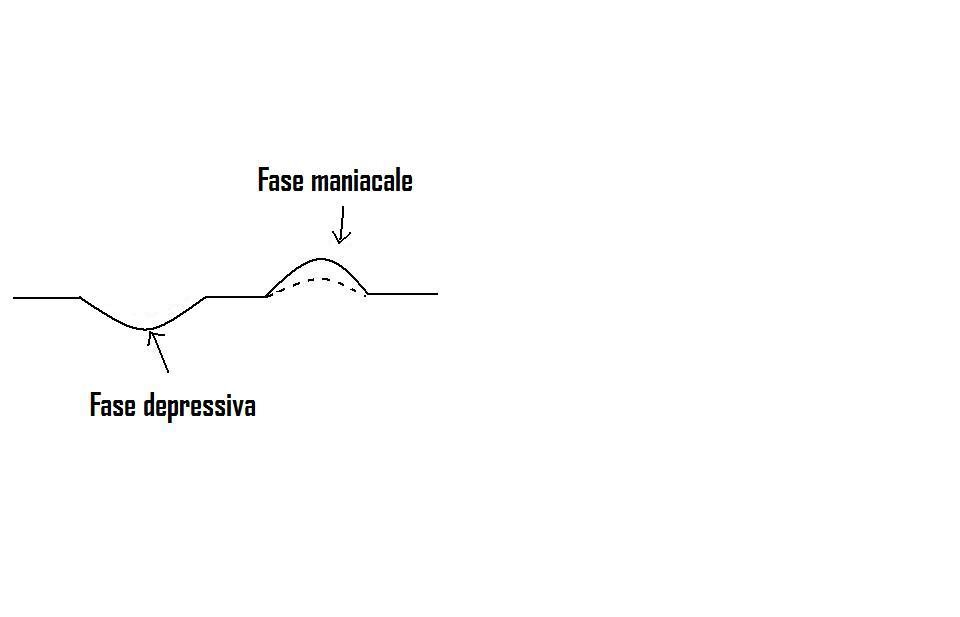
\includegraphics[width=0.9\textwidth]{02/image1.jpeg}
\end{figure}

Posto
che l'umore abbia un tono basale, si possono avere fasi di malattia sul
versante depressivo e fasi di malattia sul versante maniacale oppure
sono fasi depressive o solo fasi maniacali.

\paragraph{DEPRESSIONE MAGGIORE RICORRENTE} vuol dire che quel soggetto ha
solo manifestazioni depressive, è un paziente che non scivola dalla
parte opposta come nel caso del disturbo bipolare. Quindi se io avessi
un episodio depressivo questo potrebbe essere una manifestazione
iniziale di una depressione maggiore ricorrente o la prima
manifestazione di un disturbo bipolare, in questo caso però ho bisogno
di una fase maniacale e fino a quando non ce l'ho non posso fare
diagnosi di disturbo bipolare anche se questa possibilità è presente.
Pensate che si considera che circa il 15-20\% di quei soggetti che fino
a quel momento sono dei depressi maggiori ricorrenti possono diventare
dei pazienti con disturbo bipolare perché si manifesterà un episodio
maniacale.

Questo tipo di disturbo (depressione maggiore ricorrente) viene anche
definito \textbf{DEPRESSIONE UNIPOLARE}, perché le fasi di malattia sono
sempre e solo depressive: l'alterazione dell'umore è solo in questo
senso.

Si devono considerare alcune \textbf{caratteristiche,} per definire il
quadro di DEPRESSIONE MAGGIORE RICORRENTE (in cui la sintomatologia che
abbiamo visto si ripresenta più volte)\textbf{:}

\begin{itemize}
\item[1.]
  \textbf{il numero di episodi} Prendendo una popolazione di soggetti
  depressi il VALORE MEDIANO degli episodi è di 4: il 50\% dei soggetti
  ha da 1 a 4 episodi nella vita e il restante 50\% ha più di 4 episodi
  nella vita. È possibile ci siano pz con fasi numericamente limitate e
  altri con fasi frequenti.
\item[2.]
  \textbf{la durata degli episodi} è variabile. Valutando nella
  popolazione dei depressi la durata, la mediana è di 6 MESI: nel 50\%
  dei pz la depressione dura da almeno (due settimane per definizione) 6
  mesi, nell'altro 50\% dura più di 6 mesi , anche per alcuni anni!
\end{itemize}

\emph{NB: la media è diversa dalla mediana: in quest'ultima si considera
il valore che divide esattamente in due metà numericamente uguali il
campione (quindi non è influenzata dai valori estremi).}

\begin{itemize}
\item[1.]
  bisogna considerare il \textbf{rischio di suicidio} (10\% dei pz tenta
  e riesce) e il rischio aumenta in relazione a: familiarità, delirio,
  maggiore durata episodi e ripetuti fallimenti terapeutici.
\item[2.]
  \textbf{Insorgenza}: depressione ricorrente più facilmente compare
  dopo i 30 anni
\end{itemize}

\paragraph{CRITERI DELLA DEPRESSIONE MAGGIORE:}

Attualmente in Psichiatria vengono usati due sistemi diagnostici :

\begin{itemize}
\item
  \emph{\emph{L'International Classification of Diseases dell'OMS:}} si
  usa abitualmente ed è anche utilizzato per fare diagnosi di
  dimissione.
\item
  L'altro è quello \emph{\emph{dell'American Psychiatric Association}}
  (quinta ed ultima edizione nel 2013): ha avuto un grande e inaspettato
  successo. Quest ultimo è un manuale semplice che presenta vari sintomi
  i quali, se soddisfatti, permettono di arrivare ad un'indicazione
  diagnostica. Tuttavia è molto limitativo in quanto un sintomo ha lo
  stesso valore sia che sia legato alla depressione sia che sia legato
  ad altre patologie perché non indaga sul vissuto del paziente e quindi
  non ci permette di poter differenziare i vari casi.
\end{itemize}

Esempio: ``non uscire di casa'' perchè non si sente il desiderio/
piacere di uscire o perché si teme che fuori capiti qualcosa (stesso
sintomo ma diverse situazione). Come l'animale che ferito torna nella
tana cosi l' inclinazione di tutti quelli che stanno male è di ritararsi
e non stare in mezzo agli altri, non solo perchè sono infastiditi dalla
gente, ma anche perché notano la differenza con gli altri.

Esempio : ``insonnia'' nel paziente depresso si ha insonnia perché
durante la notte si angoscia pensando di essere incapace di svolgere le
funzioni del giorno successivo . Diverso è invece il caso del paziente
che si sveglia perchè ha tanta energia in corpo e quindi freme
nell'attuare i suoi compiti.

Questo è stato un sistema messo a punto, più che per la pratica clinica,
per permettere a chi faceva ricerca di selezionare campioni di pazienti
che avessero lo stesso disturbo, perchè si avevano dei campioni
assolutamente disomogenei. Per cui il tentativo era di scegliere, almeno
per i disturbi sulla depressione maggiore, pazienti che sono simili. Poi
purtroppo se ne è fatto un cattivo uso perché oramai questo viene usato
nella pratica clinica, per la formazione degli studenti, formazione
degli specializzandi. La realtà è diversa e più complessa.

Bisogna quindi analizzare in modo empatico la situazione per comprendere
in maniera corretta il vissuto del paziente e far diagnosi. Questo è il
motivo per cui il manuale , seppur molto in uso , è riduttivo.

Di norma per diagnosticare la Depressione Maggiore: dobbiamo valutare:
1.SINTOMI, 2.DURATA, 3.IMPATTO:

\begin{itemize}
\item
  Devono essere \emph{\emph{presenti contemporaneamente almeno 5 di
  questi nove sintomi:}}
\begin{itemize}
\item[1.]
  \textbf{Umore depresso per la maggior parte del giorno, quasi ogni
  giorno};
\item[2.]
  \textbf{Marcata diminuzione di interesse o piacere per tutte o quasi
  tutte le attività normalmente svolte dal paziente};
\item[3.]
  \textbf{Significativa perdita o aumento di peso o dell'appetito};
\item[4.]
  \textbf{Insonnia o ipersonnia};
\item[5.]
  \textbf{Agitazione o rallentamento psicomotorio};
\item[6.]
  \textbf{Faticabilità o mancanza di energia};
\item[7.]
  \textbf{Sentimenti di autosvalutazione o di colpa inadeguati,
  inappropriati o eccessivi};
\item[8.]
  \textbf{Diminuita capacità di pensare o di concentrarsi o presenza
  di forti indecisioni};
\item[9.]
  \textbf{Pensieri ricorrenti di morte, ricorrente ideazione
  suicidaria o tentativo di suicidio}.
\end{itemize}

Di cui almeno uno deve essere: 
\begin{itemize}
\item[(1)]
l'umore depresso per la maggior parte del giorno o 
\item[(2)]
la perdita di interesse e piacere per quasi tutte le
attività.
\end{itemize}

È ovvio che si deve sempre tener presente che il sintomo non deve essere
spiegato da un'altra patologia (Ad esempio il tumore del pancreas o
l'assunzione di sostanze possono portare ad un'alterazione dell'umore).
Quindi, in altri termini, dobbiamo verificare se è un disturbo
\emph{``primario''} cioè non riconducibile ad altre patologie o
\emph{``secondario''} se invece è dovuto a particolari malattie.

\item
  Deve avere una \emph{\emph{durata di almeno due settimane}} (si parla
  disturbo cronico se superiore a due anni): 2 settimane era un criterio
  necessario per definire il tempo però, gli episodi depressivi sono ben
  lontani da questa durata. Si giustifica questa affermazione partendo
  da questo dato: ammettendo di essere tutti pazienti depressi, di avere
  avuto tutti un episodio depressivo che ha avuto una durata: quindi ha
  avuto un'insolvenza, ha avuto una risoluzione e ciascuno dei pazienti
  ha la sua durata di malattia. Si può fare la media ma più che la
  media, che è esattamente la somma diviso il numero complessivo dei
  pazienti, ci interessa la cosiddetta mediana perchè se si avesse tra
  di loro persone con durate di malattia lunghissima (6 anni) la media
  risentirebbe profondamente di quei 2/3 casi che hanno durate estreme.
  Allora per evitare questo si usa la mediana. Mediana vuol dire quel
  valore che divide il nostro campione in 2 parti numericamente uguali.
  Quindi se si calcola la mediana della durata dell'episodio depressivo,
  si hanno 6 mesi (non 2 settimane). Cosa vuol dire avere una mediana di
  6 mesi come durata di episodio depressivo? vuol dire che se i pazienti
  sono 100, il 50\% del campione ha una durata inferiore ai sei mesi (da
  2 a 6 mesi) ma l'altro 50\% ha una durata di episodi che va oltre i 6
  mesi: infatti tra i disturbi cosiddetti cronici vi è anche la
  depressione maggiore. Tra questi i pazienti che ne sono affetti hanno
  episodi che durano anche altre 2 anni. Quindi se qui 2 settimane è un
  criterio temporale minimo, la realtà o quello che avviene nella
  pratica è ben superiore a queste 2 settimane, quindi almeno circa 24
  settimane. Tenete quindi presente che parliamo di una condizione che
  ha una durata prolungata.
\item
  Deve determinare un \emph{\emph{cambiamento della qualità di vita del
  paziente.}}
\end{itemize}

In realtà la diagnosi non è è sempre così schematica, infatti si possono
avere anche dei quadri di 3 sintomi ma con una depressione gravissima o
quadri con 6 sintomi ma una depressione lieve.

Constatazione: spesso i pazienti depressi non si recano dallo
psichiatra, infatti se prendiamo come esempio un paziente con i sintomi
3 (perdita di peso) , 4 (insonnia) ,6 (faticabilità) il primo sospetto
ricadrà su una patologia tumorale ma, se dopo i dovuti esami, continuano
a mancare le cause organiche sarà necessario riprendere in
considerazione la diagnosi di depressione. Per identificare (screening)
un paziente depresso è sufficiente verificare la presenza di una delle
due prime manifestazioni (sintomo 1 o 2).

Infatti, ricordiamo che dei famosi cinque sintomi almeno uno deve essere
o il primo o il secondo.

Analizziamo i sintomi uno alla volta:
\begin{itemize}
\item[1)]
\emph{Umore triste}: abbiamo una flessibilità stabile dell'umore, ed
il paziente si sente inspiegabilmente triste, cupo, avvilito,
sfiduciato, arrivando nelle forme più avanzate ad essere pessimista,
svuotato, angosciato o anche disperato.
\item[2)]
\emph{Perdita di interesse} : il soggetto diviene insensibile agli
eventi esterni, non è più in grado di provare emozioni e di avvertire le
esperienze piacevoli, condizione nota come \textbf{anedonia.} Un esempio
è il paziente anziano che non esce più di casa e smette di andare al
circolo perchè ha perso la voglia / il piacere / l'interesse / il
divertimento nel farlo. Quello che prima lo spingeva ad andare era il
provare piacere in quell'attività, ora invece avendo perso l'interesse
preferisce restare a casa.

Se analizzati questi due punti permettono di evitare tanti accertamenti
e collegano la sintomatologia ad un quadro di tipo depressivo. La
probabilità che un quadro depressivo venga riconosciuto se il paziente
riferisce astenia , perdita di attenzione , perdita di peso e insonnia è
bassa; diventa alta invece se il paziente piange e ammette la
depressione. Uno studio di dieci anni fa, svoltosi negli Stati Uniti, su
un campione di 300 casi di pazienti affetti depressione maggiore,
dimostra che dal GP ne venivano diagnosticati correttamente solo l' 8\%.
Il trattamento una volta instaurato porta agli stessi esiti sia che il
paziente sia trattato dal medico di medicina generale o dallo
psichiatra. Il problema però è che il medico di medicina generale tende
a sottovalutare la probabilità che quel quadro sintomatologico sia
nell'ambito di un disturbo depressivo.

Importante ricordare che si può anche avere un quadro di depressione in
cui manca la tristezza; infatti è necessario solo uno dei due sintomi
quindi possiamo avere quadri di \emph{\textbf{depressione sine
depressione}:} l'elemento più evidente non è la tristezza ma la restante
sintomatologia.
\begin{itemize}
\item[3a)]
\emph{Inappetenza}: Il calo ponderale è un sintomo importantissmo. Il
paziente affermerà: `` il cibo non ha sapore'', ``mangio perchè so che
devo mangiare ma se seguissi la mia inclinazione non mangerei'', `` il
sapore è amaro''. Questo sintomo è collegato a una perdità del piacere
per cui il cibo non è più una fonte di gratificazione.
\item[3b)]
\emph{Aumento di peso:} in genere in 2/3 dei casi si manifesta
inappetenza , ma in 1/3 dei casi, paradossalmente, si ha un aumento di
peso legato alla tendenza a mangiare di più.
\end{itemize}

\begin{itemize}
\item[4a)]
\emph{Insonnia}: rappresenta uno dei sintomi più precoci e si
manifesta con ripetuti risvegli notturni (\emph{insonnia intermedia}) o,
nelle forme più gravi, con un risveglio precoce, alcune ore prima
dell'orario abituale (\emph{insonnia terminale}). Il sonno, in ogni
caso, non risulta ristoratore, poiché gravato da continui \emph{incubi}
e \emph{sensi di apprensione}. Sono soggetti che vanno a dormire,
riescono ad addormentarsi ma solo dopo poche ore si svegliano angosciati
all'idea delle azioni che dovranno svolgere quella giornata, si sentono
incapaci di svolgere la loro normale routine (che hanno sempre condotto)
e anche le azioni più semplici risultano difficili (un elettricista in
difficoltà a cambiare una lampadina, una casalinga incapace di mettere
la pentola a bollire sul gas) . Il paziente diventa disordinato, non
riesce a fare da mangiare, non riesce a fare nulla e prova un'angoscia
assoluta e senso di colpa che sembrano diminuire verso sera
semplicemente per il fatto che la giornata si è conclusa e non rimane
più nulla da fare.

\item[4b)]
\emph{Ipersonnia}:di solito gli stessi soggetti che mangiano di più
sono anche gli stessi che dormono per più tempo. Non è matematica come
cosa ma spesso è cosi.

Inoltre l'aumento di peso e ipersonnia sembrano collegati a delle forme
\emph{stagionali} cioè depressioni che in genere esordiscono verso
ottobre, quindi nei mesi autunnali, e si risolvono nei mesi primaverili
(simil letargo).
\end{itemize}

\item[5)]
\emph{Agitazione e rallentamento psicomotorio:}Durante un colloquio
vi possono essere pazienti che non riescono a stare seduti quindi si
alzano continuamente o camminano spesso oppure pazienti completamente
immobili, inespressivi e simili a delle statue.

Una caratteristica della depressione maggiore, o disturbo unipolare, è
la CATATONIA:le manifestazioni sono di una gravissima inibizione
psicomotoria, tanto che nelle forme più avanzate si può arrivare a delle
vere e proprie condizioni di arresto psicomotorio, il cosiddetto
``\textbf{stupor melancolicus}'', in cui il paziente rimane immobile a
letto, senza reagire agli stimoli esterni e senza nutrirsi, spesso
avendo anche un blocco della funzione vescicale ed intestinale. Se
proviamo a sollevargli un braccio sentiamo una resistenza che in modo
costante cede alla forza che io applico, a un certo punto se smettiamo
di applicare forza il braccio del paziente rimane sollevato come lo
abbiamo lasciato tant'è che veniva definito ``la flessibilità della
cera''.

E' più frequente trovare catatonie da disturbi dell'umore, soprattutto
bipolare, rispetto a disturbi schizofrenici catatonici.

\item[6)]
\emph{Astenia:} si stancano a svolgere anche le azioni più semplici,
non riescono a condurre la loro normale routine.

\item[7)]
\emph{Sentimenti di colpa e svalutanti}: si sentono incapaci di
svolgere le azioni più semplici e per questo provano un forte senso di
colpa.

È noto che a volte i pazienti depressi sono talmente inibiti che non
riescono neanche a suicidarsi.Questo è vero, succede che il paziente è
talmente inibito che addirittura non riesce neanche a piangere. Questo
si riferisce soprattutto al discorso dell'inibizione, più che altro
motoria,per cui io non riesco neanche a lanciarmi dalla finestra e
neanche ad alzarmi per fare questo.

\item[8)]
\emph{Ridotta capacità di concentrazione o di pensiero}: Le funzioni
cognitive sono alterate, con un marcato rallentamento dell'attività del
pensiero ed una condizione di ottundimento e di mancanza di chiarezza,
spesso associata ad una sensazione di ``avere la testa vuota''; i
contenuti del pensiero, pochi, sono dolorosamente cristallizzati su
pochi argomenti a contenuto melanconico, su cui il paziente ritorna
costantemente (\textbf{ruminazioni mentali} o \textbf{idee coatte}), ed
anche la memoria è intaccata, sia negli aspetti di rievocazione che di
fissazione, tanto che in alcuni pazienti si possono raggiungere delle
condizioni simili a quella della demenza senile. Infatti in passato si
associavano alcuni stati del paziente depresso alla demenza ma con una
possibile regressione. Dal momento che la regressione nella demenza vera
e propria è impossibile è stato coniato il termine di
\textbf{\emph{pseudo demenza}.}

Nel quadro di tipo depressivo il paziente afferma: `` io provo a leggere
ma non c'è verso che mi entri in testa qualcosa''. Tutti questi pazienti
riferiscono infatti oltre alla mancanza di piacere nel fare le cose
anche la mancanza di concentrazione e di attenzione.

I pazienti dementi diversamente con tono non angosciato minimizzano la
situazione cercando di colmare la loro incapacità legata a funzioni
cognitive compromesse. Nei depressi durante i test cognitivi
all'aumentare del tempo o della difficoltà si nota una diminuzione del
risultato dato che non riescono a mantenere la concentrazione. I
pazienti dementi invece cercano in tutti i modi di farcela ( Esempio: il
soggetto demente chiede la data prima del giro visite per non mostrarsi
impreparato quando gli sarà chiesta dal medico). Infine il paziente
depresso non sbaglia mai, il demente invece spesso sbaglia stanza e
compie azioni sconnesse.

\item[9)]
\emph{Pensiero ricorrente di morte, di suicidio}:

\textbf{\emph{Depressione vitale}} : particolare umore che il soggetto
coglie come uno stato d'animo che non ha mai avuto, che lo pervade e che
lo distacca completamente dalla realtà. Non c'è nulla che lo possa
modificare. Si trova in genere associato al \emph{sentimento della
mancanza di sentimento:} '', un angoscioso senso di non provare più
alcunché per le persone o le cose prime care (``\emph{io non provo più
nulla'')}. Un esempio può essere una neomamma che, pur riconoscendo di
avere desiderato con tutta se stessa la figlia, afferma di non provare
nessun sentimento nei sui confronti, a fatica sa che è sua figlia e non
riesce neanche a tenerla in braccio. Questa mancanza di sentimento viene
percepita con un angoscia estrema perché si ritengono cattive madri.

Fondamentale è poi la comprensione di come questi pazienti vivano il
\emph{tempo interiore}, poiché nell'episodio depressivo vi è uno
\textbf{scollamento del tempo cronologico dal tempo interno}: per il
paziente depresso le giornate appaiono interminabili, le ore non
scorrono mai, ed i giorni, i mesi e gli anni a venire sono tutti visti
in chiave negativa, come un tempo di sofferenza infinita da cui spesso
traggono origine le \emph{idee suicidarie}. Quindi \emph{il tempo} in
questi pazienti viene vissuto in un modo particolare: si capisce che il
soggetto si trova in questa condizione di malessere \emph{presente} e
che spesso ripercorre il \emph{passato} vivendolo però con il malessere
emotivo del momento. In altri termini: è come se il passato incombesse
sul presente e nello stesso tempo è come se il presente si fosse
dilatato inglobando nel vissuto anche il passato. Il problema però non è
tanto il passato ma ciò che preoccupa maggiormente il paziente è il
\emph{futuro}.

Per meglio capire il concetto riporto questo esempio: un soggetto di 32
anni ha più o meno una aspettativa di vita di 82-83 anni, quindi sa
potrà vivere per altri 50 anni ma il problema è: come li vivrò? Non vede
soluzione per il suo malessere presente, non vede via di uscita dalla
sua condizione, il presente ingloba anche il futuro. Questa situazione
crea un'angoscia tale per cui, piuttosto che vivere altri 50 anni in
questa sofferenza atroce, preferiscono ``anticipare la data'' vedendo
nel suicidio l'unica via per porre fine al loro dolore.
\end{itemize}

\begin{itemize}
\item
\emph{Esempio1} : Alcuni anni fa in Valle d'Aosta dei turisti, facendo
una passeggiata in un sentiero che fiancheggiava un laghetto, si
accorsero che nel laghetto c'era una donna con due bambini. La madre
raggiunta dai soccoritori disse ``lasciatemi stare , lasciatemi morire
``. Non vedeva soluzione alla sua sofferenza se non la morte. Bisogna
però capire perché ha conivolto nel suo suicidio anche i figli: la madre
era convita che la sua sorte sarebbe toccata anche ai suoi figli per cui
portandoli con sè avrebbe risparmiato loro una vita di sofferenze. (Il
\emph{canto notturno di un Pastore errante dell' Asia} di Leopardi
finisce con : `'è funesto a chi nasce il dì natale'' questa frase per il
depresso è \emph{letterale}.)

Spesso in questi casi si parla di \textbf{\emph{suicidio altruistico}}
perché il paziente è convinto di risparmiare alle persone a cui vuole
bene una vita di sofferenza estrema .

\item \emph{Esempio 2}: 7-8 anni fa a Reggio Emilia un padre uccise il figlio
di 3 anni, la moglie, la vicina di casa che li ospitava gratuitamente e
poi tentò il suicidio ma non riuscì nell'intento di togliersi la vita.
Alla domanda dello psichiatra riguardo il perchè di queste azioni,
affermò: ``l'ho fatto per il troppo amore''. Nell'ottica del paziente
depresso ha risparmiato loro degli anni di sofferenza \emph{suicidio
allargato di tipo depressivo} (Da non confondere con il marito che
uccide la moglie per gelosia che affermerebbe ``Lei o sta con me o non
sta con nessuno'' e non `` l'ho fatto per risparmiarle anni ed anni di
sofferenza'').

\item \emph{Esempio 3}: alcuni pazienti affermano : ``la ringrazio dottore per
quello che fa, ma per me non c'è nulla da fare. Mi salva e io starò
altri 50 anni cosi ? ..mi lasci morire perchè per me non c'è nulla da
fare''.

\item \emph{Esempio 4}: Conclusione: Data tale definizione si dimostra come
nessun paziente con depressione possa comportarsi allo stesso modo del
pilota dell'Airbus Germanwings. Il pilota infatti:

\begin{itemize}
\item
  ha pianificato tutte le sue mosse, un paziente depresso non è capace
  di pianificare ma anzi si sente spesso un incapace.
\item
  Il depresso non è un omidicia, ma un suicida. Può coinvolgere altri ma
  saranno persone da lui molto amate a cui vuole risparmiare il dolore
  che lui sta provando (suicidio altruistico).
\end{itemize}
\end{itemize}

L'episodio depressivo può inoltre caratterizzarsi per la presenza di
\textbf{MANIFESTAZIONI DELIRANTI} (Delirio: dal latino, esco dal solco.
Il solco è il giudizio che ciascuno di noi ha della realtà e è ciò che
appare immediatamente e fa parte del senso comune. L'alterazione nasce e
si genera dall'alterazione dell'umore) , e in questo caso si parla di
\emph{deliri affettivi} o \emph{olotimici}, che possono essere
essenzialmente di 3 tipi:

\begin{itemize}
\item[1.]
  DELIRIO di ROVINA (ECONOMICA): (il paziente crede che, a causa della
  sua condizione attuale, non sarà più in grado di sostenere
  economicamente la sua famiglia, per cui crede di essere sul lastrico
  anche se in realtà è ricco).
\item[2.]
  DELIRIO di COLPA: (il paziente vede la sua condizione di sofferenza
  attuale come la punizione di una colpa compiuta in passato, spesso del
  tutto sproporzionata alla condizione attuale).
\item[3.]
  DELIRIO SOMATICO: (il paziente è convinto di avere una malattia
  incurabile, spesso identificata come causa del suo male, ma crede che
  gli altri vogliano tenerglielo nascosto).
\end{itemize}

Questi tre tipi di deliri possono poi associarsi tra loro costituendo
delle forme particolarmente gravi:

\begin{itemize}
\item
  come il \textbf{\emph{delirio nichilistico}}, in cui il paziente è
  convinto di non avere più una famiglia o addirittura parti del corpo,
  arrivando persino a negare la propria esistenza,
\item
  alla cosiddetta \textbf{\emph{sindrome di Cotard}}, in cui il paziente
  crede di essere morto e dannato a permanere sulla terra per l'eternità
  ad espiare le sue colpe oppure crede di essere l'unico uomo rimasto in
  vita, ma mentre lui soffre sulla terra, tutti gli altri sono in
  paradiso.
\item
  Nelle fasi avanzate non è poi raro riscontrare altre forme di delirio,
  che sono incongrue con l'umore, come il delirio di gelosia (piuttosto
  comune in verità), il delirio di persecuzione, di veneficio, di
  inserzione o furto del pensiero.
\end{itemize}

Queste forme di delirio possono essere OLOTIMICHE (congruenti all'umore)
o NON OLOTIMICHE.

Analizziamo le varie tipologie di delirio riferendoci a particolari casi
clinici:

\begin{itemize}
\item[1.]
  \textbf{\emph{DELIRIO DI ROVINA:}}

Vediamo cosa si intende con esempio:

\emph{Caso clinico}:

Il paziente è un avvocato che è diventato incapace di svolgere il suo
lavoro che ha sempre fatto: afferma di rimanere fermo davanti alle
pratiche e di non riuscire ad andare avanti nella lettura (era un
esordio di depressione). Il problema però non si è limitato a questo:
egli nei giorni seguenti ha cominciato a maturare la convinzione che,
non riuscendo più a fare il suo lavoro, avrebbe perso i clienti e con
questo i soldi e il lavoro con cui manteneva la famiglia. La moglie, di
fronte a questi discorsi fatti dal marito, ha cercato di convincerlo
della mancanza del problema con un dato di fatto: i conti in banca, che
dimostravano che la famiglia non sarebbe comunque andata verso problemi
economici. Tuttavia il pz continua ad insistere. In una delle visite il
pz chiede di parlare senza la moglie presente, dovendo dire una cosa che
sarebbe stata per lei spiacevole: egli era andato in autostrada per
cercare un punto da cui buttarsi. L'avvocato viene trattato (era al 3\textsuperscript{o}
episodio di malattia), guarisce e torna a condurre normalmente la sua
vita fino a quando dopo circa 3 anni una delle sue segretarie lo trova
morto in studio sulla sua scrivania: si era sparato.

\emph{Cos'è successo?} Risolto il precedente episodio di depressione
dopo tre anni aveva avuto una ricaduta. Ripartendo con la stessa
convinzione (ora delirante) di essere la causa della rovina economia sua
e della sua famiglia (si parla di DELIRIO DI ROVINA), si è tolto la
vita.

Consideriamo due aspetti del DELIRIO DI ROVINA:

\begin{itemize}
\item
  Questo delirio viene definito \emph{OLOTIMICO} dalla psichiatria
  classica e delirio CONGRUO ALL'UMORE dalla visione più moderna: se si
  ricostruisce l'esperienza delirante possiamo comprendere questa solo
  sulla base della depressione. Ovvero la depressione aveva causato in
  lui disturbi cognitivi (concentrazione, attenzione), difficoltà a
  raggiungere obiettivi, stanchezza\ldots{} e tutto questo ha generato
  (appunto sulla base della depressione), l'impossibilità di mantenere
  una attività lavorativa e quindi da questo si è sviluppato il delirio
  di rovina. È stato quindi, classicamente, definito ``OLOTIMICO''
  perché è l'alterazione dell'umore che fa da terreno per lo sviluppo
  dell'esperienza delirante stessa delirio \emph{congruo con l'umore}
  appunto perché è insito e nasce dall'esperienza depressiva. Ripetendo
  con altre parole: Il Delirio olotimico è connesso strettamente con
  l'alterazione dell'umore che ci permette di comprendere in termini di
  determinismo come mai il soggetto è arrivato a sconvolgere la realtà.
\item
  Il pz non si suicida al 3\textsuperscript{o} episodio di malattia grazie al trattamento
  ma si suicida al 4\textsuperscript{o} episodio: come è possibile che il pz, pur avendo
  avuto già degli episodi depressivi che si erano risolti, non sia
  riuscito a rendersi conto e a realizzare che si sarebbe ripreso anche
  da questo episodio? Scatta un altro meccanismo: il pz si rende conto
  dell'episodio depressivo (stessi sintomi dei precedenti), ma in questo
  egli non ha più la speranza, si convince del fatto che gli altri
  episodi non fossero come questo (in realtà l'episiodio è uguale ai
  precedenti) e che non ci sia più futuro o possibilità di cambiare la
  situazione attuale. Questo fa sì che le idee suicide, presenti anche
  negli episodi precedenti, siano portate a compimento. Dal punto di
  vista del pz l'episodio è diverso e non è possibile uscirne, non c'è
  futuro.
\end{itemize}

\item
  \textbf{\emph{IL DELIRIO DI COLPA:}}

Le ragioni della colpevolezza possono essere le più svariate, sia per
gesti fatti che per quelli non fatti.

\emph{Caso clinico 1:}

Il paziente è una donna che ha appena partorito. Guardando la storia
clinica della paziente apprendiamo che intorno al 7\textsuperscript{o} mese la pz si era
presentata al PS chiedendo di partorire nella totale convinzione che il
figlio stesse male. Viene fatta una visita ginecologica, tutto risulta
nella norma, la pz viene rassicurata e mandata a casa. Il giorno dopo di
nuovo si presenta e di nuovo vengono fatti accertamenti: non c'è niente
di irregolare, quindi il ginecologo decide di chiamare uno psichiatra
per la pz, ma questa non accetta e va a casa. Non si sa più nulla fino a
dopo il momento del parto in cui alla visita pischiatrica afferma:
\emph{``avete già dato in adozione mio figlio?''.} Viene indicato il
ricovero, la pz accetta.

Perché la pz ha detto questa frase?

Il problema è che la pz non si sente adeguata, è convinta di non potere
essere una buona madre. Vediamo l'estrema conseguenza di questi pensieri
e di questo stato d'animo, infatti la pz vive la gestazione pensando di
essere tanto incapace che anche il suo corpo non sia adeguato allo
sviluppo del bambino: il suo utero era inadeguato per il figlio, non era
lui malato ma lei che lo poteva far ammalare.

\emph{Caso clinico 2}: una pz che in episodio depressivo si è
colpevolizzata per aver preso alcuni sassi da un torrente durante una
passeggiata.

\item[3.]
  \textbf{\emph{IL DELIRIO DI PERSECUZIONE:}}

\emph{Non è olotimico}, a meno che non ci sia effettivamente la
possibilità di identificare una causa alla base (effettivamente il pz ha
commesso un atto che ``giustifica'' questi pensieri, che ci permette di
distinguere il deliro di colpa dal delirio di persecuzione propriamente
detto).

\emph{Caso clinico:}

Ragazzo di 23 anni ricoverato per episodio depressivo. Egli era orfano e
viveva con il fratello. Qualche mese prima dell'esordio depressivo erano
accaduti una serire di eventi: il fratello, avendolo visto fumare
marjuana lo aveva ammonito a smettere o avrebbe allontanato da casa; la
fidanzata, sempre per la stessa ragione, aveva minacciato di lasciarlo;
il datore di lavoro, dato il suo comportamento poco responsabile al
lavoro, aveva minacciato il licenziamento. Mentre era ricoverato, una
notte è stato trovato intento a tagliarsi i polsi con la lametta del
rasoio. Quale è stata la ragione di questo suo gesto? Egli ha riferito
di avere sentito le sirene dei carabinieri che lo sarebbero venuto a
prendere (notate che in realtà erano le sirene della ambulanze della
croce rossa, lì a fianco), processare, condannare e imprigionare per
quello che aveva fatto (quindi si sarebbe ammazzato piuttosto).

\textbf{Come facciamo a discriminare se in questo caso si tratta di
delirio di colpa o di delirio di persecuzione?} È stato chiesto al pz se
avesse fatto qualcosa che giustificasse tutto ciò ed egli ha riferito
quello che aveva fatto (e che giustifica il DELIRIO DI COLPA, ``è giusto
che io sia giustiziato per quello che ho fatto''). \emph{Invece nel
delirio di persecuzione i soggetti dicono di non sapere perché la
Giustizia se la prenda con loro}.

\item[4.]
  \textbf{\emph{IL DELIRIO SOMATICO}}:

Il delirio somatico può essere:

\begin{itemize}
\item
  riferito al pz
\item
  riferito ai famigliari (ad es una donna che si era convinta del fatto
  che il figlio avesse la leucemia\ldots{})
\end{itemize}

Quindi a volte il vissuto somatico è talmente alterato dagli episodi
depressivi che ciò che riferiscono i pz ha le caratteritiche del
delirio. Lo si riscontra soprattutto nell'anziano, quando il corpo
invecchia e il soggetto si rende conto di questi problemi.

Per capire di cosa si tratta si vedano questi esempi:

\emph{Caso clinico 1:}

Marito e moglie, circa 60 anni. Il marito esce di casa e quando torna
trova la moglie in piedi davanti al lavello con i polsi tagliati
profondamente (arteria e tendini) \emph{notate che caratteristicamente
in questi casi il pz prepara stracci e sta sul lavello per non
sporcare}. Il marito riferisce di non essersi accorto di nulla, non
trova spiegazione.

Viene poi ricostruita la storia con la pz: aveva avuto una crisi
epilettica qualche mese prima, non si è scoperta la causa (non aveva
tumori, nulla..), ma le si era insinuato il dubbio di avere un tumore e
che gli altri non volessero dirglielo: si convince di avere pochi mesi
di vita e decide di suicidarsi piuttosto che arrivare allo stadio
terminale della malattia.

\emph{Caso clinico 2:}

Pz depressa che è convinta di avere una fistola tra l'esofago e la
trachea perché avverte un odore di putrefazione, causato dal cibo che
passa in trachea a causa della fistola e si deposita nelle basi
polmonari dove va in putrefazione.

\emph{Domanda studente: l'ipocondria fa parte del delirio somatico?}

Generalmente il vissuto somatico del depresso è tutto alterato: è un pz
che dimagrisce, è deperito, etc, quindi il medico potrebbe pensare che
abbia di tumore e anche il pz si convince di ciò\ldots{}poi si arriva
fino al vero e proprio delirio.
\end{itemize}

\paragraph{EZIOPATOGENESI DELLA DEPRESSIONE MAGGIORE:}

\begin{figure}[!ht]
\centering
	\includegraphics[width=0.9\textwidth]{02/image2.jpeg}
\end{figure}

Come non esiste un esame che ci permetta di fare diagnosi così non ho
nemmeno un'idea precisa sulle cause, ma sappiamo che esistono per
ciascun disturbo dei fattori di rischio.

La stragrande maggioranza dei disturbi psichiatrici non hanno
un'eziologia unica: \textbf{ci muoviamo nell'ambito dell'eziologia
multifattoriale}.

Cosa intendiamo per rischio? Utilizziamo una metafora.

Nel momento in cui noi siamo stati concepiti ci è stato consegnato un
recipiente, un'anfora che può avere o non avere una determinata quantità
di liquido dentro; il liquido rappresenta i fattori di rischio. Tanti
più fattori di rischio ho, tanto è più probabile che il livello del
liquido si avvicini al colmo dell'anfora e travasi. Fintantoché ho solo
liquido e non tracima, io rimango nell'ambito della vulnerabilità, del
rischio, ma non ho la malattia; quando tracima passo dal rischio alla
malattia.

I fattori di rischio possono non essere presenti sempre in un dato
momento ma si possono aggiungere in fasi successive: ne posso avere al
momento della nascita, se ne possono aggiungere nei primi anni di vita,
durante l'adolescenza e anche in età adulta. Più se ne aggiungono più è
probabile che la mia anfora tracimi. Se non tracima non mi ammalo, però
attenzione perché quel rischio io lo trasferisco e lo consegno ai miei
figli, una sorta di eredità.

I rettangoli nella slide sono tutti fattori di rischio conosciuti;
esistono alcuni fattori protettivi: come il supporto sociale che mi
``tolgono liquido''. Questi fattori di rischio sono interconnessi, si
influenzano.

Vari studi hanno ormai messo in luce con chiarezza che si tratta di un
\textbf{\emph{processo eziopatogenetico complesso}}, in cui rientrano
sicuramente delle componenti di \emph{ereditarietà}, che predispongono
allo sviluppo del disturbo dell'umore, ma su cui vanno poi ad agire
anche altri fattori, quali il \emph{sesso}, gli eventuali \emph{eventi
traumatici precoci}, lo \emph{stress}, i \emph{fattori socio-economici e
culturali}, le \emph{malattie somatiche} e la \emph{personalità} del
paziente stesso.

\subparagraph{EREDITARIETA'}

Prendiamo in esame una serie di studi che ci permettono di analizzare il
contributo genetico nei confronti della depressione maggiore (modello
adattabile anche a tutti gli altri disturbi psichiatrici in generale).

\begin{itemize}
\item[1.]
  Intervista strutturata a \textbf{100 persone prese a caso} che
  dovrebbero rappresentare la popolazione generale per verificare quanti
  di questi sono stati affetti da depressione maggiore nell'ultimo anno.
  Il dato va dal 4\% dei maschi al 9\% delle femmine con valori
  intermedi attorno al 6\%
\item[2.]
  Cambio popolazione\textbf{: 100 famigliari di primo grado} di un
  paziente affetto da depressione maggiore. La percentuale di quanti ne
  sono affetti è decisamente più alta rispetto alla popolazione
  generale, il che vuol dire che in quella famiglia c'è qualcosa che
  predispone i suoi componenti alla depressione maggiore. Si è dibattuto
  per anni su questo: se fosse più la genetica o l'ambiente ad influire.
\item[3.]
  Studio sulle coppie di \textbf{gemelli}: confronto circa la
  \emph{concordanza} tra gemelli omozigoti ed eterozigoti; cioè ammalato
  uno qual' è la probabilità che sia ammalato anche l'altro. L'idea di
  fondo è che, se si tratta di una malattia con base genetica rilevante,
  mi aspetto che la concordanza tra fratelli omozigoti (DNA identico)
  sia molto più alta rispetto alle coppie di fratelli eterozigoti.
  Questo è stato confermato. Emerge però un dato: la concordanza non è
  del 100\% sappiamo quindi che la genetica ha un ruolo, ma non ci
  spiega perché quel soggetto è malato; inoltre non posso sapere se
  questi due gemelli che vivono con una madre depressa non siano stati
  influenzati maggiormente da questo fattore ambientale?
\item[4.]
  Studio condotto sui \textbf{figli adottivi}. Sono messi a confronto
  due gruppi di bambini adottati da famiglie senza disturbi; la
  differenza tra i due campioni sono i genitori biologici: quelli di un
  gruppo presentano madre o padre o entrambi affetti da depressione,
  quelli dell'altro no. L'unica differenza quindi è la dotazione di
  base, vulnerabilità per la malattia di un gruppo ricevuta dai
  genitori. L' idea è che in questo modo si possa valutare se abbia un
  peso maggiore la vulnerabilità genetica famigliare o l'ambiente. Nel
  primo caso analizzando i bambini da grandi dovrei riscontrare una
  percentuale maggiore di malati di depressione nel gruppo di individui
  vulnerabili; nel secondo caso qualora l'ambiente famigliare riesca ad
  annullare la vulnerabilità avrei un pareggio e, quindi, percentuali
  vicine a quelle della popolazione generale. Vince la vulnerabilità.
\end{itemize}

\begin{figure}[!ht]
\centering
	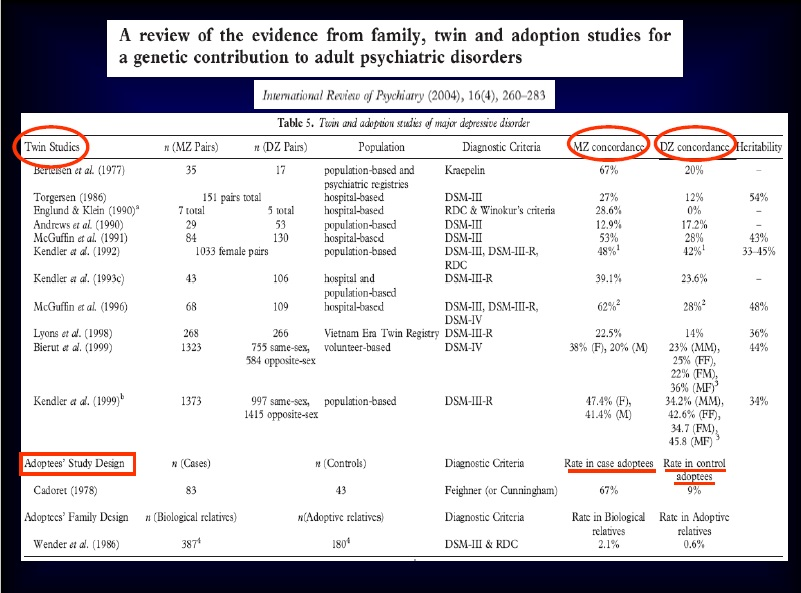
\includegraphics[width=0.9\textwidth]{02/image3.jpeg}
\end{figure}

Quello che emerge è che l'ereditarietà è uno dei fattori che dobbiamo
considerare attentamente. Non è detto, tornando alla metafora, che la
quantità di liquido sia uguale per tutti in termini di rischio genetico:
pensiamo ad esempio ad un figlio concepito da una coppia in cui uno dei
due genitori sia \textbf{bipolare}, la sua anfora è già piena per il
70\%; cosa analoga per la \textbf{schizofrenia}. L'influenza è molto
meno marcata per la \textbf{depressione maggiore} e i \textbf{disturbi
d'ansia}.

In realtà la situazione è più complessa: all'interno della schizofrenia
ad esempio non è detto che tutti ricadano nella stessa percentuale di
rischio genetico. Ciò si può osservare direttamente sui pazienti: padre
schizofrenico con 4 figli, tutti e 4 malati di schizofrenia, padre
schizofrenico con due figli gemelli eterozigoti che si sono ammalati a
distanza di 15 giorni uno dall'altro ed è chiaro che in questi due casi
il peso della genetica sia determinante; in altri casi invece no, ad
esempio tre figli di cui uno solo si ammala (vedi figlio di Gianni
Agnelli che si è buttato da un ponte). La penetranza di questo che non
sappiamo tutt'oggi che gene sia, su quale cromosoma, è variabile tanto
da determinare in alcuni casi un impatto devastante in altri molto meno.
Questo è un problema che viene sollevato dagli stessi pazienti nel caso
in cui, ad esempio vogliano un figlio e vi chiedano ``diventerà
esattamente come me?''. Quella che dobbiamo fornire è un'informazione
corretta riguardo l'accertato fattore di rischio, sulla base della quale
possano decidere liberamente.

\subparagraph{SESSO}

\begin{figure}[!ht]
\centering
	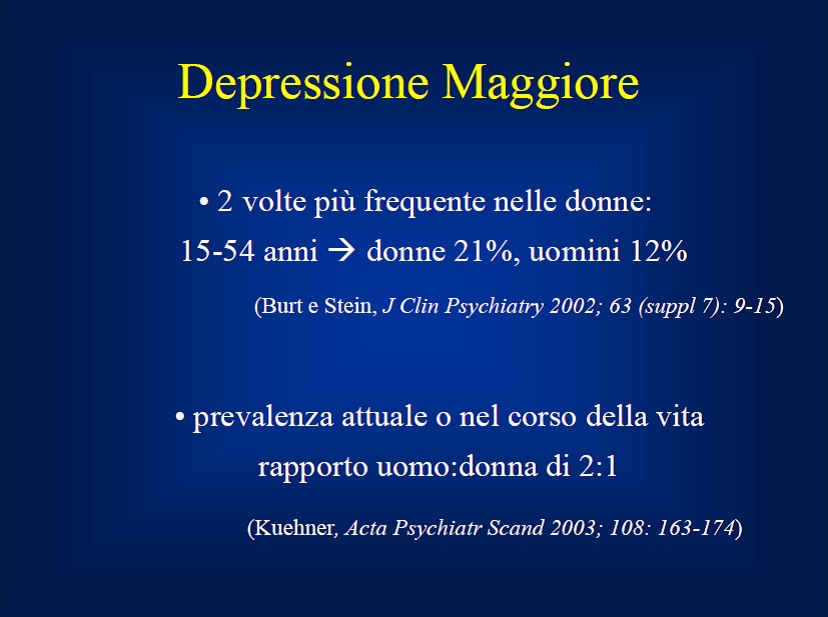
\includegraphics[width=0.9\textwidth]{02/image4.jpeg}
\end{figure}

Tra i 15 e i 54 anni il 21\% (quindi 1 donna su 5) soffrirà di un
episodio depressivo maggiore, contro il 12\% (quindi la metà, 1 su 10
degli uomini). Questo vale per tutta la vita.

Si sono effettuati degli studi sui bambini con grande difficoltà, dovuta
al fatto di studiare la depressione su un bambino che non dice mai
``sono triste'' e quindi bisogna prestare attenzione al suo
comportamento: contatto con gli altri, loquacità, ecc. La cosa
interessante emersa è che l'incidenza tra i bambini tende ad essere
simile indipendentemente dal sesso. Questo fino ai 14 anni circa, ovvero
l'età del menarca in cui questa differenza compare e si mantiene: in
qualche modo \textbf{gli ormoni sessuali sono implicati}.

Studio in cui si è andato a valutare l'effetto di un trauma micidiale
come la violenza sessuale nei bambini e qual era l'effetto di questo
trauma per la vita adulta

\begin{figure}[!ht]
\centering
	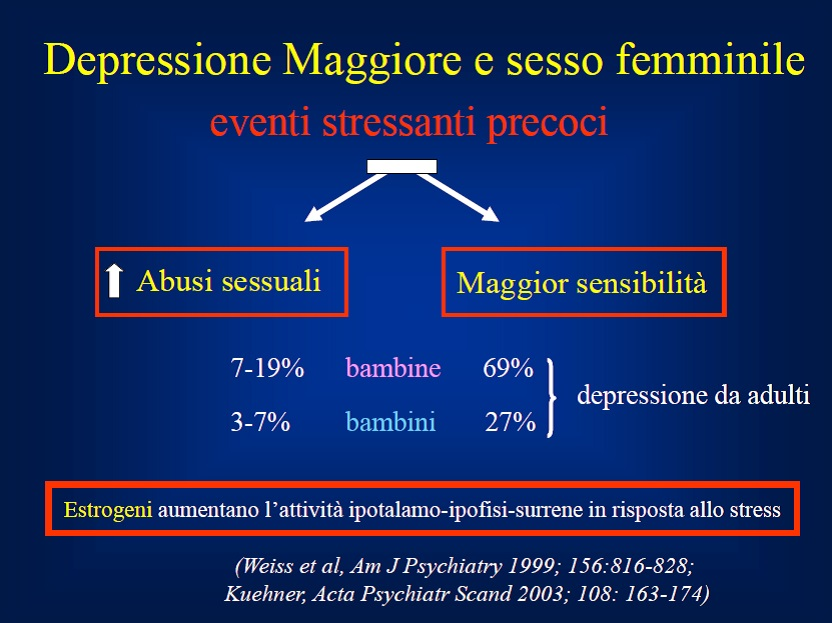
\includegraphics[width=0.9\textwidth]{02/image5.jpeg}
\end{figure}

Risulta rilevante come i 2/3 delle femmine abusate abbia sviluppato un
episodio depressivo contro 1/3 dei maschi, quindi a parità di gravità
dell'evento traumatico le femmine sembrano essere meno resistenti. La
spiegazione chiama in causa il nostro sistema di risposta ad un insulto
esterno, stress: \textbf{l'asse ipotalamo ipofisi surrene} che va visto
come un sistema che permette di affrontare i cambiamenti. Il problema è
che questo sistema viene sensibilizzato dalla presenza degli estrogeni,
il che vuol dire che, a parità di stimolo, l'attivazione è molto
maggiore se ci sono estrogeni e analogamente a parità di risposta basta
uno stimolo minore. Il ``burattinaio'' implicato sarebbe il CRF
(corticotropin-releasing factor) e ciò è interessante per due motivi.

\begin{itemize}
\item[1.]
  Iniettando questa proteina nella scimmia osservo una cosa molto
  interessante, ovvero che l'animale non sta più con gli altri, non si
  alimenta più come prima, non esplora più il territorio, non si
  accudisce come prima e se ha dei piccoli li trascura, il che pur
  parlando di una scimmia ci ricorda aspetti del malato di depressione
  maggiore. Sono stati studiati dei farmaci antidepressivi capaci di
  bloccare l'effetto del CRF, supportati anche dal fatto che nelle forme
  più gravi di depressione si sono dosati dei livelli di cortisolo
  abnormemente elevati , con perdita ritmo circadiano giorno-notte.
\item[2.]
  Questo sistema è quello che ci fa ricordare i traumi e tra gli eventi
  che possono far tracimare l'anfora contenente i fattori di rischio ci
  sono proprio questi scossoni, eventi traumatici. Sistema che si attiva
  immediatamente ed è il momento in cui è molto più facile che l'anfora
  si rovesci, rendendosi manifesta la malattia. Molto probabilmente
  questo sistema si è sviluppato in tal modo a fini evolutivi: è la
  femmina ad avere le prole e necessita di reazioni molto più rapide
  agli stimoli esterni per proteggere la prole.
  \end{itemize}
  
\subparagraph{EVENTI TRAUMATICI PRECOCI}

\begin{figure}[!ht]
\centering
	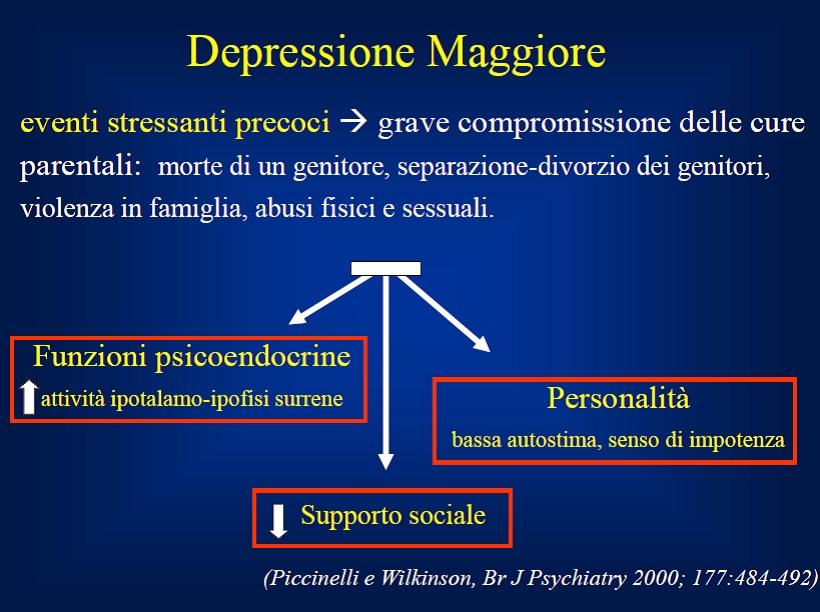
\includegraphics[width=0.9\textwidth]{02/image6.jpeg}
\end{figure}

\textbf{Consistono in tutto ciò che mette gravemente in crisi le cure
parentali}

\begin{itemize}
\item
  Malattie di un genitore
\item
  Morte di un genitore
\item
  Violenze in famiglia
\item
  Abusi fisici e sessuali
\end{itemize}

Non ci riferiamo ad eventi minori come il sospetto che mia mamma non mi
abbia voluto bene, abbia preferito mia sorella mio fratello o mi volesse
bionda; non è questo.

\emph{Considerazione sulle adozioni: è frequente riscontrare numerosi
eventi traumatici nella vita dei primi anni dei ragazzi adottivi; quello
che hanno vissuto potrebbe agire su un terreno geneticamente predisposto
ed ecco che i fattori di rischio che portano alla manifestazione della
malattia si accumulano. Per questo sarebbe opportuno fornire precise
informazioni circa i fattori di rischio alle famiglie che intendono
intraprendere un percorso di adozione, in maniera da poter effettuare
una scelta in maniera consapevole}. \emph{Il nostro cervello assorbe
anche quello che viene dall'ambiente. L'adozione non è una passeggiata,
l'ambiente famigliare non riesce ad annullare tutto ciò che hanno
vissuto nei primi mesi di vita e com'è il loro funzionamento cerebrale,
anche in relazione alla loro vulnerabilità ereditata dai genitori.}

\subparagraph{PERSONALITA'}

Per la depressione vale molto come fattore di rischio l'incapacità di
gestire le situazioni sociali.

Si può spiegare con una metafora: il mio modo di essere con gli altri è
come se fosse un auto, con un acceleratore che la fa muovere ed un freno
che ne riduce la velocità impedendole di andare a sbattere; se io ho un
sistema frenante molto più sviluppato del sistema di accelerazione
faccio molta fatica a muovermi. Il sistema frenate rappresenta il
timore, per esempio, di sbagliare, il timore di che cosa diranno gli
altri, il timore di rimetterci, essere danneggiato dalle scelte che
posso fare: allora sono molto cauto, circospetto, vado molto piano.
All'eccesso questo comportamento determina un disastro in termini di
situazioni sociali: è facile che abbia bisogno di qualcuno che faccia
andare l'acceleratore, di dipendere dagli altri. Questo determina una
forte compromissione delle abilità sociali, difficoltà a muoversi con
gli altri, inserito spesso in un quadro di regole assolute, rigide alle
quali il mondo deve aderire, scarsa flessibilità ed adattabilità agli
eventi esterni.

\begin{figure}[!ht]
\centering
	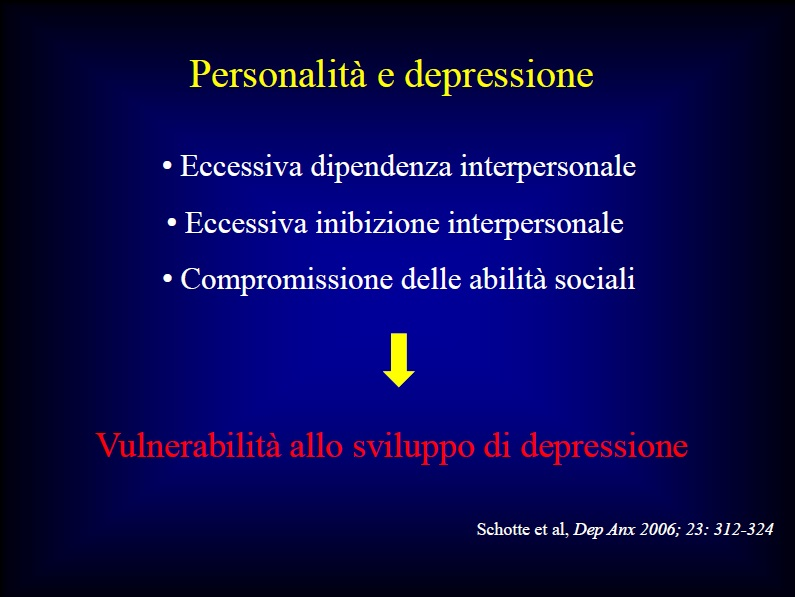
\includegraphics[width=0.9\textwidth]{02/image7.jpeg}
\end{figure}


\subparagraph{DISTURBI DI ANSIA}
Esiste una relazione tra disturbi depressivi e ansiosi

\begin{figure}[!ht]
\centering
	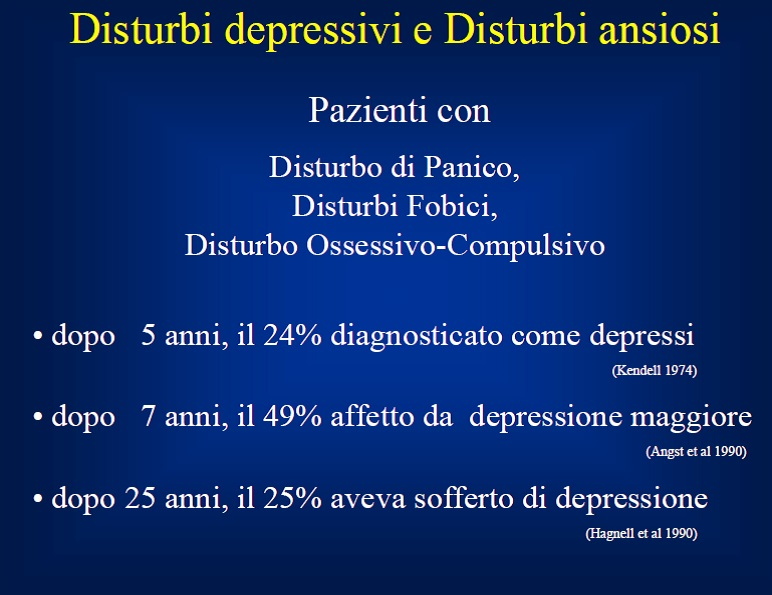
\includegraphics[width=0.9\textwidth]{02/image8.jpeg}
\end{figure}

I disturbi d'ansia possono rimanere tali ma più spesso cambiano, dopo 5
anni un quarto viene diagnosticato come depresso, dopo 7 anni
addirittura la metà. Il che vuol dire che, se io ho un disturbo d'ansia,
è facile che dopo alcuni anni sviluppi un episodio depressivo, anche
perché nella stessa famiglia disturbi ansiosi e depressivi vanno un po'
a braccetto: la famigliarità per uno mi espone ad un rischio anche nei
confronti dell'altro.

Se tolgo l'effetto dell'ansia, la differenza tra sesso maschile e
femminile si riduce del 50\% sulla frequenza di depressione: significa
che il fatto di aver sofferto d'ansia (ancora maggiore incidenza
femminile) è un fattore importante per aumentare nelle donne il rischio
di ammalarsi di depressione maggiore.

\subparagraph{DISTURBI SOMATICI}

Qui in realtà, se andiamo ad analizzare il profilo depressivo associato
a malattie somatiche, notiamo quadri abbastanza diversi dalla
depressione vera e propria, melanconica, presa in considerazione finora.

Interessante è quello che succede quando io ho una forma anche molto
lieve di depressione, addirittura sintomi che non arrivano alla soglia
della diagnosi vera e propria: l'impatto sull'evoluzione della malattia
è nefasto. Consideriamo uno studio su pazienti che hanno malattia
coronarica: tra questi quelli che hanno manifestato anche solo
\textbf{sintomi} depressivi in seguito alla manifestazione coronarica
sono soggetti ad una mortalità praticamente doppia rispetto agli altri.
Monitorando 100 pazienti in unità coronarica che hanno avuto un infarto,
alcuni di questi entro pochi mesi in genere manifestano sintomi
depressivi. A distanza di un anno si evidenzia che questi ultimi hanno
una probabilità doppia di essere deceduti rispetto agli altri; se alcuni
hanno manifestato una maggiore intensità di depressione (soglia
diagnostica) della durata di 3-6 mesi vado leggermente sopra al doppio,
da 6 mesi mi avvicino al triplo come probabilità di decesso. Peggioro
decisamente il decorso ed esito del disturbo coronarico, come anche di
tutte le patologie cerebrovascolari. Si sono evidenziati alcuni
meccanismi eziopatogenetici: non è tanto o solo perché il paziente non
prenda la terapia e non mantenga gli stili di vita corretti; la
depressione modifica l'aggregabilità delle piastrine, modifica l'heart
rate variability, l'attività elettrica cardiaca, l'attività delle
interleuchine e la cascata pro infiammatoria, i livelli di cortisolo e
noradrenalina. Quindi interverrebbe pesantemente nella patogenesi dell'
infarto e delle malattie cardiache.

\subparagraph{FATTORI SOCIO-CULTURALI}

\begin{figure}[!ht]
\centering
	
\includegraphics[width=0.9\textwidth]{02/image9.jpeg}
\end{figure}

Secondo alcuni la depressione sarebbe più frequente negli ultimi anni
rispetto a 100-50 anni fa. In parte è vero e l'incremento riguarda in
particolare le forme minori, più lievi. Uno psicologo ha preso in
considerazione l'odierna società, evidenziando come (specie in quella
occidentale) si abbiano è vero più possibilità economiche, ma anche
molta meno sicurezza sociale: lavoro, cambiamenti di ruolo, rete
sociale. Basti pensare a come il modello di famiglia odierno sia
diverso, per esempio, dalla famiglia patriarcale di una volta del mondo
contadino, dove c'erano 17-18 componenti e in cui, se uno non stava
bene, subentravano gli altri. Chiaramente questo modello paga un effetto
collaterale, ovvero il capofamiglia che decide per tutti, però li vi era
un supporto. Oggi la famiglia media italiana si compone di meno di 2
elementi: se uno si ammala ci si ritrova da soli. Se ci si ammala
bisogna riprendersi alla svelta, perché non c'è nessuno che possa
prendere il nostro posto e in queste condizioni diventa difficile
recuperare completamente. Bisogna considerare che anche queste forme
lievi hanno un certo impatto sul mio funzionamento e che non durano
pochissimo: parliamo di 3-4 settimane, a volte anche di più. Si ha la
possibilità di recupero? L'aumento, se è vero, c'è per le forme più
lievi ma le forme più gravi rimangono piuttosto stabili.

\subparagraph{Eventi stressanti}

Stiamo parlando del momento in cui passo dalla vulnerabilità alla
malattia.

Eventi di \textbf{perdita,} che può essere una perdita \emph{reale}:
morte di una persona a me cara o \emph{simbolica}, perdita del lavoro,
mancato raggiungimento di un obiettivo che il soggetto ritiene
importante, \textbf{elevati conflitti}. Sono tutti molto frequenti prima
di un episodio depressivo e rappresentano, molto probabilmente, il
momento in cui l'anfora tende a tracimare.

È sorto il problema di stabilire se l'evento sia \emph{reattivo}; è
possibile che vi siano episodi che intervengono nella vita di un
soggetto come fulmini a ciel sereno, però spesso c'è qualcosa che ci
induce quel meccanismo. Più che parlare di depressione reattiva, una
definizione un po' passata, interessa la sintomatologia perché quanto a
relazione tra evento di vita e quadro depressivo è molto più frequente
che ci sia un evento di vita, ma questo non vuol dire che quel quadro
sia comunque reattivo a quell'evento. In genere in passato \emph{la
depressione reattiva}, che si trova ancora nella classificazione, aveva
un particolare pattern sintomatologico: il soggetto era si triste ed
ansioso ma tutta la sua vita, quindi il suo umore, quello che pensava,
andava comunque a finire su quell'evento. Un esempio: mi lascio con il
fidanzato, quindi non sono allegro, faccio fatica a dormire. Se provo a
vedere tutto quello che penso e che mi impedisce di addormentarmi, noto
che può essere l'idea che forse ho sbagliato, forse sarebbe stato meglio
se avessi fatto questo, e non se avessi fatto quest'altro, ecc (la
cosiddetta \emph{polarizzazione dell'evento}).

Se considero invece un episodio depressivo come quelli presentati nelle
scorse lezioni (come l'avvocato per intenderci), posso aver avuto un
evento come il calo dei clienti, ma dall'esser calati i clienti a dire
che tutto corre solo ed unicamente su quel filone ce ne passa: non è
tutto legato a quell'evento.

È molto più frequente che io abbia un \emph{trigger} che innesca
l'episodio, mentre è molto meno frequente che quel quadro depressivo sia
strettamente connesso come sintomatologia, come manifestazione a
quell'evento: è possibile, ma raro.

Per \textbf{depressione reattiva} intendiamo quando un quadro
sintomatologico ha un'espressione in cui tutto quello che vive il
paziente è strettamente connesso, polarizzato su quell'evento.

Gli eventi di vita che abbiamo preso in considerazione sono invece
inneschi per trigger.

Una considerazione importante è sorta studiando il disturbo bipolare, in
cui si è visto che è molto più facile che gli episodi di malattia
iniziali siano in qualche modo scatenati da degli eventi. Man mano che
io avanzo si perde questa successione tra stimolo ed episodio; viene
meno l'effetto trigger di un evento e quindi è più facile che gli
episodi partano quando hanno voglia loro, in modo quasi spontaneo.

In un esperimento si sono provocate delle crisi epilettiche ad un
animale da esperimento con la stimolazione elettrica: dopo un certo
numero di scosse l'animale fa le crisi epilettiche da solo. Il modello
applicato al disturbo bipolare è che si ha inizialmente uno stimolo e
successivamente l'episodio; dopo un certo numero di stimoli il mio
cervello mette in atto delle crisi indipendentemente dallo stimolo
esterno.

\textbf{Chiaramente i fattori di rischio devono modificare il
funzionamento cerebrale: la risonanza magnetica funzionale di uno stesso
paziente fatta quando lui sta bene (in eutimia) e fatta quando è
depresso, non è la stessa}.

Consideriamo uno studio fatto dal professor Parmigiani con la
collaborazione dell'unità di psichiatria sui topi, i quali hanno un
sistema gerarchico in cui il ``topo secondo'' non attacca il ``primo''.
Ad un certo punto è stato iniettato del viagra al topo secondo, che
attacca e vince il primo. L'ex topo primo si mette in disparte con la
coda tra le gambe. Gli hanno tagliato la testa e sono andati a vedere
cosa succedeva nel cervello: il dosaggio del BDNF (fattore di crescita
neuronale) risulta abbassato, le aree ippocampali si sono ridotte. Il
sistema cerebrale del povero topolino si è modificato e questo soltanto
in forza di uno stimolo sociale, ambientale: ha cambiato solamente di
rango. Il nostro sistema cerebrale non è autonomo, non è sigillato
dall'ambiente, altrimenti non si capirebbero tutti questi fattori di
rischio che modificano il funzionamento del nostro cervello.

Per quanto riguarda i meccanismi che sono alla base dell'insorgenza
della manifestazione depressiva, vari studi hanno ormai messo in luce
con chiarezza che si tratta di un \textbf{\emph{processo
eziopatogenetico complesso}}, in cui rientrano sicuramente delle
componenti di \emph{ereditarietà}, che predispongono allo sviluppo del
disturbo dell'umore, ma su cui vanno poi ad agire anche altri fattori,
quali il \emph{sesso}, gli eventuali \emph{eventi traumatici precoci},
lo \emph{stress}, i \emph{fattori socio-economici e culturali}, le
\emph{malattie somatiche} e la \emph{personalità} del paziente stesso.

\subsubsection{Altre forme di depressione}

Accanto alla Depressione Maggiore, che rappresenta comunque il quadro
clinico più comune e rilevante dal punto di vista epidemiologico, in
base ai criteri del DSM sono state stabilite anche alcune varianti
dell'episodio depressivo, rispettivamente la \emph{depressione con
manifestazioni melanconiche}, la \emph{depressione con manifestazioni
psicotiche}, la \emph{depressione con manifestazioni catatoniche}, la
\emph{depressione con manifestazioni atipiche}, la \emph{depressione
breve ricorrente} e la \emph{depressione minore}.

\paragraph{Depressione con Manifestazioni Melanconiche}
  Corrisponde essenzialmente con la vecchia depressione endogena della
  nosografia classica, e si caratterizza per la \emph{peculiarità e la
  gravità dei sintomi}, nonché per la \emph{buona risposta ai
  trattamenti somatici} (TEC e antidepressivi), per l'\emph{assenza di
  eventi scatenanti} e per il \emph{buon funzionamento della personalità
  in epoca premorbosa e nelle fasi di remissione}.

  Secondo i criteri del DSM-IV, si può parlare di depressione
  melanconica quando vi è almeno uno dei seguenti sintomi principali:

\begin{itemize}
\item
  \emph{Perdita di piacere per tutte o quasi tutte le attività
  quotidiane;}
\item
  \emph{Perdita di reattività agli stimoli abitualmente piacevoli.}
\end{itemize}

In più, devono anche essere presenti almeno \emph{3 dei seguenti
sintomi}:

\begin{itemize}
\item
  \emph{Una specifica qualità dell'umore depresso, che risulta quindi
  nettamente distinto dal tipo di sentimento provato ad esempio dopo la
  perdita di una persona cara;}
\item
  \emph{Depressione regolarmente peggiore al mattino;}
\item
  \emph{Risveglio precoce al mattino} (almeno 2 ore prima del solito);
\item
  \emph{Marcato rallentamento motorio o agitazione;}
\item
  \emph{Anoressia o perdita di peso;}
\item
  \emph{Sentimenti di colpa inappropriati o eccessivi.}
\end{itemize}

\paragraph{Depressione con Manifestazioni Catatoniche}
In questo
  sottotipo sono in primo piano i \emph{sintomi psico-motori}, come il
  grave rallentamento che può arrivare sino alla catalessia, alla
  flessibilità cerea ed allo stupor. Non sono rari nemmeno i movimenti
  stereotipati, i manierismi e l'assunzione di posture inadatte o
  bizzarre, talvolta anche con ecoprassia o ecolalia.

  In base ai criteri del DSM, il quadro clinico è dominato da almeno 2
  dei seguenti sintomi:
  
\begin{itemize}
\item
  \emph{Immobilità}, come evidenziato dalla \emph{catalessia}, dalla
  \emph{flessibilità cerea} o dallo \emph{stupor};
\item
  \emph{Eccessiva attività motoria}, afinalistica e non correlata agli
  stimoli esterni;
\item
  \emph{Negativismo estremo o mutacismo;}
\item
  \emph{Peculiarità dei movimenti volontari}, come evidenziato dal
  mettersi in posa, dai manierismi e dai movimenti stereotipati;
\item
  \emph{Ecolalia o ecoprassia.}
\end{itemize}

In ogni caso, la depressione con manifestazioni catatoniche è una
\emph{forma particolarmente grave}, per cui è necessario il ricovero in
ambiente specialistico e che può talvolta richiede l'impiego della
terapia elettroconvulsivante.

\paragraph{Depressione con Manifestazioni Psicotiche}
È una forma
  che costituisce circa il 10\% di tutte le forme depressive, la cui
  sintomatologia \emph{si associa a deliri e/o allucinazioni}, il cui
  contenuto può essere \textbf{congruo} o \textbf{incongruo} all'umore:
  nel primo caso abbiamo i tipici deliri di colpa, rovina e ipocondria,
  mentre nel secondo caso predominano i deliri di veneficio,
  persecuzione ed influenzamento. La depressione psicotica si manifesta
  in soggetti con un forte carico genetico, e comporta una lunga durata
  degli episodi ed un alto rischio di suicidio, per cui richiede in
  genere l'ospedalizzazione e tende a ripresentarsi sempre con le stesse
  caratteristiche anche agli episodi successivi, in genere richiedendo
  anche la somministrazioni di antipsicotici o il ricorso alla TEC.

\paragraph{Depressione con Manifestazioni Atipiche}
Si tratta di
  una forma depressiva il cui quadro clinico può essere considerato come
  l'opposto di quello presente nella depressione con melanconia, in
  quanto \emph{l'umore appare reattivo e tende a mutare in relazione
  agli stimoli esterni,} ma c'è un'eccessiva sensibilità al rifiuto che
  influenza negativamente i rapporti sociali ed il lavoro, spesso
  causando un stile di vita burrascoso, colpendo con frequenza
  leggermente superiore i soggetti di sesso femminile. In base ai
  criteri del DSM-IV, infatti deve essere presente una chiara reattività
  dell'umore, in associazione con 2 o più delle seguenti
  caratteristiche:

\begin{itemize}
\item
  \emph{Significativo incremento ponderale o aumento dell'appetito;}
\item
  \emph{Ipersonnia;}
\item
  \emph{``Paralisi Pleumbea'',} cioè sensazione di pesantezza o di avere
  le braccia e le gambe di piombo;
\item
  \emph{Quadro duraturo di ipersensibilità al rifiuto interpersonale,
  non limitato agli episodi di alterazione del tono dell'umore, che
  causa una compromissione sociale o lavorativa significativa.}
\end{itemize}

Inoltre, non devono essere soddisfatti i criteri per la depressione con
manifestazioni melanconiche o catatoniche.

La depressione atipica, purtroppo, è una forma difficile da
\emph{trattare}, e necessita sia di un trattamento farmacologico con
SSRI o IMAO sia di un accurato approccio psico-terapeutico.

\paragraph{Depressione Breve Ricorrente}
In questa forma
  depressiva sono soddisfatti gli \emph{stessi criteri che nella
  depressione maggiore}, con la sola differenza che i sintomi devono
  essere contemporaneamente presenti per \emph{meno di 2 settimane} e
  devono comunque rappresentare un cambiamento rispetto al precedente
  livello di funzionamento.

\paragraph{Depressione Minore}
Anche in questo caso si tratta di
  una variante ``depotenziata'' della depressione maggiore, da cui
  differisce per il fatto che vi sono \emph{da 2 a 4 sintomi} (di cui
  almeno uno è l'umore depresso o la perdita di interesse e piacere) che
  coesistono contemporaneamente per almeno 2 settimane.


Oltre alla depressione maggiore e alle varianti ad essa correlate,
esistono poi anche altri disturbi dell'umore in senso prevalentemente o
unicamente depressivo, rappresentati dal \textbf{disturbo dell'umore ad
andamento stagionale} ed i \textbf{disturbi depressivi del puerperio}.


\paragraph{Disturbo dell'Umore ad Andamento Stagionale}

  È una forma di disturbo dell'umore relativamente comune che, in base
  ai criteri del DSM, si caratterizza la \emph{presenza di una relazione
  temporale regolare tra l'esordio degli episodi depressivi maggiori o
  con le fasi depressive del disturbo bipolare}, in particolare per
  quanto riguarda l'\textbf{\emph{andamento stagionale}} (ad esempio si
  ha una regolare comparsa dell'episodio depressivo in autunno-inverno,
  ed una sua attenuazione con la bella stagione), e anche le remissioni
  della patologia avvengono in base alle variazioni della stagione o in
  un determinato periodo dell'anno. Inoltre, \emph{negli ultimi 2 anni
  si devono essere presentati almeno due episodi depressivi maggiori che
  rispettano la relazione temporale sopra illustrata}, \emph{senza che
  via sia alcun episodio depressivo maggiore non stagionale} nello
  stesso periodo e, qualora il paziente avesse avuto nel corso della
  vita anche episodi depressivi non stagionali, il numero di questi deve
  essere significativamente inferiore rispetto a quello degli episodi
  stagionali.


\paragraph{Disturbo Depressivi del Puerperio}

  Il parto ed il post-partum rappresentano un periodo estremamente
  stressante sia per il neonato che per la madre, la quale può
  sviluppare delle forme di disturbo dell'umore di gravità variabile,
  che fortunatamente si risolvono però nel giro di alcuni giorni o
  settimane. In linea di massima, non è così inusuale riscontrare
  recidive di disturbo bipolare, di depressione maggiore o anche di
  psicosi brevi entro 4 settimane dal parto, ma esistono anche delle
  forme depressive più specifiche che interessano questo periodo della
  vita della donna, che sono i cosiddetti ``Maternity Blues'', la
  depressione maggiore ad esordio nel post-partum e la psicosi
  puerperale.

\begin{itemize}
\item
  \textbf{\emph{Maternity Blues}}: Sono \emph{forme depressive
  relativamente comuni}, che arrivano ad interessare sino al 50-85\%
  delle donne , esordendo \emph{entro pochi giorni dal parto} (in genere
  entro 48 ore), e si manifestano con tristezza, facilità al pianto,
  sentimenti di insicurezza e di incapacità, ansia, irritabilità,
  difficoltà di concentrazione e nella memoria, disturbi dell'appetito,
  della memoria, cefalea ed astenia. In genere vanno in remissione entro
  2 settimane, in caso si protraessero più a lungo è bene sospettare la
  loro evoluzione a depressione post-partum.
\item
  \textbf{\emph{Depressione Post-Partum}}: È una \emph{forma depressiva
  che esordisce entro 3 mesi dal parto, in genere entro il primo mese},
  ed ha una prevalenza nella popolazione delle puerpere del 10-22\%; dal
  punto di vista sintomatologico è del tutto sovrapponibile alla
  depressione maggiore, e in genere va incontro a \emph{remissione
  spontanea entro 6-12 mesi}, sebbene vada trattata per i suoi possibili
  effetti sullo sviluppo psichico del bambino, che potrebbe sviluppare
  un atteggiamento insicuro ed ambivalente, con compromissione del tono
  emozionale e dello sviluppo cognitivo e relazionale, nonché
  manifestazioni psicopatologiche tardive.
\item
  \textbf{\emph{Psicosi Post-Partum}}: Interessa fortunatamente solo lo
  0,1-0,3\% di tutte le puerpere, esordendo \emph{entro al prima
  settimana dal parto} (in genere entro le prime 72 ore).
  Sintomatologicamente si caratterizza per la presenza di intense e
  rapide oscillazioni dello stato di coscienza, con allucinazioni visive
  o uditive a contenuto triste o terrifico, temi deliranti di tipo
  persecutorio o depressivo, in genere incentrati sulla relazione
  madre-bambino, tali da determinare ansia ed agitazione. È una forma
  nettamente più preoccupante delle due precedenti, poiché correlata con
  un \emph{rischio non indifferente di suicidio ed infanticidio}; ciò
  nonostante la prognosi è relativamente buona, con \emph{remissione
  entro 6-12 mesi} dall'esordio nell'80\% dei casi, sebbene tenda a
  ripresentarsi nei successivi periodi post-partum, e nel 70\% dei casi
  possa poi preludere a manifestazioni depressive o bipolari con
  caratteri psicotici.
\end{itemize}

\subsubsection{Sottotipi di depressione (secondo il Maggini)}

Secondo la psicopatologia classica, all'interno delle sindromi
distimiche, e più nello specifico nell'ambito della depressione, è
possibile identificare alcune forme specifiche sulla base
dell'eziopatogenesi, delle manifestazioni cliniche e del decorso ad esse
associate; in questa suddivisione rientrano pertanto la
\emph{depressione endogena}, la \emph{depressione psicogena}, la
\emph{depressione endoreattiva}, la \emph{depressione mascherata} e
quella \emph{somatogena}, a cui viene qui associata anche la descrizione
della \emph{depressione infantile} e quella \emph{dell'età involutiva}.

\paragraph{Depressione Endogena}

La \textbf{depressione endogena}, così come descritta nei testi di
psichiatria e psicopatologia classica, è una forma depressiva in cui
\emph{non è possibile identificare un precedente avvenimento di vita che
possa essere considerato obiettivamente significativo}, per cui non
esiste alcun rapporto di comprensibilità fra lo stato depressivo e la
situazione pre-depressiva. Questa condizione depressiva, peraltro, si
caratterizza in genere per una \emph{notevole tristezza vitale}, che
irrompe in maniera psicologicamente e biograficamente priva di senso,
all'improvviso, e in genere ha un \emph{decorso fasico}, a frequenza più
o meno elevata, con caratteristiche periodiche, accompagnandosi ad
alcuni tipici \emph{disturbi somatici}, come insonnia, dimagrimento,
disturbi del ciclo mestruale e diversi altri. La depressione endogena,
secondo la psicopatologia classica, è inoltre considerata come una
\textbf{somatosi}, cioè una \emph{malattia riconducibile ad una base
somatica ancora in gran parte sconosciuta}, che negli ultimi anni si è
tuttavia visto risiedere probabilmente in una certa predisposizione
genetica a base ereditaria, su cui possono poi andare ad agire fattori
ambientali scatenanti.

Dal punto di vista clinico, la depressione endogena si sovrappone per
buona parte alla depressione maggiore ricorrente, caratterizzandosi per
\emph{sentimenti di tristezza immotivata}, \emph{inaridimento e
svuotamento affettivo}, \emph{arresto del tempo interiore} e alterazioni
anche molto marcate del vissuto corporeo, e non va dimenticato il
terribile ``\textbf{sentimento di mancanza di sentimenti}'', che risulta
notevolmente angosciante per questi soggetti, così come lo è il loro
\textbf{vissuto del tempo interiore}, da cui possono scaturire intenti
suicidari o autolesionistici. Sul piano comportamentale si coglie
un'\emph{inerzia psicomotoria}, una forte tendenza all'isolamento con
riduzione dei gesti, della mimica, del linguaggio verbale e del
pensiero.

N.B.: Accanto alla depressione endogena, la psicopatologia classica
classifica nelle forme endogene anche il \emph{disturbo bipolare},
poiché anche questa condizione non riconosce alcuna causa esogena alla
sua base, per cui nelle distimie endogene devono essere considerate sia
le forme unipolari che quelle bipolari.

\paragraph{Depressione Psicogena}

Le \textbf{depressioni psicogene} sono un gruppo eterogeneo di disturbi
dell'umore che sono \emph{riconducibili ad un evento di particolare
significato esistenziale} (\textbf{depressione reattiva}) o
all'\emph{elaborazione depressiva di conflitti inconsci riattivati da
una situazione attuale} (\textbf{depressione nevrotica}).

Le depressioni psicogene si contrappongono pertanto classicamente a
quelle endogene per aspetti eziopatogenetici, sintomatologici ed
evolutivi: se nelle forme endogene si ha un fondamento biologico sotto
forma di predisposizione ed una marcata mancanza di motivazioni, nelle
forme psicogene si riconoscono \emph{diversi meccanismo psicogenetici} e
la \emph{presenza di eventi o situazioni conflittuali}, inoltre, mentre
nelle forme endogene il vissuto depressivo si manifesta con inibizione
psicomotoria e tristezza vitale, nella depressione psicogena si
manifesta invece con \emph{irrequietudine ansiosa} ed \emph{alterazioni
dei sentimenti psichico-spirituali}. Infine, se le forme endogene
presentano un andamento fasico e periodico, quelle psicogene mostrano
spesso un \emph{decorso protratto o cronico}.

Il \textbf{decorso} della depressione psicogena, inoltre, \emph{è in
stretta relazione con gli avvenimenti di vita che l'hanno scatenata},
per cui non è generalmente prevedibile in base alla sola anamnesi, e le
ricadute sono fortunatamente meno frequenti che nelle depressioni
endogene. Elemento fondamentale della depressione psicogena è il fatto
che il paziente è \emph{consapevole della propria malattia}, per cui si
manifesta accessibile al contatto interumano. Clinicamente, il quadro è
molto \emph{polimorfo e mutevole}: in genere non compaiono temi di
autoaccusa o di svalutazione, e le pulsioni aggressive, se presenti,
sono rivolte verso gli altri, mentre i possibili propositi autolesivi,
sebbene rari, si manifestano in maniera teatrale, con intenti
protestatari ed aggressivi nei confronti dell'ambiente. Frequenti sono
anche le lamentele somatiche, con disturbi gastro-intestinali, cardiaci
e respiratori, e comuni sono anche i fenomeni neuro-vegetativi ed i
disturbi del sonno.

\paragraph{Depressione Endoreattiva}

Nota anche come \textbf{distimia endoreattiva di Weitbrecht}, questa
forme di depressione può essere considerata come l'anello di
congiunzione tra la depressine endogena e la depressione psicogena
reattiva, infatti in questa forma il disturbo dell'umore \emph{si
sviluppa inizialmente come una reazione ad un evento di vita, ma
prosegue poi evolvendo ad una forma che può essere a tutti gli effetti
considerata endotimica}, tanto che nelle fasi più avanzate non la si
riesce più a distinguere dalla depressione endogena propriamente detta.
I soggetti che sviluppano questa depressione endoreattiva sono
tipicamente soggetti con una \emph{personalità pre-morbosa}
caratterizzata da tratti di tipo astenico, delicato-esauribile, o
irritabile-sensitivo, in ogni caso poco socievole, per cui sono soggetti
facili alle depressioni immotivate ed alle reazioni disforiche.

L'evento scatenante può avere caratteristiche estremamente variabili, ad
esempio può consistere nello sradicamento dall'ambiente consuetudinario,
come nei trasferimenti in posti lontani, oppure le persecuzioni
politiche o razziali, la frattura del nucleo familiare con perdita di
persone care, ma non bisogna dimenticare anche eventi di natura
somatica, come le gravidanze complicate e gli aborti ripetuti, le
convalescenze prolungate per malattie infettive o malattie croniche
debilitanti. Lo stato d'animo del paziente viene tipicamente definito
come quello di una \textbf{tristezza astioso-lamentosa}, con un paziente
che viene definito spesso come ``\emph{disforico ed adirato}'', e che
tende ad abbandonarsi ad un'ipocondria lamentosa, la quale tuttavia non
raggiunge mai i livelli deliranti estremi dei deliri nichilistici o
della sindrome di Cotard. Il decorso della depressione endoreattiva,
infine, è protratto e la fine dell'episodio è mal definibile, infatti
non si osserva una risoluzione rapida come nella depressione endogena,
né un viraggio verso lo stato maniacale, e la risoluzione avviene per
lisi graduale, con ritorno allo stato pre-morboso.

\paragraph{Depressione Somatogena}

Detta anche \textbf{depressione organica}, è un quadro depressivo in cui
è possibile identificare un \emph{rapporto causale con una patologia
somatica} che può o interessare primariamente il SNC o interessare
organi ed apparati al di fuori del cervello, ma che riescono a
provocare, per vie secondarie, alterazioni a livello di questo
distretto.

Tra le patologie che coinvolgono primariamente il SNC si possono
riconoscere diverse condizioni, come \emph{fenomeni atrofici},
\emph{tumori}, \emph{crisi epilettiche} e \emph{meningo-encefaliti}, ma
in primo piano sono le affezioni che coinvolgono le strutture
sottocorticali e, nello specifico, il \textbf{diencefalo}, come
dimostrato dal fatto che fra i tumori cerebrali, quelli che più
comunemente danno manifestazioni depressive sono i tumori che si
sviluppano in corrispondenza del tronco encefalico, seguiti poi dalle
neoplasie dei lobi frontale e temporale. Numerose condizioni morbose
extracerebrali sono poi ritenute responsabili della comparsa di uno
stato depressivo, e tra queste devono essere ricordate varie
\emph{patologie cardiache}, \emph{renali}, \emph{ematiche} e forme
\emph{neoplastiche}, ma particolare rilievo hanno le
\textbf{\emph{endocrinopatie}}, come dimostrato dal fatto che alcune
patologie, come la sindrome di Cushing o il morbo di Addison sono
correlati con manifestazioni disti miche, mentre le variazioni dei
livelli di ormoni tiroidei possono anch'essi dare disturbi dell'umore
(più nello specifico, l'ipotiroidismo dà manifestazioni depressive,
mentre l'ipertiroidismo manifestazioni ipomaniacali o francamente
maniacali). Particolare attenzione va poi posta ai
\textbf{\emph{trattamenti farmacologici}}, che possono dare
manifestazioni di depressione somatogena, in particolare alcuni agenti
ipotensivi oggi poco usati, come la reserpina e l'$\alpha$ -metil-DOPA, ma anche
i cortisonici, i contraccettivi orali ed i neurolettici (soprattutto la
flufenazina in somministrazione depot).

Il quadro clinico della depressione somatogena si caratterizza per
l'essere \emph{relativamente povero di sintomi affettivi}: al posto
della tristezza vitale si può infatti cogliere uno \emph{stato
astenico-apatico} o \emph{iperestesico-disforico}, con povertà di
contenuti depressivi profondi e con malumore insistente, monotono e
associato a lamentosità. Tipicamente \emph{manca anche la profondità del
sentimento di colpa}, così come la sconvolgente disperazione
esistenziale, che sono invece tipici della depressione endogena.

Per la diagnosi della depressione somatogena è necessario che siano
rispettati i seguenti criteri:

\begin{itemize}
\item
  \textbf{Dev'essere presente una patologia organica cerebrale o
  extracerebrale};
\item
  \textbf{Dev'esserci uno stretto rapporto cronologico tra la malattia
  somatica e lo stato depressivo};
\item
  \textbf{Devono essere presenti sintomi psico-organici, come disturbi
  dello stato di coscienza o disorientamento spazio-temporale};
\item
  \textbf{Si devono riscontrare delle peculiarità fenomenologiche dello
  stato depressivo, come quadri di tipo astenico-ipobulico o
  iperestesico-disforico};
\item
  \textbf{Si deve riscontrare una risposta al trattamento specifico,
  come ad esempio ormonip o agenti anti-infettivi}.
\end{itemize}

In ogni caso, queste forme depressive sono \emph{sensibili alle terapia
specifiche}, capaci di incidere sulla malattia organica alla base,
sebbene non sia infrequente che lo stato depressivo possa rispondere al
trattamento farmacologico antidepressivo. L'evoluzione e la prognosi
della depressione somatogena sono comunque grandemente determinate dalla
patologia organica primitiva.

\paragraph{Depressione Mascherata}

Nota anche col nome di ``\textbf{equivalente depressivo}'', è un
\emph{particolare disturbo dell'umore che si mantiene coperta},
``\emph{mascherata}'', \emph{da sintomi somato-vegetativi}, nonché
alterazioni comportamentali o altre eterogenee sindromi
psicopatologiche. Dal punto di vista psicogenetico, le depressioni
mascherate sono da considerarsi come delle particolari forme di
depressione su base endogena, in cui prevale tuttavia una
\emph{sintomatologia somatica molto marcata}, la quale finisce per
celare il vissuto depressivo, e a cui si possono peraltro associare
anche altre manifestazioni psichiche e comportamentali.

La depressione mascherata è una \textbf{condizione tipica
dell'infanzia}, in cui l'angoscia depressiva si può manifestare solo
sotto forma di equivalente depressivo, infatti si è visto che solo
dall'adolescenza (o almeno a partire dai 10 anni) si riscontrano vissuti
di tristezza, di solitudine, di colpa e quadri sindromici assimilabili
alla depressione classicamente intesa. Anche nell'\textbf{età
involutiva} si riscontra una maggior incidenza della depressione
mascherata, poiché negli anziani le comorbilità sono molto frequenti, e
spesso il soggetto tende a riferire i suoi disturbi distimici ai
problemi somatici. Tipiche sono quindi le \emph{manifestazioni di tipo
fobico-ossessivo}, \emph{neurastenico-cenestopatiche}, ma anche
\emph{algiche} o \emph{isteriche}, che si vanno a sommare alle
manifestazioni somatiche, che sono comunemente rappresentate da
\emph{disturbi gastro-intestinali}, \emph{disturbi genito-urinari},
\emph{cardiovascolari} e \emph{respiratori}.

La \textbf{diagnosi} di depressione mascherata si avvale del
\emph{rilievo di sintomi di tipo depressivo}, della \emph{valutazione} e
delle \emph{caratteristiche evolutive del quadro clinico}, nonché del
\emph{criterio ex-adjuvantibus}, poiché questa forma depressiva risponde
relativamente bene agli antidepressivi triciclici e tetraciclici, che
rappresentano i principali presidi terapeutici.

\paragraph{Depressione dell'Età Infantile}

Per molto tempo si è erroneamente ritenuto che i bambini godessero di
una qualche immunità per le malattie psichiche che colpiscono gli
adulti, tra cui anche la depressione. In realtà, a partire dal XVII
secolo, si è visto che i bambini possono sviluppare anch'essi delle
forme depressive, ed inizialmente si credeva che queste fossero la
conseguenza di un'alterazione dovuta a fattori socio-ambientali, ma oggi
questa ipotesi non è più sostenibile.

Per quanto riguarda l'epidemiologia della depressione infantile, la sua
incidenza reale tende ad essere mal definita, poiché queste forme
depressive \emph{non rispettano generalmente i criteri usati per porre
diagnosi di depressione negli adulti}, infatti il bambino, soprattutto
se piccolo, non riesce a manifestare quadri psicopatologici
sovrapponibili a quelli dell'adulto, a causa dell'assenza o la riduzione
del versante soggettivo inerente al suo vissuto interiore, e non possono
nemmeno esprimere quello che provano in maniera verbale, motivo per cui
queste forme depressive sono esternate con \emph{agitazione} anche molto
marcata, con un \emph{modo preverbale} o con un \emph{linguaggio
mimico-gestuale-motorio}, nonché con le \emph{manifestazioni somatiche},
da cui si sviluppa appunto la \textbf{depressione mascherata}.

Gli aspetti dalla depressione infantile tendono a differire notevolmente
in base all'\emph{età} del paziente: nella \textbf{\emph{prima
infanzia}} si hanno tipicamente delle \emph{turbe dell'alimentazione o
del sonno}, \emph{ritardo dello sviluppo psicomotorio} e, nei casi più
gravi, \emph{decadimento delle condizioni somatiche generali}. Il più
precoce comportamento depressivo nell'infanzia è quello definito di
``\textbf{depressione anaclitica}'', che insorge nel \emph{primo}
\emph{anno di vita} in bambini separati dalla madre: in una prima fase i
bambini diventano \emph{piagnucolosi}, \emph{esigenti}, e cercano di
aggrapparsi ad ogni persona; la loro espressione del volto è di evidente
\emph{tristezza}, e vi è \emph{perdita di pero ed arresto dello sviluppo
corporeo}. Successivamente, i bambini rifiutano qualsiasi contatto
interumano e la mimica si irrigidisce, associandosi ad una continua
perdita di peso e ritardo motorio sino ad uno stato simil-letargico. Se
entro qualche mese il bambino viene affidato ad un accettabile sostituto
materno i disturbi scompaiono velocemente, altrimenti il processo
continua sino allo \emph{stato di marasma}.

Nella \textbf{\emph{seconda infanzia}}, invece, la depressione si
manifesta con \emph{insufficienza delle prestazioni intellettive},
\emph{tendenza all'isolamento}, \emph{crisi di pianto immotivate} e si
possono anche rilevare \emph{condotte aggressive}, esasperazione delle
fisiologiche manifestazioni fobiche e comportamenti regressivi, mentre
in età scolare predomina il cattivo adattamento scolastico con ritardo e
difficoltà d'apprendimento. Solo a partire dai 10 anni in poi la
depressione assume caratteri di maggiore completezza ed acquista aspetti
simili a quella dell'età adulta, con comparsa di tristezza vitale,
blocco delle iniziative e dell'ideazione e depersonalizzazione
affettiva.

Sempre tra le manifestazioni depressive dell'infanzia va poi inclusa
anche la cosiddetta ``\textbf{Sindrome di Charlie Brown}'', in cui il
soggetto giunge ad un'\emph{accettazione rassegnata di un'esistenza
candidata al fallimento ed alla solitudine}, come nel personaggio di
Schultz, con fatalistica acquiescenza ed accettazione della propria
incapacità a dominare la realtà.

L'approccio terapeutico è essenzialmente farmacologico, a base di
\emph{antidepressivi triciclici} (se possibile, anche se oggi si
preferiscono gli SSRI) ed \emph{ansiolitici}, anche se utile è anche la
psicoterapia.

\paragraph{Depressione nell'Età Involutiva}

La depressione è una patologia purtroppo molto comune nella popolazione
anziana, sia perché questi pazienti sono più esposti a comorbilità molto
rilevanti e ad andamento cronico e progressivo, sia perché col tempo è
normale che il substrato sociale del paziente vada diradandosi, mentre
aumentano gli eventi di vista spiacevoli. Più nello specifico, vari
autori hanno evidenziato come l'età involutiva possa agire in diversi
modi nel determinare l'insorgenza dei disturbi dell'umore: secondo
alcuni l'invecchiamento favorirebbe la \emph{rivelazione di una
disposizione timopatica pre-esistente}, e ciò spiega anche il ripetersi
degli episodi maniaco-depressivi anche in età tardiva e l'inizio non
raro della depressione melanconica in età avanzata, secondo altri invece
il meccanismo principale risiede nel fatto che la vecchiaia \emph{espone
ad un numero rilevante di eventi di vita spiacevoli}, come perdite e
lutti, così come a \emph{turbe della sfera emotiva}, nonché a
\emph{malattie organiche di diversa natura}. Inoltre, come evidenziato
da altri autori, con l'invecchiamento i disturbi timici già presenti o
che si sviluppano in questa fase \emph{tendono a cristallizzarsi e
cronicizzarsi in maniera marcata e rapida}, per cui risultano molto più
difficili da trattare.

\subsubsection{Disturbo bipolare}

Si tratta di una particolare patologia psichiatrica, caratterizzata da
\emph{alterazioni del tono dell'umore ora in senso depressivo} (più
comuni) \emph{ora in senso manicale} (disturbo bipolare di tipo I)
\emph{o ipomaniacale} (disturbo bipolare di tipo II), \emph{o anche
episodi misti}.

Si possono avere quindi due forme:

\begin{itemize}
\item
  \textbf{DISTURBO BIPOLARE 1} (fase depressiva + maniacale) rapporto
  tra un episodio maniacale e uno depressivo è 1:3.
\item
  \textbf{DISTURBO BIPOLARE 2} (fase depressiva + ipomaniacale) rapporto
  tra un episodio ipomaniacale e uno depressivo è 1:8-1:12.
\end{itemize}

\emph{Sono disturbi diversi:} Si tenga presente che ciascun soggetto ha
il suo andamento e la sua frequenza, comunque in entrambe le forme il pz
vivrà più a lungo in fase depressiva piuttosto che in fase maniacale o
ipomaniacale e questo avviene soprattutto nel tipo 2.

ll bipolare 2 assomiglia ad un disturbo depressivo maggiore con episodi
frequenti e qualche episodio maniacale, si può avere anche un solo
episodio maniacale o ipomaniacale ogni 37 episodi depressivi.

Nel disturbo bipolare devono poi essere ricondotti anche gli episodi di
\textbf{``\emph{falso disturbo unipolare}''}, in cui abbiamo un paziente
che è affetto da episodi depressivi ricorrenti che nel tempo però
tendono a sviluppare mania o ipomania, tanto che dal 10 al 28\% delle
depressioni maggiori ricorrenti sono false depressioni unipolari.
Elementi che fanno pensare di essere di fronte non tanto ad un disturbo
unipolare ma uno di tipo bipolare sono:

\begin{itemize}
\item
  la familiarità bipolare,
\item
  il temperamento ipertimico o ciclotimico,
\item
  l'esordio precoce,
\item
  l'andamento stagionale, specie per quanto riguarda l'inibizione
  psicomotoria e l'ipersonnia,
\item
  l'elevata frequenza degli episodi,
\item
  l'esordio e la risoluzione improvvisa degli stessi,
\item
  l'ipomania indotta dagli antidepressivi TCA
\item
  la risposta al litio.
\end{itemize}

In genere, i pazienti hanno 10 o più episodi nel corso della vita, e la
durata della remissione tende a ridursi dal secondo episodio in poi, per
cui si può dire che il rischio di ricaduta è maggiore all'aumentare del
numero di episodi precedenti e nel post-partum (rischio 8 volte
maggiore).

\emph{Rispetto alla depressione unipolare ricorrente}, il disturbo
bipolare ha:

Una \textbf{frequenza elevata} degli episodi (circa 10 nel corso della
vita).

Un'insorgenza più precoce:Il disturbo bipolare esordisce in tarda
adolescenza o al più nella prima giovinezza: tra i 20 e i 30 anni
(mentre la depressione ricorrente più facilmente compare dopo i 30
anni).

Nella fase depressiva la sintomatologia è assolutamente sovrapponibile
(con un prevalere dell'inibizione, del rallentamento psicomotorio, e con
un maggior rischio di suicidio).

Sesso: Il \textbf{disturbo bipolare di tipo I}, meno comune, ha la
stessa frequenza in entrambi i sessi, mentre nel \textbf{disturbo}
\textbf{bipolare di tipo II} vi è una maggior frequenza nel sesso
femminile.

Per fare una diagnosi di pz bipolare il primo episodio deve essere
maniacale o misto, se invece si manifesta un episodio depressivo è
difficile poter preventivare, anche se si hanno degli elementi che
possano far supporre che questo soggetto sia un bipolare, ovvero:

\begin{itemize}
\item[1.]
  età di esordio: un episodio depressivo in età molto giovane.
\item[2.]
  se uno ha più episodi depressivi molto ravvicinati, uno all'anno o
  ogni due anni, in età molto giovane.
\item[3.]
  Familiarità.
\end{itemize}

\paragraph{Fasi di malattia del disturbo bipolare}

Il Disturbo bipolare può esordire con:

\begin{itemize}
\item
  \textbf{Fase depressiva maggiore} (sono maggiori numericamente delle
  maniacali, soprattutto nel bipolare)
\item
  \textbf{Fase maniacale:} La fase maniacale è molto più breve di quella
  depressiva. La convessità della fase maniacale può essere più o meno
  accentuata, quella più alta indica che i sintomi sono talmente intensi
  che è inutile cercare la collaborazione del paziente per il
  trattamento, anche perché questi pazienti in questa fase non sono mai
  stati così ``bene'' e ovviamente rifiutano ogni tipo di trattamento
  cosicché per curarli bisogna legarli come salami e portarli in
  trattamento sanitario obbligatorio al servizio psichiatrico. Se invece
  la convessità è molto più bassa, quindi i sintomi sono molto più
  lievi, si può contare sulla collaborazione del paziente. Quindi La
  \emph{gravità della sintomatologia maniacale} può essere sfumata o
  particolarmente accentuata e un modo grossolano per definirla è
  considerare se il pz accetta il trattamento o no \emph{(``non sono}
  \emph{mai stato così bene nella mia vita, voi dovete essere
  ricoverati!'')}
\item
  \textbf{Fase mista}: qui si possono avere forme STABILI, in cui il pz
  è stabile in quell'episodio, e INSTABILI; questi ultimi disturbi si
  differenziano per avere delle \emph{manifestazioni non classiche} dei
  disturbi dell'umore: ad esempio della \emph{schizofrenia} come sentire
  delle voci. Prestare attenzione alla diagnosi: se al primo episodio si
  manifesta ciò, si può cadere in errore\ldots{} oppure si può arrivare
  ad un tale \emph{sovvertimento della vita psichica} che i pz sembrano
  dementi.
\end{itemize}

\emph{Domanda studente:} la mania può esistere come disturbo a sé o si
ritrova, come nella sindrome bipolare, unito alla depressione?

Sì, potrebbe in teoria esistere la MANIA UNIPOLARE, ma il prof non ne ha
mai viste, per lo più associato alla depressione nelle diverse sindromi.

\begin{itemize}
\item[1.] Episodio MANIACALE ed IPOMANIACALE

  In base ai criteri del DSM-IV, L'\textbf{EPISODIO MANIACALE} si
  caratterizza per la presenza di:
\begin{itemize}
\item
  Tono dell' \emph{umore anormalmente e persistentemente elevato},
  \emph{espansivo} o \emph{irritabile}: Il soggetto ha l'umore alle
  stelle, non un umore bonario, ma con tante idee e progetti e se ci si
  oppone egli diventa minaccioso, aggressivo. Loro si sentono nel
  paradiso terrestre e noi siamo malvisti perchè li vogliamo portare via
  da questo paradiso.
\item
  Per un periodo definito della \emph{durata di almeno una settimana o
  di qualsiasi durata se richiede l'ospedalizzazione}.
\end{itemize}

Durante questo periodo di alterazioni dell'umore, devono poi essere
presenti, in maniere persistente, \emph{almeno 3 dei seguenti sintomi}
(4 se l'umore è solo irritabile):

\begin{itemize}
\item
  \textbf{Autostima ipertrofica o grandiosità}; \textbf{Delirio di
  onnipotenza, di grandezza:} I pz fanno tante cose, ma non ne portano a
  termine alcuna, passano da una cosa all'altra. La persona nello stato
  maniacale può fare di tutto e di più, non ha limiti, è totipotente, ha
  una energia enorme, irrefrenabile.
\item
  \textbf{Diminuito bisogno di sonno}; è l'insonnia che noi potremmo
  definire come ``chi dorme non piglia pesci'', non posso dormire perché
  ho tante cose da fare e se non le faccio il tempo fugge, il tempo se
  ne va, perdo le occasioni
\item
  \textbf{Maggiore loquacità del solito, oppure continua spinta a
  parlare}; Rapidità di pensiero e linguaggio (file di parole tutte
  assonanti o catene di parole che iniziano con la fine della parola
  precedente) ``insalata di parola''(termine coniato, tipico dei casi
  estremamente gravi).
\item
  \textbf{Fuga di idee o esperienza soggettiva che i pensieri si
  succedano rapidamente}; Valanghe di idee e pensieri, sensazione che il
  pensiero inizi ad accelerare.
\item
  \textbf{Distraibilità aumentata};
\item
  \textbf{Aumento dell'attività finalizzata, o anche agitazione
  psicomotoria};
\item
  \textbf{Eccessivo coinvolgimento in attività ludiche che hanno un alto
  potenziale di conseguenze dannose}. Il problema di questo stato di
  apparente benessere è che fanno disastri, intanto economici (Sono
  pazienti che comprano tantissimo senza alcuna necessità, non possono
  lasciarsi sfuggire l'occasione della vita) e soprattutto se alla fase
  maniacale segue la fase depressiva, tutto quello che ho fatto nel
  corso della fase maniacale alimenta i sensi di colpa.
\end{itemize}

Questi sintomi non devono poi soddisfare i criteri dell'episodio misto,
\emph{e l'alterazione dell'umore è sufficientemente grave da causare una
marcata compromissione del funzionamento lavorativo o delle attività
sociali abituali o delle relazioni interpersonali o da richiedere
l'ospedalizzazione per prevenire danni a sé o agli altri, oppure sono
presenti delle manifestazioni psicotiche.} Ovviamente, i sintomi non
sono dovuti agli effetti psicotropi diretti di una sostanza o da una
condizione medica generale (ad esempio l'ipertiroidismo).

Dal \emph{punto di vista clinico}:

ESORDIO RAPIDO: l'episodio maniacale ha un \emph{esordio tipicamente più
rapido in confronto a quello della depressione,} ed è spesso preceduto
da 3-4 giorni di \textbf{sintomi prodromici} quali \emph{iperattività},
\emph{espansività} e \emph{loquacità inusuali}, \emph{spese eccessive},
\emph{aumento delle energie}, \emph{dell'appetito e dell'attività
sessuale}, con una riduzione spesso marcata del bisogno di sonno.

TONO UMORE ELEVATO:Quando subentra il \textbf{periodo di stato}, con
l'elevazione del tono affettivo il paziente è \emph{allegro},
\emph{euforico}, \emph{felice} ed \emph{entusiasta}, \emph{molto
ottimista}, tanto da essere del tutto certo di poter fare qualsiasi cosa
per quanto assurda, e nei casi estremi si sente pervaso da una
\emph{sensazione di immensa beatitudine e completa apertura mentale}, di
contatto con l'universo, di sintonia col resto dell'umanità.

UMORE INSTABILE:ale umore maniacale è tuttavia instabile, per cui sono
sufficienti piccoli contrasti o frustrazioni per suscitare
\emph{esplosioni di rabbia ed aggressività}, che però rientrano in
genere nel giro di pochi minuti.

ATTIVITA' MOTORIA AUMENTAT:Anche \emph{l'attività motoria è notevolmente
aumentata}, la mimica è molto vivace, e nelle donne non sono rari i
comportamenti seducenti o provocanti.

LOQUACITA':Tipica è anche la \emph{logorrea incontenibile}, con un
linguaggio retorico, ampolloso, prolisso e pieno di citazioni, battute o
giochi di parole, spesso anche offensive o volgari.

TACHIPSICHISMO:Le funzioni cognitive sono alterate sia nella forma che
nel contenuto, infatti il paziente riferisce una \emph{sensazione di
aumento dell'efficienza intellettuale}, ma oggettivamente si rileva una
\emph{diminuzione delle capacità di attenzione}, \emph{concentrazione},
\emph{sintesi e riflessione}, e le percezioni sono rapide, ma
superficiali ed inesatte, tanto che il paziente è incapace di mantenere
a lungo l'attenzione su di un argomento o di portare a fine un compito,
e nelle forme più gravi può avere difficoltà anche a portare a termine
una frase.

DELIRIO DI ONNIPOTENZA, DI GRANDEZZA:Non infrequenti sono anche le
\emph{manifestazioni psicotiche}, che possono manifestarsi con veri e
propri \textbf{deliri}, in genere congrui all'umore, e che sono
essenzialmente \emph{deliri di grandezza}, vertendo su tematiche
genealogiche, politiche, finanziarie, culturali, sessuali o anche
mistiche (``Sono il Messia tornato in terra a redimervi''), potendo
associarsi anche ad \emph{allucinazioni visive o uditive}, sebbene non
vadano dimenticate anche i deliri incongrui all'umore, come quelli di
persecuzione, di nocumento o i deliri di querela, in genere scatenati
dai tentativi di contenere il paziente.

L'episodio maniacale, inoltre, può essere classificato in base ad una
scala proposta da Carlson e Goodwin in 3 stadi:

\begin{itemize}
\item \textbf{Stadio I}: Predominano l'euforia, le idee di grandezza e l'iperattività;

\item \textbf{Stadio II}: In cui prevale la labilità dell'umore con frequente
disforia, agitazione motoria, accelerazione del pensiero sino alla fuga
delle idee, deliri di grandezza e di persecuzione;

\item \textbf{Stadio III}: Con umore francamente disforico, attività motoria
frenetica, incoerenza, allentamento dei nessi associativi, deliri
bizzarri ed idiosincrasici.
\end{itemize}

  Per quanto riguarda poi L'\textbf{EPISODIO IPOMANIACALE}, questo è
  definito come un \emph{periodo di umore anormalmente e
  persistentemente elevato}, espansivo, irritabile, che \emph{dura
  ininterrottamente per almeno 4 giorni}, e che è chiaramente diverso
  dall'umore non depresso abituale; durante a tale periodo devono essere
  presenti \emph{almeno 3 dei sintomi dell'episodio maniacale} (4 se
  l'umore è solo irritabile), e l'episodio si associa ad un chiaro
  cambiamento del modo di agire, che non è caratteristiche del paziente
  quando è asintomatico. L'alterazione dell'umore ed il cambiamento nel
  modo di agire devono essere osservabili anche dagli altri, ma
  nonostante ciò \emph{l'episodio non è abbastanza grave da provocare
  una marcata compromissione in ambito lavorativo o sociale, o da
  richiedere l'ospedalizzazione}, e non sono presenti manifestazioni
  psicotiche.

Sono persone irriconoscibili, nella fase eutimica sembrano le persone
più buone e miti del mondo, ricordano poco se non nulla della fase
maniacale.

\textbf{NB:} Può essere utile ricordare ai pz bipolari, al momento della
diagnosi, persone bipolari famose: Cossiga, che è stato nostro
presidente della Repubblica e aveva un disturbo bipolare 2, così come il
giornalista Montanelli, Sting, Gassman, Virginia Woolf e Van Gogh. Ma
non è assolutamente facile, soprattutto per i pz giovani quando si
manifestano i primi episodi\ldots{}

Questo aiuta il paziente ad avere l'idea che se è vero che il disturbo
bipolare non è come fratturarsi un arto, è altrettanto vero che come per
chi si frattura l'arto il gesso lo dovrà portare per un certo periodo,
lui avrà dei periodi della propria esistenza in cui avrà una fase
depressiva e una fase maniacale ma questo non deve occludere la
possibilità che nelle fasi intervallate lui possa fare la sua vita e
possa fare una vita più normale possibile. Quello che noi cerchiamo di
insegnare è cercare di prevenire il più possibile comportamenti che
tendono a scompensare l'equilibrio del paziente e soprattutto a cogliere
le prime manifestazioni, un sintomo è quello ma dipende come il paziente
lo vive. Per esempio l'insonnia di inizio convessità è l'insonnia che
noi potremmo definire come ``chi dorme non piglia pesci'', non posso
dormire perché ho tante cose da fare e se non le faccio il tempo fugge,
il tempo se ne va, perdo le occasioni e poi dormo meno ma non sono
stanco, nella fase concava (depressione) il soggetto va a letto dorme e
dopo due ore si sveglia e pensa: `Domani come sarà? Ce la farò?',
parliamo d'insonnia ma lo stato d'animo è differente.

Il paziente in fase maniacale è una specie di tsunami, butta per aria il
suo nucleo familiare tant'è che le prime avvisaglie ve le segnalano i
familiari, però se questo è deleterio per il paziente lo sono anche le
fasi depressive. Un paziente in fase depressiva va trattato con i guanti
perché è il paziente con il più alto rischio di suicidio infatti, dal 10
al 15\% dei pazienti con disturbo bipolare si suicida in fase
depressiva. Quindi è chiaro che meno frequente è il numero di episodi e
ovvio è che il paziente può condurre una vita adeguata, il disturbo
bipolare si caratterizza per un alto numero di episodi, di qualunque
tipo, rispetto alla depressione maggiore ricorrente. Un paziente con
disturbo bipolare fino all'ultimo giorno di vita può avere una ricaduta,
quello che noi vogliamo ottenere quindi nel disturbo bipolare è far si
che il paziente abbia meno fasi di malattia, ecco perché ci interessa
moltissimo più una terapia di prevenzione piuttosto che la cura della
fase in quanto tale,ovviamente è chiaro che nel paziente in fase
depressiva a rischio suicidio ci interessa anche la cura. Il paziente,
con l'augurio che non abbia un disturbo ad alta frequenza, va invitato
quindi a condurre una vita normale.

\item[2.]
Episodio MISTO

L'\textbf{episodio misto} dei disturbi dell'umore è una condizione
psichiatrica particolare, che nei criteri del DSM si caratterizza per il
fatto di \emph{soddisfare contemporaneamente i criteri sia per
l'episodio maniacale che quelli dell'episodio depressivo maggiore}
(fatta eccezione per la durata), che \emph{dura almeno una settimana} e
che si manifesta quasi ogni giorno.

In questi casi l'alterazione dell'umore è sufficientemente grave da
causare una marcata compromissione del funzionamento sociale o
lavorativo del paziente, addirittura da richiedere l'ospedalizzazione
per prevenire danni a sé o agli altri, oppure sono presenti
manifestazioni psicotiche.

I sintomi non sono dovuti agli effetti biologici diretti di una sostanza
o di una condizione medica generale, e non rientrano in tale definizione
nemmeno gli episodi simil-misti che possono essere indotti da un
trattamento antidepressivo.

Gli stati misti sono \emph{condizioni notevolmente instabili}, in cui si
può passare, nel giro di poche ore, da una profonda prostrazione con
pessimismo marcato a fasi di euforia, ottimismo e voglia di fare, anche
senza cause esterne. Quello dei disturbi misti dell'umore è quindi in
realtà un gruppo piuttosto eterogeneo di manifestazioni psichiatriche,
che erano state suddivise da Kraepelin in base agli aspetti
predominanti: Kraepelin aveva infatti identificato tre elementi
fondamentali dei disturbi dell'umore:

\begin{itemize}
\item
  il \textbf{tono dell'umore}, che può essere patologicamente
  \emph{depresso} o \emph{elevato},
\item
  l'\textbf{ideazione}, che può essere \emph{inibita} o
  \emph{accelerata},
\item
  la \textbf{motilità}, che può essere anch'essa \emph{inibita} o
  \emph{aumentata}.
\end{itemize}

Nella depressione maggiore tutti e tre gli elementi sono concordi per
polarità, con umore depresso, motilità ed ideazione inibite.

Mentre nell'episodio maniacale/ipomaniacale abbiamo esattamente il
contrario, cioè si ha elevazione del tono dell'umore con aumento
dell'ideazione e della motilità.

\begin{figure}[!ht]
\centering
	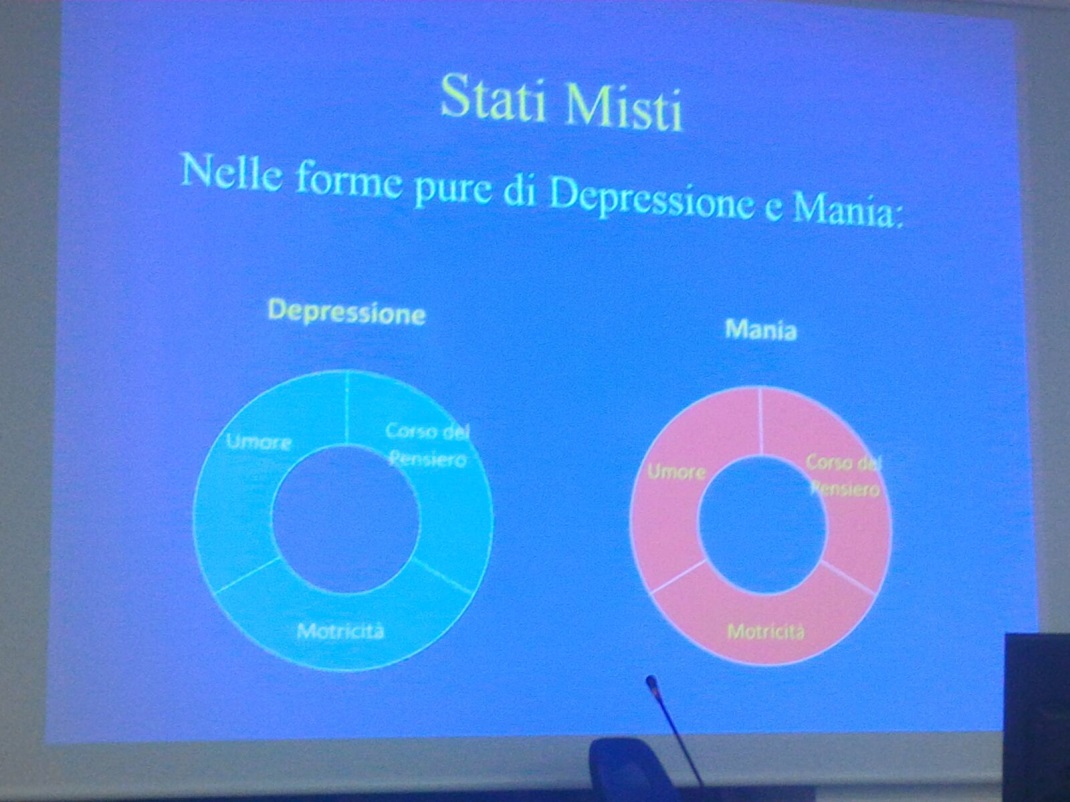
\includegraphics[width=0.9\textwidth]{02/image10.jpeg}
\end{figure}

N\emph{egli stati misti}, invece, \emph{due dei tre elementi sono
concordi per polarità, mentre uno ha polarità opposta}, per cui vi sono
essenzialmente 6 combinazioni principali:


\begin{table}
%\caption{Please write your table caption here}
\begin{tabular}{p{0.5\textwidth}p{0.5\textwidth}}

Mania depressiva		&	Tono dell’umore depresso, ma con ideazione e motilità aumentate \\
Mania acinetica		&	Tono dell’umore aumentato, ideazione accelerata, ma riduzione della motilità  \\
Depressione con fuga delle idee	&	Tono dell’umore depresso, motilità ridotta, ma ideazione aumentata \\
Mania improduttiva	&	Tono dell’umore elevato, motilità aumentata, ma ideazione ridotta \\
Depressione Agitata	&	Tono dell’umore depresso, ideazione inibita, ma motilità aumentata \\
Stupor Maniacale		&	Tono dell’umore elevato,  ma motilità ed ideazione ridotte \\

\noalign{\smallskip}\hline\noalign{\smallskip}
\end{tabular}
\end{table}


\begin{figure}[!ht]
\centering
	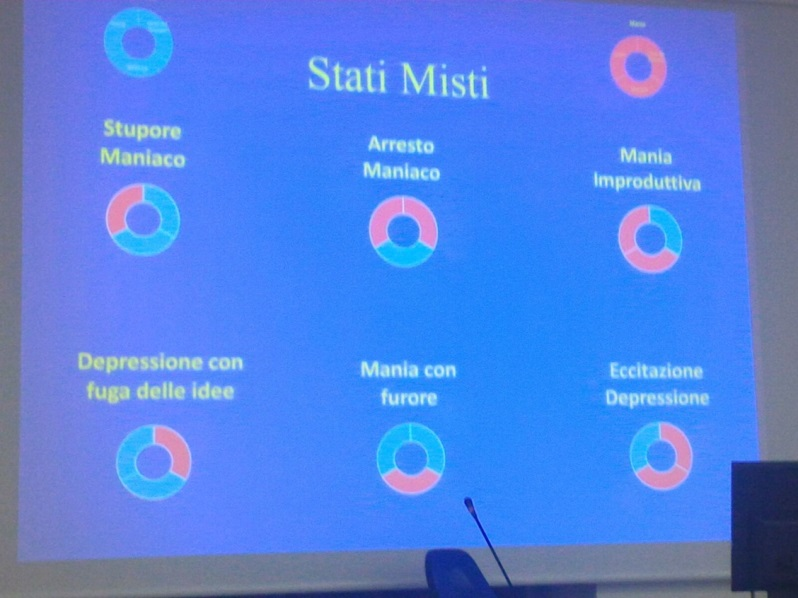
\includegraphics[width=0.9\textwidth]{02/image11.jpeg}
\end{figure}

Gli stati misti possono poi essere suddivisi in \textbf{STABILI} ed
\textbf{INSTABILI} in base alla \emph{comparsa di variazioni
persistenti} (stabili) \emph{o di viraggi rapidamente alternantisi}
(instabili) \emph{a carico dell'affettività}, \emph{dell'energia vitale
e della risonanza affettiva}.

Spesso si possono poi avere delle \textbf{alterazioni del bioritmo},
come disturbi del sonno o variazioni diurne o quasi circadiane dei
parametri prima descritti.

Forme particolari di disturbi bipolari sono poi lo \textbf{stato misto
maniaco-depressivo}, che si caratterizza per la presenza di
\emph{fenomeni dispercettivi}, \emph{idee deliranti}, \emph{alterazioni
della coscienza spesso indistinguibili da quelli della demenza praecox},
ed il \textbf{disturbo bipolare a cicli rapidi}, caratterizzato dalla
presenza di \emph{almeno 4 episodi di alterazione dell'umore nei 12 mesi
precedenti}, che soddisfano i criteri per un episodio depressivo
maggiore, maniacale, misto o ipomaniacale, i quali sono \emph{demarcati
da una remissione parziale o completa per almeno 2 mesi}, o da un
viraggio verso un episodio di opposta polarità.
\end{itemize}

\textbf{Di seguito una serie di casi clinici esemplificativi dei
disturbi visti:}

\emph{Caso clinico 1:}

Pz che diceva di essere ``l'anti-cristo'' (usando questo termine
intendendo di essere il ``secondo cristo'', quindi un salvatore del
mondo - mania), ma dopo poche ore lo ritrovavamo che affermava di essere
incapace e indegno \textbf{stato misto instabile}.

\emph{Caso clinico 2:}

Pz ricoverata, 38 anni, che è convinta di essere la Madonna. Dice che da
piccola era stata ricoverata in pediatria e che di fianco a lei c'era
una bambina con un cappotto rosso e che lei non ha più visto, e afferma
che: ``non so se è perché l'hanno buttata dalla finestra o se perché mi
hanno buttato dalla finestra. Però penso di averla ritrovata..'' e
indica la sua vicina di letto (ma non è possibile dato che ha 20 anni in
più di lei). La pz poi di notte vaga per il reparto, presa da frenesia,
ma alla mattina non lo ricorda, non ricorda nemmeno di aver preso le
gocce alla sera. Lei è convita che questo sia un effetto collaterale dei
farmaci (acatisia in effetti può esserlo) ma non è possibile che si
manifesti solo di sera!

Da questo si è capito che, probabilmente, dato che lei tende ad
oscillare nell'umore, di notte è agitata e si trova in uno stato molto
particolare, un po' come soggetti anziani con demenza che vanno incontro
a confusione soprattutto di notte. La pz ha queste alterazioni molto
particolari: se non si fa attenzione si potrebbe sbagliare la diagnosi,
pensando a schizofrenia o a un quadro di compromissione cerebrale grave.

\emph{Caso clinico 3:}

Signora di 50 anni, che vestiva sempre in grigio o nero. Un giorno si
presenta vestita in modo eccentrico (camicia hawaiana, gonna fucsia,
cappellino, infradito) era cambiata la fase di malattia. Afferma che
sarebbe atterato un elicottero e che l'avrebbero portata in
spiaggia\ldots{}

Questo per dire che per capire se il pz è nella fase maniacale non c'è
particolarmente bisogno di parlare con lui\ldots{}è evidente!

\emph{Caso clinico 4:} in cui pz si presenta in day hospital vestito
come nativo indiano, con penna in testa e lenzuolo attorno alla
vita\ldots{}e nella schiena era pieno di tagli perché si era grattato
con un coltello!

\emph{Caso clinico 5:} il paziente era indeciso se alle olimpiadi fare i
100 m o baseball, e in questo dissidio faceva 10 min di corsa e 10
giocando con la palla\ldots{}

\emph{Caso clinico 6:} il paziente disegnava su fogli un progetto per un
macchinario in grado di spostare la casa da un punto ad un altro perché
era convinto che spostando la casa di 50 metri sarebbe stata più bella
la locazione.

\subsubsection{Distimia}

Mentre nella depressione maggiore e nel disturbo bipolare le fasi di
malattia durano qualche mese (5-6 mesi), poi abbiamo un ritorno
all'eutimia e poi di nuovo un altro episodio; nella distimia invece
abbiamo un disturbo che ha una durata molto più lunga.

È una delle forme di \emph{disturbo dell'umore ad andamento cronico},
anch'essa piuttosto frequente, che secondo i criteri del DSM-IV si
contraddistingue per la \emph{presenza di umore depresso per quasi tutto
il giorno, quasi ogni giorno, per un periodo di almeno due anni},
associato a \emph{due o più dei seguenti sintomi}:

\begin{itemize}
\item
  \textbf{Scarso appetito} o \textbf{iperfagia};
\item
  \textbf{Insonnia} o \textbf{ipersonnia};
\item
  \textbf{Scarsa energia} o \textbf{astenia};
\item
  \textbf{Bassa autostima};
\item
  \textbf{Difficoltà a concentrarsi o nel prendere decisioni};
\item
  \textbf{Sentimenti di disperazione}.
\end{itemize}

Inoltre, durante i due anni di malattia, il soggetto \emph{non deve mai
essere stato privo di sintomi per più di 2 mesi}, e durante il periodo
di malattia \emph{non si devono avere episodi depressivi maggiori
(}tende ad oscillare in prossimità dell'umore normale), così come non
deve essere \emph{mai stato presente un episodio maniacale, misto o
ipomaniacale}, né sono mai stati soddisfatti i criteri per il disturbo
ciclotimico, ed i sintomi devono causare un disagio clinicamente
significativo o una compromissione del funzionamento sociale, lavorativo
o di altre aree importanti.

Bisogna fare quindi molta attenzione, perché prima dell'insorgere del
disturbo distimico può esserci stato un episodio depressivo maggiore,
purché seguito da una remissione totale (cioè senza sintomi per almeno 2
mesi); inoltre, dopo i primi 2 anni (1 solo anno per bambini o
adolescenti) di disturbo distimico possono esserci degli episodi
depressivi maggiori sovrapposti, condizione nota come
``\textbf{\emph{depressione doppia}}'', e la diagnosi viene posta a
seguito del soddisfacimento dei criteri per la depressione maggiore in
paziente già affetto da disturbo distimico. In questo caso, il DSM
raccomanda di riportare se si tratta di una forma ad \emph{esordio
precoce} (sotto i 21 anni), ad \emph{esordio tardivo} (dopo i 21 anni) o
se sono presenti manifestazioni \emph{psicotiche}.

\subsubsection{Ciclotimia}

E\textbf{'}un disturbo che ha sempre una durata estremamente lunga,
almeno 2 anni in cui il soggetto oscilla sia sul versante depressivo,
lieve, sia sul versante ipomaniacale, sfumato, e per due anni continua
in questa oscillazione.

\emph{\textbf{Alcune domande d'esame}} potrebbero essere:

\begin{itemize}
\item[1.]
  quante forme depressive conoscete?
\item[2.]
  Quanti disturbi bipolari conoscete?
\item[3.]
  Un paziente con disturbo bipolare che possibilità ha di avere una vita
  normale?
\end{itemize}

\documentclass[]{article}
\usepackage{lmodern}
\usepackage{amssymb,amsmath}
\usepackage{ifxetex,ifluatex}
\usepackage{fixltx2e} % provides \textsubscript
\ifnum 0\ifxetex 1\fi\ifluatex 1\fi=0 % if pdftex
  \usepackage[T1]{fontenc}
  \usepackage[utf8]{inputenc}
\else % if luatex or xelatex
  \ifxetex
    \usepackage{mathspec}
  \else
    \usepackage{fontspec}
  \fi
  \defaultfontfeatures{Ligatures=TeX,Scale=MatchLowercase}
\fi
% use upquote if available, for straight quotes in verbatim environments
\IfFileExists{upquote.sty}{\usepackage{upquote}}{}
% use microtype if available
\IfFileExists{microtype.sty}{%
\usepackage{microtype}
\UseMicrotypeSet[protrusion]{basicmath} % disable protrusion for tt fonts
}{}
\usepackage[unicode=true]{hyperref}
\hypersetup{
            pdfborder={0 0 0},
            breaklinks=true}
\urlstyle{same}  % don't use monospace font for urls
\usepackage{longtable,booktabs}
% Fix footnotes in tables (requires footnote package)
\IfFileExists{footnote.sty}{\usepackage{footnote}\makesavenoteenv{long table}}{}
\usepackage{graphicx,grffile}
\makeatletter
\def\maxwidth{\ifdim\Gin@nat@width>\linewidth\linewidth\else\Gin@nat@width\fi}
\def\maxheight{\ifdim\Gin@nat@height>\textheight\textheight\else\Gin@nat@height\fi}
\makeatother
% Scale images if necessary, so that they will not overflow the page
% margins by default, and it is still possible to overwrite the defaults
% using explicit options in \includegraphics[width, height, ...]{}
\setkeys{Gin}{width=\maxwidth,height=\maxheight,keepaspectratio}
\IfFileExists{parskip.sty}{%
\usepackage{parskip}
}{% else
\setlength{\parindent}{0pt}
\setlength{\parskip}{6pt plus 2pt minus 1pt}
}
\setlength{\emergencystretch}{3em}  % prevent overfull lines
\providecommand{\tightlist}{%
  \setlength{\itemsep}{0pt}\setlength{\parskip}{0pt}}
\setcounter{secnumdepth}{0}
% Redefines (sub)paragraphs to behave more like sections
\ifx\paragraph\undefined\else
\let\oldparagraph\paragraph
\renewcommand{\paragraph}[1]{\oldparagraph{#1}\mbox{}}
\fi
\ifx\subparagraph\undefined\else
\let\oldsubparagraph\subparagraph
\renewcommand{\subparagraph}[1]{\oldsubparagraph{#1}\mbox{}}
\fi

% set default figure placement to htbp
\makeatletter
\def\fps@figure{htbp}
\makeatother


\date{}

\begin{document}

\textbf{\emph{TERAPIA DEI DISTURBI DELL'UMORE:}}

Il \textbf{trattamento dei disturbi} dell'umore differisce in base al
tipo di disturbo che interessa il paziente, nonché in base alla sua
gravità, alle condizioni cliniche del paziente e dalla presentazione in
acuto o in cronico. Durante i trattamenti di emergenza è fondamentale
garantire la sicurezza del paziente valutando se vi siano le condizioni
per un trattamento ambulatoriale o se sia più opportuno il ricovero in
regime di day hospital o l'ospedalizzazione, anche mediante TSO, e
successivamente si può procedere con un'adeguata terapia farmacologica e
psicologica.

\textbf{\emph{TRATTAMENTO DEGLI EPISODI DEPRESSIVI:}}

\textbf{\emph{LINEE GUIDA:}}

\emph{\emph{CASO CLINICO: Nella fine degli anni '80 negli Stati Uniti un
nefrologo, dottor Osheroff, che dal punto di vista professionale ha
avuto un buon successo: ha un clinica importante, mentre dal punto di
vista sentimentale è al terzo matrimonio e mantiene in affido due figli,
avuti nei precedenti matrimoni.}}

\emph{Ad un certo punto comincia ad avere una sintomatologia depressiva
lieve, con una componente ansiosa piuttosto sfumata: chiede aiuto ad un
collega che gli prescrive una terapia farmacologica e una psicoterapia.
}

\emph{Fa la terapia in modo discontinuo, e dopo alcuni mesi si ritrova
nella situazione iniziale.}

\emph{Allora il suo collega gli propone un periodo di ricovero di alcune
settimane, così da poter tornare in seguito a fare la sua vita. Viene
ricoverato nel centro privato più prestigioso degli USA, dove la cura
fondamentale è la \textbf{psicanalisi}. Dopo il primo colloquio comincia
una terapia che consiste in quattro sedute a settimana, senza apporto
farmacologico.}

\emph{Dopo alcune settimane la situazione è peggiorata: non dorme, è
molto agitato, comincia a perdere di peso. Quando la moglie lo va a
trovare lui è preoccupato: la moglie, che lo è altrettanto, chiama un
collega psichiatra per confrontarsi sulla situazione. La clinica decide,
viste le perplessità, di riunirsi con il professionista esterno per
giudicare e poi decidere insieme il da farsi. Il responso della Case
Conference: ``la terapia è quella giusta, si tratta solo di aspettare
tempo''.}

\emph{Passano fino a sette mesi ed il paziente sta sempre peggio, è
dimagrito di 20kg, ha insonnia totale e compaiono anche deliri.}

\emph{La moglie allora dedice di trasferirlo da un'altra parte, in una
struttura che agisce con trattamento opposto, basato sull'approccio
farmacologico.}

\emph{Già dopo 2 settimane compaiono i primi miglioramenti. Trascorso un
mese e mezzo nella nuova clinica il paziente sta bene, è dimesso con
terapia da continuare da casa e altre sedute di psicoterapia.}

\emph{Tornato a casa dopo nove mesi il dottore, con centro di dialisi
chiuso e figli tornati dalla moglie, decide di fare causa alla prima
clinica (quella che basava l'approccio sulla psicoanalisi): chiede un
risarcimento danni, visto che non lo aveva curato per sette mesi.}

\emph{Il giudice ha chiesto a quelli della struttura i dati che avevano
a disposizione, per dimostrare che la terapia del dottore aveva dato
buoni risultati.}

\emph{Il problema è che gli psicanalisti hanno come posizione teorica il
fatto che la loro terapia non è misurabile, perchè quello che diventa
curativo è il rapporto che si instaura tra loro e il paziente, e quindi
è diverso da paziente a paziente; ciò diventa irripetibile, quindi
difficilmente misurabile.}

\emph{Per esempio esistono studi di meta analisi in cui si mettono
insieme tutti gli studi effettuati con la stessa metodologia, arrivando
ad avere risultati su casistiche molto ampie (anche 5000 pazienti).}

\emph{Perciò la clinica ha risposto che di risultati non ne avevano,
perchè per loro il metodo scientifico è inapplicabile alla psicanalisi.}

\emph{Il giudice prende atto e interpella la seconda clinica che ha
eseguito l'approccio farmacologico: loro hanno tutte le prove che
servono, perchè gli antidepressivi già dagli anni '60 erano usati e
dimostrati nella loro efficacia.}

\emph{Alla fine il giudice fondò la sua sentenza sul presunto silenzio
da parte della prima clinca (quella psicanalitica), riguardo gli effetti
postivi, scientificamente testati, della seconda clinca (quella con
trattamento farmacologico). Avrebbero dovuto avvisare il paziente della
possibile alternativa.}

Non a caso che le prime linee guida, e quindi l' evidence based medecine
in ambito psichiatrico, sono uscite circa una decina di anni dopo,
proprio sul trattamento della depressione maggiore, per poi in seguito
uscire per tutti i disturbi.

Su cosa si basa l'evidence based medecine?

Sono le metanalisi, degli studi clinici randomizzati in doppio cieco, ad
essere le più pesanti dal punto di vista dell'evidenza. Ci sono due
fattori fondamentali che deve avere il paziente per essere idoneo a uno
studio:

\begin{itemize}
\item
  non rimanere incinta durante la terapia: Abbiamo dati di trattamenti
  con antidepressivi in gravidanza, anche nel primo trimestre, che
  superano le 20000 pazienti, ma non sono stati mai approvati: andando a
  vedere le indicazioni del FDA (food and drug administration), non
  c'erano fino a pochi anni fa farmaci per il trattamento delle donne in
  gravidanza.
\item
  non essere a rischio di suicidio: se questo dovesse avvenire mentre
  assume un farmaco sperimentale, questo viene immediatamente
  abbandonato (ad esempio è successo a un farmaco della Pfizer per l'
  ipercolesterolemia).
\end{itemize}

Il problema che sorge da tutto ciò è il seguente: se non è possibile
mettere questi tipi di pazienti negli studi randomizzati, ma il medico
si trova a dover trattare uno di questi, non può rifiutarsi di trattarlo
perchè non sono presenti linee guida a riguardo. Risulta chiaro come sia
necessario agire ben oltre quello che è fornito dai dati statistici,
qualora, per necessità clinica, debba relazionarmi con una paziente
depressa incinta/ a rischio suicidio.

\textbf{Dunque è per necessità clinica che le linee guide hanno dovuto
essere superate}. Quindi nelle condizioni cliniche rilevanti, in cui non
c'è uno studio che abbia trattato ad esempio un paziente a rischio di
suicidio, vale l'esperienza clinica.

Come esempio:

\begin{itemize}
\item
  \emph{nei pazienti più gravi, in genere ricoverati, il fatto che io
  debba usare un triciclico non deriva dagli studi randomizzati, ma
  deriva esclusivamente dall'esperienza clinica.}
\item
  \emph{Nelle donne gravide: È bene precisare che farmaci
  anti-depressivi si usano anche nei primi trimestri di gravidanza e
  sono compatibili con l'allattamento, non perchè non passi (tutti i
  farmaci passano nella placenta e nel latte), ma la percentuale è
  davvero molto bassa. Qualche gruppo americano ha fatto anche un
  prelievo ai bambini ed era indosabile nel plasma.}
\end{itemize}

Di LINEE GUIDA ce ne sono tante, canadese, neozelandese, inglese ecc,
quelle forse migliori sono della \emph{American Psychiatric
Association}, perchè sono più approfondite, hanno più pagine su farmaci
e effetti collaterali. Quelle europee sono meno dettagliate, vi dicono
le indicazioni generiche per un determinato disturbo senza entrare nel
merito del singolo trattamento, quindi più in termini di scelta e durata
della terapia.

Per capire meglio, ad esempio le linee USA indicano per un trattamento i
possibili interazioni, effetti collaterali, mentre le europee non
considerano questi aspetti e danno linee di principio, infatti sono di
10-12 pagine contro le circa 100 delle altre.

\textbf{INDICATORI NELLA SCELTA DEL TRATTAMENTO:}

Sono la Gravità e la Durata della depressione:

\begin{enumerate}
\def\labelenumi{\arabic{enumi}.}
\item
  \textbf{La GRAVITÀ della depressione: }

  Per il DSM (Il Manuale Diagnostico e Statistico dei Disturbi Mentali)
  la \textbf{gravità dei sintomi} è espressa semplicemente contando il
  numero dei sintomi:
\end{enumerate}

\begin{itemize}
\item
  lieve= 5,
\item
  moderata=7,
\item
  grave se maggiore di 7,
\item
  molto grave se ha sintomi psicotici, quindi depressione delirante.

  Questo è un criterio un pò grossolano, basta che ne abbia uno, ma
  molto intense, per avere un quadro più grave rispetto ad un'altro:
  quindi tenere conto solo del numero, ma non della gravità, è
  estremamente impreciso.

  La depressione breve ricorrente ha i 5 sintomi, ha una durata molto
  più breve ed è, ad esempio, una forma con rischio di suicidio molto
  più elevato.

  Il ricovero dovrebbe scattare nelle forme deliranti, ad alto rischio
  di suicidio, o in forme molto complicate da gestire, ad esempio un
  anziano con problemi internistici.
\end{itemize}

\begin{itemize}
\item
  Per pazienti con una GRAVITÀ LIEVE le possibilità di trattamento sono
  molte:
\end{itemize}

Messa in evidenza in un grafico di meta analisi \textbf{l'efficacia
degli antidepressivi in relazione alla gravità della depressione,}
pubblicato su Jama.

Immaginiamo un grafico con\textbf{:}

In ordinate è espresso il cambiamento rispetto a prima del trattamento

In ascissa si trova la misurazione della gravità della depressione con
la scala di Hamilton. È da tenere presente che quando è svolto uno
studio su un nuovo farmaco in genere sono inclusi pz che abbiano almeno
18. Questo è il cambiamento che è possibile ottenere prima e dopo;
quindi se è ottenuto 12 vuol dire che c'è stata una riduzione di 12
punti della scala di Hamilton.

\textbf{Conclusioni ottenute:}

È stabilito a 25 il punteggio di gravità della sintomatologia
depressiva, misurata con il famoso Hamilton, che discrimina tra
superiorità del trattamento con farmaci rispetto al placebo.

Al di sotto di quel livello placebo e farmaci danno lo stesso risultato,
mentre al di sopra di 25 il farmaco è decisamente più efficace.

Diversi studi dimostrano che un punteggio inferiore a 23, quindi siamo
nella fascia sotto quel limite, è posseduto dai 2/3 (75\%) dei pazienti.

Quindi possiamo somministrare:

\begin{itemize}
\item
  PLACEBO: \textbf{Come dare un placebo al paziente:} È presa in esame
  una di quelle donne che tra i 15 e 50 anni vanno dallo psichiatra: ha
  una depressione di 24; si dimostra di poterle dare qualunque
  trattamento, ma come si fa a darle un placebo?

  Si potrebbe dare un antidepressivo, ma un conto è dirle che funziona
  come antidepressivo ed un conto è dire che funziona come placebo.
  Infatti, dicendole che è un placebo, praticamente non si riesce a
  somministrare un placebo, questo è difficile da applicare in
  psichiatria.

  È possibile allora dire alla paziente che il farmaco che assume non ha
  nessun effetto a livello farmacologico, ma attiva le stesse aree a
  livello cerebrale del farmaco vero e proprio, questo è stato il metodo
  per somministrare il placebo.

  Un americano lo ha fatto nel colon irritabile, il risultato è che
  l'effetto sulla patologia è analogo tra antiinfiammatorio e placebo.

  Prendendstudio sull'agopuntura per meglio descrivere l'entità
  dell'effetto placebo.

  Lo studio è sul trattamento di emicrania, cefalea muscolo tensiva,
  dolore lombare cronico, randomizzati. La usual care riceve visita
  medica più analgesico, l'altro gruppo è trattato con agopuntura:
  l'effetto è il medesimo.

  Inoltre nell'ambito della stessa agopuntura, far inserire gli aghi a
  un esperto agopunturista in punti ben determinati, oppure a una
  persona qualunque, purchè gli si insegni il metodo per inserirli,
  dimostra che il miglioramento del dolore è esattamente lo stesso.

  Se l'analgesico viene presentato dicendo che è il migliore farmaco,
  questo ha un effetto assolutamente migliore. Se lo stesso farmaco è
  somministrato endovena senza essere enfatizzato al paziente l'effetto
  analgesico scompare. Addirutta ci sono studi sul colore del farmaco
  placebo: più colorato è, meglio è efficace.

  In conclusione: l'aspettativa che ha il paziente assume un ruolo
  determinante nell'efficacia di un trattamento, sia che questo sia
  farmacologico, sia che sia un placebo.

  Quindi che il placebo sia una sostanza inerte, non è del tutto vero:
  il placebo modifica le aree cerebrali, cioè le stesse che modificano i
  farmaci; lo stesso fa la psicoterapia.
\end{itemize}

\begin{itemize}
\item
  TERAPIA FARMACOLOGICA
\item
  TERAPIA PSICOTERAPEUTICA, di quest'ultime è dimostrata l'efficacia
  solo se ad orientamento cognitivo comportamentale.

  Il punto cardine di quest'ultime è: ``Io ho appreso qualcosa di errato
  che devo disapprendere''.

  Esempio: \emph{non avere sicurezza, non valere nulla, temere che tutto
  debba andare male;} è uno stile cognitivo che ho imparato e che devo
  disimparare.

  \textbf{Man mano che aumenta la gravità la psicoterapia perde
  efficacia,} la farmacoterapia diviene allora un'indicazione
  fondamentale.
\end{itemize}

È chiaro che bisogna ricordare quello che dicevano gli inglesi:
\textbf{tanto più il disturbo è lieve e breve, tanto più risponde alla
aspettativa di un miglioramento, qualunque esso sia}. L'agopuntura,
l'omeopatia, la terapia di rilassamento. Per l'omeopatia è uscito anche
un articolo sull'ansia assolutamento sovrapponibile al placebo.

\textbf{I triciclici in genere servono per le forme più gravi e il
placebo per quelle più lievi}. L'efficacia sale per tutti e tre i
trattamenti, placebo compreso, dagli anni '80 agli anni 2000.

Dagli anni '80 agli anni 2000 la risposta al trattamento è aumentata;
nel placebo va dal 20 al 30\%, mentre per i serotoninergici e
tricliclici dal 40 al 50\%.

\emph{\emph{Quando uno psichiatra decide di somministrare a un paziente
con depressione lieve un trattamento farmacologico, deve tenere presente
che questo è analogo al placebo o al trattamento psicologico.}} Quindi
non c'è differenza di mortalità tra placebo e un farmaco normale nelle
forme lievi, il placebo equivale alla psicoterapia.

A livello economico è più costoso dare un placebo che un farmaco.
Infatti è da tenere presente che un'ora di psicoterapia costa 80-100
euro, mentre il farmaco antidepressivo più prescritto costa 6 euro al
mese (quindi con 100 euro è possibile fare 16 mesi di terapia
farmacologica).

Dal punto di vista di uno psicoterapeuta è importante che abbia la
consapevolezza di poter guarire l'episodio depressivo soltanto se questo
non è grave (può farlo, perchè in quel caso tutti i trattamenti sono
equivalent). Quello che invece lo psichiatra può fare non è pensare di
risolvere il conflitto alla base della depressione maggiore o del
disturbo bipolare, ma fare in modo che il paziente non abbia più
ricadute.

È possibile trattare l'episodio e aumentare la consapevolezza,
soprattutto nei bipolari, che è presente un disturbo da gestire, che
bisogna seguire la terapia con regolarità e adottare un certo stile di
vita.

Questo non è secondario, perchè nel disturbo bipolare i pazienti che
seguono il trattamento e le visite hanno un rischio di suicidio
dimezzato rispetto a quelli che non lo fanno: per cui lavorare su questo
è importante, perchè è ridotto il tasso di suicidio del 50\%.

\begin{itemize}
\item
  Per pazienti con GRAVITÀ ELEVATISSIMA:
\end{itemize}

\begin{itemize}
\item
  L'ELETTROSHOCK è stato scoperto da un neurologo italiano negli anni
  30, Ugo Cerletti. I farmaci esistono dagli anni '50, prima non si
  sapeva cosa fare.

  \emph{Il professore cita, per comprendere pienamente la difficoltà dei
  trattamenti psichiatrici prima dell'avvento dei farmaci, ``Le libere
  donne di Magliano'' e ``Per le antiche scale'', libri di Mario Tobino,
  uno psichiatra che ha lavorato nell'ospedale di Lucca.}

  \emph{Egli descrive i pazienti che vengono inviati alle ``alghe'', una
  stanza piena di alghe dove il paziente veniva messo nudo, per evitare
  che si potesse fare del male.}

  \emph{Prima del trattamento farmacologico si ricorreva a:
  elettroshock, shock insulinico, shock cardiazolico, bagni con shock
  termico.}

  \textbf{L'elettroshock è il trattamento più efficace in depressioni di
  gravità elevatissima}, è lo stesso concetto applicato nella
  cardioversione, annullare tutti i potenziali di membrana con una
  corrente, cosicchè i neuroni ripartano in condizioni normali.

  Ancora oggi ci sono pazienti lo richiedono, perchè la loro descrizione
  è questa: ``Entravo con nessun altro pensiero, se non quello di farla
  finita, ed uscivo che stavo bene''.

  È eseguito in anestesia generale, si vede la crisi epilettica solo per
  il movimento del piede, il paziente è curarizzato. È utile solo in
  questi casi, non ha altre indicazioni, farlo senza è una malpractice:
  oggi è praticamente limitato ai gravi rischi di suicidio.
\end{itemize}

\begin{itemize}
\item
  Per pazienti con DEPRESSIONE DELIRANTE:
\end{itemize}

\begin{itemize}
\item
  ANTIDEPRESSIVI con associati ANTISPSICOTICI sono raccomandati, se è
  presente sintomatologia delirante.
\end{itemize}

\begin{itemize}
\item
  Per pazienti con DEPRESSIONE associata a PATOLOGIA CORONARICA:

  La depressione rappresenta un aumento di rischio di mortalità in
  pazienti con paotlogia coronarica.

  Se prendiamo in considerazione pazienti con sintomi depresssivi
  (pazienti sotto soglia, in cui il quadro clinico depressivo non
  raggiunge la soglia della diagnosi), perchè mai andrebbero trattati?
  \textbf{\emph{Perchè con sintomi depressivi si ha un rischio 1.7 volte
  maggiore di morire, rispetto ad un altro paziente con la stessa
  patologia cardiaca (non depresso).}}

  Più la depressione è lunga, più questo moltiplicatore del rischio
  aumenta:

  2 se meno di 6 mesi
\end{itemize}

\begin{quote}
2.6 se più di 6 mesi

Diventa quindi importante anche ciò che è sotto soglia, perchè ha
un'influenza infausta sul decorso di tutte le patologie, soprattutto
quelle cardiovascolari.

La depressione, anche molto sfumata, ha un effetto nefasto sul decorso
di tutti i disturbi medici e in particolare le malattie cardiovascolari.

\emph{Viene mostrato il risultato di uno studio pubblicato su JAMA,
relativo alla probabilità di morte dei pazienti post infarto, con e
senza un trattamento psicoterapeutico a confronto.}

Sono più di 1000 pazienti che hanno avuto un infarto. Valutando le linee
guida, non è detto di doverli trattare con la terapia farmacologia;
quindi è possibile approcciarli tranquillamente con la terapia
psicologica.

Questo studio ha un braccio in cui i pazienti hanno un trattamento
psicologico e un braccio in cui i pazienti hanno un trattamento
farmacologico.

Il gruppo di controllo è definito \emph{usual care}. In pratica il
paziente è sottoposto a visita cardiologica, fa un colloquio sulle
condizioni cardiache e in parte anche sullo stile di vita.

L'altro gruppo oltre alla visita cardiologica riceve una psicoterapia
cognitivo comportamentale.

I due strumenti di valutazione:
\end{quote}

\begin{itemize}
\item
  (BDI) auto-somministrato, è il paziente che lo compila\emph{: In
  genere l'autovalutazione tende a dare un disturbo un pò più grave,
  cioè tende a sovra-stimare la gravità}
\item
  HRSD è il medico che lo compila: \emph{mentre la valutazione di un
  osservatore tende a ridurre questa gravità}
\end{itemize}

\begin{quote}
Il risulato è che si si ha un miglioramento in entrambi i casi della
depressione ed è qui sorge il problema: esistono due trattamenti che,
secondo le linee guida, sono entrambi efficaci per le depressioni lievi.
Però i farmaci riducono la mortalità e i nuovi rischi di infarto, mentre
la psicoterapia, pur essendo efficace nella depressione non agisce sul
versante cardiovascolare.

Allora perche gli antidepressivi funzionano anche sul cuore? Lo si deve
al fatto che loro sono anche anti-aggreganti piastrinici? Non esiste
ancora risposta a questo quesito.

\emph{Cochrane}, ente privato che si occupa dei problemi sanitari (in
genere fa delle metanalisi o revisioni) ha effettuato uno studio a
riguardo. Gli studi di questa agenzia hanno 3 destinatari:
\end{quote}

\begin{itemize}
\item
  pazienti
\item
  medici
\item
  amministratori sanitari
\end{itemize}

\begin{quote}
\textbf{Si è concluso che gli interventi psicologici nel loro complesso
non hanno mostrato efficacia sulla mortalità totale cardiaca}, benchè
mostrino una riduzione nei livelli di ansia e depressione nei pazienti
con cardiopatia coronarica; questa è in parte la spiegazione del perchè
anche con depressione subliminare vanno trattati.
\end{quote}

\begin{enumerate}
\def\labelenumi{\arabic{enumi}.}
\item
  E' introdotto oltre al criterio di gravità anche quello di
  \textbf{DURATA}:

  Il trattamento farmacologico antidepressivo, ovviamente rispetto al
  placebo, è indicato nei casi particolarmente gravi oppure di durata
  prolungata. Quindi un caso di non particolare gravità, ma di durata
  prolungata, può trovare questa indicazione: è il caso della
  depressione sotto soglia, anche detta minore.
\end{enumerate}

\textbf{\emph{FARMACI ANTIDEPRESSIVI:}}

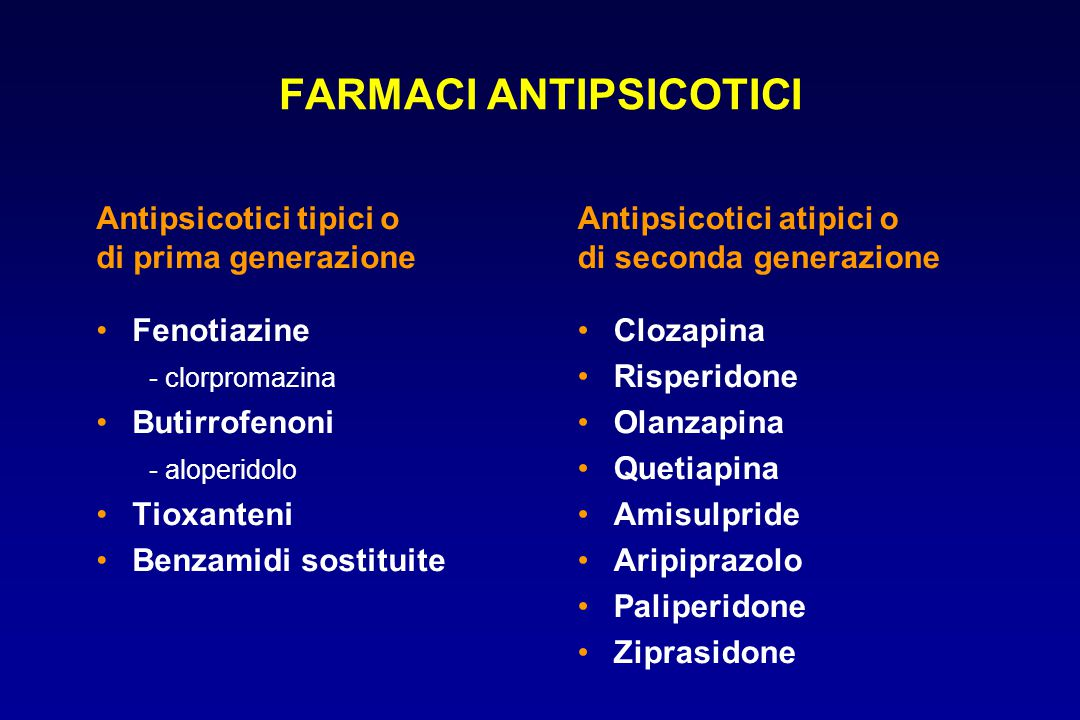
\includegraphics[width=4.96389in,height=3.02431in]{media/image1.jpeg}

Per gli \textbf{episodi} \textbf{depressivi}, il trattamento si basa
sull'uso dei \emph{farmaci antidepressivi} e, nei casi più gravi, della
\emph{TEC} (Terapia Elettro-Convulsivante); tra gli antidepressivi sono
disponibili diverse classi di farmaci, come gli \textbf{SSRI} (Inibitori
Selettivi della Ricaptazione della Serotonina), gli
\textbf{antidepressivi tetraciclici} e \textbf{triciclici}
(\textbf{TCA}), gli \textbf{IMAO} (Inibitori delle Monoammino-Ossidasi),
gli \textbf{SNRI} (Inibitori della Ricaptazione della Serotonina e della
Noradrenalina), i \textbf{NARI} (Inibitori Selettivi della Ricaptazione
della Noradrenalina), gli agonisti melatoninergici ed i \textbf{NaSSA}
(Antidepressivi noradrenergici e serotoninergici specifici).

\begin{itemize}
\item
  \emph{MECCANISMO:}
\end{itemize}

\begin{itemize}
\item
  \textbf{Blocco del reuptake}:

  \begin{itemize}
  \item
    Serotonina (SSRI; SNRI)
  \item
    Noradrenalina (TCA;NARI)
  \end{itemize}
\end{itemize}

\textbf{1\emph{.ANTIDEPRESSIVI TRICILICI (TCA):}}

\emph{\emph{Usi Clinici:}}

I farmaci antidepressivi triciclici e tetraciclici (TCA) sono
generalmente riservati ai casi depressivi che \emph{non rispondono né
agli SSRI né agli SNRI}.

In realtà sono farmaci di prima scelta per il trattamento delle forme
depressive di maggiore gravità: con \emph{caratteristiche melanconiche}
o con \emph{rallentamento motorio}; infatti quando prevalgono
l'inibizione ed il rallentamento è bene ricorrere a TCA ad azione
attivante, come la \textbf{desipramina} e la \textbf{nortriptilina}.

Per le forme depressive \emph{con ansia ed agitazione} si utilizzano
preferibilmente l'\textbf{amitriptilina}, l'\textbf{imipramina} e la
\textbf{trimipramina}, che sono farmaci con marcata attività sedativa.

Alcuni farmaci TCA, inoltre si sono dimostrati utili anche nel
trattamento di eventuali \emph{disturbi psichiatrici associati alla
depressione}, ad esempio:

\begin{itemize}
\item
  la \textbf{clomipramina} è utile per i pazienti depressi che soffrono
  anche di \emph{disturbo ossessivo} c\emph{ompulsivo}. infatti il
  disturbo ossessivo-compulsivo risponde esclusivamente ai farmaci
  serotoninergici o pro-serotoninergici, infatti con altri farmaci, per
  esempio ammine secondarie, non avviene la terapia. Tant'è che la
  clomipramina soltanto, perchè è aggiunto un cloro, è uno dei maggior
  farmaci che agisce sul sistema della serotonina. Dando altri
  triciclici non si nota nessun miglioramento; quindi solo modificando
  appena la struttura è ottenuta una diversa efficacia e tollerabilità.
\end{itemize}

\begin{itemize}
\item
  mentre l'\textbf{imipramina} è efficace anche contro i sintomi del
  \emph{disturbo di panico.}
\end{itemize}

\emph{\emph{Effetti collaterali:}}

Gli \emph{effetti collaterali} dei TCA sono essenzialmente dovuti alla
loro azione anticolinergica, antistaminica ed adrenolitica, e sono
generalmente più intensi nelle prime due settimane di cura, con:
ipotensione ortostatica, tachicardia riflessa, turbe del ritmo e della
conduzione cardiaca, tremori, atassia, discinesie, deficit della memoria
e della concentrazione, sedazione e confusione (negli anziani), visione
offuscata, vertigini, abbassamento della soglia convulsiva, alterazioni
della libido, impotenza, ritenzione urinaria e, soprattutto nelle
terapie a lungo termine, aumento ponderale, stipsi, xerostomia ed
iperidrosi.

In particolare:

\begin{itemize}
\item
  \emph{Anti-alfa 1} → Il tono delle arteriole dipende molto dalle alfa
  1, infatti i nostri pz hanno ipotensione ortostatica (in un giovane si
  annebbia la vista, mentre nell'anziano è più grave la situazione
  soprattutto se ha una placca emodinamicamente significativa come
  dicono i doppleristi)
\item
  \emph{Anti-H1} → Aumento ponderale/ sedazione
\item
  \emph{Anti-muscarinici} → in senso cranio-caudale causano alterazioni
  funzioni cognitive, glaucoma per aumento della pressione endo-oculare,
  lacrimazione, xerostomia (secchezza cavo orale quindi se deve parlare
  ve ne accorgete dopo un po di esperienza; se è anziano ed ha la
  dentiera è peggio), tachicardia (aumenta anche per l'ipotensione
  ortostatica), effetto sulla peristalsi e incontinenza urinaria
  (nell'anziano che magari ha anche la prostata va considerato).
\item
  \emph{Effetto chinidino simile:} A livello cardiaco non c'è tanto un
  effetto recettoriale (anti-muscarinico), ma un effetto
  chinidino-simile, come gli anti-aritmici di classe Ia; si ha
  allungamento del PR (se uno ha giù un blocco AV lo peggiora)
\end{itemize}

Eliminando la struttura triciclica questi effetti scompaiono; con la
rimozione di un gruppo metilico tra \emph{imipramina e desimipradina};
in questo modo calano effetti collaterali e c'è spostamento in termini
anche di efficacia farmacologica, che si sposta molto di più sulla
noradrenalina rispetto alla serotonina.

Inoltre si deve sempre tenere a mente che \emph{l'indice terapeutico dei
TCA è basso}, circa 10 volte la dose massima consigliata, per cui si
corre un rischio non indifferente di sovraddosaggio, con
un'intossicazione acuta, fatale nel 15\% dei casi, in cui compaiono
midriasi, ipertermia, tachicardia, agitazione, confusione, convulsioni e
quindi coma.

I TCA sono quindi \emph{controindicati} in: soggetti con glaucoma,
ipertrofia prostatica, infarto recente, insufficienza
cardio-circolatoria, disturbi del ritmo e della conduzione cardiaca.

Per \emph{ridurre gli effetti collaterali} legati ai TCA, in genere si
comincia il trattamento con dosi di 25-50 mg/die, che sono poi aumentate
gradualmente di 25 mg ogni 2-3 giorni sino a raggiungere la dose media
di 150-250 mg/die in circa 10-15 giorni.

Uscendo dalla struttura triciclica, c'è minore efficacia, ma migliore
bio-compatibilità (soprattutto a livello cardiaco e cardio-vascolare,
oltre a tutti gli altri effetti anticolinergici). Questi (classi di
farmaci a seguire) sono farmaci usati per depressioni non molto gravi,
in compenso migliora il proflilo di tollerabilità, avendo comunque
qualche effetto collaterale come nausea, agitazione.

\textbf{\emph{2.SSRI:}}

Nei serotoninergici cambia radicalmente la struttura:

Sono farmaci non pericolosi ampiamente venduti : 300 mila
serotoninergici sono stati venduti per esempio nel 2015 in provincia di
Parma su una popolazione di 420 mila abitanti! Questo è un numero
esagerato, addirittura in Gran Bretagna sono 6 milioni di confezioni in
un anno.

Inoltre sono farmaci anche economici: una confezione per un mese di
citalopram costa 6 euro.

\emph{\emph{Usi Clinici:}}

Gli SSRI costituiscono la prima scelta nel trattamento della depressione
di lieve/media entità e nei casi in cui i TCA siano controindicati,
potendo peraltro essere associati con attenzione ai TCA o ad altri
antidepressivi in caso l'altro farmaco, da solo, non si riveli efficace
nel controllo dell'episodio.

\emph{\emph{Effetti collaterali:}}

I principali effetti collaterali degli SSRI sono l'inappetenza, il
dimagrimento, la nausea, i mal di testa ed i disturbi della sfera
sessuale, sebbene più raramente si possano osservare anche sintomi
extrapiramidali come acatisia e distonia.

Nelle fasi iniziali del trattamento, inoltre, si deve tenere a mente che
alcuni composti di questo gruppo, in particolare la
\textbf{fluvoxamina}, possono indurre un'eccessiva sedazione, mentre
altri, come la \textbf{fluoxetina} (Prozac), possono dare nervosismo o
insonnia.

Questi composti sono generalmente privi di effetti anticolinergici,
adrenolitici, chinidino-simili o antistaminici, per cui gli SSRI sono
generalmente ben tollerati anche dai pazienti con problemi
cardiovascolari, prostatici o col glaucoma.

In caso di sovraddosaggio possono comunque comparire nausea, vomito,
agitazione, insonnia e convulsioni, sebbene l'esito non sia generalmente
letale.

Va inoltre tenuto a mente che l'associazione di più SSRI tra loro o con
IMAO, clomipramina o triptofano può determinare lo sviluppo della
cosiddetta \textbf{sindrome serotoninergica},che si manifesta con
irrequietezza motoria, agitazione e disturbi gastroenterici.

\textbf{\emph{3.NARI:}}

la \textbf{Reboxetina}, un inibitore selettivo della noradrenalina
(NARI), ben tollerata dagli anziani per il fatto che dà pochi effetti
collaterali.

\textbf{\emph{4.NASSA}}:

La \textbf{mirtazapina}, un antidepressivo serotoninergico specifico e
noradrenergico, che agisce bloccando gli autocettori presinaptici α2. Ha
attività antidepressiva ma anche attività sedative e stimolanti
l'appetito, per cui viene in genere somministrata in un'unica dose alla
sera e in pazienti con scarso appetito.

\textbf{\emph{5.IMAO(Inibitori della Monoamino Ossidasi):}}

\emph{\emph{Usi clinici:}}

Altra classe di antidepressivi ormai poco usata per la loro scarsa
maneggevolezza e per le numerose interazioni dietetiche e farmacologiche
sono gli \textbf{inibitori delle monoamminossidasi} (\textbf{IMAO}), che
sono ad oggi riservati solo per il trattamento di particolari forme di
depressione , come la depressione con manifestazioni atipiche, e alle
condizioni depressive associate a disturbi d'ansia o con mancata
risposta alle altre classi di antidepressivi.

Sono una categoria di farmaci che non si usa in prima battuta perché il
paziente deve fare un regime alimentare molto regolato.

Gli IMAO più usati sono la \textbf{tranilcipromina} (10-30 mg/die) e la
\textbf{fenelzina} (15-90 mg/die, non disponibile in Italia). La
somministrazioni è consigliata nella parte centrale della giornata.

\emph{\emph{Classificazione:}}

Gli inibitori possono essere di diversi tipi:

\begin{itemize}
\item
  non selettivi
\item
  selettivi verso B o A.
\end{itemize}

Gli iMAO non solo possono essere non selettivi o selettivi per MAO-A
(degradante

noradrenalina e serotonina, quelli da noi utilizzati) o MAO-B
(catabolizzante soprattutto la dopamina, utilizzati per Parkinson), ma
possono anche essere reversibili (es.Moclobemide) o non reversibili
(es.Tranilcipromina), ovvero tali per cui per ottenere il ripristino
della funzione enzimatica è necessario attendere la sintesi di nuovi
enzimi. Questa differenza è molto rilevante in clinica perché si tratta
di farmaci che non sono associabili ad altri antidepressivi, quindi nel
caso di un paziente in terapia con farmaci non reversibili e non
responsivo, che necessita di un cambiamento di terapia, prima di farlo
devo aspettare che si esaurisca l'effetto del precedente farmaco.

Ciò significherebbe lasciare il paziente privo di terapia per circa due
settimane.

\emph{\emph{Effetti collaterali}}:

I principali effetti collaterali sono l'ipotensione e l'astenia, e sono
anche possibili, sebbene rare, delle reazioni tossiche su base
prevalentemente idiosincrasica a livello epatico.

Nel trattamento a lungo termine si può riscontrare un aumento ponderale,
e gli IMAO sono controindicati in pazienti con insufficienza epatica,
epilessia o cardiopatie.

E' necessario attenersi a delle \emph{limitazioni dietetiche} e
farmacologiche che se rispettate possono causare delle gravi crisi
ipertensive (la cosiddetta ``cheese syndrome'', in quanto era spesso
dovuta all'ingestione di formaggi stagionati ricchi in tiramina, che ha
azione di agonista adrenergico) con rischio di morte per ictus, quindi
per evitare interazioni il passaggio da un altro antidepressivo agli
IMAO o viceversa richiede un periodo di wash-out di durata variabile.

Come spieghiamo la questione della dieta? L'uso degli IMAO blocca
l'enzima in diversi distretti (ad esempio avremo un blocco
nell'assorbimento di catecolamine); se noi introduciamo formaggi
stagionati, vino rosso, ecco che posso avere una crisi ipertensiva.
Questo spiega perché, in generale, nei pazienti consigliamo farmaci alfa
1 antagonista in modo tale che, se si dovesse verificare la crisi, lui
lo possa prendere per via sublinguale. Questo è il grosso problema!
Tutti i cibi stagionati, fermentati mi portano a questa conseguenza.

Tenete presente anche le \emph{interferenze con altri farmaci}; ad
esempio è comune che i dentisti chiedano al paziente quali farmaci sta
assumendo poiché è di comune uso l'associazione della noradrenalina con
l'anestetico locale, quindi se il paziente sta assumendo IMAO può andare
incontro a delle gravi sindromi ipertensive. Ricordiamo quindi che
noradrenalina e IMAO non vanno particolarmente d'accordo e si possono
generare crisi ipertensive. Per gli altri farmaci il discorso è molto
più sfumato.

\textbf{\emph{6.SNRI:}}

Tra i composti di nuova generazione vanno ricordati la
\textbf{venlafaxina}, un inibitore della ricaptazione della serotonina e
della noradrenalina.

La \textbf{duloxetina}, un inibitore bilanciato della ricaptazione della
serotonina e della noradrenalina, ancora non disponibile in Italia.

\textbf{\emph{7.NDRI:}}

Il \textbf{bupropione}, inizialmente commercializzato in Italia come
farmaco anti-fumo, è un antidepressivo che agisce inibendo la
ricaptazione della dopamina e della noradrenalina, prescritto
soprattutto per i pazienti con depressione bipolare perché sembra avere
un minor rischio di switch rispetto agli altri antidepressivi.

\textbf{\emph{8.TRAZODONE:}}

Il \textbf{trazodone} (Trittico), un antidepressivo ad azione
serotoninergica mista, che ha limitati effetti collaterali come
sedazione, sonnolenza, vertigini, ipotensione ortostatica o disturbi del
tratto gastro-enterico.

\begin{itemize}
\item
  \emph{TEMPO di LATENZA e TERAPIA IN PZ CON IDEAZIONE SUICIDARIA:}
\end{itemize}

Per esercitare il loro effetto i farmaci antidepressivi hanno bisogno di
DUE SETTIMANE DI TEMPO: Qualunque farmaco (elettroshock escluso)
impiegato nella depressione richiede due settimane per dare gli effetti.

La motivazione è intrinseca al meccanismo d'azione:

se blocchiamo la ricaptazione, la serotonina si accumula nella sinapsi
dove interagisce non solo con i Recettori Postsinaptici ma anche con
Recettori Presinptici determinando un'inibizione del rilascio e di
sintesi di nuova serotonina.

Esperimento a sostegno di questo meccanismo:

prima è stata somministrata a un topo cloxetina e dopo è stata fatta
l'analisi del liquor andando a valutare i livelli di serotonina che si
sono dimostrati diminuiti.

Passati 15 giorni assistiamo a riduzione, una \emph{down regulation},
degli auto recettori (presinaptici) nella membrana presinaptica. Quindi
alla luce di questa perdita di sensibilità degli autorecettori prende
vita l'aumento di neurotrasmettitori.

Altre ipotesi:

Nell'animale è stata anche studiata l'importanza della down regulation
del recettore post sinaptico, il che vuol dire che il neurone risultava
stimolato. Ciò aveva dato il via ad una serie di teorie sul fatto che
fosse possibile giocare su un'aumentata sensibilità dei neuroni post, in
questo modo la quantità che si libera verrebbe captata dagli
auto-recettori e io blocco la sintesi. Per un certo periodo si è anche
pensato che il meccanismo patogenetico fosse legato in secondo luogo
alla riduzione della serotonina e in primo all'up regulation (sono stati
studiati molti farmaci a questo scopo). Il risultato è stato comunque
zero. Tant'è che l'ipotesi è che io abbia primariamente un deficit di
neurotrasmettitore e secondariamente le modificazioni dei recettori post
sinaptici.

Fatto sta che prima di due settimane io non ho nessun miglioramento.

Questo porta a \textbf{conseguenze} importanti, sopratutto se devo
decidere di trattare un paziente grave con rischio di suicidio: può
essere che questi 15 giorni siano troppi. Qui nasce tutto il problema
dei cosiddetti "farmaci che inducono il suicidio".

Su alcuni farmaci (sopratutto serotoninergici) negli effetti collaterali
troviamo "aumento del rischio di suicidio".

Esempio clinico: Arriva un paziente depresso e facciamo una terapia
antidepressiva; un conto è dire che un farmaco nelle prime due settimane
non può agire quindi il paziente si suicida in quelle due settimane, un
altro conto è dire che lo stesso farmaco gli ha indotto il suicidio. E'
un problema da valutare molto bene e, se rischia il suicidio, allora è
meglio ricoverarlo. Ovviamente devo valutare anche chi arriva in pronto
soccorso per un'ideazione di suicidio. Devo capire se il paziente può o
meno essere rimandato a casa! Può essere che l'atto sia autolesivo o
indotto soltanto per avere una risposta dall'ambiente.

Domanda studente: Quindi è sbagliato dire che il \emph{farmaco induce il
suicidio?}

Mettiamo che venga un paziente bipolare da me oggi. Vi ricordo che per i
bipolari l'ingresso nella fase depressiva può essere molto brusco e
grave, quindi bisogna prestare particolare attenzione. Mettiamo che il
sabato stia bene, la domenica inizi a stare male e il lunedì peggiori
così tanto da andare dal medico. Il medico pone la diagnosi corretta e
imposta la terapia. Il martedì il paziente si defenestra: è stata colpa
del farmaco? Da un punto di vista consequenziale sembrerebbe che il
farmaco abbia indotto il suicidio e, per di più, se il paziente fosse
stato parte di uno studio, allora i ricercatori avrebbero dovuto segnare
che, in seguito all'utilizzo del prodotto, si è verificato un suicidio.
Infatti tenete presente che quando faccio uno studio io sono obbligato a
scrivere tutto ciò che è successo ai pazienti dopo l'assunzione del
farmaco, indipendentemente da una relazione causa\textbackslash{}effetto
tra farmaco assunto e sintomo riferito. Esempio: uno oggi viene, decide
di prendere parte ad uno studio su un medicinale, dopo 3 giorni
attraversa la strada sulle strisce pedonali e viene investito da un
ubriaco al volante restandoci secco. Sulla scheda tecnica comparirà
morte perché tutto deve essere segnato. Oggi, per evitare questi
problemi sul foglietto illustrativo viene inserita la percentuale. Se
voi fate un conto circa 1\textbackslash{}3 dei pazienti hanno effetti
collaterali, quindi uno che inizia una terapia ha più del 50\% di
possibilità di non averne.

Il problema è: è stato davvero il farmaco ad indurlo? oppure il collega
ha valutato male i rischi e l'ha rimandato a casa quando non avrebbe
dovuto?

\begin{itemize}
\item
  \emph{TERAPIA ANTIDEPRESSIVA IN ASSOCIAZIONE CON BDZ:}
\end{itemize}

Attenzione ad un'altra cosa (e qui veniamo ai serotoninergici). Se io ho
un'ideazione suicida, uno dei fattori che influenza molto il fatto che
io possa passare all'atto è il mio livello di \textbf{ansia}. Quindi,
torniamo al nostro paziente. In quel caso il medico aveva dato un
triciclico, ma mettiamo avesse dato un serotoninergico; devo stare
attento perché la natura del farmaco ha come effetti collaterali quelli
della serotonina: aumento d'ansia, irrequietezza... Quindi in queste
condizioni posso aumentare il rischio di passare dall'ideazione suicida
all'atto. Lo devo controbilanciare e, di solito, si preferisce un
trattamento combinato nelle prime settimane, così da migliorare alcuni
sintomi in attesa che il farmaco svolga il suo effetto. Mi riferisco
alle \textbf{benzodiazepine}.

Se io so che, prescrivendo un antidepressivo, posso non avere effetti
netti per due settimane, allora io posso prescrivere anche una
benzodiazepina (agisce su ansia, sonno, irrequietezza..), così da avere
un miglioramento sintomatico apprezzabile anche dal paziente stesso. Io
quindi assisto ad un miglioramento sintomatico del paziente, mi metto al
riparo dagli eventuali effetti collaterali dei serotoninergici ed evito
che circa 1\textbackslash{}4 dei pazienti sospenda il trattamento. Il
rischio dell'interruzione della terapia accade sopratutto nei pazienti a
cui non viene spiegato bene (anche se in alcuni casi questo non fa la
differenza).

Il miglioramento è, però, assolutamente transitorio. L'errore che
compiono in molti, sopratutto i medici di famiglia, è quello di dare un
ansiolitico ad un paziente che soffre di insonnia e questo subito
guarisce. La guarigione è soltanto fittizia. Io lo spiego così ai miei
pazienti: è come se lei avesse la polmonite: le do la novalgina e la
febbre le passa, ma la polmonite ce l'ha ancora. Tant'è che se
continuiamo la terapia la situazione ritorna a quella iniziale.

Prima di dare una benzodiazepina valutate perché il paziente non dorme,
quali altre patologie ha in corso e perché ha sviluppato quel quadro
perché rischiate di non trattare correttamente un paziente depresso.

Esempio cliunico: Nella mia carriera mi è capitato solo pochissime volte
di dare soltanto una benzodiazepina ad un paziente, come alla nipote di
una mia paziente che ama tantissimo viaggiare e si doveva sposare a fine
gennaio alle Maldive. Durante uno dei suoi viaggi le è capitato un volo
particolarmente rognoso con turbolenze, gente che pregava, hostess di
volo che stavano male ecc. Da quel momento in poi ha sempre avuto ansia
di volare. Immaginate quindi il suo panico per il volo alle Maldive. In
quel caso le ho consigliato di prendere un ansiolitico. Ma è un caso più
unico che raro.\\
Se la depressione è psicotica allora associamo anche un antipsicotico
che di solito poi togliamo prima della terapia antidepressiva. Le
benzodiazepine è giusto che le associamo, ma nella mia esperienza non si
va vanti più di un mese e mezzo massimo due. Anche perché il paziente
dopo questo lasso di tempo diventa sonnolento, perché la dose che prima
serviva a calmare l'ansia, ora dà come effetto collaterale l'ansia. Il
soggetto prima dormiva? Allora la benzodiazepina non serve. Quando
vediamo che l'antidepressivo permette al paziente di tornare a dormire e
mangiare allora è il caso di toglierlo.

\emph{Riassumendo}: \textbf{ATTENTI ALLE PRIME DUE SETTIMANE}!

Dobbiamo chiederci:

1) Il paziente è in grado di tollerare due settimane prima che il
farmaco dia beneficio?

2)Che rischi corre?

3) Se il rischio non è eccessivo, allora posso considerare di mettere in
atto la terapia con benzodiazepina per migliorare il suo umore in questi
15 giorni.

\begin{itemize}
\item
  \emph{MANCATO EFFETTO DEL FARMACO DOPO 2 SETTIMANE:}
\end{itemize}

Dopo le \textbf{due settimane} \textbf{inizia} l'effetto che si
manifesta all'\textbf{apice} \textbf{dopo circa} \textbf{2 mesi}.

Se un farmaco non ha effetto in questo periodo, non mi aspetto che la
situazioni cambi dopo ulteriore tempo.

Quindi quali possono essere le soluzioni:

\begin{enumerate}
\def\labelenumi{\arabic{enumi}.}
\item
  Se il paziente dopo un mese non ha il minimo miglioramento allora
  aumento il dosaggio (partendo dalla dose minima efficace: infatti vi
  ricordo che per ogni farmaco esiste una dose minima efficace e una
  dose massima ed in questo range noi possiamo aumentare la quantità per
  migliorare la salute del paziente).
\end{enumerate}

\begin{quote}
Bisogna agire alla svelta, perché il malato inizia a non avere più
fiducia nel medico e potrebbe anche cominciare a pensare che la sua
condizione non sia guaribile. Arrivati fino a 40 mg non ho effetti,
quindi cosa facciamo? Tenete conto che noi abbiamo 6 principi attivi che
hanno lo stesso meccanismo d'azione (fluoxacina è il capostipite e poi
ci sono tutti i figli e nipoti): li proviamo tutti? E' inutile perché
l'efficacia intraclasse è decisamente sovrapponibile, quindi la
soluzione è:
\end{quote}

\begin{enumerate}
\def\labelenumi{\arabic{enumi}.}
\item
  Cambiare farmaco:
\end{enumerate}

\begin{quote}
C'è anche chi sostiene che se un farmaco dopo 2 settimane non ha ancora
manifestato un suo effetto vada cambiato; io aspetto almeno un mese.
Prima cosa dopo 15 giorni devo avere i primi effetti del farmaco, non
devo aspettare 6 mesi per avere qualche miglioramento.

Devo cambiare meccanismo d'azione quindi posso passare da \textbf{SSRI}
a \textbf{SNRI}: passo a un farmaco che blocca la ricaptazione di due
neurotrasmettitori (noradrenalina e serotonina), questo è il passo
successivo. Se lavorare su un solo meccanismo d'azione non è
sufficiente, allora lavoro su 2.

Non è sufficiente nemmeno quello? Allora uso quello da 3. Finora non
abbiamo nessun farmaco che blocchi Serotonina, Noradrenalina e Dopamina.
Ne abbiamo uno che blocca solo la Dopamina ed è Bupropione.
\end{quote}

\begin{enumerate}
\def\labelenumi{\arabic{enumi}.}
\item
  Puntare delll'acetilcolina: terzo meccanismo non mira tanto alle
  monamine, quanto all'acetilcolina. Tant'è che c'è un'ipotesi sulla
  patogenesi della depressione, riguardo al fatto che derivi da uno
  squilibrio tra un deficit di monamine e un aumento dell'acetilcolina.
  Di questo effetto abbiamo parlato anche con i triciclici (hanno tutti
  un effetto anti muscarinico) e probabilmente questo funge da
  meccanismo aggiuntivo. E non è nemmeno un caso che nelle depressioni
  maggiori, che non rispondono ai farmaci i triciclici, rappresentino
  una risorsa (proprio per la loro azione).
\end{enumerate}

\begin{quote}
Ricordate sempre che tutti i farmaci più "sporchi" hanno sempre un
effetto maggiore e vale sia per gli antidepressivi, antipsicotici ed in
parte anche per gli stabilizzatori dell'umore.
\end{quote}

\begin{enumerate}
\def\labelenumi{\arabic{enumi}.}
\item
  Assocciare degli stabilizzatori insieme agli antidepressivi.
\item
  In certi pazienti la terapia risulterà comunque scarsamente efficace,
  perché abbiamo fattori ambientali che non aiutano a risolvere il
  problema. Inoltre utilizzare troppi farmaci demoralizza il paziente,
  sopratutto se non vede risultati. In questi casi il nostro obiettivo è
  di farlo vivere nella minore delle peggiori condizioni.
\end{enumerate}

\begin{itemize}
\item
  \emph{DURATA DELLA TERAPIA:}
\end{itemize}

Dopo 3 mesi il paziente sta bene. Cosa significa? Che torno a stare come
stavo prima di essere depresso. Nonostante il miglioramento è bene che
comunque \emph{si continui la terapia}. In particolare è importante per
evitare che nei 6 mesi successivi possa avere la ricomparsa dei sintomi
che ha avuto all'inizio. E la probabilità che questo accada aumenta se
il paziente ha sospeso e ripreso la terapia. Quindi per evitare ciò,
dobbiamo evitare di sospendere in tronco la terapia, perché abbiamo il
50\% di possibilità che il paziente abbia una ricaduta.

Dobbiamo andare avanti con la stessa dose per 6 mesi: se la situazione
rimane stabile allora la terapia deve essere lentamente sospesa (almeno
un paio di mesi), mai bruscamente. Questo vale per tutti gli episodi
depressivi.

Riassumendo in \textbf{totale dura 9 mesi}.

\begin{enumerate}
\def\labelenumi{\arabic{enumi}.}
\item
  Si inizia la terapia per ristabilire il suo stato d'animo com'era
  prima (\textbf{3 mesi})
\item
  Si continua per circa \textbf{6 mesi} per evitare la ricomparsa dei
  sintomi depressivi
\end{enumerate}

Ma ci sono tre variabili da considerare:

\begin{itemize}
\item
  ETA': Se salgo come età la terapia si allunga, gli anziani hanno in
  generale una minor risposta. Tenete ben presente che la terapia rende
  meglio, quando deve mirare ad un solo problema: quindi, se deve
  combattere le circostanze che hanno indotto la depressione e che la
  mantengono, allora il quadro si complica.
\end{itemize}

\begin{quote}
Esempio clinico: una paziente depressa, perché ha dovuto assistere da
sola (i figli vivono all'estero) il marito demente e non
autosufficiente, facendo una vita da reclusa per anni. Il marito è poi
venuto a mancare e la donna non ha avuto un miglioramento, anzi! Ha
avuto un aggravamento del quadro depressivo, perché ora la sua vita
senza il marito risulta vuota. Sommate quindi fattori fisici, economici,
solitudine ed altri fattori che gravano sopratutto sugli anziani. Anche
il tasso di suicidio rispecchia queste considerazioni (più alto negli
anziani uomini e soli).
\end{quote}

\begin{itemize}
\item
  GRAVITA' EPISODIO: tanto più è grave l'episodio tanto piùlunga dovrà
  essere la terapia.
\item
  FREQUENZA DEGLI EPISODI
\end{itemize}

\emph{Quindi per quanto tempo si deve fare la terapia}?

Dobbiamo fare una premessa: nella vita possiamo avere una media di 4
episodi di depressione (più del 50\% dei depressi ne fa quattro o più).
Per cui potrei avere pazienti che hanno già avuto 4\textbackslash{}5
episodi anche piuttosto gravi. Ricordiamo che tanto più è grave
l'episodio tanto più lunga è la terapia.

E' giusto mantenere la terapia per sempre? non posso sapere come e
quando sarà il prossimo e tenete sempre presente il concetto
fondamentale che quando il paziente sta bene, sta bene senza terapia.

Il problema è capire se ha senso fare una terapia a lungo termine in un
paziente dopo il primo episodio. Generalmente ci poniamo il dubbio dopo
il 3° episodio perché vuol dire che io ho un disturbo importante e,
ancora più allarmante, con una frequenza elevata. Allora quel disturbo è
grave e posso pensare di fare una \textbf{terapia di mantenimento} che
non ha l'obiettivo di far star bene il soggetto, ma di ridurre il
rischio di ricadute. Solo in quel caso consigliamo la terapia di
mantenimento.

Ricordate quanto più la frequenza, il numero degli episodi e la gravità
di questi è alta, tanto sono fattori negativi. Così come lo è una
depressione curata parzialmente.

Il paziente diventerà un drogato? No, si adatterà a quella terapia ad
una certa dose ( in genere non c'è assuefazione). Devo stare attento
quando lo sospendo a non farlo bruscamente.

Caso clinico 1 : Un paziente era sindaco di un paese nel reggiano, ad un
certo punto ha una crisi e viene portato all'ospedale in unità
coronarica. Gli fanno l'anamnesi e gli tolgono tutti i farmaci (compresi
gli psicofarmaci). Alla sera gli danno qualche goccina di lexotan e
compare una crisi epilettica. Bisogna stare molto attenti, perché la
somministrazione di tutti questi medicinali insieme può dare quadri
deliranti molto intensi.

Caso clinico 2 : Mi chiama allarmata la figlia di un altro paziente
rifrendo che il padre non camminava bene e aveva difficolatà a stare in
piedi. Il paziente era sottoposto a una teapia con SNRI che ha il lato
negativo di avere un'emivita brevissima quindi se lo sospendete
bruscamente in 12\textbackslash{}15 ore è esaurito. Il suo medico di
base gli aveva prescritto 300 mg (quasi la dose massima) e poi l'ha
sospesa bruscamente per dargli un farmaco diverso (antidepressivo con un
profilo farmaco dinamico completamente diverso, era un dopaminergico).
Nel giro di poche ore ha avuto tutti i recettori noradrenergici e
serotoninergici liberi di agire e ciò ha generato la perdita
dell'equilibrio. Ho tranquillizzato i famigliari, prescrivendo al
paziente mezza dose di Acetocina e aspettando il giorno dopo.

Questo accadeva anche con la Paroxetina che ha un'emivita molto breve
(14\textbackslash{}15 min). Era piuttosto comune in passato che i
pazienti che facevano questa terapia venissero a lamentarsi di essere
stati malissimo (crisi d'ansia e agitazione molto importante), quando
non prendevano il farmaco la domenica. Il classico esempio era il malato
che diceva "mi è rimasta una compressa il venerdì, ma non c'è il medico:
quindi aspetterò lunedì per ricomprarlo e domenica starò senza". Non
danno dipendenza ma se lo sospendo così nettamente posso avere altri
effetti gravi.

A questo fa eccezione il Prozac perché ha un metabolita, la
norfluoxamina, che ha un'emivita di 15\textbackslash{}20 giorni. Per cui
io posso sospenderlo oggi e prima che il mio corpo la elimini
completamente deve passare del tempo.

Nota bene: l'emivita e il tempo che impiegano gli inibitori
irreversibili ad agire sono due concetti distinti. I 15 giorni che
necessitano gli inibitori irreversibili dipendono dal tempo che mi ci
vuole per risintetizzare l'enzima. Inoltre dobbiamo distinguere tra gli
effetti serotoninergici e la crisi serotoninergica .

\textbf{\emph{TRATTAMENTO DEL DISTURBO BIPOLARE}}

Quello degli \textbf{stabilizzanti dell'umore} sono un gruppo eterogeneo
di farmaci con diversa struttura molecolare e meccanismo d'azione
multiplo, accomunati dalla potenziale capacità di modificare il tono
dell'umore.

Per definizione, gli stabilizzatori dell'umore debbono essere in grado
di modificare il tono dell'umore, ripristinando la condizione di eutimia
rispetto a quella maniacale o depressiva, e di prevenire le fluttuazioni
timiche cicliche del disturbo bipolare e/o la ricorrenza degli episodi
depressivi maggiori.

Il pz può star bene in assenza di uno stabilizzatore dell'umore. Il
farmaco non serve per le fasi episodiche, tra un episodio e l'altro il
pz sta bene indipendentemente da qualunque terapia, il farmaco serve per
aver episodi meno frequenti, meno prolungati e meno gravi. Non esiste un
rischio zero, si può avere una ricaduta anche mentre si assume il
farmaco, infatti la stragrande maggioranza dei pz ha una ricaduta,
l'obiettivo è che le abbiano meno intense, meno prolungate e meno gravi.
E ricordiamo anche che i pz spesso premono per sospendere la terapia.
Guarda caso le ricadute sono molto ma molto più frequenti in pz che
hanno sospeso la terapia. Nel bipolare il paziente che non fa la terapia
psicologica e farmacologica ha un rischio doppio di suicidio. Quindi se
è vero che queste due terapie (psicologica + farmacologica) non sono un
intervento risolutivo, però garantiscono, non solo una migliore qualità
di vita del pz, ma anche la sua sopravvivenza.

Quando iniziare la terapia di stabilizzazione? Bisogna aspettare per
iniziare una terapia perché tra il primo e il secondo episodio
mediamente passeranno 4 anni. Quindi il pz sta bene e ha 4 anni di
intervallo libero e quelli comunque li avrebbe indipendentemente dalla
terapia. Se invece il primo episodio fosse un episodio molto grave
allora converrebbe cominciare immediatamente la terapia. Le linee guida
più recenti dicono di cominciare il prima possibile, quelle antecedenti
dicevano: primo episodio, se è grave, trattarlo, o, se non
particolarmente grave, trattare dal secondo episodio in poi.

\emph{FARMACI USATI NEL DISTURBO BIPOLARE:}

\begin{itemize}
\item
  Il primo e più noto tra gli stabilizzatori dell'umore è il
  \emph{litio}, la cui azione fu documentata accuratamente da studi
  effettuati già nel 1963, mentre altri composti furono poi la
  \emph{carbamazepina} e il \emph{valproato}, che hanno pure azioni
  anti-convulsivante. Per convenzione, questi 3 farmaci sono noti come
  \textbf{stabilizzatori dell'umore di prima generazione}.
\item
  A partire dalla metà degli anni '90 vennero introdotte altre 3
  molecole ad azione sia stabilizzante che anti-convulsivante, noti come
  \textbf{stabilizzatori dell'umore di seconda generazione}, e che
  comprendevano la \emph{lamotrigina}, il \emph{topiramato}, e il
  \emph{gabapentin}, a cui si aggiunse poi anche l'\emph{oxcarbazepina}.
\item
  Successivamente, anche altri anti-convulsivanti (\emph{leviracetam},
  \emph{tiagabide}, \emph{vigabatrim} e \emph{zonisamide}) sono state
  proposte come stabilizzatori, ma la loro efficacia non è stata a
  tuttora dimostrata con certezza, così come non la si è riusciti a
  comprovare per l'\emph{olanzapina} e la \emph{quetiapina}, due farmaci
  antipsicotici.
\end{itemize}

\begin{enumerate}
\def\labelenumi{\arabic{enumi}.}
\item
  \textbf{\emph{STABILIZZANTI UMORE DI PRIMA GENERAZIONE}}:
\end{enumerate}

\begin{itemize}
\item
  \textbf{\emph{CARBONATO DI LITIO}}:
\end{itemize}

Il \textbf{litio} è un catione monovalente, simile al sodio e al
potassio, è il metallo alcalino dal minor peso atomico, essendo peraltro
una sostanza altamente idrosolubile. È una sostanza molto diffusa in
natura, e la scoperta del suo effetto antimaniacale fu del tutto
casuale, poiché la sua azione sedativa fu vista sugli animali a cui
veniva iniettato urato di litio per solubilizzare l'urea, che si
ipotizzava avesse un ruolo tossico nella schizofrenia.

\emph{\emph{Farmacocinetica:}}

Dal punto di vista farmacologico, il litio viene assunto per via orale
sotto forma di sale ed è rapidamente assorbito a livello
duodenale/digiunale, con un picco di concentrazione ematica dopo circa 4
ore dall'assunzione.

Il farmaco ha un'\emph{emivita di circa 24 ore}, maggiore nell'anziano,
e si distribuisce in maniera ubiquitaria nei tessuti, poiché molto
idrosolubile, e tale caratteristica comporta rischi elevati in caso di
sovraddosaggio. Il litio non si lega alle proteine plasmatiche, non è
metabolizzato a livello epatico, viene liberamente filtrato a livello
glomerulare, essendo poi riassorbito parzialmente a livello del tubulo
prossimale con un meccanismo competitivo col sodio, motivo per cui una
dieta iposodica, oppure una perdita diretta di sale o una disidratazione
possono aumentarne il riassorbimento, incrementando il rischio di
tossicità.

\emph{\emph{Meccanismo d'Azione:}}

Per quanto riguarda il meccanismo d'azione del litio, questo non è stato
ancora ben chiarito in ogni suo aspetto, ma sono state comunque fatte
alcune ipotesi sulla sua azione principale, che non si escludono a
vicenda:

\begin{itemize}
\item
  \textbf{\emph{Modificazione dei Meccanismi di Trasporto Ionico}}:
  L'assunzione cronica di litio sembrerebbe r\emph{idurre l'attività
  della pompa Na\textsuperscript{+}-K\textsuperscript{+}}, spesso
  iperfunzionante nei disturbi dell'umore, e nei pazienti bipolari il
  litio sembra anche \emph{ridurre la concentrazione di
  Ca\textsuperscript{2+} intracellulare}, tramite un meccanismo
  competitivo coi sistemi Ca\textsuperscript{2+}-dipendenti.
\item
  \textbf{\emph{Azione sui Neurotrasmettitori}}: Il litio \emph{riduce
  il turnover della dopamina}, senza però modificare i recettori
  dopaminergici, mentre \emph{potenzia l'azione inibitoria del recettore
  5-HT\textsubscript{1A}} e \emph{riduce l'espressione di altri
  recettori 5-HT\textsubscript{1} e 5-HT\textsubscript{2}}, senza
  interferire con la noradrenalina. I risultati sono alquanto
  controversi, e più che la stabilizzazione dell'umore sembrerebbero
  giustificare l'azione di potenziamento che il litio ha sugli
  antidepressivi.
\item
  \textbf{\emph{Azione sui Sistemi di Trasduzione del Segnale}}: Il
  litio \emph{interferisce col sistema del
  \textbf{PIP\textsubscript{2}}}, inibendo l'enzima deputato alla sua
  produzione, così che la concentrazione del secondo messaggero risulta
  ridotta. Poiché i recettori dei maggiori neurotrasmettitori sono
  associati ad turnover del PIP\textsubscript{2}, il litio riesce a
  \emph{modulare l'azione del sistema PKC}. Sempre il litio, inoltre,
  \emph{dissocia diverse proteine G dai loro recettori}, ed
  \emph{inibisce la via dell'AMP\textsubscript{C}}, per cui ha effetti
  anche sull'ADH e sul TSH. Lo ione avrebbe anche un'\emph{azione sulla
  GSK-3}, che regola l'azione di diversi fattori trascrizionali e
  sarebbe responsabile della fosforilazione della proteina Tau
  neuronale.
\item
  \textbf{\emph{Azione sui Sistemi di Trascrizione e sull'Espressione
  Genica}}: Il litio \emph{aumenta l'affinità di legame con DNA di vari
  fattori di trascrizione} (come CREB9, Jun D e c-fos), in particolare
  agendo della sequenza specifica AP-1. Il farmaco è inoltre in grado di
  \emph{ridurre l'espressione dalla proteina MARKS} a livello
  ippocampale, mentre \emph{aumenta le concentrazioni della proteina
  anti-apoptotica Bcl-2}.
\end{itemize}

\emph{\emph{Uso Clinico :}}

\begin{itemize}
\item
  Terapia di \textbf{mantenimento del disturbo bipolare}
\end{itemize}

\begin{itemize}
\item
  Terapia della \textbf{mania grave} in associazione con gli
  antipsicotici
\item
  Terapia della \textbf{depressione non responsiva} agli antidepressivi
\item
  Terapia di \textbf{mantenimento depressione maggiore ricorrente} che
  non risponde agli antidepressivi quando le ricadute sono molto
  frequenti.
\end{itemize}

Il litio è efficace nel \emph{trattamento della \textbf{mania}}, agendo
sui sintomi espansivi senza causare sedazione, e la sua percentuale di
risposta è alta (circa del 70\%) nella mania euforica, scende al 40\% se
si hanno anche sintomi disforici o psicotici o un concomitante abuso di
alcol o sostanze, così come nelle forme a rapida ciclicità. Il litio è
generalmente efficace e ben tollerato, tuttavia richiede \emph{frequenti
controlli ematici per titolare la dose, e ha una latenza di circa 2
settimane}, per cui spesso è necessario ricorrere all'uso di
anticonvulsivanti o antipsicotici per trattare le fasi acute della
mania.

Il litio può essere usato anche nel \emph{trattamento della fase
depressiva del disturbo bipolare}, ma anche in questo caso \emph{la sua
latenza è lunga} (fino ad \emph{8 settimane}), e determina spesso la
necessità di associarvi anche degli antidepressivi.

Nella depressione unipolare l'efficacia del litio è meno documentata, e
\textbf{la sua attività terapeutica più importante e meglio comprovata è
la profilassi delle recidive in pazienti con disturbo bipolare}.

\emph{\emph{Dose e intervalli terapeutico:}}

Con il Li non è importante la dose in sé ma quanto ne rimane nel pz
(fare la litiemia prima del trattamento non serve perché il Li non c'è
normalmente nell'organismo). La cosa importante è quindi raggiungere il
giusto dosaggio: la dose iniziale è in genere di 600 mg/die da
aumentare, nel giro di 7-10 giorni, sino al raggiungimento di una
litiemia di 0,6-1,0 mEq/L, per cui sono richiesti circa 900-1200 mg/die
di litio.

Bisogna tenete presente inoltre che l'intervallo terapeutico va da 0.6 a
1, quindi è un farmaco che ha con indice terapeutico piuttosto basso, e
l'intossicazione da litio si manifesta in genere quando la litiemia
supera il valore di 1,5-2,0 mEq/L, con forti tremori, nausea, vomito,
diarrea, disturbi neurologici focali, iperriflessia, atassia, disartria,
confusione mentale, convulsioni e coma. In questo caso si deve
immediatamente sospendere la terapia e procedere eventualmente con
somministrazione di fisiologica per aumentare la diuresi o anche
ricorrere alla dialisi.

Una litiemia di 0.6 non è uguale ad una litiemia di 1, perché, più si
aumenta il dosaggio nel sangue, più aumenta la capacità di
stabilizzazione e più aumentano anche gli effetti collaterali. Più bassa
è la litiemia, minore è l'effetto di stabilizzazione, ma anche gli
effetti collaterali. Allora in questo intervallo bisogna trovare la dose
giusta per il pz. Quindi se il pz ha una ricaduta e la litiemia, ad
esempio, è 0.61, quindi il limite inferiore dell'intervallo terapeutico,
prima di dare un secondo stabilizzatore dell'umore, è bene alzare la
litiemia fino a valori, ad esempio, di 0.8 (questo discorso vale per
TUTTI i farmaci). Bisogna però avvertire il pz che aumenteranno gli
effetti collaterali e bisogna essere sicuri che il pz li gestisca,
perché minano la vita sociale del pz e questo fa sì che poi il pz non
faccia la terapia. Le donne hanno ovviamente dosaggi più bassi. In
genere i dosaggi vanno dai 900 ai 1200 mg/die. Poi si può avere un pz
che a 0.8 di litiemia non ha episodi e un pz che a 0.8 ha episodi,
quindi non è che se si alza la dose automaticamente si ha la certezza
che il pz starà meglio. Anche se è vero che, se la dose è maggiore,
maggiore è la probabilità. Bisogna, dunque, fare sempre la litiemia.

Quindi prima di iniziare il trattamento, è bene controllare la
\emph{funzionalità tiroidea}, quella \emph{renale} ed il \emph{bilancio}
\emph{idrosalino}. Si consiglia inoltre di effettuare un \emph{ECG} ed
un \emph{EEG} per rilevare eventuali alterazioni elettriche
pre-esistenti. La litiemia va controllata almeno ogni 2 mesi, gli altri
parametri ematochimici ogni 6 mesi, mentre gli esami strumentali vanno
controllati almeno 1 volta l'anno.

\emph{\emph{Effetti Collaterali:}}

Compaiono già nell'intervallo terapeutico, sono relativamente frequenti,
e possono essere distinti in \textbf{\emph{effetti ad esordio precoce}}
e \textbf{\emph{ad esordio tardivo}}:

\begin{enumerate}
\def\labelenumi{\arabic{enumi}.}
\item
  DISTURBI DEL TRATTO GASTRO-ENTERICO: nelle prime settimane si hanno
  dei sintomi come \textbf{nausea}, \textbf{diarrea} e/o
  \textbf{inappetenza}, mentre meno comune è il vomito.
\item
  DISTURBI A LIVELLO RENALE: \textbf{polidipsia} e \textbf{poliuria}: i
  pz arrivano a bere ogni 2-3 minuti. È un diabete insipido. È legato al
  fatto che il Li blocca l'cAMP e quindi si hanno due effetti: non può
  funzionare la vasopressina (poliuria), che ha nell'cAMP il secondo
  messaggero, e non può funzionare il TSH.

  Sempre a livello renale, inoltre, a concentrazioni superiori agli 1,5
  mEq/L si può avere una \textbf{nefrite interstiziale}
\item
  NEUROTOSSICITÀ: da litio è dose-dipendente, si manifesta con
  \textbf{tremori fini, astenia muscolare, fascicolazione} fino alla
  \textbf{disartria}, all'\textbf{atassia}, ai \textbf{disturbi
  extrapiramidali} e alla \textbf{riduzione della soglia}
  \textbf{convulsiva}. Possono essere risolti aggiungendo un farmaco
  appropriato o riducendo la dose di litio.
\item
  INCREMENTO PONDERALE: soprattutto nelle ragazze legato probabilmente
  alla ritenzione idrica.
\item
  IPOTIROIDISMO: soprattutto nei trattamenti che vanno oltre ai 12 mesi,
  si può avere \textbf{ipotiroidismo} manifesto nel 5\% dei pazienti,
  con riduzione dei livelli di T3 e T4, mentre il TSH è aumentato,
  condizione comunque trattabile con somministrazione di tiroxina e in
  genere reversibile con la sospensione del litio. L'ipotiroidismo è
  legato al fatto che il TSH non può funzionare e in più il Li compete
  con lo Iodio. Bisogna controllare la funzionalità tiroidea due volte
  l'anno. È chiaro che se la tiroide non funziona ma il trattamento col
  Li ha fatto sparire gli episodi, non si deve togliere il Li, ma si
  aggiunge l'Eutirox. Se la terapia funziona non la si deve sospendere
  per l'ipotiroidismo. Nelle donne in gravidanza bisogna controllare la
  funzionalità tiroidea tutti i mesi per evitare problemi sul feto.
\item
  INTERAZIONI: Bisogna fare inoltre attenzione ai pz ipertesi trattati
  con diuretici non osmotici, ACE inibitori, tertracicline e sartani,
  sono tutti farmaci che AUMENTANO la litiemia (tanto più sodio viene
  eliminato tanto più litio viene riassorbito dal tubulo), mentre i
  teofillinici, i diuretici osmotici e gli alcalinizzanti urinari ne
  fanno DIMINUIRE la concentrazione.

  Non va tolto il Li ma va ridotta semplicemente la dose. I pz con
  sintomatologia dolorosa come cefalea e artrosi, che prendono i FANS,
  ecco, questi aumentano la litiemia; se sono assunzioni croniche è un
  problema, ovviamente non le sporadiche.
\item
  SOVRADOSAGGIO: Qualora comparissero nistagno, atassia o
  incoordinazione motoria sono indici di un possibile sovraddosaggio, a
  seguito del quale è bene rivalutare la litiemia e ridurre la
  posologia. Nei quadri di intossicazione più gravi compaiono disturbi
  della coscienza, convulsioni, delirium e coma, con possibili sequele
  neurologiche di tipo cerebellare, neuropatico o miopatico. In tutte
  queste condizioni è fondamentale sospendere subito la terapia,
  eventualmente effettuando un'emodialisi per eliminare il farmaco in
  eccesso.
\item
  A LIVELLO CARDIO-VASCOLARE: All'ECG possono comparire
  \textbf{inversione o appiattimento dell'onda T}, con possibile
  bradicardia.
\item
  TERATOGENO: non bisogna dimenticare che il litio ha un notevole
  rischio teratogeno, tanto che se assunto in gravidanza, specie nel
  primo trimestre, può causare la sindrome di Ebstein.
\end{enumerate}

\emph{\emph{Controindicazioni:}}

Questi effetti collaterali e la possibilità suicidaria NON devono
assolutamente far desistere lo psichiatra dal prescrivere il litio,
perché rimane il farmaco più efficace.

Il litio risulta quindi controindicato nei pazienti con insufficienza
renale, con infarto miocardico acuto, scompenso cardiaco, aritmie,
miastenia gravis ed epilessia.

\begin{itemize}
\item
  \textbf{\emph{CARBAMAZEPINA:}}
\end{itemize}

La carbamazepina (CBZ) è un antiepilettico con struttura triciclica
simile a quella dell'imipramina, somministrata per via orale, essendo
assorbita in modo lento ed irregolare, per cui in genere si sfruttano
delle compresse a lento rilascio, con cui si hanno livelli ematici più
stabili. L'emivita iniziale del farmaco, compresa tra le 18 e le 55 ore,
si riduce col trattamento cronico a 5-26 ore per il fenomeno
dell'autoinduzione; infatti la CBZ è metabolizzata nel fegato in un
10,11-epossido, ancora attivo farmacologicamente ed associata a diversi
effetti neurotossici, poi viene inattivata per idrossilazione e
coniugazione, rappresentando pertanto un forte induttore dei citocromi
P-450 ed avendo anche un forte legame con le proteine plasmatiche.

La carbamazepina agisce stabilizzando i canali del sodio
voltaggio-dipendenti, mentre aumenta la conduttanza al
K\textsuperscript{+}, e recentemente è emerso che riduce anche il flusso
di calcio attraverso i recettori NMDA, anche se è poco chiaro come
questi fenomeni, responsabili dell'azione anti-epilettici, possano
stabilizzare l'umore. Altri studi hanno poi evidenziato come la CBZ
interferisca con diversi sistemi neurotrasmettitori ali ed abbia effetti
soppressivi sulla stimolazione limbica, mentre riduce l'attività della
guanilato e dell'adenilato-ciclasi.

\emph{\emph{Uso clinico:}}

\begin{itemize}
\item
  La carbamazepina è stata usata negli ultimi decenni per il trattamento
  del disturbo bipolare, sia nella \textbf{fase maniacale} che nella
  \textbf{profilassi}, sia in associazione che in sostituzione del litio
  in pazienti \textbf{non responders al litio da solo}.
\item
  La CBZ in monoterapia è anche usata per il trattamento dei
  \textbf{comportamenti impulsivi-aggressivi}.
\item
  In associazione con antidepressivi può essere usata nel
  \textbf{disturbo post-traumatico da stress} e \textbf{nell'astinenza
  da alcol o benzodiazepine}, soprattutto pazienti a rischio di crisi
  comiziali.
\end{itemize}

\emph{\emph{Modalità di Trattamento:}}

Prima di iniziare il trattamento è bene fare un emocromo con formula,
ECG, profilo renale ed epatico, dosaggio degli elettroliti ed
eventualmente anche un test di gravidanza.

La dose iniziale è di 200-600 mg/die suddivisi in 3-4 somministrazioni,
poi viene aumentata in base alla risposta e agli effetti collaterali, in
genere per non più di 200 mg/die. Negli episodi maniacali, la CBZ ha una
latenza inferiore rispetto al litio, e può essere usata in fase acuta a
dosi di 600-1000 mg/die, mentre per il mantenimento le dosi variano tra
400 e 1600 mg/die. Il livello plasmatico considerato terapeutico oscilla
tra 4 e 12 μg/mL, l'emocromo con formula va ripetuto 1 volta a settimana
per le prime 3 settimane, poi 1 volta al mese per i primi 3 mesi e poi
una volta ogni 6 mesi, mentre i test di funzionalità epatica vanno
ripetuti almeno una volta ogni 6 mesi.

\emph{\emph{Effetti Collaterali e Tossicità:}}

I più comuni effetti collaterali della carbamazepina sono:

\begin{enumerate}
\def\labelenumi{\arabic{enumi}.}
\item
  DISTURBI GASTRO-INTESTINALI: come la nausea ed il vomito, in genere
  transitori e reversibili.
\item
  A LIVELLO EMATICO: Altri effetti collaterali possibili sono la
  LEUCOPENIA (soprattutto nei bambini) e la TROMBOCITOPENIA transitoria,
\item
  A LIVELLO EPATICO:Relativamente comune è l'aumento dei livelli degli
  enzimi epatici, anche in questo caso transitorio.
\item
  LE REAZIONI CUTANEE da CBZ sono tra le più comuni cause di
  interruzione del trattamento farmacologico, e possono andare da rash
  cutaneo e prurito, sintomi piuttosto comuni e spesso risolvibili, a
  forma gravi e rare, come la sindrome di Steven-Johnson e la sindrome
  di Lyell.
\item
  A LIVELLO RENALE: La carbamazepina aumenta gli effetti anti-diuretici
  dell'ADH e dare iponatriemia, soprattutto negli anziani
\item
  A LIVELLO CARDIACO: riduce la conduzione cardiaca con un effetto
  chinidino-simile (controindicata in pazienti con alterazioni della
  conduzione cardiaca).
\item
  TERATOGENO: Ovviamente, la carbamazepina non va assolutamente assunta
  in gravidanza per l'aumentato rischio di dare malformazioni congenite.
\item
  SOVRADOSAGGIO: La tossicità da carbamazepina si manifesta inizialmente
  con vertigini, atassia e diploipia, ma poi si possono avere segni
  cerebellari, nistagmo, convulsioni, problemi respiratori, alterazioni
  del ritmo ed ipotensione marcata, tanto che il sovraddosaggio può
  essere fatale.
\item
  INTERAZIONI: Le principali interazioni farmacologiche sono con la
  lamotrigina, SSRI, SNRI ed isoniazide, che aumentano i livelli del
  farmaco, mentre il valproato li riduce. Non bisogna poi dimenticare
  che la carbamazepina è un potente induttore dei CYP, per cui i
  contraccettivi orali, il warfarin, il valproato, i corticosteroidi e i
  teofillinici risultano metabolizzati più velocemente.
\end{enumerate}

\emph{\emph{Controindicazioni}}:

Controindicazione assoluta per l'uso della CBZ sono quindi: il blocco
atrio-ventricolare, la porfiria, l'uso di IMAO, pregresse o attuali
patologie ematiche.

Controindicazioni relative sono: l'età avanzata, il glaucoma, la
ritenzione urinaria, le alterazioni del bilancio del sodio e disturbi
cardiaci, epatici o renali.

\begin{itemize}
\item
  \textbf{\emph{ACIDO VALPROICO (DEPAKIN/VALPROATO DI SODIO)}}:
\end{itemize}

\emph{\emph{Farmacocinetica:}}

L'\textbf{acido valproico} (acido dipropilacetico) è un acido
carbossilico a catena ramificata, ampiamente utilizzato per il
trattamento di diverse forme di epilessia. L'acido valproico viene
assorbito velocemente in tutte le sue formulazioni, fatta eccezione per
il \textbf{divalproex sodico}, che una formulazione a rilascio
prolungato, e circola nel plasma legato all'albumina per un buon
70-95\%, motivo per cui pazienti con bassa albuminemia possono avere una
frazione libera di valproato superiore, che favoriscono gli effetti
collaterali. Il valproato è metabolizzato a livello epatico, dove dà
origine a metaboliti parzialmente attivi o addirittura tossici, e solo
il 30\% del farmaco è eliminato immodificato con feci ed urine.

\emph{\emph{Meccanismo d'Azione}}

Il meccanismo d'azione dell'acido valproico è multiplo e non del tutto
definito:

\begin{itemize}
\item
  è probabile che riesca a \emph{regolare i sistemi GABAergico e
  serotoninergico}, aumentando il rilascio di GABA dai terminali
  sinaptici e la trasmissione post-sinaptica GABAergica, soprattutto a
  livello limbico ed ippocampale.
\item
  L'acido valproico agisce anche sui \emph{canali ionici voltaggio
  dipendenti per K\textsuperscript{+}, Na\textsuperscript{+} e
  Ca\textsuperscript{2+}} (in particolare attraverso i canali T del
  calcio).
\item
  Vari studi hanno evidenziato come il valproato \emph{interagisca anche
  con la via IP\textsubscript{3}-DAG} e su quella della \emph{PKC} sia
  in modo diretto che mediante un controllo dell'espressione genica.
\end{itemize}

\emph{\emph{Uso clinico:}}

Diversi studi clinici hanno evidenziato l'efficacia del valproato per:

\begin{itemize}
\item
  il trattamento della \textbf{mania}, in cui il farmaco dà risultati
  più rapidi rispetto al litio,
\item
  mentre le evidenze dell'efficacia del valproato per gli
  \textbf{episodi depressivi} sono più limitate.
\item
  Come per la carbamazepina, l'acido valproico viene consigliato in
  associazione o in sostituzione al litio in pazienti che \textbf{non
  hanno risposto adeguatamente al solo litio}.
\item
  L'acido valproico è utile anche per trattare \textbf{l'astinenza da
  alcol e benzodiazepine}, nonché nel trattamento del \textbf{disturbo
  di panico}.
\item
  \textbf{Farmaco antiepilettico}
\end{itemize}

\emph{\emph{Modalità di Trattamento}}

Le modalità di trattamento prevedono le stesse misure iniziali adottate
per la carbamazepina, e si deve ripetere gli esami ogni mese per i primi
3 mesi, poi una volta ogni 4-6 mesi. La dose iniziale è di
\textbf{200-300 mg/die}, da aumentare a 200-700 mg/die ogni 2-7 giorni,
finchè i livelli sierici non siano tra i \textbf{45} ed i \textbf{120
μg/mL}.

\emph{\emph{Effetti Collaterali:}}

I più comuni effetti collaterali del valproato interessano:

\begin{enumerate}
\def\labelenumi{\arabic{enumi}.}
\item
  IL TRATTO GASTRO-INTESTINALE, con \emph{nausea e vomito}, e sono in
  genere alleviati da una riduzione del dosaggio o dall'uso di
  antiacidi.
\item
  A LIVELLO EPATICO: Spesso si ha anche un \emph{aumento delle
  transaminasi} (per fortuna è in genere lieve e transitorio), aumento
  di ammonio, e bisogna inoltre ricordare l'\textbf{\emph{epatite}} con
  \textbf{\emph{insufficienza epatica grave}} (potenzialmente letali)
\item
  A LIVELLO SN: eventualmente associato a \emph{tremori} e
  \emph{sedazione}.
\item
  A LIVELLO EMATICO: Sono possibili anche una \emph{trombocitopenia
  transitoria con riduzione isolata del fibrinogeno, che causa un
  aumento del tempo di sanguinamento} (in verità poco rilevante in
  ambito clinico).
\item
  Tipico è anche L'AUMENTO PONDERALE e la CADUTA DEI CAPELLI.
\item
  A LIVELLO del PANCREAS: la \textbf{\emph{pancreatite emorragica}},
  potenzialmente letale.
\item
  OVAIO POLICISTICO: Nelle fanciulle rari casi di ovaio policistico
\item
  TERATOGENO: L'acido valproico, come anche gli altri stabilizzanti di
  prima generazione, non va usato in gravidanza, a causa del suo effetto
  teratogeno.
\item
  SOVRADOSAGGIO: La \textbf{tossicità da valproato} si manifesta con
  \emph{sonnolenza}, \emph{obnubilamento della coscienza}, \emph{blocco
  cardiaco}, seguiti poi dal \emph{coma}, ma l'intossicazione da acido
  valproico è raramente letale, sebbene richieda un incremento della
  diuresi o anche un'emodialisi. In genere ha preso il sopravvento sul
  Li perché ha un indice terapeutico molto maggiore. Cioè è molto più
  difficile suicidarsi col sovradosaggio, cosa che invece col Li è
  possibile. In genere dosi di Li superiori alla dose terapeutica di 4
  volte possono dare morte. Poi ci sono tutti gli effetti collaterali
  del Li e tutte queste cose messe insieme fanno sì che gli psichiatri,
  per la loro tranquillità, preferiscono prescrivere il depakin
  piuttosto che il litio
\item
  INTERAZIONI: Per quanto riguarda le alterazioni farmacologiche,
  l'aspirina (che spiazza il farmaco dall'albumina), gli SSRI, gli SNRI
  e la cimetidina fanno aumentare i livelli di valproato, mentre la
  lamotrigina e la carbamazepina ne riducono i livelli.
\end{enumerate}

\emph{\emph{Contrindicazioni:}}

Controindicazioni assolute all'uso del valproato sono quindi la
\emph{gravidanza} e l'\emph{allattamento}, la \emph{porfiria} e le
\emph{epatopatie}.

Controindicazioni relative sono l'\emph{età avanzata}, i \emph{deficit
del ciclo dell'urea} (aumenta il rischio di iperammoniemia) e
l'\emph{insufficienza renale}.

\begin{enumerate}
\def\labelenumi{\arabic{enumi}.}
\item
  \emph{\textbf{STABILIZZANTI DELL'UMORE DI SECONDA GENERAZIONE} :}
\end{enumerate}

\begin{longtable}[]{@{}lll@{}}
\toprule
\textbf{\emph{Farmaco}} & \textbf{\emph{Meccanismo d'Azione}} &
\textbf{\emph{Effetti Collaterali}}\tabularnewline
\midrule
\endhead
\textbf{Lamotrigina} & Blocco dei canali del Na\textsuperscript{+} e del
Ca\textsuperscript{2+}, riduzione dell'azione eccitante del glutammato &
Atassia, diploipia, vertigini, rash cutanei e sindrome di Steven-Johnson
(soprattutto nei bambini)\tabularnewline
\textbf{Gabapentin} & Composto GABA-mimetico, interagisce col
trasportatore del GABA, non coi recettori & Sedazione, atassia, cefalea,
nausea e vomito\tabularnewline
\textbf{Topiramato} & Potenzia l'azione GABAergica, riduce l'azione del
glutammato, interagisce coi canali del Na\textsuperscript{+} e del
Ca\textsuperscript{2+}, inibisce gli isoenzimi II e IV dell'anidrasi
carbonica & Cefalea, confusione, vertigini, difficoltà a concentrarsi,
calo ponderale, nefrolitiasi e parestesie\tabularnewline
\textbf{Oxcarbazepina} & Stessi meccanismi d'azione della carbamazepina
& Nausea, sedazione, cefalea ed iponatriemia\tabularnewline
\bottomrule
\end{longtable}

\begin{itemize}
\item
  \textbf{\emph{LAMOTRIGINA}}:
\end{itemize}

\begin{quote}
\emph{\emph{Uso clinico:}}

Sarebbe da non usare in monoterapia con pz con disturbo bipolare I
perché sull'episodio maniacale non ha grande efficacia.

\emph{\emph{Effetti Collaterali: }}

Farmaco ben tollerato con un unico grave effetto collaterale, visto per
la prima volta nei bambini epilettici in cui era stato aumentato
rapidamente il dosaggio e hanno sviluppato una reazione idiosincrasica,
la SINDROME DI STEVEN-JOHNSON, praticamente ustioni diffuse alla pelle.

\emph{\emph{Modalità trattamento:}}

Bisogna iniziare con 25 mg incrementati lentamente con incremento ogni
settimana e questo riduce enormemente il rischio. L'importante è non
trascurare una reazione allergica, anche perché la Steven-Johnson non
compare all'improvviso. Sono reazioni cutanee localizzate di
arrossamento che poi si risolvono da sole, se progrediscono bisogna
sospendere.
\end{quote}

\emph{UTILIZZO DEI FARMACI:}

\textbf{Sulla \emph{fase maniacale}} tutti, tranne la lamotrigina, hanno
maggiore effetto rispetto alla fase depressiva.

Altri farmaci usati nelle fasi maniacali sono anche:

\begin{itemize}
\item
  gli \textbf{antipsicotici tipici}, usati in pazienti non collaboranti
  o se il litio e gli antiepilettici sono risultati insufficienti, ed in
  genere si usano l'aloperidolo o la clorpromazina, anche se negli
  ultimi anni si è sempre più soliti usare degli antipsicotici atipici,
  in particolare olanzapina, risperidone o quetiapina, mentre la
  clozapina, viene tenuta come ultima scelta per i pazienti non
  rispondenti agli altri antipsicotici.
\item
  Anche alcuni \textbf{calcio-antagonisti} (verapamil e nimodipina) si
  sono dimostrati utili per il trattamento delle manifestazioni
  maniacali,
\item
  mentre le benzodiazepine possono essere prescritte nelle fasi iniziali
  del trattamento in associazione agli altri farmaci antimaniacali per
  controllare l'insonnia, l'agitazione o l'eventuale sintomatologia
  ansiosa.
\end{itemize}

\textbf{Sulle \emph{fasi depressive,}} di questi 5, quelli che hanno
effetto maggiore sono il \textbf{litio} e la \textbf{lamotrigina}. Più
sono le fasi depressive più si dovrebbe usare il litio. E se siamo in
presenza di disturbo bipolare II si usa la lamotrigina.

E' assolutamente sconsigliato trattare un paziente bipolare nella fase
di depressione in monoterapia con antidepressivi. Non lo si fa per due
ragioni fondamentali:

\begin{itemize}
\item
  rischieremmo di rendere ancora più instabile l'umore.
\item
  non vogliamo rischiare di passare a uno stato di mania (switch)
  :bisogna sempre prestare attenzione al possibile fenomeno dello
  \textbf{switch-out}, cioè al possibile sviluppo di una fase maniacale
  o ipomaniacale dovuta all'azione dell'antidepressivo: i farmaci con
  più elevato rischio di tale fenomeno sono i TCA, seguiti dalla
  venlafaxina ed il bupropione, mentre è più basso per gli SSRI, la
  mirtazapina e gli IMAO
\end{itemize}

Per cui in genere il farmaco di prima scelta per queste fasi di
depressione bipolare sono gli SSRI in associazione col \textbf{litio},
il quale è usato anche durante le fasi maniacali/ipomaniacali e
soprattutto nei periodi intercritici a scopo preventivo.

\emph{ASSOCIAZIONE DI FARMACI:}

Per quanto riguarda il trattamento, il disturbo bipolare è il più
problematico. Il Li, che è il farmaco più efficace non dà una risposta
così elevata: su due pz che fanno il Li uno risponde e l'altro no. La
terapia serve per ridurre il numero, la gravità e la durata delle crisi,
ma non è una terapia che serve quando sta bene, serve per prevenire. E'
importante sottolineare questo al paziente perché, se sospende il litio
e si trova nell'intervallo tra un episodio e l'altro, allora potrebbe
pensare che la terapia possa essere sospesa e continuare a stare bene.
Nelle fasi intervallate qualunque terapia non è responsabile del
benessere. Il problema è che io non so quando ricapiterà l'altro
episodio.

Se non risponde al Li il suggerimento è associare un altro
stabilizzatore. Alcuni teorizzano che, visto questa scarsa risposta,
convenga cominciare immediatamente con 2 stabilizzatori dell'umore, ma
sarebbe meglio, prima di aggiungere un secondo farmaco, dimostrare che
il pz non risponda al primo; inoltre bisogna ricordare che nessuno
prende volentieri una terapia, ancora meno due: tanto più sono i farmaci
tanto meno sarà l'aderenza al trattamento.

\emph{DURATA DELLA TERAPIA:}

La durata deve essere a vita. Non si dovrebbe sospendere se il pz sta
bene, perché non è che il disturbo si è esaurito ma il disturbo è
CONTROLLATO MOLTO BENE DALLA TERAPIA. Se viene sospesa è un problema.
Quando un pz sotto terapia ha un episodio bisogna vedere quanto farmaco
ha nel sangue per vedere se lo prende correttamente e poi, nel caso,
pensare ad una associazione con un altro stabilizzatore, ma
ASSOLUTAMENTE NON TOGLIERLO.

\emph{TERAPIA E GRAVIDANZA:}

\begin{itemize}
\item
  EFFETTI SULLA GRAVIDANZA: se si deve trattare una pz bipolare giovane
  e fertile, bisogna sapere che gli stabilizzatori dell'umore, a
  differenza degli antidepressivi e a differenza degli antipsicotici, di
  EFFETTI TERATOGENI ne hanno frequentemente. In particolare ha potere
  teratogeno il \textbf{valproato}. Questo è stato visto, più che su
  studi di pz psichiatriche, su studi di pz epilettiche. L'incidenza
  spontanea di malformazioni è 2-4\%, con l'acido valproico si supera il
  10\%. Questo vale anche per il TEGRETOL, per la LAMOTRIGINA e il
  \textbf{litio} che generalmente è quello a minor rischio teratogeno.
  Questo è un problema perché queste donne giovani se decidono di avere
  un figlio devono sospendere la terapia.

  Esempio clinico: pz sotto carbamazepina stabile da 10 anni, vuole
  avere un figlio e il rischio maggiore per le bipolari di ricaduta è
  nel post partum, per cui è stato necessario mettersi d'accordo con i
  genitori di lei e con il marito per capire chi avrebbe gestito la
  paziente e chi avrebbe gestito il bambino nel caso di ricaduta. Ma al
  quinto mese di gravidanza ha un episodio maniacale per cui è stato
  necessario risomministrare la carbamazepina. 10 anni di completa
  risposta positiva al farmaco e prima di iniziare ad assumerlo aveva
  avuto 6 episodi, ma sono stati sufficienti 6-7 mesi di sospensione e
  la pz ha avuto una ricaduta.
\item
  EFFETTI SULL'ALLATTAMENTO: tutti i farmaci passano nel latte, la
  questione però non è questa, ma è QUANTO farmaco passa nel latte. Per
  esempio il \textbf{valproato} passa nel latte ma se si guarda la \%
  tra la dose nel plasma e la dose nel latte, la dose nel latte è
  inferiore al 2\%, il che vuol dire che, nel latte, di farmaco ce n'è
  molto poco e che ce ne sarà ancora meno nel neonato.

  Il \textbf{litio} invece NON è compatibile con l'allattamento perché
  nel latte ce n'è il 40\% di quello che c'è nel plasma. Per tegretol e
  lamotrigina la percentuale è un po' più alta che nel valproato, ma
  comunque rimane una percentuale bassa. I dati ci sono ed è inutile non
  fare allattare una mamma perché c'è un po' di farmaco nel latte.
\end{itemize}

\emph{PISCOEDUCAZIONE:}

Fondamentale nella terapia è la psicoeducazione fatta coi pz e coi
familiari dei pz.

Si deve ricordare al pz di \emph{non perdere sonno} per un certo periodo
(in modo continuativo per più giorni), perché l'insonnia è un potente
attivatore delle alterazioni dell'umore, soprattutto della fase
maniacale.

\emph{Proibire l'uso di sostanze} (quasi la metà dei pz bipolari fa uso
di sostanze soprattutto quando sono in fase maniacale o quando stanno
regredendo o entrando nella fase depressiva). Le sostanze sono
grandissimi attivatori delle alterazioni dell'umore. Alcool incluso.

\end{document}

\documentclass[]{article}
\usepackage{lmodern}
\usepackage{amssymb,amsmath}
\usepackage{ifxetex,ifluatex}
\usepackage{fixltx2e} % provides \textsubscript
\ifnum 0\ifxetex 1\fi\ifluatex 1\fi=0 % if pdftex
  \usepackage[T1]{fontenc}
  \usepackage[utf8]{inputenc}
\else % if luatex or xelatex
  \ifxetex
    \usepackage{mathspec}
  \else
    \usepackage{fontspec}
  \fi
  \defaultfontfeatures{Ligatures=TeX,Scale=MatchLowercase}
\fi
% use upquote if available, for straight quotes in verbatim environments
\IfFileExists{upquote.sty}{\usepackage{upquote}}{}
% use microtype if available
\IfFileExists{microtype.sty}{%
\usepackage{microtype}
\UseMicrotypeSet[protrusion]{basicmath} % disable protrusion for tt fonts
}{}
\usepackage[unicode=true]{hyperref}
\hypersetup{
            pdfborder={0 0 0},
            breaklinks=true}
\urlstyle{same}  % don't use monospace font for urls
\usepackage{longtable,booktabs}
% Fix footnotes in tables (requires footnote package)
\IfFileExists{footnote.sty}{\usepackage{footnote}\makesavenoteenv{long table}}{}
\usepackage{graphicx,grffile}
\makeatletter
\def\maxwidth{\ifdim\Gin@nat@width>\linewidth\linewidth\else\Gin@nat@width\fi}
\def\maxheight{\ifdim\Gin@nat@height>\textheight\textheight\else\Gin@nat@height\fi}
\makeatother
% Scale images if necessary, so that they will not overflow the page
% margins by default, and it is still possible to overwrite the defaults
% using explicit options in \includegraphics[width, height, ...]{}
\setkeys{Gin}{width=\maxwidth,height=\maxheight,keepaspectratio}
\IfFileExists{parskip.sty}{%
\usepackage{parskip}
}{% else
\setlength{\parindent}{0pt}
\setlength{\parskip}{6pt plus 2pt minus 1pt}
}
\setlength{\emergencystretch}{3em}  % prevent overfull lines
\providecommand{\tightlist}{%
  \setlength{\itemsep}{0pt}\setlength{\parskip}{0pt}}
\setcounter{secnumdepth}{0}
% Redefines (sub)paragraphs to behave more like sections
\ifx\paragraph\undefined\else
\let\oldparagraph\paragraph
\renewcommand{\paragraph}[1]{\oldparagraph{#1}\mbox{}}
\fi
\ifx\subparagraph\undefined\else
\let\oldsubparagraph\subparagraph
\renewcommand{\subparagraph}[1]{\oldsubparagraph{#1}\mbox{}}
\fi

% set default figure placement to htbp
\makeatletter
\def\fps@figure{htbp}
\makeatother


\date{}

\begin{document}

\textbf{\emph{DISTURBO D'ANSIA:}}

L'ansia è uno stato psichico, prevalentemente cosciente, caratterizzato
da una sensazione di preoccupazione o paura, più o meno intensa o
duratura, che può essere o meno connessa o meno ad uno stimolo specifico
immediatamente individuabile, sia interno che esterno, quindi la si può
considerare come mancata risposta di adattamento dell'organismo ad una
qualsiasi fonte di stress. Così definita, l'\emph{ansia in quanto tale
non ha sempre un significato patologico}, ma è un fenomeno psichico
evolutivamente selezionato per preparare il soggetto ad affrontare le
situazioni stressanti, garantendo così una migliore performance, e ciò
giustifica anche le classiche alterazioni neurovegetative legate
all'ansia, che sono dovute ad un'aumentata attività del simpatico.
L'ansia, inoltre, \emph{non è presente solo nei disturbi d'ansia}, ma la
si può ritrovare, in misura minore o maggiore, in praticamente tutti i
disturbi psichici, per cui \emph{non può essere considerata come un
sintomo patognomonico}.

I \textbf{\emph{disturbi d'ansia}} sono disturbi psichici piuttosto
diffusi nella popolazione generale, tanto che la loro prevalenza
annuale, in pazienti dai 18 ai 54 anni è stimata essere di circa il
13,3\%, quota molto rilevante, basti pensare che i disturbi mentali, nel
loro insieme hanno una prevalenza annuale del 20,9\%. All'interno dei
disturbi d'ansia possiamo poi identificare diverse forme, tra cui le
principali sono le \textbf{fobie} (fobie specifiche e fobia sociale), il
\textbf{disturbo d'ansia generalizzato} (GAD), il \textbf{disturbo di
panico} ed il \textbf{disturbo} \textbf{ossessivo-compulsivo} (DOC).

\begin{itemize}
\item
  \textbf{\emph{DISTURBO DI PANICO E ATTACCO DI PANICO:}}
\end{itemize}

Il \textbf{disturbo di panico} è un disturbo mentale relativamente
comune, che affligge fino al 5\% circa della popolazione generale in un
dato periodo della vita, ed è una condizione notevolmente disabilitante,
soprattutto se complicato dall'\emph{agorafobia}, ed anche per il fatto
che si associa spesso comorbilità e determina una notevole riduzione
della qualità della vita. La base eziopatogenetica del disturbo di
panico non è stata ancora compresa in ogni suo aspetto, tuttavia è ormai
certo che vi sia alla base una certa \emph{suscettibilità individuale di
natura genetica}, ed anche alcune \emph{malattie fisiche}, come l'asma,
si associano spesso al disturbo di panico, mentre alcune abitudini di
vita, in particolare il fumo di sigaretta, sembrerebbero in grado di
aumentare il rischio di tale patologia.

È importante, a questo punto, \emph{differenziare l'\textbf{attacco di
panico} dal \textbf{disturbo di panico}}:

\begin{enumerate}
\def\labelenumi{\arabic{enumi}.}
\item
  \textbf{\emph{L'ATTACCO DI PANICO:}}
\end{enumerate}

L'ATTACCO DI PANICO secondo il DSM-IV è definito come:

un periodo preciso di intensa paura o disagio, durante il quale 4, o
più, dei seguenti sintomi si sono sviluppati improvvisamente e hanno
raggiunto il picco in 10 minuti:

\begin{enumerate}
\def\labelenumi{\arabic{enumi}.}
\item
  Palpitazioni, tachicardia, cardiopalmo
\item
  Sudorazione
\item
  Tremori fini o a grandi scosse
\item
  Dispnea o sensazione di soffocamento
\item
  Sensazione di asfissia
\item
  Dolore o fastidio al petto
\item
  Nausea o disturbi addominali
\item
  Sensazioni di sbandamento, di intabilità, di testa leggera o di
  svenimento
\item
  Derealizzazione (sensazione di irrealtà) o depersonalizzazione: alcuni
  riferiscono che gli sembra di guardare se stessi mentre stanno male o
  che gli sembra di essere collocati fuori dalla realtà.
\item
  Paura di perdere il controllo o di impazzire
\item
  Paura di morire
\item
  Parestesie (sensazioni di torpore o di formicolio)
\item
  Brividi o vampate di calore
\end{enumerate}

Se un pz descrivesse un attacco di panico lo descriverebbe,
generalmente, in questo modo:

``Stavo bene, improvvisamente tachicardia, dispnea, la sensazione di
svenire, non riuscivo a spiegare a chi mi ha soccorso cosa stava
succedendo, avevo contrazioni muscolari, paura di morire, è durato più
di mezz'ora''

Il pz sta bene e \textbf{improvvisamente} è colpito da qualcosa che gli
determina una repentina e molto intensa attivazione di tutto il sistema
neurovegetativo, soprattutto simpatico. Non è solo quello, perché si
riesce sperimentalmente ad indurre un'attivazione del sistema nervoso
autonomo come quella dell'attacco di panico, in quelli che ne soffrono,
quando stanno bene, con alte dosi di caffeina, o facendo respirare una
miscela d'aria con più anidride carbonica, in questi modi si può indurre
la dispnea con una sensazione molto particolare, cioè che l'aria riesce
a uscire ma fa fatica ad entrare, con una sensazione di morire
soffocati. Tachicardia, palpitazione, dolore retrosternale con
irradiazione al braccio sx (sono molto frequenti in chi ha avuto un
infarto o ha assistito all' infarto di qualcun altro). Brividi che si
alternano a vampate di calore, sudorazione profusa e tremori. Tutto
questo si può indurre, non si può indurre però, o si fa molta più fatica
ad indurre, la componente psichica, che è: paura di morire oppure la
paura che in quel momento si possa perdere il controllo o di impazzire.

Arriva improvvisamente tutto questo e dura o pochi minuti o di più, raro
però che superi la mezz'ora.

Dopodiché lo lascia in una specie di prostrazione simile al postsbornia
o come se gli fosse passato sopra un rullo compressore.

Così definito, l'attacco di panico può essere di 3 tipi:

\begin{itemize}
\item
  \textbf{\emph{Attacco di Panico Inatteso}}, che compare
  all'improvviso, senza connessioni con l'attività del soggetto o col
  luogo in cui si trova; fulmine a ciel sereno): il pz sta bene e
  l'attacco arriva in qualsiasi momento e in qualsiasi luogo
\item
  \textbf{\emph{Attacco di Panico Situazionale}}, che compare sempre e
  solo quando il paziente si viene a trovare in una determinata
  situazione; \emph{con evitamento fobico:} cioè non avviene dovunque,
  ma solo in determinate situazioni, che però, per poter indurre un
  attacco di panico, devono avere due caratteristiche fondamentali:

  -luoghi da cui può essere difficile andarsene (mezzi di trasporto,
  posti affollati, l'autostrada) ma non perché può succedere un
  incidente, bensì perché il soggetto può sentirsi male e se ne deve
  poter andare da lì

  -luoghi difficilmente raggiungibili dai soccorsi.
\end{itemize}

\begin{itemize}
\item
  \textbf{\emph{Attacco di Panico Sensibile dalla Situazione}}, che
  compare quando il paziente si trova in una certa situazione, ma non
  sempre.
\end{itemize}

C'è una differenza nelle conseguenze, perché in quello situazionale
basta che il soggetto non vada in quel posto e l'attacco non viene.
Questi pz hanno tutti le loro situazioni che evitano. Negli inaspettati
non si può evitare. Il problema è che sono costantemente in ansia che
gli venga un attacco (ansia anticipatoria). Molti pz hanno anche la
paura delle conseguenze che quest'ansia possa avere sul loro organismo.

\begin{enumerate}
\def\labelenumi{\arabic{enumi}.}
\item
  \textbf{\emph{IL DISTURBO DI PANICO:}}
\end{enumerate}

\emph{\emph{Epidemiologia:}}

Epidemiologicamente, il disturbo di panico ha una prevalenza life-time
stimata dell'\textbf{1,6-2,2\%} nella popolazione generale, ed è \emph{2
volte più comune nelle donne che negli uomini}, esordendo in genere
durante la III decade di vita ed associandosi ad agorafobia nel 30-50\%
dei casi. I parenti di primo grado hanno un rischio 8 volte maggiore nei
familiari di primo grado rispetto alla popolazione generale di
sviluppare un disturbo di panico, il quale spesso può \emph{predisporre
ad altre condizioni psichiatriche}, come l'abuso di alcol e alla
depressione maggiore (la si riscontra nel 50-60\% dei casi di disturbo
di panico, e in 1 caso su 3 lo può precedere).

\emph{\emph{Definizione:}}

IL DISTURBO DI PANICO, secondo i criteri del DSM-V, è una
\emph{condizione patologica che si caratterizza per :}

\begin{enumerate}
\def\labelenumi{\arabic{enumi}.}
\item
  attacchi di panico ricorrenti e inaspettati
\item
  almeno uno degli attacchi di panico è stato seguito da 1 mese, o più
  di:
\end{enumerate}

\begin{itemize}
\item
  persistente paura che possano comparire altri attacchi o le
  conseguenze degli attacchi
\item
  significativi cambiamenti del comportamento in conseguenza all'attaco
  di panico
\end{itemize}

\begin{enumerate}
\def\labelenumi{\arabic{enumi}.}
\item
  gli attacchi di panico non sono in relazione con abuso di sostanza o
  altre patologie (ipertiroidismo..)
\item
  gli attacchi di panico non sono da confondere con: Disturbo ossessivo
  compulsivo, Disturbo di Fobia sociale, Disturbo post traumatico,
  disturbo di ansia da separazione.
\end{enumerate}

\begin{enumerate}
\def\labelenumi{\arabic{enumi}.}
\item
  \textbf{\emph{AGORAFOBIA:}}
\end{enumerate}

Strettamente correlata al disturbo di panico è
l'\textbf{\emph{agorafobia}}, definita come una \emph{marcata paura o
ansietà in almeno due condizioni agorafobiche}, come essere fuori di
casa da solo, prendere i trasporti pubblici, stare all'aperto, andare al
cinema, in teatro o nei negozi, o anche stare in fila o in mezzo alla
folla.

Spesso ansia e agorafobia coabitano nello stesso pz. Se il pz va in quel
posto sta male e per evitare di star male (avere un attacco di panico)
in quel posto non ci va.

n.b: Attenzione perché esiste un altro disturbo che si chiama fobia
sociale, che è una cosa completamente diversa da questa. Ad esempio la
paura di usare il bagno in presenza di altre persone o la paura di
mangiare e di parlare in pubblico, cioè la paura di far qualcosa per cui
gli altri possono giudicare. La chiamiamo fobia sociale e non ha nulla a
che vedere con l'agorafobia.

Il DSM-IV la definisce come:

\begin{itemize}
\item
  \emph{l'individuo teme e cerca di evitare tutte le situazioni in cui
  la fuga potrebbe essere difficoltosa in caso avesse un attacco di
  panico}
\item
  da ciò deriva che le condizioni agorafobiche suscitano una
  \emph{marcata ansia e paura nel soggetto}, che cerca di evitarle, o al
  più le affronta ma ricercando sempre la presenza di un compagno,
  sebbene sia \emph{consapevole che la sua ansia sia del tutto
  sproporzionata rispetto al pericolo reale legato}.
\item
  La durata dell'agorafobia dev'essere almeno di \textbf{\emph{6 mesi}},
  e deve causare uno stress o un'alterazione significativa nel
  funzionamento sociale e/o occupazionale nel soggetto
\item
  ovviamente il senso di ansia ed intensa paura non devono essere legate
  all'azione fisiologica diretta di sostanze o di condizioni mediche
  generali, e non devono nemmeno essere connessi con un'altra patologia
  psichiatrica.
\item
  \textbf{\emph{TERAPIA DEL DISTURBO DI PANICO:}}
\end{itemize}

Il trattamento del disturbo di panico si pone come obbiettivi
principali:

\begin{itemize}
\item
  la riduzione della frequenza e dell'intensità degli attacchi di
  panico,
\item
  la riduzione dell'ansia anticipatoria,
\item
  la riduzione dell'evitamento fobico ed il trattamento dell'eventuale
  depressione associata al disturbo di panico.
\end{itemize}

Per questa patologia, quindi, per opzioni terapeutiche sono
essenzialmente due:

\begin{itemize}
\item
  \textbf{Psicofarmaci}, nello specifico antidepressivi ed ansiolitici;
\item
  \textbf{Psicoterapia Cognitivo-Comportamentale}.
\item
  \textbf{Placebo,} il 50\% dei casi è responsivo
\end{itemize}

Questi due approcci terapeutici non si escludono reciprocamente, anzi
\emph{spesso si hanno dei risultati migliori integrandoli assieme}, ed
hanno un'\emph{efficacia che è pressoché sovrapponibile}, anche perché i
disturbi di panico (anzi i disturdi d'ansia in generale) sono le
patologie psichiatriche con la più elevata risposta al placebo.

\begin{enumerate}
\def\labelenumi{\arabic{enumi}.}
\item
  \textbf{\emph{PSICOFARMACI:}}
\end{enumerate}

Per quanto riguarda gli \textbf{psicofarmaci}, abbiamo due classi
farmacologiche principali più un'altra:

\begin{enumerate}
\def\labelenumi{\arabic{enumi}.}
\item
  \emph{\textbf{BENZODIAZEPINE}:}
\end{enumerate}

In generale,la maggior parte dei paziente e dei medici generici
preferisce optare per le BENZODIAZEPINE, che danno un effetto immediato,
e spesso il paziente sta molto meglio semplicemente portando con sé il
farmaco, perché si sente ``protetto'' da un eventuale attacco di panico,
anche se \emph{in realtà le benzodiazepine non hanno effetti rilevanti
in acuto}, infatti il diazepam, che è la benzodiazepina con la latenza
più breve, richiede almeno 15 minuti per dare effetti rilevanti, mentre
gli attacchi di panico raramente si estendono per più di 10 minuti, ma
ciò nonostante il farmaco ha dimostrato di possedere comunque un
notevole effetto contro l'ansia anticipatoria (Sono state formulate
anche delle benzodiazepine per via sublinguale, che nonostante abbiano
lo stesso periodo di assorbimento, danno al paziente la sensazione che
l'effetto sia immediato.)

Le benzodiazepine sono tra i farmaci in assoluto più soggetti ad abuso,
non solo da parte dei pazienti psichiatrici ma anche da parte di
soggetti che non hanno alcun tipo di patologia psichiatrica
diagnosticata, e dati recenti sembrano dimostrare come questo abuso sia
leggermente più frequente nel sesso femminile rispetto a quello
maschile, tanto che si ritiene che una donna su 5 abbia abusato di
questi composti almeno una volta nella vita, rispetto ad un uomo su 10,
e nonostante la prescrizione delle benzodiazepine si sia ridotta negli
ultimi anni, rimangono comunque tra i farmaci più utilizzati nei centri
di salute mentale.

\emph{\emph{Struttura chimica:}}

Dal punto di vista prettamente chimico, la maggior parte dei composti
usati in ambito clinico sono delle \emph{1,4-benzodiazepine}, e la
maggior parte contiene un gruppo carbammidico nella struttura
eterociclica a 7 atomi; per l'attività sedativo-ipnotica, inoltre, è
importante la presenza di un \emph{sostituente in posizione 7}, nello
specifico un alogeno o un nitrogruppo.

\emph{\emph{Farmacinetica:}}

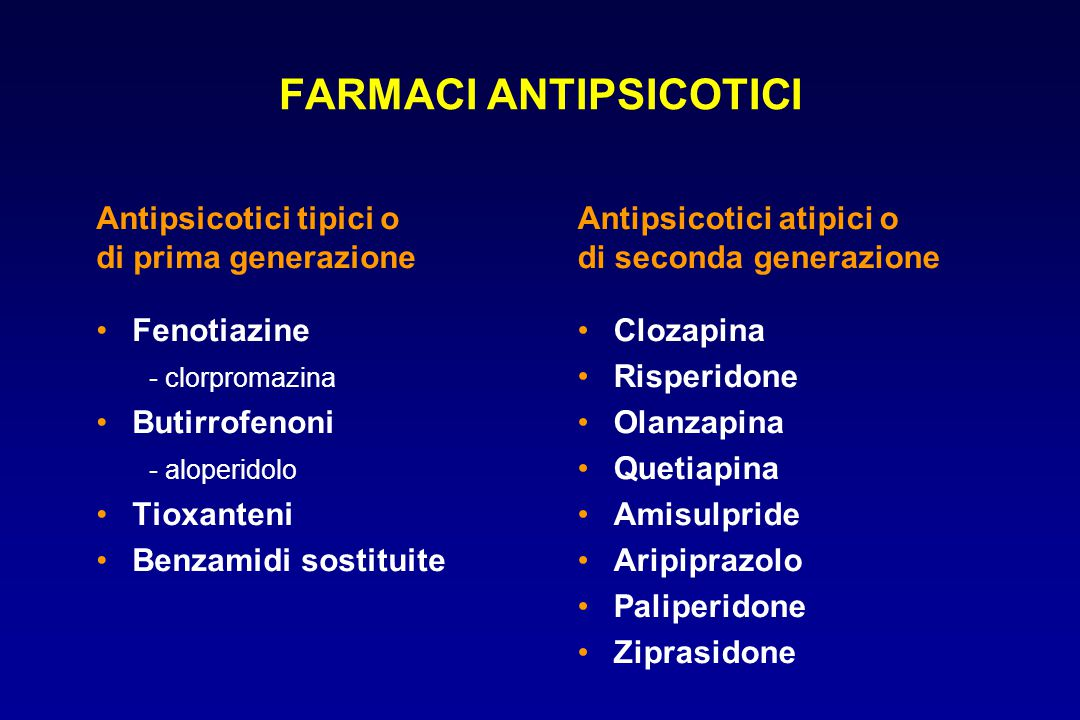
\includegraphics[width=1.92708in,height=2.98958in]{media/image1.jpeg}Dal
punto di vista della \textbf{farmacocinetica}, la \emph{velocità di
assorbimento} orale di questi sedativo-ipnotici dipende da diversi
fattori, in primis dalla loro \emph{liposolubilità}: ad esempio
l'assorbimento del triazolam è molto rapido, essendo questa una molecola
molto liposolubile così come lo è anche il diazepam e del clorazepam, e
la liposolubilità del composto è importante anche nello stabilire la
velocità con cui il farmaco supera la barriera emato-encefalica, andando
ad agire sui suoi bersagli recettoriali, ma è anche importante perché
consente al composto di \emph{superare la barriera emato-placentare},
infatti tutte le benzodiazepine sono controindicate in gravidanze,
poiché potrebbero dare gravi effetti sul feto e sul neonato, con
depressione delle funzioni vitali, e particolare attenzione va anche
posta al \emph{latte materno}, in cui le benzodiazepine si possono
accumulare. Per quanto riguarda il destino metabolico di questi farmaci,
essi vengono \emph{metabolizzati a livello epatico dal sistema del
citocromo P 450}, in particolare il \textbf{CYP3A4}, con processi di
ossidrilazione alifatica ed N-dealchilazione; i metaboliti
successivamente formati vengono quindi coniugati in reazioni di fase II
con l'acido glucuronico, ottenendo composti idrosolubili che vengono
quindi escreti tramite le urine. Tuttavia, molti metaboliti ottenuti
dalle reazioni di fase I sono ancora \emph{farmacologicamente attivi},
per cui l'effetto farmacologico può permanere più a lungo rispetto alla
semplice emivita farmacologica (quindi il loro uso dev'essere
attentamente controllato in caso di insufficienza epatica o epatopatie)
come nel caso del diazepam, che viene convertito in desmetildiazepam e
poi in oxazepam, il quale viene infine coniugato ed escreto con le
urine.

\emph{\emph{Effetti Farmacologici :}}

I principali effetti farmacologici legati alle benzodiazepine sono:

\begin{itemize}
\item
  \textbf{Sedazione ed Effetto Ipnotico};
\item
  \textbf{Effetto Ansiolitico};
\item
  \textbf{Effetto Anticonvulsivante};
\item
  \textbf{Effetto Miorilassante}, con riduzione del tono muscolare,
  sfruttato prevalentemente in ambito anestesiologico.
\end{itemize}

Se si volesse schematizzare, adottando un modello un po' artificioso,
gli effetti principali delle benzodiazepine possono essere così
suddivise:

\begin{itemize}
\item
  L'\emph{effetto ansiolitico} è maggiore con l'\textbf{alprazolam} ed
  il \textbf{lorazepam};
\item
  L'\emph{effetto ipno-inducente} è maggiore con l'\textbf{alprazolam} e
  il \textbf{triazolam};
\item
  L'\emph{effetto anti-convulsivante} è maggiore con \textbf{diazepam}.
\end{itemize}

\emph{\emph{Effetti Indesiderati}}

Un aspetto forse poco noto delle benzodiazepine sono le
\textbf{alterazioni a carico delle funzioni cognitive} causate dall'uso
di questi farmaci: nei pazienti, soprattutto se anziani, il trattamento
con benzodiazepine può dare \emph{alterazioni della capacità di
concentrazione}, un \emph{incremento dei tempi di reazione} ed anche
\emph{fenomeni anmesici}. Tutti questi effetti indesiderati non sono
unici del soggetto anziano, ma possono anche manifestarsi in soggetti
più giovani, anche se spesso in modo meno accentuato.

Le BDZ, in caso di sovraddosaggio, possono causare un \emph{sonno
prolungato} ma senza una depressione seria della funzione respiratoria o
cardiovascolare, tuttavia in pazienti con importanti patologie organiche
come le \textbf{BPCO} o in generale un'\textbf{insufficienza
respiratoria} potrebbero dare una \emph{grave depressione del centro del
respiro, con esiti potenzialmente anche letali}, e per tale motivo la
loro somministrazione è altamente controindicata in questo tipo di
pazienti, così come lo sono in pazienti a cui è stata diagnosticata una
concomitante \textbf{patologia neurologica}, poiché l'assunzione di
benzodiazepine potrebbe in questo caso determinare la comparsa di
\emph{atassia} ed \emph{ipotonia muscolare}.

Altri effetti collaterali meno frequenti sono poi le \emph{lipotimie} e
le \emph{disfunzioni sessuali}.

Dal punto di vista delle funzioni mentali, come già accennato le
benzodiazepine possono \emph{inficiare la memoria}, più nello specifico
interferiscono coi processi di consolidamento della \emph{memoria
verbale} (tipicamente il paziente riferisce di non riuscire a ricordare
i nomi delle cose o delle persone), e può essere interessata anche la
\emph{memoria a breve termine}, mentre quella a lungo termine è in
genere risparmiata. Si tratta generalmente di un'\textbf{\emph{amnesia
anterograda}}, cioè in questi pazienti si conserva la capacità di
ricordare nozioni o eventi del passato, ma non si riesce a fissare nuove
informazioni, e solo a dosi piuttosto elevate del farmaco può
effettivamente comparire un'amnesia totale, sebbene transitoria.

Da questi dati deriva ovviamente che le benzodiazepine
\emph{nell'anziano sono farmaci da usare con estrema cautela e solo se
necessario}, poiché in questo gruppo di pazienti i processi cognitivi
sono già di per sé compromessi e rallentati, e l'assunzione del farmaco
porterebbe inevitabilmente ad un peggioramento della situazione, dando
anche dei casi di \textbf{pseudo-demenza}. Sempre negli anziani,
inoltre, le benzodiazepine sembrerebbero in grado di suscitare una
particolare \emph{disinibizione comportamentale}, la quale è stata
descritta anche in soggetti affetti da disturbi della personalità, anche
se in quest'ultimo caso manchino ancora dei dati certi.

\emph{\emph{Meccanismo d'Azione:}}

Le benzodiazepine \emph{agiscono legandosi a specifici siti regolatori
allosterici posti a livello del recettore-canale}
\textbf{GABA\textsubscript{A}}, facilitandone l'apertura e
\emph{potenziando quindi l'effetto inibitorio del GABA stesso}. Si deve
tuttavia precisare che, a livello delle diverse aree cerebrali, esistono
diverse isoforme del canale GABA\textsubscript{A}, le quali differiscono
per l'affinità verso le benzodiazepine e quindi nella risposta al
farmaco stesso: le azioni di questi composti si esplicano pertanto in
prevalenza della \emph{corteccia frontale del sistema limbico}, mentre
l'azione anti-convulsivante si svolge a livello del \emph{tronco
encefalico}, gli effetti ipnotici sulla \emph{sostanza reticolare} e gli
effetti amnesici sempre sul \emph{lobo limbico}, in particolare
sull'\emph{ippocampo}.

\emph{\emph{Criteri di Scelta del Farmaco:}}

Uno dei criteri di scelta fondamentale che deve essere sempre preso in
considerazione nel momento in cui si valuta l'uso di una benzodiazepina
è l'\textbf{emivita} del composto stesso, che varia notevolmente da
farmaco a farmaco e consente di distinguere le benzodiazepine in:

\begin{itemize}
\item
  \textbf{\emph{BDZ a lunga emivita}}; come il \emph{diazepam} (Valium),
  che ha un'emivita di 20-100 ore (in alcuni casi arriva anche a 200
  ore!);
\item
  \textbf{\emph{BDZ ad emivita intermedia}}; come il \emph{clonazepam}
  (Rivotril), che ha un'emivita di 18-50 ore;
\item
  \textbf{\emph{BDZ ad emivita breve}}; quali il \emph{lorazepam}
  (Tavor, emivita di 11-20 ore), l'\emph{oxazepam} (Serax, Serenid,
  Serepax, emivita di 8-15 ore) e il \emph{lormetazepam} (Noctamid,
  emivita di 10-12 ore);
\item
  \textbf{\emph{BDZ ad emivita ultrabreve}}, come l'\emph{alprazolam}
  (Xanax, emivita di 6-12 ore) e il \emph{triazolam} (Halcion, emivita
  di 2-5 ore).
\end{itemize}

Le diverse emivite di questi composti dipendono essenzialmente dalla
loro \textbf{velocità di eliminazione}, infatti le benzodiazepine
differiscono notevolmente tra loro nella velocità con cui sono
metabolizzate a livello epatico e poi eliminate dall'organismo tramite
le urine: ad esempio l'emivita del triazolam (Halcion) è solo di 2-5
ore, mentre quella del diazepam (Valium) è molto maggiore, anche di 100
ore o più, e questo perché a livello epatico il diazepam viene
convertito in \emph{desmetildiazepam}, che conserva un'azione
farmacologica notevole, diversamente da quanto avviene col triazolam,
che non dà origine in maniera significativa a composti attivi dopo la
sua metabolizzazione. Chiaramente, se da un lato la lunga emivita
garantisce una copertura maggiore dei sintomi, dall'altro, a seguito di
un'assunzione giornaliera protratta, il farmaco \emph{può accumularsi
nei diversi tessuti}, in particolare nel \emph{tessuto adiposo}, per cui
la rimozione dell'effetto farmacologico avviene molto più lentamente.

Per questi motivi, in un soggetto depresso ma senza problematiche
particolarmente gravi è preferibile somministrare una BDZ a breve
emivita, che garantisca un buon effetto ipnotico alla sera ma che non
dia disturbi cognitivi al mattino seguente, come ad esempio il
lormetazepam (Minias), ma se il paziente ha un'insonnia di tipo
intermedio o terminale, con frequenti risvegli notturni, allora è bene
dare un farmaco ad emivita media, come l'alprazolam (Xanax), mentre le
benzodiazepine a lunga emivita, come il diazepam (Valium) sono oggi
molto meno usate che in passato, tanto che si preferisce non usarle
nemmeno in pazienti con funzionalità epatica integra, a meno che non sia
necessario un effetto terapeutico molto prolungato o, per motivi di
compliance, non sia possibile fare più somministrazioni giornaliere.

Se invece quello che si ricerca è un effetto prevalentemente
\emph{ansiolitico}, è bene ricorrere ad una benzodiazepina ad emivita
intermedia, come l'\textbf{alprazolam}, che viene dato prima a dosi
basse, aumentando poi la dose sino a portarla a regime, così da evitare
gli effetti collaterali connessi col suo utilizzo.

Recentemente, peraltro, sono stati introdotti in clinica anche alcuni
nuovi \emph{farmaci melatonino-simili}, come l'\textbf{agomelatina}
(Valdoxan/Thymanax), che ha una struttura simile a quella della
melatonina, ed agisce da agonista nei confronti dei recettori MT1 e MT2,
per cui possiede una blanda attività antidepressiva ed è anche utile per
regolarizzare il ciclo sonno-veglia, per cui se possibile si dovrebbe
cercare di sfruttare questi nuovi composti piuttosto che ricorrere con
eccessiva frequenza alle benzodiazepine.

\emph{\emph{Tolleranza e Dipendenza:}}

Uno dei principali problemi connessi con l'uso delle benzodiazepine è
che, se la loro somministrazione viene protratta nel tempo, si sviluppa
frequentemente un meccanismo di \textbf{tolleranza}, che è legata sia ad
un aumento del metabolismo dei farmaci a livello epatico, sia ad alcune
modificazioni recettoriali a livello delle membrane sinaitiche, tali da
richiedere un aumento progressivo delle dosi per raggiungere lo stesso
effetto che si otteneva prima con una dose minore. Strettamente
correlata col fenomeno della tolleranza è poi la \textbf{dipendenza}
dalla benzodiazepine, che è \emph{più comune in soggetti con disturbi
della personalità o in soggetti che hanno già una storia pregressa di
abuso d'alcol o sostanze}. Le benzodiazepine possono infatti dare sia
una \textbf{\emph{dipendenza fisica}} che una \textbf{\emph{dipendenza
psicologica}}: nella dipendenza psicologica tutte le attività svolte dal
soggetto diventano subordinate all'uso o all'acquisizione della sostanza
nei confronti della quale si ha la dipendenza, per cui il farmaco
diventa le preoccupazione principale della giornata del soggetto, mentre
nella dipendenza fisica compare una vera e propria sindrome da astinenza
legata alla mancata assunzione del farmaco, e in questi casi la
dipendenza da BDZ può creare non pochi problemi di diagnosi
differenziale, in quanto si manifesta con una sintomatologia in gran
parte sovrapponibile ai disturbi di panico.

Di fronte a questi problemi, nel caso in cui si ritenga opportuna la
sospensione del trattamento farmacologico è importante che il dosaggio
delle benzodiazepine sia \emph{ridotto in maniera graduale}, e
dev'esserci un impegno congiunto nell'affrontare degli incontri
medico-paziente più frequenti, ricordando al paziente il ruolo delle
benzodiazepine e le problematiche connesse alla loro assunzione prima di
intraprendere la terapia stessa.

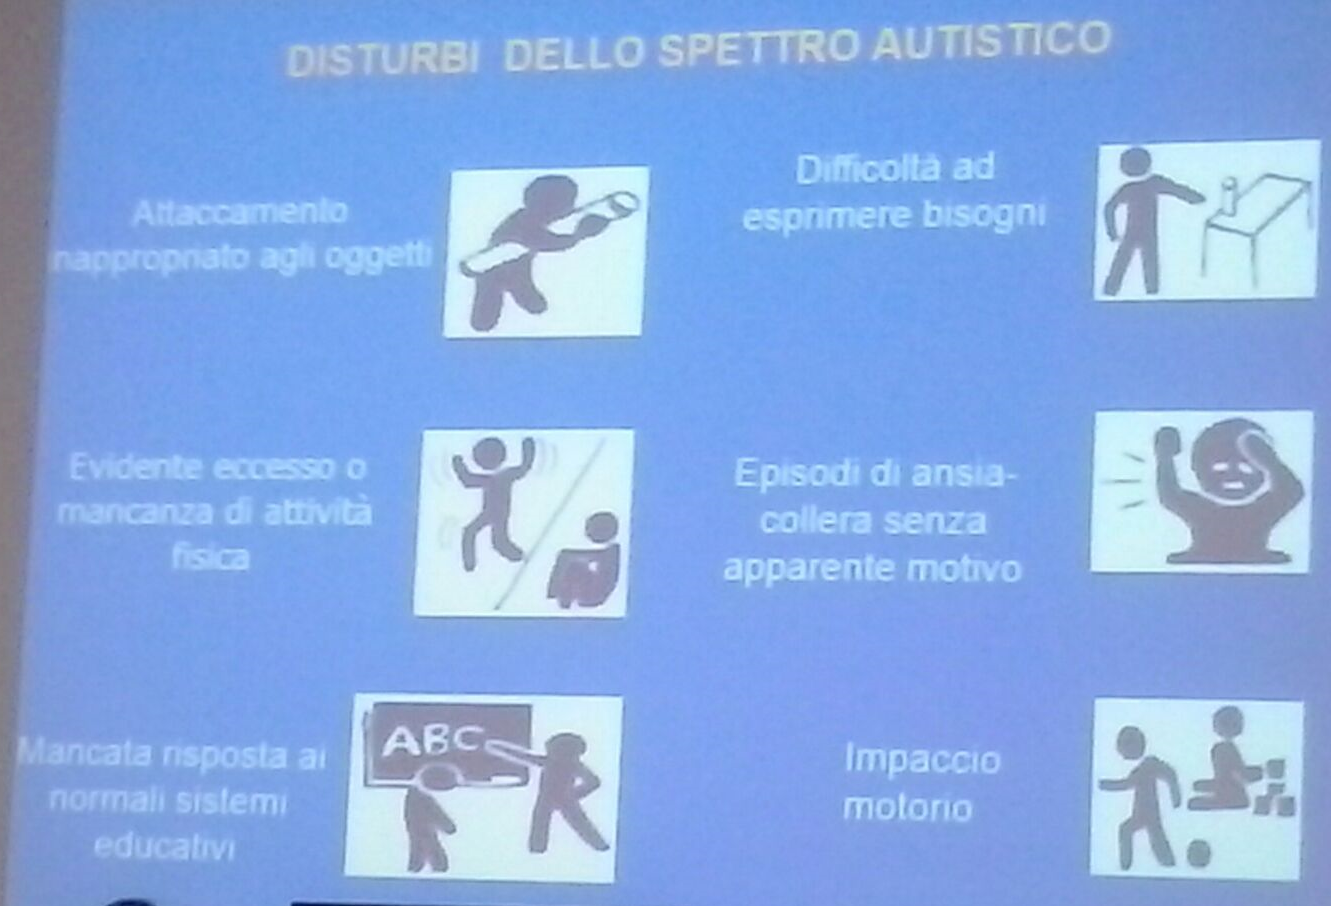
\includegraphics[width=2.40625in,height=1.85417in]{media/image2.gif}In
caso di \textbf{intossicazione}, infine, questa potrebbe risultare molto
seria in soggetti che hanno una pregressa patologia polmonare o
cardiocircolatoria di base, in quanto si potrebbe instaurare una
\emph{depressione del centro del respiro o di altri centri del tronco
encefalico}, e in questi casi è necessario intervenire con il
\textbf{\emph{flumazenil}}, un antagonista competitivo delle
benzodiazepine, che si lega al sito specifico di questi farmaci sul
recettore GABA\textsubscript{A} ma senza facilitarne l'apertura.

\begin{enumerate}
\def\labelenumi{\arabic{enumi}.}
\item
  \textbf{\emph{ANTIDEPRESSIVI:}}
\end{enumerate}

Gli ANTIDEPRESSIVI presentano il vantaggio di \emph{non causare
sedazione}, \emph{né assuefazione o dipendenza}, ma hanno il limite di
avere un \emph{periodo di latenza elevato} (occorrono almeno 2-3
settimane perché l'effetto farmacologico diventi chiaramente manifesto)
e paradossalmente possono causare dei \emph{sintomi panic-like} (perché
molti bloccano la ricaptazione della noradrenalina, per cui promuovono
un'attivazione del sistema nervoso simpatico), mentre le benzodiazepine
hanno il vantaggio di dare una \emph{rapida comparsa dei loro effetti},
ma d'altro canto \emph{causano sedazione, assuefazione e dipendenza}.

GlI \emph{\textbf{SSRI}} sono sempre da preferire ai TCA per i minori
effetti collaterali: questi farmaci hanno infatti \emph{minori effetti
anti-colinergici e cardiovascolari}, \emph{non provocano sedazione o
aumento ponderale}, sebbene possano comunque acere \emph{effetti sulla
sfera sessuale}, \emph{nausea, cefalea o insonnia}, così come gli
\emph{spiacevoli sintomi ``panic-like''} legati all'attivazione del
simpatico. A ciò va poi aggiunto che gli SSRI hanno una \emph{potenza
maggiore rispetto ai TCA}, per cui consentono al paziente di assumere un
numero minore di compresse, spesso permettendo anche una
mono-somministrazione giornaliera del farmaco. Gli SSRI attualmente in
commercio sono 6 (citalopram, escitalopram, paroxetina, sertralina,
fluoxamina e fluvoxetina) e sono tutti caratterizzati dall'agire tramite
un \textbf{blocco del trasportatore della serotonina} presente a livello
sinaptico, mentre differiscono leggermente tra loro per le ulteriori
azioni farmacologiche (vedi tabella).

\begin{longtable}[]{@{}lll@{}}
\toprule
\textbf{\emph{Farmaco}} & \textbf{\emph{Bersaglio d'Azione Primario}} &
\textbf{\emph{Altri Effetti}}\tabularnewline
\midrule
\endhead
\textbf{\emph{Escitalopram}} & SERT (Trasportatore della SERotonina) &
-\tabularnewline
\textbf{\emph{Citalopram}} & SERT & Blocco \textbf{recettori}
\textbf{H1}\tabularnewline
\textbf{\emph{Sertralina}} & SERT & Blocco \textbf{DAT}, interazione coi
\textbf{recettori σ} degli oppioidi\tabularnewline
\textbf{\emph{Fluvoxamina}} & SERT & Interagisce coi \textbf{CYP3A4} e
\textbf{CYP1A2}, interazione coi \textbf{recettori σ} degli
oppioidi\tabularnewline
\textbf{\emph{Fluoxetina}} & SERT & Blocco \textbf{NET}, Blocco
\textbf{recettori 5-HT\textsubscript{2}}, interagisce col
\textbf{CYP3A4} e \textbf{CYP2D6}\tabularnewline
\textbf{\emph{Paroxetina}} & SERT & Interagisce col \textbf{CYP2D6},
blocco dei \textbf{recettori M1}, blocco del \textbf{NET}, interagisce
con \textbf{NOS}\tabularnewline
\bottomrule
\end{longtable}

Visto che gli antidepressivi, sia gli SSRI che i TCA, necessitano di
\emph{almeno 2 settimane per dare i loro effetti}, \emph{in genere li si
associa alle benzodiazepine}, in modo da non lasciare ``scoperto'' il
paziente, poi l'ansiolitico può essere gradualmente tolto, in quanto gli
antidepressivi raggiungono il picco della loro azione in circa 8-12
settimane, e vanno mantenuti per almeno 6 mesi dopo la risposta
iniziale.

\begin{enumerate}
\def\labelenumi{\arabic{enumi}.}
\item
  \textbf{\emph{BETA BLOCCANTI:}}
\end{enumerate}

Altri farmaci spesso somministrati ai pazienti ansiosi sono i
\textbf{β-bloccanti} in monoterapia, i quali non si sono però dimostrati
efficaci nel ridurre la frequenza degli attacchi di panico o i sintomi
fobici, sebbene siano utili per il trattamento della sintomatologia
neurovegetativa.

\begin{enumerate}
\def\labelenumi{\arabic{enumi}.}
\item
  \textbf{\emph{PSICOTERAPIA COGNITIVO-COMPORTAMENTALE:}}
\end{enumerate}

Per quanto riguarda invece la \textbf{\emph{psicoterapia cognitivo-
comportamentale}}, essa prevede:

\begin{enumerate}
\def\labelenumi{\arabic{enumi}.}
\item
  una \emph{prima fase di psicoeducazione}, in cui si cerca di informare
  il paziente e di fargli comprendere la propria patologia,
\item
  poi si deve puntare sul \emph{monitoraggio costante dei sintomi in
  relazioni agli stimoli causali}, così da contrastare l'insorgenza
  dell'attacco di panico, e questo può essere ottenuto mediante
  l'apprendimento di specifiche \emph{tecniche di respirazione} ed una
  \emph{ristrutturazione cognitiva}, che consente al paziente di
  controllare il timore delle conseguenze dei sintomi, in modo da
  consentirgli di vincere l'ansia anticipatoria e riuscire così ad
  affrontare le situazioni temute.
\item
  \textbf{\emph{DECORSO:}}
\end{enumerate}

Per quanto riguarda il decorso del disturbo di panico, vari studi hanno
evidenziato che, dopo 4-6 anni dal trattamento, il 30\% dei pazienti si
trova in una condizione di benessere, il 40-50\% sta meglio ma conserva
un certo grado di sintomatologia, e solo il 20-30\% non mostra alcun
miglioramento o addirittura è peggiorato, mentre negli studi a lungo
periodo (20 anni), il 50\% dei pazienti si mantiene senza attacchi, il
30\% ha ancora sintomi, ma senza agorafobia o depressione, mentre il
10\%, pur essendo senza attacchi rilevanti, soffre di depressione o ha
comunque un certo grado di compromissione sociale. Tali dati sono molto
significativi, anche perché i pazienti con disturbo di panico tendono a
ricorrere al PS o all'intervento medico molto più frequentemente
rispetto alla popolazione generale, basti pensare che i pazienti ansiosi
sono responsabili del 6-12\% di tutte le visite ambulatoriali, si
rivolgono al PS circa 10 volte più spesso rispetto ai soggetti non
ansiosi e nel 70\% dei casi vengono valutati da almeno 10 medici prima
di giungere alla diagnosi corretta. Tipici sintomi somatici connessi col
disturbo di panico sono il \textbf{dolore toracico} e le
\textbf{palpitazioni}, per cui la diagnosi differenziale, che spesso
preoccupa notevolmente il paziente stesso, riguarda le patologie
cardio-vascolari: il dolore toracico dell'attacco di panico, tuttavia, è
un \emph{dolore atipico}, cioè \emph{non è retrosternale}, \emph{non è
legato a sforzo} e \emph{non passa col riposo o con la nitroglicerina},
come invece avviene nell'angina pectoris, per cui se il dolore è
atipico, il paziente è relativamente giovane, di sesso femminile, non ha
storia pregressa di coronaropatia ed ha anche elevati punteggi ai test
per l'ansia, la diagnosi di disturbo di panico è molto probabile, ed
anche le palpitazioni sono piuttosto comuni in questi paziente, tanto
che le cause psichiatriche sono al secondo posto, dopo quelle cardiache,
per lo sviluppo del cardiopalmo. Bisogna infine aggiungere, per
completezza, che alcuni studi avrebbero individuato una maggior
incidenza di \textbf{prolasso della valvola mitrale} in soggetto con
disturbo di panico, la il nesso causale tra queste due forme patologiche
non è stato ancora ben compreso.

\begin{itemize}
\item
  \textbf{\emph{DISTURBO OSSESSIVO-COMPULSIVO:}}
\end{itemize}

Caso clinico: \emph{ragazza 22-23 anni si reca a fare la babysitter e la
famiglia le affida un bambino di circa un anno e mezzo. Mentre sta
tenendo il bambino sente alla radio degli aggiornamenti sul caso del
delitto di Cogne: alla radio riferiscono che la madre era accusata di
aver ucciso il bambino in un raptus di follia. La ragazza ha il dubbio
di poter avere anche lei un raptus e lanciare giù dalla finestra il
bambino che le è stato affidato. Per la paura mette in atto tutta una
serie di provvedimenti atti ad impedirle di far male al bambino: abbassa
tutte le tapparelle, chiude il bambino a chiave in una stanza e nasconde
la chiave, prova a sentire il suo medico per sentire se fosse in grado
anche lei di fare come la Franzoni. Il medico, però, è a fare le visite
domiciliari e perciò la ragazza terrorizzata, in attesa di poter
ricontattare il medico si lega alla sedia con tutto ciò che riesce a
trovare; lascia libero solo un braccio in modo da poter usare il
telefono.}

\emph{Qual era il rischio per questo bambino di essere lanciato dalla
finestra?}

\emph{Esiste davvero il raptus?}

\emph{Il raptus non esiste, questo è dimostrato dal fatto che la
Franzoni non ha avuto un episodio di raptus (evolutosi in pochi
secondi), ma già ore prima aveva contattato la guardia medica in stato
ansioso dicendo che il suo bambino stava male.}

\emph{Questa situazione è molto diversa da quelle mamme estremamente
impulsive che perdono il controllo e sono talmente arrabbiate ed
esasperate che fanno del male al bambino. Non è un raptus, ma è
un'impulsività che non riesce più a essere frenata.}

\emph{La babysitter in realtà non era pericolosa, pur avendo un problema
di aggressività: l'idea di provare anche un minimo di rabbia è così
pericoloso da non poter nemmeno essere pensato, in quanto per questi
pazienti ciò che viene pensato automaticamente si realizza.}

Il DISTURBO OSSESSIVO COMPULSIVO è un disturbo di ansia che si
caratterizza per la \emph{presenza contemporanea di \textbf{ossessioni}
e di \textbf{compulsioni}}, che causano al paziente una notevole perdita
di tempo (in genere più di un'ora al giorno) o causano un
malfunzionamento sociale o occupazionale rilevante al paziente.

\begin{enumerate}
\def\labelenumi{\arabic{enumi}.}
\item
  \textbf{\emph{OSSESSIONI:}}
\end{enumerate}

Secondo i criteri del DSM, l'\textbf{ossessione} viene definita come:
una \emph{condizione caratterizzata dalla presenza di pensieri (}possono
essere di qualsiasi tipo, ma quelle che angosciano di più il paziente
sono quelle con risvolti aggressivi) \emph{o bisogni ricorrenti o
persistenti} che, ad un certo punto durante il disturbo, vengono
\emph{sperimentati dal paziente come intrusivi, indesiderati e/o
disturbanti}, tanto da causare \emph{ansia} o \emph{paura} nel paziente,
il quale \emph{tenta di sopprimerli o di ignorarli}, oppure cerca di
\emph{neutralizzarli ricorrendo ad altri pensieri o azioni}.

L'idea ossessiva, si distingue quindi dall'idea prevalente per il fatto
di essere \emph{egodistonica}, mentre l'altra è ego sintonica, \emph{non
ha rapporti diretti con l'affettività}, \emph{non viene accettata dal
paziente} (\textbf{fenomeno dello ``psichismo di difesa''}), viene
\emph{criticata come assurda} e \emph{limita l'espressione della
personalità} (al contrario l'idea prevalente può essere connessa ad
attività creative).

L'ossessione, inoltre, può essere facilmente distinta dal delirio per la
presenza della cosiddetta ``\textbf{meità}'', cioè ``\emph{l'io penso}''
Il paziente riferisce di fare l'azione in prima persona, quindi non è
posseduto da un'altra entità, nonostante l'azione non sia propria del
paziente.

Nei paziente deliranti la meità viene persa, poiché nel delirio si ha
certezza delle proprie credenze. Quindi è diverso dalle
\textbf{esperienze di passività} tipiche delle psicosi, dove tutto è
vissuto come se fossi un contenitore, un burattino e io facessi e
pensassi cose imposte da altri; si vive come posseduti da altri.

\emph{\emph{CASI CLINICI:}}

\begin{itemize}
\item
  \emph{Arriva una suora in ambulatorio che afferma di essere impazzita
  perché nella testa continua a bestemmiare. Cerca di fermarsi ma non
  riesce a bloccare questi pensieri. Questa situazione è diversa
  dall'esperienza di passività (esempio delirio di possessione
  demoniaca), perché il pensiero è riconosciuto come il proprio pur
  essendo egodistonico.}
\item
  \emph{Paziente si presenta in ambulatorio raccontando che gli si
  presentano nella mente delle immagini insistenti di presentatori TV
  che dicono porcate e che non riesce a eliminare. Le immagini sono
  proprie ma vissute come assurde rispetto al proprio carattere.}
\item
  \emph{Madre sente un fatto di cronaca dove una madre ha accoltellato i
  propri figli e le sorge il dubbio insistente di poter compiere lo
  stesso crimine. Per evitare di accoltellarli nasconde i coltelli e
  tutti gli oggetti appuntiti e, inoltre, fa un tentativo notturno
  entrando in camera dei figli con un coltello per vedere se provasse il
  desiderio di accoltellarli. Nonostante i vari tentativi si è convinta
  di poterlo fare e per questo motivo ha mandato i figli dalla madre e
  per poterli vedere bisognava che ci fosse presente qualcuno per
  controllarla.}
\item
  \emph{Uomo che si presenta dicendo che ha rovinato la famiglia perché
  è diventato omosessuale. Ciò è dovuto al fatto che ha sognato di
  andare in moto stretto ad un suo collega e nel sogno gli era piaciuto.
  Per verificare di essere realmente omosessuale aveva comprato riviste
  omosessuali, ma gli facevano schifo. Nonostante questo, non si era
  convinto e faceva anche delle prove entrando di soprassalto
  nell'ufficio del collega per verificare che non provasse sensazioni
  strane.}
\item
  \emph{Paziente si presenta in ambulatorio essendo convinto di aver
  contratto l'HIV dopo rapporti non protetti perché gli era venuto un
  mal di gola, nonostante le analisi del sangue fossero negative. Dopo
  un anno e mezzo richiama dicendo che gli è venuto il dubbio di potersi
  buttare giù dalla finestra e per questo motivo passa a circa due metri
  dalle finestre. Infine dopo circa due anni richiama richiedendo un
  certificato dove si afferma che non è omosessuale perché ha avuto
  delle prestazioni sessuali scadenti con la nuova morosa e qualche
  giorno prima i suoi amici l'hanno chiamato ``culattone'' e perciò gli
  è davvero venuto il dubbio di esserlo.}
\item
  \emph{Paziente si presenta in ambulatorio essendo convinta di avere la
  leucemia perché lavandosi i denti le erano sanguinate le gengive.
  Nonostante avesse fatto le analisi del sangue e queste fossero
  risultate negative, era convinta che fossero sbagliate e chiedeva ai
  medici se esisteva una leucemia con emocromo normale.}
\item
  \emph{Paziente si era convinta di ``fare la stupida'' con i passanti e
  che fosse rimasta incinta con questi ipotetici rapporti nonostante
  fosse in menopausa e l'ecografia fosse negativa.}
\item
  \emph{Paziente dopo aver ascoltato un programma televisivo in cui
  parlavano di melanoma e dei metodi per riconoscerlo, si era convinto
  di avere un melanoma in quanto presentava un nevo irregolare. Il
  paziente si era subito presentato in pronto soccorso la notte stessa
  per essere visto in urgenza ma, poiché i medici al triage gli avevano
  spiegato che la dermatologia non era aperta per questo tipo di
  patologie nelle ore notturne, si era arrabbiato temendo che in poche
  ore il tumore avrebbe potuto ucciderlo. }
\end{itemize}

\begin{enumerate}
\def\labelenumi{\arabic{enumi}.}
\item
  \textbf{\emph{COMPULSIONI:}}
\end{enumerate}

La \textbf{compulsione}, invece, viene definita come una
\emph{condizione che si caratterizza per la presenza di comportamenti o
atti mentali ripetitivi}, che il soggetto sente \emph{guidati dalla
necessità di rispondere ad un'ossessione} o ad una regola che dev'essere
applicata in maniera molto rigida.

Questi comportamenti o atti mentali sono finalizzati al \emph{prevenire
o al ridurre l'ansia e lo stress}, o per \emph{impedire qualche evento o
situazione temuta}, sebbene essi non siano in realtà connessi
realisticamente con ciò che il paziente suppone vadano a prevenire,
oppure sono chiaramente eccessivi.

Il soggetto li riconosce come eccessivi o irragionevoli, ma, nonostante
questo, non riesce a esimersi dall'eseguire queste azioni.

\emph{\emph{CASI CLINICI:}}

\begin{itemize}
\item
  \emph{Ragazzo si presenta in ambulatorio con il padre e sulla porta
  dello studio prima di entrare cammina avanti e indietro per circa 5
  minuti. Qualche giorno prima il ragazzo, litigando con un suo amico,
  gli aveva tirato un accidente e, per evitare che questo si avverasse
  davvero, si sentiva costretto a compiere questa azione un certo numero
  di volte.}
\item
  \emph{Paziente che, prima che tutta la famiglia potesse andare a
  letto, li faceva lavare con l'alcol: il marito, se non si lavava,
  doveva dormire sul divano. Inoltre era capitato che la madre al
  supermercato avesse incontrato un suo amico tossicodipendente e quindi
  la paziente l'aveva obbligata a buttare via la spesa appena fatta,
  perché credeva che fosse stata contaminata.}
\item
  \emph{Paziente che tutte le volte che esce nel cortile di casa deve
  farsi la doccia.}
\item
  \emph{Paziente che faceva il rappresentante di generi alimentari e a
  fine giornata doveva fare il riepilogo delle vendite davanti ai
  genitori più volte e se i genitori si rifiutavano si buttava a terra
  disperato.}
\item
  \emph{Paziente che aveva avuto dei contrasti con il comune e che per
  camminare sul suolo del comune aveva delle scarpe apposite che dopo
  buttava via. Una sera, a cena con la figlia, questa gli raccontò di
  essere stata in comune e lui allora, subito preoccupato, le chiese che
  scarpe aveva usato e gliele buttò nel camino.}
\item
  \emph{Paziente che mentre stava guidando sentiva un rumore provenire
  dalle ruote ed era convinto di avere investito qualcuno. Ad un
  incrocio aveva visto un ciclista passare e poi dopo non l'aveva più
  rivisto, finché il giorno dopo aveva letto sul giornale che un
  ciclista era stato investito. Si era convinto quindi che si trattasse
  proprio del ciclista che aveva visto e che fosse stato lui stesso ad
  investirlo. Era andato in ospedale a scusarsi con il ciclista, il
  quale ovviamente aveva smentito questa sua convinzione. }
\item
  \emph{Paziente dopo aver portato a scuola il figlio è stato preso da
  un incontrollabile bisogno di masturbarsi. Entra quindi nei bagni
  della scuola e si masturba, ma, arrivato a casa, si convince che ci
  fossero delle telecamere che l'hanno ripreso e che quindi era
  spacciato: le forze dell'ordine, vedendo il video, avrebbero
  certamente pensato che lui fosse un pedofilo e quindi sarebbero venuti
  ad arrestarlo. E anche se dopo qualche giorno non erano venuti ad
  arrestarlo, viveva nell'angoscia. }
\end{itemize}

Ovviamente, le ossessioni e le compulsioni non devono essere dovute
all'effetto fisiologico diretto di una sostanza o di una condizione
medica generale, ed il contenuto di queste manifestazioni non è
ristretto ai sintomi di altri disturbi mentali.

Il DSM, inoltre, raccomanda di specificare se il DOC è associato ad una
\textbf{buona capacità di insight}, cioè se il paziente si rende conto
che le sue credenze sono false o probabilmente false, o se vi è una
\textbf{scarsa} o \textbf{del tutto assente capacità di insight}.

Il DOC è quindi una patologia psichiatrica complessa, classificato tra i
disturbo d'ansia perché questa è la sua componente centrale, sebbene il
ruolo dell'ansia nella formazione dei sintomi è ben lontana dall'essere
chiarita. Caratteristica peculiare del DOC è la \textbf{\emph{fusione di
pensiero ed azione}}: i pazienti con DOC credono che pensare un evento
negativo lo possa far accadere, e che quindi pensare ad un evento
catastrofico equivalga eticamente a compierlo. Tipiche del DOC sono
anche varie \emph{alterazioni dell'attenzione e della vigilanza}, che
risultano aumentate per quelle parole che hanno un contenuto di
``contaminazione'', cioè ricordano maggiormente le parole a contenuto
negativo e vengono dimenticate più difficilmente. Frequente è anche
l'\emph{incapacità di inibire o spostare l'attenzione da pensieri o
azioni che creano disagio ad altri più piacevoli}, spesso assieme anche
ad alterazioni delle strategie organizzative e rallentamento
psicomotorio, che è conseguente al deficit delle strategie esecutive e
dell'attenzione e al dubbio sulle decisioni.

Il disturbo ossessivo-compulsivo ha una \emph{prevalenza life-time}
stimata del \textbf{2-3\%}, e presenta un'età media di esordio attorno
ai \emph{20 anni}, con una leggera predilezione per il \emph{sesso
femminile}.

All'interno del DOC si possono poi distinguere diversi sottotipi, come:

\begin{itemize}
\item
  il \textbf{DOC di contaminazione/lavaggio},
\item
  il \textbf{DOC di controllo},
\item
  quello di \textbf{collezione}
\item
  quello di \textbf{simmetria/ordine}.
\end{itemize}

Il decorso di questo disturbo è tendenzialmente cronico con fluttuazioni
di intensità dei sintomi, alcuni dei quali possono persistere anche dopo
un trattamento efficace, e spesso vi è un notevole intervallo di tempo
tra l'esordio dei sintomi e la diagnosi del DOC (in media 9 anni!).

L'eziopatogenesi del DOC non è stato ancora ben chiarito, tuttavia è
ormai ampiamente accettato che questo disturbo ha una \emph{base
genetica}, come dimostrato dal fatto che i familiari di primo grado di
un paziente con DOC hanno un rischio maggiore di sviluppare un disturbo
analogo, mentre tra gemelli omozigoti vi è un 67\% di concordanza,
rispetto al 31\% tra gemelli dizigoti, e vari studi hanno ipotizzato un
ruolo dei polimorfismi dei geni che codificano per il
\emph{trasportatore ed i recettori della serotonina}, nonché per i
\emph{recettori D4} della dopamina.

Altri studi hanno poi messo in luce diverse alterazioni
neuro-funzionali: nell'animale, infatti, l'attivazione della corteccia
pre-frontale e del nucleo caudato si associa a comportamenti ripetitivi
indotti da agonisti dopaminergici, mentre nell'uomo lesioni traumatiche
della corteccia orbito-frontale determina la comparsa del DOC, anche in
assenza di pregressi sintomi ossessivo-compulsivi, i quali possono
comparire anche in patologie in cui si ha una compromissione dei gangli
della base, come le PANDAS, e la terapia contro il DOC è in grado di
modificare positivamente l'attività pre-frontale e sottocorticale.

Queste evidenze hanno portato alla formulazione di \emph{due ipotesi
principali} per giustificare lo sviluppo del DOC, cioè l'\textbf{ipotesi
serotoninergica} e l'\textbf{ipotesi dopaminergica}: nella prima è
supportata dal miglioramento dei sintomi con la somministrazione di
SSRI, mentre la somministrazione di mCPP, un agonista serotoninergico
peggiora i sintomi; la seconda ipotesi si basa invece sull'osservazione
che l'amfetamina induce movimenti ripetitivi, mentre la cocaina accentua
i tic, e l'iperattività dopaminergica potrebbe essere secondaria alla
disfunzione del sistema serotoninergico.

\begin{itemize}
\item
  \textbf{\emph{DISTURBI DELLO SPETTRO OSSESSIVO:}}
\end{itemize}

Strettamente connessi col DOC sono i cosiddetti \textbf{\emph{Disturbi
dello Spettro Ossessivo}}, come la \emph{dismorfofobia},
l'\emph{ipocondria} e la \emph{sindrome di Tourette}, che spesso si
associano al DOC propriamente detto, ma non bisogna dimenticare anche il
\emph{disturbo del controllo degli impulsi} (cleptomania,
tricotillomania, gioco d'azzardo, autolesionismo e comportamenti
sessuali compulsivi), l'\emph{anoressia nervosa restrittiva} e le
\emph{coree di Sydenham e di Hungtington}.

Forma peculiari di DOC sono poi le \textbf{\emph{PANDAS}} (Pediatric
Autoimmune Neuropsychiatric Disorders Associated with Streptococcal
Infection), condizioni che si caratterizzano per la \emph{presenza di
sintomi ossessivi-compulsivi ed anomalie neurologiche}, come tic,
iperattività, movimenti coreiformi e deficit cognitivi. Possono poi
essere presenti anche labilità emotiva, ansia, irritabilità, incubi
notturni e comportamenti oppositivi. L'esordio delle PANDAS è in genere
in \emph{età pre-puberale} (in media attorno ai 6-7 anni), è
\emph{improvviso ed esplosivo}, con un decorso caratterizzato da
esacerbazioni e remissioni. La diagnosi è relativamente semplice, vista
le relazione temporale tra la comparsa dei sintomi, le esacerbazioni e
l'\textbf{infezione streptococcica}, che in genere precede l'esordio di
circa 6 settimane. Dal punto di vista della fisiopatologia, le PANDAS
sembrerebbero dovute appunto ad un'infezione streptococcica che si
sviluppa i pazienti con una certa suscettibilità genetica (in
particolare è stato molto studiato il ruolo dell'antigene D8/17 dei
linfociti B), per cui si viene a creare una \emph{risposta immunitaria
anomala con alterazioni infiammatorie a carico dei \textbf{gangli della
base}}, che danno appunto sintomi neuropsichiatrici. Il trattamento di
questi disturbi adolescenziali e prepuberali si avvale per prima cosa di
una \emph{terapia cognitivo-comportamentale}, e come trattamento di
seconda linea si ricorre alla somministrazione di \emph{antidepressivi
SSRI}, eventualmente associati alla CBT.

\begin{itemize}
\item
  \textbf{\emph{TERAPIA DEL DOC:}}
\end{itemize}

Per quanto riguarda la \textbf{\emph{terapia}} del disturbo ossessivo
compulsivo, anche in questo caso si hanno diverse opzioni terapeutiche,
quali:

\begin{enumerate}
\def\labelenumi{\arabic{enumi}.}
\item
  la somministrazione di \textbf{psicofarmaci} (in particolare
  \emph{SSRI})
\item
  la \textbf{psicoterapia} \textbf{cognitivo-comportamentale}
  (\textbf{CBT}),
\item
  diversamente dal disturbo di panico, nel DOC la risposta al placebo è
  scarsissima.
\end{enumerate}

In genere, nelle \emph{forme lievi/moderate} di DOC si ricorre prima
alla \emph{terapia cognitivo-comportamentale}, e solo come seconda linea
si può optare per l'uso di un \emph{SSRI}, eventualmente associato alla
CBT.

Nelle forme più \emph{severe} si parte direttamente con un \emph{SSRI} o
con l'\emph{associazione SSRI con CBT}.

\begin{enumerate}
\def\labelenumi{\arabic{enumi}.}
\item
  \textbf{\emph{PSICOFARMACI:}}
\end{enumerate}

\emph{\emph{Trattamento:}}

Nel trattamento farmacologico del DOC è fondamentale scegliere con
attenzione il farmaco e determinare la dose efficace, nonché la durata
appropriata del trattamento, inoltre bisogna valutare con cura il
trattamento dei pazienti pediatrici ed adolescenti.

Per quanto riguarda il primo punto, cioè la scelta del farmaco, diversi
studi hanno evidenziato che tutti gli \textbf{SSRI} e la
\textbf{cloripramina} (un TCA relativamente selettivo per il sistema
serotoninergico, è più potente rispetto agli SSRI, ma ha anche più
effetti indesiderati rispetto a questi) hanno un'efficacia superiore al
placebo, mentre gli altri antidepressivi non si sono dimostrati
superiore al placebo.

La dose standard del farmaco corrisponde in genere alla stessa dose
usata nella fase acuta, e le linee guida raccomandano di \emph{visitare
mensilmente il paziente per i primi 3-6 mesi} dall'inizio del
trattamento acuto, e di \emph{mantenere la terapia farmacologica per
almeno 1-2 anni}, che dev'essere tolta in maniera graduale e può essere
eventualmente da una terapia a lungo termine a scopo profilattico se si
verificano 2-4 riacutizzazioni severe oppure 3-4 riacutizzazioni lievi o
moderate.

Bisogna sempre fare attenzione alla sospensione della terapia del DOC,
perché non è infrequente riscontrare un peggioramento dei sintomi nelle
prime 4-8 settimane dalla sospensione degli SSRI, anche dopo un lungo
periodo di trattamento.

\emph{\emph{Risposta al trattamento:}}

Per quanto riguarda la risposta al trattamento, circa il 40-60\% dei
pazienti presenta un miglioramento medio dei sintomi dopo trattamento
con SSRI, ma \emph{raramente si arriva alla remissione completa}, pur
permettendo ai pazienti di lavorare, farsi una famiglia ed una vita
sociale attiva.

Sono \textbf{fattori prognostici negativi}, predittivi di una minor
risposta agli SSRI, una \emph{precoce età di esordio}, la \emph{presenza
di notevoli compulsioni}, la \emph{maggior gravità dei sintomi}, il
\emph{decorso cronico}, la presenza di \emph{ADHD} e di \emph{tics},
nonché l'\emph{associazione con disturbi di personalità} (DP
schizotipico).

In alcuni casi si può avere una resistenza al trattamento farmacologico,
che talvolta richiede però fino a 6 mesi per manifestarsi pienamente,
per cui le linee guida consigliano un cambiamento di farmaco dopo 8-12
settimane di non risposta o risposta parziale alla dose massima di un
SSRI, e in questi casi si ha una probabilità del 40\% di avere una
risposta ad un secondo SSRI. Se nonostante ciò si ha un fallimento con
2-3 SSRI, è bene passare alla psicoterapia.

\begin{itemize}
\item
  \textbf{\emph{FOBIA SOCIALE}}
\end{itemize}

È una disturbo d'ansia che si caratterizza per una \emph{paura marcata e
persistente di una o più situazioni sociali o prestazionali nelle quale
il paziente è esposto al giudizio degli altri} o comunque ad un contatto
con persone non familiari, per cui teme di agire (o anche solo di
mostrare sintomi d'ansia) in modo umiliante o imbarazzante.

L'esposizione alla situazione temuta quasi invariabilmente provoca
\emph{ansia}, che può assumere le caratteristiche di un attacco di
panico situazionale o sensibile alla situazione. Il paziente
\emph{riconosce che la sua paura è eccessiva o irragionevole}, e le
situazioni sociali o prestazionali temute sono evitate o sopportate con
intensa ansia o disagio, tanto che l'ansia anticipatoria e l'evitamento
delle situazioni sociali interferiscono significativamente col
funzionamento lavorativo o con le relazioni sociali del paziente.

Negli individui al di sotto dei 18 anni, per i criteri del DSM, la
durata dev'essere di almeno 6 mesi, e ovviamente questa condizione non
deve essere dovuta ad un altro disturbo mentale o ad una qualsiasi
condizione medica o fisica.

\begin{itemize}
\item
  \textbf{FOBIA SPECIFICA}
\end{itemize}

Secondo i criteri del DSM, la fobia specifica è un \emph{disturbo
d'ansia che si caratterizza per la presenza di paura marcata e
persistente, eccessiva ed irragionevole, provocata dalla presenza o
dall'attesa di un oggetto o situazione specifica} (ad esempio volare, le
altezze, gli animali, il ricevere un'iniezione, il vedere il sangue).
L'esposizione allo stimolo fobico quasi invariabilmente provoca una
\emph{risposta ansiosa immediata}, che si può presentare come un attacco
di panico situazionale o sensibile alla situazione, che nei bambini può
assumere forme peculiari, come il piangere, l'avere scoppi d'ira,
l'irrigidimento o anche con l'aggrapparsi a qualcuno. Il soggetto
riconosce che la sua paura è eccessiva ed irragionevole, ma non riesce a
farci niente, se non cercare di evitare al massimo la situazione temuta
o sopportarla con intensa ansia o disagio.

Come anche nel caso della fobia sociale, per i soggetti al di sotto dei
18 anni la sintomatologia deve persistere per almeno 6 mesi, e la fobia
deve determinare un deterioramento significativo del funzionamento
lavorativo o sociale del paziente, e non deve nemmeno essere dovuta ad
una condizione medica generale o ad un altro disturbo mentale.

\begin{itemize}
\item
  \textbf{DISTURBO D'ANSIA GENERALIZZATO (GAD)}
\end{itemize}

È un disturbo psichiatrico che si caratterizza per la \emph{presenza di
ansia e preoccupazione eccessiva}, che si manifestano \emph{per la
maggior parte dei giorni per almeno 6 mesi a riguardo di una notevole
quantità di eventi o attività}. Il soggetto ha difficoltà nel
controllare la preoccupazione, e l'ansia e la preoccupazione sono
associate ad almeno 3 dei 6 sintomi seguenti:

\begin{itemize}
\item
  \textbf{Irrequietezza}, \textbf{o} \textbf{sentirsi tesi o coi nervi a
  fior di pelle};
\item
  \textbf{Facile affaticabilità};
\item
  \textbf{Difficoltà a concentrarsi o vuoti di memoria};
\item
  \textbf{Irritabilità};
\item
  \textbf{Tensione muscolare};
\item
  \textbf{Alterazioni del sonno}.
\end{itemize}

L'ansia, la preoccupazione o i sintomi fisici causano un \emph{disagio
clinicamente significativo o una menomazione del funzionamento sociale,
lavorativo o di due aree importanti}.

\begin{itemize}
\item
  \textbf{DISTURBO POST-TRAUMATICO DA STRESS:}
\end{itemize}

È un disturbo in cui la persona è stata esposta ad un evento traumatico
in cui erano presenti entrambe le seguenti caratteristiche:

\begin{enumerate}
\def\labelenumi{\arabic{enumi}.}
\item
  \textbf{La persona ha vissuto, o ha assistito, ad un evento o a più
  eventi che hanno implicato la morte, o la minaccia di morte, o
  comunque al rischio di gravi lesioni rivolte all'integrità fisica
  propria o altrui}.
\item
  \textbf{La risposta della persona comprendeva un'intensa paura,
  sentimenti di impotenza o di orrore}.
\end{enumerate}

Nel disturbo post-traumatico da stress l'evento traumatico viene
rivissuto persistentemente in uno o più dei seguenti modi:

\begin{itemize}
\item
  \textbf{Tramite ricordi spiacevoli ricorrenti ed intrusivi
  dell'evento}, che comprendono immagini, pensieri o percezioni;
\item
  \textbf{Mediante sogni spiacevoli ricorrenti dell'evento};
\item
  \textbf{Tramite l'agire o il sentire come se l'evento traumatico si
  stesse ripresentando} (con flashbacks, illusioni, allucinazioni o
  altre forme);
\item
  \textbf{Intenso disagio psicologico o reattività fisiologica
  all'esposizione a fattori scatenanti interni o esterni} che
  simbolizzano o assomigliano a qualche aspetto dell'evento traumatico.
\end{itemize}

Ovviamente, a causa del disturbo, si ha un \emph{persistente evitamento
degli stimoli associati al trauma ed un attenuazione della reattività
generale}, come indicato da tre o più dei seguenti elementi:

\begin{itemize}
\item
  \textbf{Sforzi per evitare pensieri, sensazioni o conversazioni
  associate col trauma;}
\item
  \textbf{Sforzi per evitare attività, luoghi o persone che evocano
  ricordi del trauma;}
\item
  \textbf{Incapacità di ricordare qualche aspetto importante del
  trauma;}
\item
  \textbf{Riduzione marcata dell'interesse o della partecipazione ad
  attività significative;}
\item
  \textbf{Sentimenti di distacco o di estraneità verso gli altri;}
\item
  \textbf{Affettività ridotta;}
\item
  \textbf{Sentimenti di diminuzione delle prospettive future}.
\end{itemize}

Devono inoltre essere presenti \emph{sintomi persistenti di aumentato
arousal}, non presenti prima del trauma, come dimostrato dalla presenza
di almeno due dei seguenti sintomi:

\begin{itemize}
\item
  \textbf{Difficoltà ad addormentarsi o a mantenere il sonno;}
\item
  \textbf{Irritabilità o scoppi d'ira;}
\item
  \textbf{Difficoltà a concentrarsi;}
\item
  \textbf{Ipervigilanza;}
\item
  \textbf{Esagerate risposte di allarme}.
\end{itemize}

Infine, il disturbo deve \emph{durare più di un mese e deve causare un
disagio clinicamente significativo o una menomazione del funzionamento
sociale, lavorativo o di altre aree importanti}.

Il DSM suggerisce inoltre di specificare se di si tratta di una
\textbf{forma acuta} (la durata dei sintomi è inferiore ai 3 mesi),
\textbf{cronica} (la durata è di 3 mesi o più) o \textbf{ad esordio
ritardato} (se l'esordio dei sintomi avviene almeno 6 mesi dopo l'evento
stressante).

\end{document}

\documentclass[]{article}
\usepackage{lmodern}
\usepackage{amssymb,amsmath}
\usepackage{ifxetex,ifluatex}
\usepackage{fixltx2e} % provides \textsubscript
\ifnum 0\ifxetex 1\fi\ifluatex 1\fi=0 % if pdftex
  \usepackage[T1]{fontenc}
  \usepackage[utf8]{inputenc}
\else % if luatex or xelatex
  \ifxetex
    \usepackage{mathspec}
  \else
    \usepackage{fontspec}
  \fi
  \defaultfontfeatures{Ligatures=TeX,Scale=MatchLowercase}
\fi
% use upquote if available, for straight quotes in verbatim environments
\IfFileExists{upquote.sty}{\usepackage{upquote}}{}
% use microtype if available
\IfFileExists{microtype.sty}{%
\usepackage{microtype}
\UseMicrotypeSet[protrusion]{basicmath} % disable protrusion for tt fonts
}{}
\usepackage[unicode=true]{hyperref}
\hypersetup{
            pdfborder={0 0 0},
            breaklinks=true}
\urlstyle{same}  % don't use monospace font for urls
\IfFileExists{parskip.sty}{%
\usepackage{parskip}
}{% else
\setlength{\parindent}{0pt}
\setlength{\parskip}{6pt plus 2pt minus 1pt}
}
\setlength{\emergencystretch}{3em}  % prevent overfull lines
\providecommand{\tightlist}{%
  \setlength{\itemsep}{0pt}\setlength{\parskip}{0pt}}
\setcounter{secnumdepth}{0}
% Redefines (sub)paragraphs to behave more like sections
\ifx\paragraph\undefined\else
\let\oldparagraph\paragraph
\renewcommand{\paragraph}[1]{\oldparagraph{#1}\mbox{}}
\fi
\ifx\subparagraph\undefined\else
\let\oldsubparagraph\subparagraph
\renewcommand{\subparagraph}[1]{\oldsubparagraph{#1}\mbox{}}
\fi

% set default figure placement to htbp
\makeatletter
\def\fps@figure{htbp}
\makeatother


\date{}

\begin{document}

Classificazione delle Psicosi Endogene

\end{document}

\section{Schizofrenia}

\subsection{Storia}

\subsubsection{Kraepelin (1850)}

Primo concetto importante è che la schizofrenia non nasce con il nome di
schizofrenia, ma il primo nome che venne dato è di \textbf{Demenza
Precox} (significa letteralmente demenza precoce), cioè un quadro di
demenza, ovvero progressivo deterioramento della personalità, capace di
insorgere precocemente (età tra i 16 e 25 anni ) e dopo un decorso
progressivo portare ad uno stato di completa disgregazione.
\\\\
Il concetto di demenza precox nasce a cavallo tra `800 e `900 in un
periodo caratterizzato per la psichiatria di un completo nichilismo
terapeutico(non esistevano psicofarmaci). I primi farmaci per i disturbi
psichici nascono attorno anni '50, prima c'erano i manicomi e i medici
non potevano fare altro che osservare 24h su 24 senza la possibilità di
modificare il decorso della malattia. Anche la terapia elettroconvulsiva
(elettroshock) nasce nei primi del '900.
\\\\
Il termine demenza precox fu coniato da uno psichiatra tedesco di nome
\textbf{Emil Kraepelin} che è stato il fondatore della nosografia
psichiatrica, prima di lui erano già stati descritti segni e sintomi
psichiatrici, ma non era ancora stata data una coerenza nosografica.
\\\\
Kraepelin fece un'operazione semplice: divise i pazienti in due gruppi
secondo un criterio longitudiale, cioè secondo il decorso della malattia
e indipendentemente dai sintomi:

\begin{itemize}
\item
  \emph{Il primo gruppo era caratterizzato da un deterioramento
  progressivo} e quindi da un quadro cronico della patologia (non
  andavano in contro a remissione e stavano in manicomio tutta la vita);
\item
  \emph{il secondo gruppo era caratterizzato da quei pazienti che
  inspiegabilmente andavano incontro a remissione} anche dopo quadri
  gravi cronici.
\end{itemize}

Il primo modello classificatorio delle malattie mentali gravi era quindi
\textbf{in base alla prognosi}: quelli che guarivano e quelli che non
guarivano.

\begin{itemize}
\item
  Quelli che non guarivano erano inclusi nell'ambito della
  \textbf{demenza precox} (corrisponde alla moderna schizofrenia)
\item
  gli altri invece venivano classificati nell'ambito delle
  \textbf{psicosi maniaco depressive} (che corrisponde essenzialmente al
  disturbo bipolare, anche se autori successivi hanno poi distinto le
  forme di depressione unipolare)
\end{itemize}

Si notò che quelli che avevano una prognosi migliore erano quelli che
presentavano più frequentemente sintomi affettivi o in senso depressivo
o in senso espansivo; notò anche che i pazienti con psicosi
maniaco-depressive avevano un decorso fasico, ovvero episodico, con
episodi gravi e poi dopo risoluzione (a differenza del primo gruppo che
non aveva fasi, ma andava incontro a destrutturazione progressiva).
\\\\
Kraepelin incluse nella demenza precox quadri che erano già stati
precedentemente descritti come per esempio: la catatonia , ebefrenia,
visania atipica, tutte caratterizzate dall'esito infausto, dall'esordio
giovanile (in genere tra i 16 ed i 25 anni) e con un decorso più o meno
rapidamente progressivo che portava nell'arco di una decina d'anni ad
una condizione pressoché irreversibile.

Quindi riassumendo, il primo concetto importante è che Kraepelin fece
una distinzione e definì quella che poi venne definita schizofrenia in
base alla prognosi. L'unica possibilità di fare diagnosi, però, era il
tempo; il criterio di Krepelin era dunque un \emph{criterio
longitudinale}: non era possibile fare diagnosi al primo colloquio con
un paziente ma solo considerando l'evoluzione e il decorso clinico,
quindi la diagnosi di Dementia Precox veniva confermata quando si
riconosceva nel paziente l'evoluzione progressiva e l'esito infausto
(diagnosi a posteriori).

Quando parlava di demenza si riferiva ad uno stato degenerativo
difficile da immaginare, perché non c'erano farmaci e il decorso era
diverso da ora (epoca in cui ci sono i farmaci).

\subsubsection{Bleuler (1911)}

\begin{figure}[!ht]
\centering
	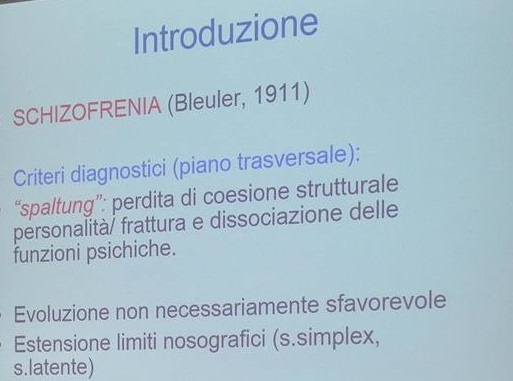
\includegraphics[width=0.9\textwidth]{06/image1.jpeg}
\end{figure}

\emph{\emph{Definizione:}}

Quindi il problema rimaneva di fare diagnosi: nel 1911 \textbf{Bleuler}
completò il concetto di \textbf{schizofrenia}, adottando non più un
criterio longitudinale, ma \emph{trasversale}: fare diagnosi a partire
dai sintomi.

Fu il primo a coniare il termine schizofrenia al posto di demenza
precox(che si rifà a concezione longitudinale invece che trasversale).
\\\\
Schizofrenina, letteralmente ``\textbf{\emph{rottura della mente}}'',
proprio per introdurre un \emph{criterio trasversale} e non più
longitudinale, ovvero indipendente dal decorso. Per Bleuler, la
schizofrenia è un disturbo che si caratterizza per una
\textbf{\emph{scissione}}, una ``\textbf{spaltung}'' \emph{delle
funzioni psichiche}, cioè una \emph{perdita della coesione strutturale
della personalità ed una dissociazione delle funzioni psichiche} che
porta, indipendentemente dal decorso, ad una \emph{discordanza}, ad una
\emph{frattura}, una \emph{disarmonia tra le varie funzioni psichiche},
in particolare l'\textbf{affettività}, la \textbf{memoria} e la
\textbf{coscienza}: ovvero tutto ciò che coinvolge la vita psichica
dell'individuo viene scissa, diventa discordante. Se riusciamo a
cogliere nel paziente questa perdita di coesione della personalità,
possiamo ipotizzare diagnosi di schizofrenia senza aspettare del tempo.

Le varie funzioni psichiche sono discordanti.
\\\\
\emph{\emph{Criteri:}}

Bleuler andò oltre e definì alcuni sintomi fondamentali per la diagnosi,
distinguendoli da quelli accessori (che potevano anche non esserci).
\\\\
\textbf{SINTOMI FONDAMENTALI:}

\begin{itemize}
\item
  disturbi affettività: apatia più o meno grave
\item
  abulia: perdita della volontà
\item
  autismo schizofrenico (non autismo infantile)
\item
  ambivalenza
\item
  dissociazione ideica
\end{itemize}

Sintomi tutti in negativo.
\\\\
\textbf{SINTOMI ACCESSORI:}
\begin{itemize}
\item disturbi percettivi
\item deliri
\item disturbi memoria e della personalità
\item sintomi catatonici
\end{itemize}

\begin{figure}[!ht]
\centering
	
\includegraphics[width=0.9\textwidth]{06/image2.jpeg}
\end{figure}

Distinse anche i sintomi in un altro modo (che non ha a nulla a che fare
con la distinzione precedente)
\\\\
\textbf{PRIMARI} = non generati da altri sintomi (disturbi associativi,
perturbazione umore di fondo)
\\\\
\textbf{SECONDARI} = conseguenza di sintomi primari (autismo,
ambivalenza, deterioramento schizofrenico, deliri, sintomi catatonici)

Ad es autismo schizofrenico è sia sintomo fondamentale ma anche
secondario (a deliri e allucinazioni)
\\\\
Caratteristicamente lo schizofrenico è identificato come una persona
soggetta ad allucinazioni, deliri, catatonia. I sintomi fondamentali,
ovvero l'essenza della schizofrenia, non sono questi sintomi eclatanti:
anzi questi appartengono a molti quadri clinici diversi anche dalla
schizofrenia. La schizofrenia non è questo quadro.
\\\\
Ad esempio:\emph{ragazzi che si chiudono in casa e a cui non importa più
di fare nulla, sono trascurati e l'eloquio comincia a disgregarsi
indipendentemente dai deliri e allucinazioni.}

Anzi i quadri più gravi sono quelli caratterizzati da questi sintomi
negativi.

\emph{\emph{Decorso:}}

I sistemi nosografici attuali ereditano i concetti storici. Importante
ricordare è che la \emph{schizofrenia ha un decorso cronico e non
fasico: una volta che inizia, tende ad avanzare.} Questo decorso cronico
porta sempre ad un meno rispetto a prima.
\\\\
La schizofrenia, inoltre, può instaurarsi sia come
\textbf{\emph{processo}} che come \textbf{\emph{sviluppo}}:

\begin{itemize}
\item
  \emph{Come processo}: esordio acuto o iperacuto. l'entità morbosa si
  abbatte improvvisamente e senza preavviso sul soggetto, spezzando la
  continuità di significato della vita di quel paziente
\end{itemize}

Il paziente era in un modo e nell'arco di pochi giorni o mesi inizia a
presentare sintomi che lo portano a distaccarsi da quello che era
precedentemente.

Sintomi di solito positivi: deliri, allucinazioni. Talvolta può avvenire
a più tappe: fase acuta, parziale remissione, altra fase acuta e
progressione (prognosi più favorevole).

\begin{itemize}
\item
  \emph{Come sviluppo}: non acuta ma subdola, graduale, meno eclatante.
\end{itemize}

Lento scivolamento a partire da tratti di personalità morbosi che erano
predisponenti alla malattia. Persone che da sempre erano introverse, con
difficoltà di relazione che, però, funzionavano: quindi personalità
predisposte, che nell'arco di mesi cominciano, ad esempio, a chiudersi
in casa o distaccarsi progressivamente. Di solito meno importanti
sintomi produttivi, ma sono in primo piano i sintomi negativi, con
completa destrutturazione personalità. Sono i casi più a rischio di non
essere individuati precocemente ( prognosi più sfavorevole). Più di
frequente essa esordisca a partire da una personalità premorbosa,
condizione nota come \textbf{schizoidia}, la quale non è quindi una
malattia, ma un tratto di personalità predisponente alla schizofrenia, e
la si ritrova:

-nel \emph{DP schizotipico}

-nel \emph{DP schizoide}

Nella schizoidia è presente una personalità con una tendenza al
disadattamento progressivo che favorisce quindi la nascita della
schizofrenia.
\\\\
La schizoidia si caratterizza per una peculiare disposizione e tendenza
a porre una distanza tra sé e l'ambiente, e la persona appare chiusa,
introversa, quasi fredda, non ricercando l'amicizia o il contatto con
gli altri; non sono timidi ma sono semplicemente disinteressati, poiché
presi da interessi personali inusuali, che non condividono con altri.
\\\\
Altra caratteristica della schizoidia è un'\textbf{anomala}
\textbf{proporzione psicoestesica}, ovvero la compresenza di
\emph{iperestesia} (elevata sensibilità e suscettibilità alle critiche)
e \emph{anestesia affettiva} (indifferenza alla rete delle relazioni
sociali).

\subsubsection{Schneider (1967)}

\begin{figure}[!ht]
\centering
	
\includegraphics[width=0.9\textwidth]{06/image3.jpeg}
\end{figure}

Il tedesco \textbf{Schneider} aggiunge un ultimo tassello. Da una parte
la schizofrenia è un processo neurodegenerativo che rimane soprattutto
caratterizzato da sintomi negativi, ma Schneider dice una terza cosa:
spesso è difficile riconoscere questi sintomi fondamentali, che sono più
fini dei sintomi negativi, con il rischio di ritardare la diagnosi.

Lui identifica dei sintomi positivi che sono caratteristici della
schizofrenia (come deliri e allucinazioni) che hanno la caratteristica
fondamentale di un vissuto di PASSIVITA'.
\\\\
Sono i \textbf{\emph{SINTOMI di PRIMO RANGO}}, altamente predittivi di
schizofrenia:

\begin{itemize}
\item
  \textbf{Allucinazioni uditive o pseudo allucinazioni: }
\end{itemize}

\begin{itemize}
\item[1.]
  possono essere VOCI TELEOLOGICHE: danno consigli e possono essere
  banali e far compagnia al paziente continuamente;
\item
  possono essere DIALOGANTI: dialogano tra loro, avendo come argomento
  il paziente, spesso ne parlano male
\item
  possono essere IMPERATIVE: danno ordini a volte banali, oppure
  addirittura di uccidersi o uccidere. Sono voci difficili da gestire,
  con pazienti che spesso non riescono a farle passare e quindi eseguono
  gli ordini che queste voci impongono, anche se non coincidono con la
  loro reale volontà. Quindi interferiscono molto con la vita del
  paziente;
\item
  possono essere voci COMMENTANTI gli atti del paziente;
\item
  possono essere come ECO DEL PENSIERO: ovvero ripetono quello che il
  paziente pensa e lui ha paura che gli altri possano sentirle.
\end{itemize}

\emph{Queste voci hanno in comune la perdita della barriera tra l'io
intimo e il mondo, c'è senso di permeabilità tra il paziente e il
mondo.}
\\\\
n.b: Sono presenti anche in disturbi depressivi e maniacali ma nella
Schizofrenia sono di tipi particolari e interferiscono con la vita del
pz.
\\\\
Altro sintomo di primo rango di Schneider:

\begin{itemize}
\item
  \textbf{Passività di pensiero}: paziente non più padrone del suo
  pensiero, imposto da altri.

\begin{itemize}
\item[1.]
  Paziente distaccato da propri pensieri, fino a quando non diventa più
  suo pensiero, ma è il pensiero di un altro inserito nella sua testa.
  Come se fosse costretto così a pensare il pensiero di un altro, questa
  è l'INSERZIONE DEL PENSIERO;
\item[2.]
  Oppure il FURTO DEL PENSIERO: il paziente pensa e il pensiero gli
  viene rubato da un altri. Questi vissuti espongono a deliri definiti
  DI SPIEGAZIONE dove il paziente cerca di darsi delle spiegazioni (ad
  esempio tramite sistemi satellitari, onde elettromagnetiche, ovvero
  spiegazioni deliranti);
\item[3.]
  Anche fenomeni di LETTURA del pensiero, il pensiero del paziente è
  letto da altri spesso tramite macchinari, attraverso cose fisiche;
\item[4.]
  DIFFUSIONE del pensiero: i pensieri dal paziente diffondono e si
  trasmettono agli altri.
\end{itemize}

Tutto ciò si manifesta quindi spesso sotto forma di deliri, altre volte
i sintomi di primo rango si manifestano sotto forma allucinatoria di
vario tipo (ad esempio allucinazioni visive di diffusione del pensiero).

\item
  \textbf{Passività somatica}: estraneità del proprio corpo (ad esempio
  altri che tramite mezzi ordinano o muovono parti del corpo senza
  volerlo). Il paziente riferisce di non essere lui a voler fare un
  movimento, ma è costretto, come una marionetta, e lo stesso vale anche
  per le altre funzioni biologiche, come la minzione.

Bisogna distinguere 2 momenti di gravità differente:

\begin{itemize}
\item
  perdita del senso di proprietà: ad esempio il braccio non è più il suo
  ma è stato sostituito (più grave)
\item
  perdita del senso di agenzia: ad esempio non è lui che muove braccio
  ma sono gli alieni ma il braccio è sempre del paziente.
\end{itemize}

Caso clinico: \emph{il prof fa l'esempio di un suo paziente che riferiva
non essere padrone della sua minzione perché la decisione di mingere gli
veniva imposta da un vecchietto appollaiato sulla sua prostata, quindi
passività somatica associata a delirio di interpretazione.}
\end{itemize}

Altri sintomi di primo rango secondo Schneider sono poi:

\begin{itemize}
\item
  \textbf{Passività di volontà e affettività}: volontà e sentimenti
  affettivi comandati o voluti da altri.
\item
  \textbf{Percezione delirante} (rara): poggia su un substrato di
  PASSIVITA' DI PERCEZIONE. La percezione delirante è una percezione
  corretta, ma a questa viene attribuita un significato abnorme ( caso
  clinico:\emph{paziente entra in una stanza vede una sedia e da lì
  capisce l'imminente venuta di Cristo sulla terra}). E' una passività
  di percezione perché il paziente è investito dal significato.
\end{itemize}

Diverse sono le interpretazioni deliranti (molto più frequente, non solo
nella schizofrenia ) che non sono sintomi di primo rango (caso clinico:
\emph{paziente vede semaforo rosso e dice che è rosso sangue e allora
significa che lo vogliono uccidere, il paziente attivamente attribuisce
significato al percetto)}. Nella percezione delirante non c'è questa
attività, ma è tutta passività, la modalità è rivelatoria, non di
conferma.

I sintomi di primo rango hanno una modalità molto fisica, il paziente
sente fisicamente le cose per esempio i pensieri di altri che entrano in
lui li sente entrare, come se bruciasse la pelle.

Abbiamo una spazializzazione del pensiero: li sentono fisicamente
(\emph{ad esempio pensieri che sentono dietro l'orecchio}). Questo si
manifesta non solo per la passività di pensiero ma per tutti i livelli
di passività, anche per la passività somatica (ad esempio:
\emph{paziente che sente omino che sta sulla sua prostata che gli dice
quando deve andare in bagno}).

In tedesco questi disturbi di passività si definiscono
\emph{``\textbf{\emph{gemacht}}= participio passato di fare'': il
pensiero è fatto da altri} e tutto è vissuto in termini spazializzati,
fisici.

C'è un altro termine che corrisponde al ``gemacht'', il corrispettivo
dell'ambiente: ``\emph{\textbf{\emph{gestelt}}} = collocato, messo lì''.
Si manifesta molto nelle fasi iniziali. Tutto quello che il paziente
vede è messo lì apposta, come se fosse tutta una trama di una
sceneggiatura, scritta apposta per il paziente (ad esempio:
\emph{qualcuno ha messo un telecomando qui apposta per me per dirmi
qualcosa}); tutto ruota attorno al paziente.

Per la diagnosi attualmente devono essere presenti più sintomi di primo
rango di Schneider ma ancora più importante del numero è la pervasività
dei sintomi, cioè la loro incidenza nella vita psichica del pz.


Poi abbiamo i \textbf{\emph{SINTOMI DI SECONDO RANGO}} : sebbene siano
importanti non consentono la diagnosi di schizofrenia, e sono
rappresentati da:

\begin{itemize}
\item
  \emph{intuizioni deliranti},
\item
  \emph{disturbi psico-sociali},
\item
  \emph{disturbi depressivo-euforici}
\item
  \emph{ottusità affettiva}.
\end{itemize}


Quindi \emph{riassumendo} la Schizofrenia è:

\begin{itemize}
\item
  per \textbf{Krepelin}, una condizione a \emph{evoluzione verso la
  demenza}, indipendentemente dai sintomi.
\item
  per \textbf{Breuler}, una condizione caratterizzata dalla
  \emph{frattura dello psichismo}, indipendentemente dal decorso.
\item
  per \textbf{Schneider}, una condizione caratterizzata dal
  \emph{vissuto di passività.}
\end{itemize}

\begin{figure}[!ht]
\centering
	
\includegraphics[width=0.9\textwidth]{06/image4.jpeg}
\end{figure}

\subsection{Manifestazioni cliniche della schizofrenia}

\subsubsection{Autismo schizofrenico}

\paragraph{Bleuler}

Inserito da Bleuler nel 1911 tra i sintomi fondamentali.

Definizione classica:

\begin{itemize}
\item
  \emph{distacco dalla realtà,}
\item
  \emph{interiorizzazione dell'affettività} (si intende che
  l'affettività è introiettata verso l'interno, verso le proprie
  fantasie e interessi strampalati e non verso l'esterno o verso gli
  altri.
\item
  \emph{prevalenza di un pensiero dereistico} (che non tiene conto della
  realtà).
\end{itemize}

Bleuler con autismo intendeva un sintomo fondamentale della
schizofrenia, ma secondario, non primario, che corrispondeva al
progressivo distacco dalla realtà: ovvero il paziente non è più
interessato alle cose del mondo, della realtà e si chiude nel suo mondo
delirante, fantastico. Questo distacco si evince da un pensiero
destrutturato, da una \emph{perdita del senso comune} (common sense)
quindi la perdita di ciò che per noi è pre-riflessivo (non ci dobbiamo
pensare) e che ci permette di vivere in mezzo agli altri, tanto che i
pazienti si comportano un po' come degli alieni, non sanno più come
parlare o interagire con gli altri e non riescono nemmeno a
comprenderli.

\paragraph{Minkowsi}

Il concetto di autismo fu approfondito poi da un altro autore, Eugène
\textbf{Minkowski} (1927), che lo fece diventare il cardine della
schizofrenia.

Definisce l'autismo schizorfrenico come una \textbf{\emph{condizione di
perdita del contatto vitale con la realtà o una perdita dell'evidenza
naturale}}, cioè il paziente perde quel qualcosa che normalmente non era
consapevole di possedere, ma che gli consentiva di mantenersi attaccato
alla realtà. Ovvero quello che il paziente perde è quel qualcosa a cui
noi non pensiamo perché è riflessivo: quel qualcosa che serve per
interagire con gli altri, per fare le cose che sappiamo dalla nascita e
che il paziente va a perdere nella schizofrenia.

Minkowski divide l'autismo in:

\begin{itemize}
\item
  AUTISMO RICCO: è quando questo distacco dalla realtà è accompagnato da
  una ricca produttività delirante, allucinatoria.

Ad es un pz chiuso nella sua stanza vive mondi fantasmagorici (esempio
di un pz che ogni giorno andava su Orione per accoppiarsi con una
principessa aliena)

\item
  AUTISMO POVERO: distacco accompagnato dal nulla, i pazienti stanno in
  casa senza fare nulla, guardano il soffitto (molto più grave della
  forma ricca).
\end{itemize}

Secondo Minkowski, questa condizione può essere presente anche nelle
\textbf{\emph{personalità pre-morbose}}, dove assume il nome di
\textbf{attività autistica} e comprende essenzialmente 3 forme:

\begin{itemize}
\item[1.]
  RAZIONALISMO MORBOSO: il significato comune delle cose viene perduto,
  il paziente cerca di ricodificare la realtà in modo
  iper-razionalistico (ad esempio: \emph{padre che regala alla figlia
  malata di tumore una bara}). C'è un completo distacco dall'evidenza
  naturale del normale vivere comune.
\item[2.]
  GEOMETRISMO PATOLOGICO: (ad esempio: \emph{paziente che, prima di
  esordire, diceva di non riuscire a capire il perché il sabato sera si
  dovesse uscire con gli amici; gli era talmente inspiegabile da
  convincersi che i suoi amici con la macchina descrivessero dei
  triangoli, di cui lui doveva calcolare l'area}). Senso geometrico
  della realtà.
\item[3.]
  REVERIE (fantasticherie morbose): i pazienti si chiudono nel loro
  mondo e non vivono. Si costruiscono una realtà di fantasticherie
  simili a quelle dei bambini, non sono dei deliri (ad esempio:
  \emph{una paziente, vissuta in casa tutta la vita in condizioni
  pessime, si era presentata alla visita, raccontando di essere la
  fidanzata di Lapo Elkann, di essere una modella. Il tutto con la
  consapevolezza di non aver davvero compiuto i fatti dei suoi racconti,
  era solo una fantasia}).
\end{itemize}

\paragraph{Biswanger}

Dopo Minkowski un altro autore (\textbf{Biswanger}) definì altre 3
caratteristiche dell'autismo schizofrenico, \textbf{le 3 forme
dell'esistenza mancata:}

\begin{figure}[!ht]
\centering
	
\includegraphics[width=0.9\textwidth]{06/image5.jpeg}
\end{figure}

\begin{itemize}
\item[1.]
  ESALTAZIONE FISSATA: pazienti in cui la perdita di contatto con la
  realtà si manifesta perché si fissano su una cosa che fa capire quanto
  il paziente sia distaccato. ( ad esempio: \emph{paziente che si era
  fissato sull'amicizia per un suo amico, viveva per questa amicizia,
  non sono deliri}; oppu oppure ad esempio: \emph{paziente che viveva
  solo per capire il meccanismo dell'orgasmo femminile, si documentava
  tantissimo e scriveva e lo spiegava in modo schizofrenico,
  meccanicistico}).
\item[2.]
  STRAMBERIA: caratteristica dell' andare di traverso rispetto a quello
  che il senso comune (ad esempio: \emph{il paziente che regala la bara
  alla figlia}; oppure: \emph{andare in giro con il piumino ad agosto};
  \emph{paziente che dorme durante la messa}).
\item[3.]
  MANIERISMO (molto frequente nella schizofrenia): paziente imita in
  modo goffo come ci si dovrebbe comportare con gli altri (ad
  esempio\emph{: paziente che, quando vedeva il dottore, lo salutava in
  modo esagerato ogni volta, anche a distanza di pochi minuti}). Alcune
  forme di schizofrenia si caratterizzano primariamente con questo
  comportamento.
\end{itemize}

\subsubsection{Dimensioni della schizofrenia}

Attualmente, nei moderni sistemi nosografici, la schizofrenia viene
considerata come una sindrome che si caratterizza per la presenza di 3
dimensioni sintomatologiche:

\begin{itemize}
\item[1.]
  \textbf{\emph{DIMENSIONE NEGATIVA:}}

I sintomi negativi coincido con i sintomi fondamentali di
\emph{Bleuler}, ad esclusione dei disturbi di associazione delle idee
che rientrano nella dimensione di disorganizzazione.

I sintomi negativi sono l'elemento nucleare della schizofrenia perché
tendono a persistere, sono refrattari alla terapia farmacologica; sono
la dimensione che maggiormente impatta sull'esito, sul funzionamento
globale del soggetto. comprende le cosiddette ``\emph{4 A di Bleuler}'',
ovvero \textbf{apatia} 8mancanza di sensazioni), \textbf{abulia}
(mancanza di volontà), \textbf{anedonia} (mancanza di piacere) e
\textbf{alogia} (povertà di pensiero), da cui deriva il \textbf{ritiro
sociale}.

Diversamente dei sintomi positivi, quelli negativi, così chiamati
proprio per indicare la mancanza di capacità di interazione sociale,
\emph{non rispondono alla terapia farmacologica e tendono a permanere
nel tempo}.

I sintomi negativi si distinguono in \textbf{due gruppi}: primari e
secondari.

\begin{itemize}
\item
  I \textbf{sintomi secondari} sono secondari ad altro: secondari a
  terapie con farmaci neurolettici di prima generazione, secondari
  all'istituzionalizzazione (processo cronico di sottostimolazione
  ambientale) oppure secondari a sintomi positivi, ad esempio: un
  paziente delira, è convinto che ci sia un complotto contro di lui, che
  qualcuno stia cercando di ammazzarlo, di conseguenza si chiude in
  casa. I sintomi secondari possono essere corretti correggendo la causa
  che sta alla base.
\item
  I \textbf{sintomi primari}, che sono i più interessanti, tendono ad
  essere acquistabili nel tempo e sono refrattari alla terapia.
\end{itemize}

\emph{Caso clinico}: \emph{A tale proposito si riporta l'esempio di un
paziente (35 anni) affetto da schizofrenia il cui quadro è
caratterizzato prevalentemente da sintomi negativi, quadro grave: il
paziente a gennaio riceve un invito a pranzo dalla sorella (unica
persona con cui il paziente intrattiene relazioni sociali, una persona
molto accudente, carina, persona di fiducia) per Ferragosto (da notare
gennaio-agosto intercorrono sei mesi tra l'invito e il pranzo). Il
paziente è molto angosciato per l'invito nonostante il pranzo sia da lì
a sei mesi. Errore da psichiatra inesperto: insistere per convincere il
paziente a partecipare al pranzo perché ``siamo a gennaio, il pranzo è
ad agosto, hai sei mesi per fartene una ragione e andare'' perché questo
ragionamento non tiene conto del fatto che il paziente è abulico, è un
ragionamento da persona normale. Il paziente risponde ``dottore, lei ha
ragione ma la vita è per i sani'', tale espressione denota come per il
soggetto abulico (affetto da abulia, mancanza di volontà) tale pranzo
costituisca un ostacolo insormontabile. Quindi si comprende come i
progetti riabilitativi debbano tenere conto delle capacità e delle
risorse dei pazienti e non si debbano basare su un modo di ragionare da
persona sana. Richiedere al paziente abulico dell'esempio di partecipare
al pranzo dalla sorella equivale a richiedere che un paziente affetto da
morbo di Parkinson o con un femore fratturato di correre i 100 m: è
evidente che il paziente non è in grado; discorso analogo è valido per
il paziente abulico ma è più difficile rendersene conto perché l'abulia
è un sintomo che non si vede. }


\item[2.]
  \textbf{\emph{DIMENSIONE POSITIVA:}}

I sintomi positivi sono \textbf{deliri} e \textbf{allucinazioni}.

Sono detti positivi perché c'è qualcosa in più che non dovrebbe esserci.
I sintomi della dimensione positiva sono quelli che rispondono meglio
alla terapia farmacologica, potendo in alcuni casi attenuarsi
spontaneamente.

(\emph{Nota bene: il delirio verrà trattato in una lezione apposita, qui
si tratterà di allucinazioni}).

\begin{itemize}
\item
  Le \textbf{\emph{ALLUCINAZIONI PROPRIAMENTE}} dette sono percezioni
  senza oggetto, poste nel campo esterno. (ad es vedo un gatto che in
  realtà non c'è).


I pazienti affetti da schizofrenia possono soffrire di tutti i tipi di
allucinazioni propriamente dette (p.d.). I tipi più frequenti sono le
allucinazioni:


\begin{itemize}
\item[1.]
  \textbf{UDITIVE}: in assoluto più frequenti nella schizofrenia.
  Esempio di allucinazione uditiva: il paziente sente una voce provenire
  dalla strada (percezione senza oggetto perché la voce non esiste,
  posta nel campo esterno ovvero la strada).
\item[2.]
  \textbf{OLFATTIVE}: più frequenti nei disturbi affettivi e nelle
  depressioni psicotiche.
\item[3.]
  \textbf{VISIVE}: sono più frequenti negli stati organici come demenza,
  traumatismi, neoplasie. Esempio di allucinazione visiva: il paziente
  vede un gatto sulla scrivania ma sulla scrivania non esiste alcun
  gatto (percezione senza oggetto perché il gatto non esiste, posta nel
  campo esterno ovvero sulla scrivania).
\item[4.]
  \textbf{GUSTATIVE}
\item[5.]
  \textbf{CINESTESICHE}: I pazienti schizofrenici soffrono anche di
  allucinazioni cenestesiche, si tratta di allucinazioni che riguardano
  il proprio corpo.

\emph{Caso clinico: esperienza allucinatoria che un animale si muova
dentro il proprio corpo o che un organo si dislochi da un'altra parte.
Si tratta di sintomi di primo rango di Schneider che sottendono un
vissuto di passività.}
\\\\
\emph{Caso clinico}:\emph{Si riporta l'esempio di un paziente che
riferisce di sentire (attenzione: il paziente sente fisicamente, le
allucinazioni nella schizofrenia sono fisiche, concrete) ``l'ormone
della tiroide incastrato nel dotto che collega il cervello alla
tiroide'' e tenta di disincastrarlo con il dito ma purtroppo resta
incastrato causando un'atrofia di tutti i suoi caratteri e organi
sessuali motivo per cui il paziente sostiene di star diventando donna.
Si tratta di un'esperienza allucinatoria di tipo somatico che regge in
realtà un delirio di trasformazione ma alla cui base vi è il vissuto di
passività somatica. }
\\\\
Alle allucinazioni cenestesiche appartengono le allucinazioni
CINESTESICHE (si legge kinestesiche): l'allucinazione cinestesica è
l'esperienza allucinatoria che il proprio corpo si stia muovendo mentre
in realtà è fermo oppure che stia fermo mentre in realtà si sta
muovendo; dipende sempre da vissuti di passività somatica.

\item[6.]
  \textbf{APTICHE}: altre allucinazioni sono quelle aptiche: sensazioni
  di scossa elettrica forti e lunghe. \emph{Caso clinico}: Si riporta
  l'esempio di un paziente che ogni due minuti si alza dalla sedia come
  se fosse sulla sedia elettrica perché percosso da una scossa
  elettrica; si tratta di un'allucinazione aptica che sostiene deliri
  persecutori: il paziente è convinto che sia il vicino di casa ad
  indurre la scossa. Ancora allucinazioni tattili: i pazienti si sentono
  toccati e allucinazioni termiche: vengono vissute come folate di vento
  caldo o freddo che investe parti del corpo.
\end{itemize}

\item
  Le \textbf{\emph{PSEUDOALLUCINAZIONI}} sono percezioni senza oggetto,
  poste nel campo interno, forse ancora più frequenti delle
  allucinazioni che a differenza delle propriamente dette provengono non
  dal campo esterno ma dal campo interno.

\emph{Caso Clinico}: \emph{Esempio di pseudo allucinazione uditiva: il
paziente sente una voce provenire da dentro si sé, il paziente non è in
grado di capire che si tratta di una pseudo allucinazione ma
classicamente riferisce che sente delle voci perché gli è stato
impiantato un micro chip nella testa}

\item
  Le \textbf{\emph{ILLUSIONI}} (che non sono esclusive della
  schizofrenia ma si osservano anche nei disturbi affettivi) sono
  percezioni in cui l'oggetto esiste ma è percepito come deformato,
  talvolta in maniera orribile che spaventa il paziente. (ad esempio
  vedono il volto di una persona ma viene distorta la percezione e ad
  esempio il pz vede il volto andare in decomposizione).

\emph{Caso clinico}: \emph{Si riporta l'esempio di un paziente che
durante il giro visite ha sferzato un pugno al primario perché in preda
ad un'illusione, il paziente vede il volto del primario (l'oggetto
esiste) deformato in modo raccapricciante, come se si stesse
liquefacendo, come se fosse uno zombie, si spaventa e aggredisce il
primario. }

\item
  Le \textbf{\emph{ALLUCINOSI}} sono percezioni senza oggetto poste
  nell'ambiente esterno di cui il paziente è consapevole (il paziente ne
  riconosce il carattere morboso cioè sa che quello che vede in realtà
  non c'è) Questa è l'accezione del termine allucinosi nel contesto
  della schizofrenia, altrimenti per allucinosi si può intendere una
  sindrome allucinatoria come la sindrome allucinatoria alcolica.

Generalmente le allucinosi sono molto complesse, sceniche, di massa, ci
sono tante figure che fanno tante cose complesse e generalmente ma non
sempre sono indice di un quadro organico come la demenza.
\end{itemize}

\item[3.]
  \textbf{\emph{DIMENSIONE DISORGANIZZATIVA:}}

La dimensione disorganizzativa si distingue in ideativa, affettiva,
comportamentale.

La \textbf{\emph{DISORGANIZZAZIONE IDEATIVA:}} significa che il pensiero
è scucito cioè vengono persi i nessi logici tra le idee, il soggetto
attinge a nessi paralogici.

\begin{itemize}
\item
  Un esempio classico di disorganizzazione del pensiero è la
  \emph{SIMMETRIA PATOLOGICA}: il soggetto non è in grado di utilizzare
  in modo opportuno la simmetria. Esempio di uso opportuno della
  simmetria: \emph{``Marco è mio fratello, io sono fratello di Marco}''.
  Esempio di simmetria patologica: ``\emph{Marco è mio figlio, io sono
  figlio di Marco}''.
\item
  Un altro caratteristico disturbo del pensiero è il \emph{PRINCIPIO DI
  VON DOMARUS} in cui l'enunciato viene costruito in base all'identità
  dei predicati e non dei soggetti. Esempio: ``\emph{Io sono vergine, la
  Madonna è vergine, io sono la Madonna''. }
\item
  In generale si parla di \emph{PENSIERO DEREISTICO} quando il pensiero
  devia dalla realtà cioè non si attiene alle norme logiche della
  realtà.
\item
  Un altro disturbo formale del pensiero (caratteristico della
  schizofrenia ma non esclusivo, si osserva anche in alcuni disturbi
  dello spettro autistico) è la \emph{CONCRETIZZAZIONE DEL PENSIERO} che
  consiste nell'incapacità da parte del paziente di astrarre il
  significato non letterale, il paziente non è pertanto in grado di
  capire metafore e proverbi, non è in grado di andare al di la del
  significato letterale della frase.

\emph{Caso clinico}: \emph{Esempio classico: alla domanda ``come sta?''
il paziente schizofrenico risponde ``seduto''. Si riporta anche
l'esempio di un paziente che invitato a rimanere con ``i piedi per
terra'' si presenta con le scarpe in mano; si riporta l'esempio di un
paziente che si lascia convincere a partecipare ad escursione in
montagna perché ``potrebbe vedersi il mare'' inteso potrebbe vedersi il
Golfo di Spezia e si presenta in costume da bagno. }

\item
  Le forme estreme di incoerenza sono definite \emph{SCHIZOFASIA}, sono
  forme in cui viene perso completamente ogni nesso logico, la
  destrutturazione del pensiero è completa.
\end{itemize}

La \textbf{\emph{DISORGANIZZAZIONE COMPORTAMENTALE E DELLA VOLONTA'}}:
si può manifestare con:

\begin{itemize}
\item
  La \emph{CATATONIA} è peculiare di una particolare forma
  schizofrenica, la schizofrenia catatonica, e contrariamente a quanto
  si credeva in passato, non è un sintomo esclusivo della schizofrenia
  ma può essere presente anche in altri quadri clinici esempio la
  depressione, esiste infatti la depressione catatonica. Errore comune
  anche in ambito specialistico è confondere la catatonia con lo stupor
  cioè immobilità. Catatonia e stupor sono ben diverse. Nello stupor
  (sia che il paziente sia schizofrenico sia che sia depresso) il
  paziente è immobile. Anche nella catatonia il paziente è immobile ma è
  un'immobilità peculiare caratterizzata da due segni semeiologici che
  sono la flexibilitas cereas e la catalessia. Risponde bene alla
  terapia farmacologica.

\item
  FLEXIBILITAS CEREAS è un segno per cui cercando di mobilizzare l'arto
  del paziente si incontra una certa resistenza come se fosse un tubo di
  piombo o di cera. La resistenza è determinata dalla contrazione dei
  muscoli antagonisti al movimento; invece nello stupor, a differenza
  della catatonia, il paziente si lascia mobilizzare in modo normale.
\item
  CATALESSIA è il fatto che il paziente mantenga posizioni (anche
  scomode) che vengono fatte assumere passivamente dall'interlocutore.
  \emph{Caso clinico}: un paziente è catatonico e sollevo un braccio,
  questo tenderà a rimanere sollevato mentre nello stupor un braccio
  sollevato cade.
\end{itemize}

La manovra per la Diagnosi Differenziale tra catatonia e stupor al letto
del paziente consiste nel sollevare le gambe, se queste rimangono su
allora il soggetto è catatonico altrimenti è in stato di stupor.

È importante distinguere la catatonia dallo stupor perché la catatonia è
potenzialmente mortale.

Nella \emph{\emph{catatonia acuta grave di Stauder}} la mortalità
raggiunge il 15\%. Ciò è dovuto al fatto che nella catatonia i muscoli
sono contratti, nei casi gravi la catatonia questo comporta danno ai
muscoli con picco delle CPK, con possibile danno alle fibre muscolari
(rabdomiolisi) e morte per insufficienza renale.

La schizofrenia catatonica è diventata rara perché la catatonia risponde
bene e subito alla terapia farmacologica per cui è una forma che si vede
nei pazienti non trattati.

In passato schizofrenia catatonica era caratterizzata dall'alternanza di
fasi di:

\begin{itemize}
\item[1.]
  CATATONIA STUPOROSA (immobilità) e di brevi fasi di:
\item[2.]
  CATATONIA ECCITATA in cui improvvisamente i pazienti escono dal loro
  immobilismo ed entrano in uno stato di grave agitazione psicomotoria
  con comportamenti aggressivi pantoclastici (distruttivi) per poi
  ripiombare per mesi in uno stato di catatonia stuporosa.
\end{itemize}

Solitamente i pazienti affetti da schizofrenia catatonica possono avere
altri segni:

\begin{itemize}
\item
  STEREOTIPIE VERBALI o MOTORIE cioè ripetizione di parole senza senso o
  ripetizione di atti;
\item
  NEGATIVISMO che può essere attivo o passivo. Negativismo passivo in
  cui il paziente non risponde ai comandi, ordini, consigli; negativismo
  attivo (un tempo si vedeva molto più frequentemente) in cui il
  paziente esce dal suo immobilismo ma risponde in modo assolutamente
  contrario a quanto viene chiesto.
\end{itemize}

\emph{Caso clinico}: \emph{il paziente si alza improvvisamente dalla
sedia e va a sbattere contro un muro, questo è un comportamento
grossolanamente disorganizzato}.
\\\\
La \textbf{\emph{DISORGANIZZAZIONE AFFETTIVA:}} consiste
nell'incongruità nelle reazioni affettive e può strutturarsi come
sintomo paratimico o paramimico:

\begin{itemize}
\item
  La \emph{PARATIMIA} è la discordanza tra un evento e la reazione
  affettiva del soggetto.

\emph{Caso clinico}: \emph{il paziente riceve la notizia che una persona
a lui cara è morta, il paziente anziché rattristarsi gioisce}.

\item
  La \emph{PARAMIMIA} è molto più frequentemente, è la discordanza tra
  l'evento e la manifestazione visibile del moto affettivo, nella
  paramimia non c'è discordanza tra l'evento e il moto affettivo ma è
  come questo si manifesta ad essere discordante.

\emph{Caso clinico}: \emph{il paziente riceve la notizia che una persona
a lui cara è morta, il paziente e triste e vorrebbe piangere (il moto
affettivo concorda con l'evento) ma non ci riesce, anzi ride.}

Spesso i sintomi paramimici nascondo vissuti di passività, esempio: il
paziente vorrebbe piangere ma un alieno, glielo impedisce.

\item
  La \emph{SINDROME ATIMICA} cioè lo stadio di appiattimento affettivo
  finale grave che si manifesta con apatia e completa indifferenza e
  negli stadi avanzati della Schizofrenia spesso anticipa la demenza.
\end{itemize}

\emph{La \textbf{DISORGANIZZAZIONE DEL LINGUAGGIO}
(\textbf{SCHIZOFASIA}):} che si manifesta appunto con \emph{linguaggio
incoerente}, \emph{ecolalia}, presenza di \emph{paralogismi} e
\emph{neologismi}, nonché il \emph{mutacismo} e le \emph{stereotipie
verbali}.

\end{itemize}

\subsection{Diagnosi della schizofrenia}

Secondo l'edizione riveduta del DSM, devono essere soddisfatti \emph{3
criteri diagnostici} per porre diagnosi di schizofrenia:

\begin{itemize}
\item[1.]
  Devono essere presenti dei \textbf{\emph{sintomi caratteristici}},
  nello specifico ci devono essere almeno 2 dei seguenti sintomi, che
  devono \emph{permanere per almeno un mese}:

\begin{itemize}
\item
  \textbf{Deliri};
\item
  \textbf{Allucinazioni};
\item
  \textbf{Disorganizzazione del Discorso Verbale};
\item
  \textbf{Grave Disorganizzazione del Comportamento}, oppure uno
  \textbf{Stato Gravemente Catatonico};
\item
  \textbf{Presenza di Sintomi Negativi}, che trasmetto un senso di forte
  disinteresse, lontananza o assenza del soggetto.
\end{itemize}

\item[2.]
  Dev'essere presente un \textbf{\emph{deficit rilevante della funzione
  sociale o occupazionale}} del soggetto
\item[3.]
  \emph{I sintomi descritti al punto 1 devono permanere almeno un mese},
  mentre \emph{i deficit del funzionamento deve permanere per almeno 6
  mesi}, altrimenti si parla di disturbo schizofreniforme.
\end{itemize}

Va inoltre precisato che basta uno solo dei sintomi del primo criterio
se i deliri sono molto bizzarri, o se le allucinazioni consistono in una
voce che continua a commentare il comportamento o i pensieri del
soggetto, oppure se il paziente avverte due o più voci che dialogano tra
loro. Ovviamente, come vale anche per gli altri disturbi psichiatrici,
\emph{la sintomatologia non deve essere secondaria all'abuso di alcol o
sostanze, non dev'essere dovuto a condizioni mediche generali e non deve
essere associata ad altri disturbi psichiatrici}.
\\\\
I criteri di diagnosi sono fondamentali e differenti tra USA ed altri
Paesi: gli psichiatri americani sono convinti che per definire la
schizofrenia debbano esserci per forza psicosi, allucinazioni,
comportamento molto disorganizzato etc..

In Italia invece si crede che questo sia sì l'aspetto più evidente ed
anche quello su cui possiamo intervenire in modo più efficace, ma si
tratta di una patologia complessa che non si esaurisce in queste
manifestazioni: tramite la terapia si ottiene una remissione di questi
sintomi che non coincide però con la guarigione del paziente. Significa
che c'è qualcos'altro in questa persona che fa sì che la malattia incida
così profondamente sulla sua vita.

\subsection{Decorso clinico}

\subsubsection{Esordio}

\begin{itemize}
\item
  Come già accennato, la schizofrenia \emph{può esordire in modo acuto o
  iperacuto nell'arco di pochi giorni} (schizofrenia come
  \textbf{processo}), e in questo caso l'esordio acuto è spesso
  preceduto da uno \textbf{stato d'animo pre-delirante}, che può durare
  ore oppure anche giorni o settimane, ed è un momento di transizione
  verso la psicosi, durante il quale il paziente vive una
  \emph{progressiva perdita di contatto naturale con la realtà} e, se
  interrogato, riferisce spesso che ``il mondo gli sta crollando
  addosso''. genere l'\textbf{\emph{esordio}} è preceduto da una
  \textbf{fase prodromica} (noto anche come \textbf{fase di
  Wahnshtimmung}), di durata relativamente breve, in cui si ha una
  \emph{perdita completa di tutti significati usuali che hanno
  normalmente gli oggetti}: il paziente si sente insicuro, angosciato,
  perché consapevole di non riuscire più a comprendere la realtà, e
  spesso riferisce che il mondo attorno a sé ``sta cambiando''. In
  genere questa fase pre-schizofrenica \emph{dura al massimo una
  settimana}, a seguito della quale il paziente riesce a
  \emph{riattribuire un significato agli oggetti e alle situazioni che
  lo circondano, ma tale significato è del tutto alterato},
  completamente delirante, e da questo momento in poi il soggetto vivrà
  per sempre nel suo mondo psicotico, distaccato dalla realtà, ed è
  tipica di questa fase il \textbf{riorientamento}
  \textbf{esistenziale}, in cui il paziente inizia a farsi delle domande
  insolite a natura filosofica, metafisica o soprannaturale, sempre con
  un certo senso di autocentralismo e solipsismo. Lo stato d'animo
  pre-delirante, peraltro, non è rivolto solo verso il mondo esterno, ma
  anche verso la propria interiorità, e tipica è la \emph{sensazione di
  perdita di controllo sui propri pensieri e sulle proprie emozioni},
  che evolvono poi alle fasi di passività sia del pensiero che
  dell'affettività. Tipiche sono quindi l'\textbf{ipseità}, cioè la
  perdita della percezione del senso innato di noi stessi, a tal punto
  che questo fenomeno può ripercuotersi anche a livello fisico, come
  dimostrato dal cosiddetto ``\emph{segno dello specchio}'' (il paziente
  riferisce di non riconoscere più il proprio volto alla specchio).
\item
  Oltre all'esordio acuto, tuttavia, la schizofrenia \emph{può esordire
  anche come \textbf{sviluppo}}, cioè \emph{in modo subdolo}, a partire
  da una personalità schizoide e vive il suo progressivo distacco dalla
  realtà nell'arco di alcuni anni. A causa dell'estrema variabilità di
  esordio, il DSM-IV ha stabilito un \emph{criterio temporale} per porre
  diagnosi di schizofrenia, ovvero la sintomatologia dev'essere presente
  per almeno \textbf{6 mesi}, così da distinguere questa forma
  psichiatrica dalle psicosi acute brevi o dal disturbo
  schizofreniforme.
\end{itemize}

Tipicamente, la schizofrenia è una \emph{patologia ad esordio
giovanile}, che si sviluppa in genere \textbf{tra i 16 ed i 25 anni},
leggermente più precocemente nei maschi che nelle femmine, e che non ha
predilezione di sesso.

I motivi per cui la schizofrenia esordisce in età adolescenziale sono
due: sociale e biologico.

\begin{itemize}
\item
  SOCIALE: in età adolescenziale le relazione sociali si allargano, sono
  richieste più competenze e aumenta lo stress sociale che rappresenta
  uno dei fattori di rischio scatenanti che possono favorire l'esordio
  di una patologia schizofrenica;
\item
  BIOLOGICO: nella tarda adolescenza avviene un processo di
  rimaneggiamento sinaptico detto PRUNING (potatura). I periodi di
  potatura nella vita di un individuo sono due ovvero la nascita (primo
  grande sfrondamento) e la tarda adolescenza. Fino alla tarda
  adolescenza i neuroni hanno la libertà di connettersi ed arborizzarsi
  in maniera assolutamente caotica e casuale a seconda degli stimoli;
  quindi nella tarda adolescenza tutte le connessioni che sono state
  fino ad allora meno utilizzate vengono sfrondata mentre le connessioni
  neuronali che sono state più utilizzate vengono salvate. Questo
  meccanismo di potatura è un fattore neurobiologico scatenate che
  altera un precario equilibrio e determina l'esordio della
  schizofrenia.
\end{itemize}

\subsubsection{Decorso ed esito della schizofrenia}

Il \textbf{\emph{decorso}} è estremamente \emph{variabile}, e dipende
dall'intensità e dalla durata dei sintomi, dalle eventuali condizioni
pre-morbose del paziente, dalla rapidità della diagnosi e dalla
tempestività della terapia: in media il 30\% dei pazienti schizofrenici
ha una remissione completa, sebbene vi sia sempre un certa perdita di
funzioni cognitive, lavorative o sociali, mentre nei casi più gravi,
soprattutto se il paziente non segue un'adeguata terapia farmacologica,
si giungere alla condizione di \textbf{demenza praecox}, dove per
demenza si intende uno \emph{stato di difettualità gravissimo raggiunto
in età giovanile} (non oltre i 35-40 anni in genere) con \emph{alogia}
ed anche \emph{perdita della capacità deambulatoria}, che non risponde
più nemmeno alla terapia farmacologica più potente.

\subsection{Eziopatogenesi della schizofrenia}

\subsubsection{Basi genetiche}
Per quanto riguarda l'eziopatogenesi della schizofrenia, essa è una
\emph{patologia a base ereditaria-genetica}, come dimostrato dal fatto
che il tasso di prevalenza tra i familiari di I grado di pazienti
affetti è dell'11\%, contro l'1\% della popolazione generale, e
dall'elevato tasso di concordanza nei gemelli omozigoti, che oscilla tra
valori del 50-70\% (ciò emerge dai classici studi sugli adottivi: si
prendano due gemelli monozigoti e li si separi alla nascita (controllo
dei fattori ambientali), la probabilità che entrambi si ammalino supera
il 50\% quindi la componete genetica alla base della schizofrenia è
altissima), ed effettivamente diversi studi hanno evidenziato come nella
schizofrenia vi sia una \emph{predisposizione genetica a trasmissione
non mendeliana}, \emph{a penetranza incompleta}, che coinvolge geni
localizzati sui cromosomi 5, 6, 8 e 22 quindi sicuramente è una
patologia POLIGENICA e anche MULTIFATTORIALE perché se la malattia è
geneticamente determinata al 50-70\%, il restante 30-50\% è determinato
da fattori ambientali.

Da questi studi è stato quindi appurato che la schizofrenia non è una
patologia ad ereditarietà completa, ma quello che si eredita è un
\textbf{variabile grado di vulnerabilità}, su cui vanno poi ad agire
diversi \textbf{fattori ambientali}, che possono eventualmente
determinate l'insorgenza della schizofrenia.
\\\\
Quindi non è a ereditarietà completa ma c'è una VULNERABILITÀ
ereditabile a cui è necessario associare fattori ambientali per
l'emersione della schizofrenia.

Questo significa che un soggetto schizoide non necessariamente evolva in
schizofrenico.
\\\\
Il fatto che un soggetto sia vulnerabile alla nascita è evidenziato dal
fatto che già nei primi mesi di vita si possono rilevare delle ANOMALIE
assolutamente ASPECIFICHE (aspecifiche cioè che non possono fare
diagnosi) ma che sono comunque espressione di quella vulnerabilità.
\\\\
La vulnerabilità ereditabile alla schizofrenia, secondo gli studi più
recenti, tenderebbero a manifestarsi sotto forma di
\textbf{\emph{endofenotipi}}, che sono alterazioni fini ma clinicamente
rilevabili già nell'infanzia sotto forma di lievi anomalie motorie,
alterazioni dei test neuro-psicologici e dell'EEG.

Si tratta di anomalie:

\begin{itemize}
\item
  Motorie: Fu uno studio molto famoso, condotto nel 1994 da
  \emph{Walker} ad evidenziare la presenza di anomalie motorie
  aspecifiche: l'autore dello studio raccolse filmati amatoriali di
  pazienti schizofrenici e di soggetti normali girati negli anni della
  prima infanzia, li fece osservare a specialisti (neurologi, fisiatri)
  i quali notarono la presenza di alterazioni motorie aspecifiche nei
  soggetti divenuti schizofrenici dopo 10-15 anni.
\item
  Cognitive: sottili anomalie
\item
  Fini anomalie a livello elettroencefalografico: non esiste alcuna
  alterazione strutturale specifica, come tutte le psicosi endogene non
  presenta dei marker neuropatologici evidenti, RMN e TAC sono normali.
  In realtà dopo 20 anni di schizofrenia si osserva l'atrofia dei lobi
  frontali (ipofrontalità) che si correla con la sintomatologia negativa
  e l'allargamento dei ventricoli. Inoltre assenza di gliosi e solchi
  più profondi. All'EEG e SPECT-PET vengono confermate queste evidenze
  con ridotta funzionalità e perfusione di questi lobi.
\end{itemize}

Queste anomalie sono definite ENDOFENOTIPI che stanno a ponte tra il
genotipo e il fenotipo.

\subsubsection{Fattori ambientali}

Una serie di fattori ambientali aumentano il rischio di schizofrenia (si
tratta di fattori che possono agire a livello epigenetico). I fattori
ambientali sono:

\begin{itemize}
\item
  COMPLICANZE PERINATALI: prematurità, preeeclampsia, tossiemia, ipossia
  con lesioni dell'ippocampo o del nucleo caudato
\item
  STAGIONALITÀ DI NASCITA: si osserva un aumento di incidenza in autunno
  e primavera, questa evidenza ha fatto avanzare l'ipotesi virale della
  schizofrenia, probabilmente un'infezione virale contratta dalla madre
  durante il primo trimestre di gravidanza può alterare i processi di
  neuro sviluppo che sono alla base della patogenesi della schizofrenia;
\item
  MALNUTRIZIONE durante il primo trimestre di gravidanza
\item
  ANOMALIE DEL NEUROSVILUPPO NELLA VITA INTRA UTERINA: sono espressione
  precoce di questa vulnerabilità, in particolare alterazioni delle
  connessioni neurosinaptiche e migrazione neuroni, che comunque non
  creano di per se schizofrenia.
\item
  CANNABIS: Importante fattore scatenante è poi la cannabis, che non ha
  un ruolo causale, ma in soggetti a rischio o con personalità
  pre-morbosa può scatenare una crisi schizofrenica (si è anche
  calcolato che, eliminando la cannabis, il 15\% delle condizioni
  schizofreniche non riuscirebbe a manifestarsi pienamente!).
\end{itemize}

Quindi ciò che si eredita non è la malattia, non si eredita la
schizofrenia ma la vulnerabilità, la predisposizione ad ammalarsi di
schizofrenia. L'evento patogenetico primario della schizofrenia riguarda
il neuro sviluppo: la vulnerabilità è determinata da un'anomalia del
neuro sviluppo che consiste in un'alterazione della migrazione neuronale
fetale.

La vulnerabilità non è detto che evolva necessariamente in schizofrenia,
è possibile che il soggetto resti vulnerabile a vita senza diventare
schizofrenico perché i fattori ambientali (la malattia è
multifattoriale, determinata da fattori genetici e ambientali) non hanno
scatenato la malattia.

In passato un classico fattore scatenate era rappresentato dai ``tre
giorni del militare'': un tempo molte persone vivevano senza uscire dal
proprio paese fino a 18 anni, quindi lo sradicamento dovuto ai tre
giorni del militare costituiva un evento traumatico in grado di far
evolvere una vulnerabilità in esordio di schizofrenia, un soggetto
vulnerabile si mantiene in equilibrio instabile entro i propri punti di
riferimento (poche solide amicizie), sradicato dal proprio ambiente,
sottoposto a stress sociale improvviso si scompensa, esordisce la
schizofrenia.
\\\\
Quindi \textbf{ricapitolando}: la componente genetica determina la
vulnerabilità del soggetto, sulla vulnerabilità vengono esercitati una
serie di fattori di rischio che slatentizzano tale vulnerabilità
portando all'esordio della schizofrenia.

\subsection{Ipotesi del neurosviluppo}

\begin{itemize}
\item
  MEEHL (1962) avanza l'ipotesi della SCHIZOTASSIA ovvero esiste un
  difetto neuro integrativo alla base della patofisiologia dello
  schizotipo (la vulnerabilità si organizza fenotipicamente non come
  schizofrenia ma come personalità schizodie, i soggetti con tratti di
  personalità schizoide possono vivere tranquillamente senza che vi sia
  mai l'esordio della schizofrenia ma la personalità schizoide è
  caratterizzata da alcuni degli elementi nucleari della schizofrenia
  come difficoltà nelle relazioni interpersonali, tendenza ad un
  pensiero eccessivamente astratto, iperrazionalismo -razionalismo
  morboso dell'autismo schizofrenico- nonostante i quali tali soggetti
  diventano bravissimi in quegli ambiti che non richiedono
  coinvolgimento affettivo, esempio: informatica, matematica, fisica.
\item
  WEINBERG (1987): definì la schizofrenia come disturbo del
  neurosviluppo, schiofrenia legata ad una lesione neuronale precoce
  (alterazione del programma di formazione di sinapsi e di formazione di
  sinapsi) che interagisce con e si palesa con eventi maturativi
  successi quali il pruning (FEINBERG 1982).
\end{itemize}

\subsection{Neuropatologia}
Dal punto di vista della \textbf{\emph{neuropatologia}}, non sono state
identificate delle anomalie strutturali ben evidenti, se non
un'\emph{alterazione della cito-architettura corticale} sino
all'\emph{atrofia dei lobi tempolare e frontale}, in particolare
nell'\textbf{area dorso-laterale}, con conseguente ipofunzionalità,
associate anche ad \emph{aumento del volume del caudato e del putamen} e
ad un'\emph{alterazione della distribuzione laminare dei neuroni della
corteccia entorinale rostrale}. Peculiare è anche la \emph{riduzione di
volume dell'amigdala} e ed una \emph{riduzione sia nel volume che nel
numero delle cellule piramidali dell'ippocampo}. Tipiche sono anche le
dilatazioni dei ventricoli, soprattutto nei pazienti con sintomi
negativi. Non vi è gliosi reattiva, ma vi può essere spesso un
approfondimento dei solchi, e sia l'EEG che la SPECT-PET confermano
queste evidenze con ridotta funzionalità e perfusione di questi lobi.
Per quanto riguarda l'aspetto biochimico, tutti i neuromediatori sono
coinvolti, sebbene gli \textbf{effetti psicotici deliranti}
sembrerebbero essere dovuti ad un'\emph{iperattività mesolimbica con
ipertono dopaminergico dei recettori D\textsubscript{2}}, come
dimostrato dal fatto che gli antipsicotici tipici, come l'aloperidolo,
svolgono la loro azione bloccando proprio questi recettori, mentre
agonisti dopaminergici, droghe o la L-DOPA possono scatenare o
slatentizzare il quadro schizofrenico. Altro circuito interessato è poi
quello \emph{mesocorticale}, in cui si ha un'\emph{ipoattività
dopaminergica, associata ad ipofunzionalità del lobo frontale},
probabilmente per un'\emph{eccessiva attività dei recettori
5-HT\textsubscript{2}}, come dimostrato dall'azione degli antipsicotici
atipici (olanzapina, quetiapina e clozapina) che agiscono da antagonisti
5-HT\textsubscript{2}. Ultimamente vari studi hanno messo in luce un
possibile ruolo del \emph{glutammato}, supportato dal fatto che la
fenciclidina (PCP) e la ketamina possono scatenare una sindrome
psicotica tossica simil-schizofrenica agendo proprio sul glutammato e
determinando sia sintomi positivi che negativi. Queste alterazioni
funzionali si ripercuotono poi anche sulla cito-architettura, in
particolare per quanto riguarda i fenomeni di neurosviluppo
intrauterino, soprattutto \emph{alterazioni del cosiddetto
``\textbf{pruning}''}, cioè il processo di ``rimodellamento-potatura''
delle sinapsi poco funzionali e meno utilizzate.
\\\\
Tutti i neurotrasmettitori sono coinvolti nella schizofrenia, però è
fondamentale il coinvolgimento delle \textbf{VIE DOPAMINERGICHE},
infatti, non c'è antipsicotico che non agisca bloccando la dopamina.

Deliri e allucinazioni sono determinati da un ipertono dopaminergico a
livello MESOLIMBICO (via che dall'area tegmentale ventrale si porta al
sistema limbico).

I sintomi negativi sono dovuti all'ipotono dopaminergico lungo la via
MESOCORTICALE (via che dall'area tegmentale ventrale si porta alla
corteccia prefrontale).

Due vie dopaminergiche su quattro sono coinvolte nella schizofrenia, il
coinvolgimento delle due restanti determina gli effetti collaterali dei
farmaci antipsicotici. Le vie sono: via NIGROSTRIATALE (effetti
extrapiramidali dei farmaci antipsicotici) e via TUBEROINFUDIBOLARE
(alterazioni endocrine, iperprolattinemia).

La causa dell'ipofrontalità (atrofia corticale prefrontale, soprattutto
dorso laterale) è l'ipotono dopamiergico lungo la via mesocorticale.
Poiché i sintomi negativi sono causati dall'ipotono dopaminergico e sono
esacerbati dagli antipsicotici di prima generazione, da questi si è
passati agli antipsicotici atipici che cercano di rimodulare il discorso
dopaminergico tra mesocorticale e mesolimbico.
\\\\
Molti studi furono eseguiti sul \textbf{GLUTAMMATO}: il glutammato è
sicuramente coinvolto nella schizofrenia in quanto sostanze come la
ketamina che agiscono sulla trasmissione glutammaterigica inducono i
sintomi positivi della schizofrenia, discorso valido anche per la
cocaina che mima i sintomi negativi.
\\\\
Sulla base di queste evidenze vennero condotti numerosi studi, anche
perché le vie glutammatergiche sono quelle che connettono la corteccia
prefrontale dorso laterale con le aree sottocorticali, tuttavia ad oggi
non è stato trovato alcun farmaco con azione glutammatergica che abbia
efficacia. I farmaci oggi impiegati agiscono su dopamina e serotonina,
tuttavia la trasmissione è complessa perché la clozapina, il farmaco
antipsicotico più efficace a disposizione, ha paradossalmente la più
bassa attività per i recettori dopaminerigici; ci deve essere qualcosa
che ancora non comprendiamo che forse non è a livello
neurotrasmettitoriale ma a livello di neuromodulatori-neuropeptidi.

\subsection{Classificazione}

\emph{Sindromi schizofreniche secondo il DSM IV} (Manuale diagnostico e
statistico dei disturbi mentali):
\\\\
In base alle manifestazioni cliniche e ai criteri del DSM-IV,
all'interno della schizofrenia si possono riconoscere diverse
\textbf{\emph{varianti cliniche}}, che vengono suddivise in base al tipo
di sintomi prevalente, ma bisogna sempre tenere a mente che in ogni
variante vi è sempre una certa commistione sintomatologica, e che spesso
il paziente può passare da un sottotipo all'altro nel corso della
patologia
\\\\
Quindi,In base alla prevalenza di determinati sintomi si distinguono
diversi sottotipi di schizofrenia:

\begin{itemize}
\item
  \textbf{\emph{SCHIZOFRENIA DISORGANIZZATA:}} È un sottotipo di
  schizofrenia in cui \emph{prevalgono i sintomi di disorganizzazione
  affettiva, di disorganizzazione del pensiero e delle attività},
  sintomi tipici sono la \textbf{paratimia}, la \textbf{paramimia} e
  l'\textbf{affettività incongrua}, che appare classicamente fatua o
  superficiale; i pazienti appaiono pertanto come dei pre-adolescenti,
  con modi alquanto sciocchi e superficiali di agire e relazionarsi con
  gli altri, e ciò rispecchi in realtà la profonda fatuità
  dell'affettività del paziente. Un tempo era detta schizofrenia
  Ebefrenica perché Ebe era il coppiere degli dei ed era disorganizzato
  perché ubriaco; Risponde bene alla terapia farmacologica.

\item
  \textbf{\emph{SCHIZOFRENIA PARANOIDE:}} È un sottotipo contraddistinto
  da \emph{sintomi prevalentemente positivi}, come le
  \textbf{allucinazioni} ed i \textbf{deliri}. Può avere un esordio
  lento ed insidioso oppure cataclismatico, si caratterizza per i
  notevoli disturbi del pensiero, che coinvolgono sia la forma che il
  contenuto, associati a fenomeni allucinatori, disturbi della coscienza
  e dell'io. La schizofrenia paranoide è la forma meno grave di
  schizofrenia, perché il decorso è a ondate con accessi ricorrenti,
  perché i sintomi positivi sono in genere pronosticamente più
  favorevoli e anche perchè esordisce più tardivamente, intorno ai 20
  anni e ha quindi una \emph{prognosi relativamente favorevole}, sebbene
  nella metà dei casi sia arrivi comunque ad una completa disgregazione
  della struttura psichica del paziente. Fattori prognostici positivi
  sono l'esordio acuto, soprattutto a seguito di un evento di vita,
  l'assenza di storia di abuso di sostanze o alcol, una storia di traumi
  cranici e l'assenza di comorbilità organiche.
\item
  \textbf{\emph{SCHIZOFRENIA CATATONICA}}: Si tratta di un sottotipo di
  schizofrenia in cui \emph{prevalgono i sintomi catatonici}, quali
  \textbf{catalessia}, \textbf{immobilità} \textbf{statuaria},
  \textbf{negativismo attivo} o \textbf{passivo}, \textbf{flessibilità
  cerea} e \textbf{stereotipie} sia motorie che verbali. Fortunatamente
  è oggi molto più rara rispetto al passato, e risponde relativamente
  bene alla terapia farmacologica. Classicamente, all'interno della
  schizofrenia catatonica, venivano distinte due fasi: la prima era la
  \emph{fase stuporosa}, in cui si aveva il cosiddetto \textbf{stupor
  catatonico}, in cui i pazienti erano bloccati a letto, senza bere o
  mangiare anche per lunghi periodi di tempo, mentre la seconda fase era
  quella di \textbf{catatonia eccitata}, in cui si avevano dei
  comportamenti aggressivi contro sé stessi o gli altri, anche molto
  gravi. In genere, quando il paziente esce dalla fase catatonica ne
  conserva il ricordo, mentre nel corso della fase catatonica il
  paziente vive in una dimensione completamente allucinatoria e
  delirante che però non traspare all'esterno a causa dell'atteggiamento
  completamente mutacico del paziente. Come già accennato, un tempo
  questa forma era spesso letale a causa della \emph{rabdomiolisi
  massiva}, che determinava insufficienza renale per accumulo di
  mioglobina. La schizofrenia catatonica è ad oggi una delle poche
  forme, assieme alla sindrome maligna da neurolettici e ad alcune gravi
  forme depressive, in cui è ancora giustificato il ricorso alla
  \textbf{terapia elettroconvulsivante}, che in circa 3-4 sedute può
  determinare la remissione dalla catatonia.
\item
  \textbf{\emph{SCHIZOFRENIA INDIFFERENZIATA}}: Si tratta semplicemente
  di una schizofrenia che \emph{non rientra nelle altre categorie
  diagnostiche}, in cui non c'è una prevalenza di un sintomo rispetto ad
  un altro per cui non può essere incasellata. Si tratta essenzialmente
  di una diagnosi per esclusione
\item
  \textbf{\emph{SCHIZOFRENIA RESIDUALE}}: È una \emph{forma particolare
  di schizofrenia}, che rappresenta l'\emph{erede delle vecchie forme di
  schizofrenia difettuale}. : si tratta di forme di schizofrenia
  cronicizzate in cui prevale una sintomatologia residuale negativa. In
  questo caso il quadro psichiatrico presenta una durata più o meno
  lunga che esita in un notevole deterioramento del paziente sul piano
  lavorativo e sociale, sino al grave stadio di demenza praecox.
\end{itemize}

Altri due sottotipi di schizofrenia che hanno una rilevanza clinica
importantissima ma non sono più compresi nel DSM IV, sono la
schizofrenia simplex e la schizofrenia pseudo nevrotica. Il nome è
coniato da Bleuer.

\begin{itemize}
\item
  \textbf{\emph{SCHIZOFRENIA SIMPLEX:}} Questa variante, descritta
  inizialmente da Bleuler, non è riconosciuta dal DSM-IV, tuttavia viene
  mantenuta per motivi storici e per il fatto che questa variante
  \emph{non è accompagnata da sintomi positivi}, è caratterizzata sin
  dal suo esordio prevalentemente o esclusivamente da sintomi negativi;
  ma interessa \emph{soggetti schizoidi} che interrompono la loro vita
  sociale, lavorativa o scolastica e si chiudono nel loro autismo, per
  cui insorge come uno sviluppo. Ha un esordio quindi lento ed
  insidioso, tende a mantenersi alquanto stabile nel tempo, e si
  caratterizza per una diminuzione dell'iniziativa e dell'interesse,
  distacco dalla realtà, impoverimento dell'affettività e dei contenuti
  ideativi, lamentele somatiche, apatia, inerzia ed indifferenza, sino a
  comportamenti estremi di freddezza e brutalità, assenza di sintomi
  produttivi, degradazione sociale e disgregazione della personalità.
  IMPORTANTE: Quindi per far diagnosi di schizofrenia non è necessario
  riscontrare sempre sintomi positivi! Ha una progosi pessima.
\item
  \textbf{\emph{SCHIZOFRENIA PSEUDO NEVROTICA}}: si riferisce a quadri
  di schizofrenia che si manifestano come pseudo nevrotica stabilmente
  nel tempo e a quadri di schizofrenia che si manifestano come pseudo
  nevrotica negli stadi iniziali per poi evolvere verso altri sottotipi
  di schizofrenia.

Nella schizofrenia pseudo nevrotica il disturbo schizofrenico è nascosto
da sintomi che appartengono ad altri ambiti nosografici, sintomi un
tempo definiti nevrotici quali ad esempio \emph{sintomi ansiosi},
\emph{fobici}, \emph{ossessivi} o \emph{depressivi}

Apparentemente il paziente è affetto da un disturbo ossessivo compulsivo
ma in realtà, un'indagine psicopatologia più attenta dimostra come stia
evolvendo in un quadro di schizofrenia.

La diagnosi di schizofrenia avviene a causa della progressiva comparsa
dei sintomi negativi come autismo, riduzione delle relazioni sociali e
lavorative, progressivo bloccarsi, chiudersi. La diagnosi differenziale
è data dalla CASUALITÀ di questo progressivo chiudersi, interessamento a
tematiche completamente disancorate dalla realtà. Qui manca
completamente una causa nota.
\end{itemize}

\subsection{Diagnosi differenziale}

\subsubsection{DD con DOC}

\emph{Caso clinico}: \emph{Domanda: si presenta all'osservazione del
medico un paziente di 16 anni che riferisce sintomi ossessivi puri e
classici, sintomi fobici. Come si procede per la \textbf{\emph{DD con
disturbo ossessivo-complusivo}} e la schizofrenia pseudo nevrotica? }

\begin{itemize}
\item
  \emph{Se sono presenti sintomi di primo rango allora si tratta di
  schizofrenia}. La risposta è parzialmente corretta perché se la
  schizofrenia si manifesta con sintomi positivi di primo rango allora
  non è pseudo nevrotica ma già manifesta.
\item
  \emph{II paziente ha un vissuto di passività}. La risposta è
  parzialmente corretta perché è vero si che il paziente ha un vissuto
  di passività ma non è facile che un ragazzo di 16 anni parli
  apertamente delle proprie esperienze di passività, queste restano
  celate, emergono solo ad un'analisi approfondita e non nell'immediato.
\item
  \emph{Se il paziente è fobico è comunque un minimo funzionale: va a
  scuola o lavora, si veste decentemente, ha qualche amico, non esce ma
  vorrebbe comunque avere degli amici; se il paziente è schizofrenico il
  funzionamento è assolutamente deficitario, secondo} Kraepelin \emph{la
  difettualità si osserva già all'esordio. Quindi il paziente si
  presenterà con sintomi ossessivi ma è evidente che non curi la propria
  persona, la propria igiene e presto si scopre che vive in casa da anni
  e che non ha amici.} Quindi risposta corretta, sono i sintomi negativi
  che permettono di fare diagnosi differenziale tra nevrosi e
  schizofrenia pseudo nevrotica.
\end{itemize}

Il medico di famiglia è la prima figura competente con cui un paziente
del genere viene in contatto (probabilmente dopo essere riscorso al
sacerdote e all'esorcista), è il medico di famiglia che indirizza il
paziente dallo psichiatra e quindi deve essere in grado di cogliere i
sintomi negativi pur in presenza di sintomi ossessivi. È importante che
la situazione venga presto compresa perché uno degli elementi
determinati la prognosi di schizofrenia è la durata di malattia non
trattata: più il trattamento inizia tardivamente rispetto all'esordio,
tanto più la prognosi è infausta.

I sintomi andrebbero intercettati subito (diagnosi precoce) e anzi ormai
anche per la schizofrenia si fa PREVENZIONE cioè si intercettano i
sintomi prima che la malattia esordisca. Per identificare i pazienti a
rischio si ricorre ai sintomi negativi: se in un ragazzo di per se
chiuso ed introverso si osserva un deterioramento funzionale (inizia a
trascurare le amicizie e gli affetti) allora questo deve fare avanzare
il sospetto di schizofrenia; la familiarità per patologia schizofrenica
è un elemento aggiuntivo che deve far avanzare il sospetto; fattori di
rischio sono anche episodi microproduttivi.
\\\\
\emph{{[}Domanda}: ma questo punto (in presenza di sintomi negativi) il
paziente non è già schizofrenico?

\emph{Risposta}: No, perché la diagnosi di schizofrenia richiede la
presenza di sintomi positivi o di sintomi di disorganizzazione. A tale
livello il quadro è ancora sfumato, la patologia sta effettivamente
avanzando ma se si interviene l'intervento può ancora essere
efficace.{]}
\\\\
Se il quadro schizofrenico esordisce secondo la modalità processuale, in
acuto, con sintomi positivi allora è facile che il soggetto che giunga
all'osservazione clinica perché inizia a delirare e ad allucinare
(esempio: \emph{crede di essere Gesù Cristo, crede di essere la Madonna,
crede che gli alieni lo perseguitino}) ed è probabile che venga portato
in pronto soccorso o comunque all'osservazione di un medico.

Tuttavia le schizofrenia è caratterizzata prevalentemente da sintomi
negativi, il paziente si chiude in casa e non è di disturbo a nessuno,
allora è difficile che giunga precocemente all'osservazione clinica.

\subsubsection{DD con depressione}

Un quadro di schizofrenia caratterizzato prevalentemente da sintomi
negativi potrebbe essere confuso con un quadro di depressione. La
differenza è che:
\\\\
il \emph{soggetto depresso} si chiude in casa e non esce perché è
bloccato, congelato, ha un vissuto di stagnazione e di inaridimento che
è la tristezza vitale, il depresso si chiude nella propria abitazione ma
in realtà vorrebbe uscire, vorrebbe avere degli amici ma è bloccato e in
questo è l'esatto opposto del paziente schizofrenico che invece non ha
alcun interesse per la vita sociale, non ne comprende la necessità. Il
paziente depresso soffre profondamente per la propria situazione e si
sente in colpa perché non è il grado di modificare la propria
condizione.
\\\\
Il \emph{paziente schizofrenico} invece non ha le chiavi per comprendere
la vita di relazione, il paziente schizofrenico è l'equivalente di un
essere umano che viene trasferito su Marte e che cerca di vivere secondo
le abitudini dei marziani senza che nessuno gliele abbia mai spiegate.
\\\\
Secondo una visione kraepeliniana sarebbe sufficiente aspettare che il
quadro evolva o meno in schizofrenia manifesta, ovviamente questo in
clinica non è possibile per la questione che la durata di malattia non
trattata è un fattore prognostico.
\\\\
Comunque la diagnosi differenziale resta difficile perché a volte,
soprattutto agli esordi, nella schizofrenia ci possono essere movimenti
affettivi. Importante è quindi valutare la personalità premorbosa:
generalmente un funzionamento premorboso scadente depone a favore della
diagnosi di schizofrenia; invece il paziente depresso, prima di essere
depresso, è normale, anzi potrebbe essere iperattivo. Lo schizofrenico,
anche prima dell'esordio, ha un funzionamento già deficitario, ha
difficoltà nelle relazioni interpersonali perché non ha le chiavi per
decifrare il mondo comune in cui viviamo.

\documentclass[]{article}
\usepackage{lmodern}
\usepackage{amssymb,amsmath}
\usepackage{ifxetex,ifluatex}
\usepackage{fixltx2e} % provides \textsubscript
\ifnum 0\ifxetex 1\fi\ifluatex 1\fi=0 % if pdftex
  \usepackage[T1]{fontenc}
  \usepackage[utf8]{inputenc}
\else % if luatex or xelatex
  \ifxetex
    \usepackage{mathspec}
  \else
    \usepackage{fontspec}
  \fi
  \defaultfontfeatures{Ligatures=TeX,Scale=MatchLowercase}
\fi
% use upquote if available, for straight quotes in verbatim environments
\IfFileExists{upquote.sty}{\usepackage{upquote}}{}
% use microtype if available
\IfFileExists{microtype.sty}{%
\usepackage{microtype}
\UseMicrotypeSet[protrusion]{basicmath} % disable protrusion for tt fonts
}{}
\usepackage[unicode=true]{hyperref}
\hypersetup{
            pdfborder={0 0 0},
            breaklinks=true}
\urlstyle{same}  % don't use monospace font for urls
\usepackage{graphicx,grffile}
\makeatletter
\def\maxwidth{\ifdim\Gin@nat@width>\linewidth\linewidth\else\Gin@nat@width\fi}
\def\maxheight{\ifdim\Gin@nat@height>\textheight\textheight\else\Gin@nat@height\fi}
\makeatother
% Scale images if necessary, so that they will not overflow the page
% margins by default, and it is still possible to overwrite the defaults
% using explicit options in \includegraphics[width, height, ...]{}
\setkeys{Gin}{width=\maxwidth,height=\maxheight,keepaspectratio}
\IfFileExists{parskip.sty}{%
\usepackage{parskip}
}{% else
\setlength{\parindent}{0pt}
\setlength{\parskip}{6pt plus 2pt minus 1pt}
}
\setlength{\emergencystretch}{3em}  % prevent overfull lines
\providecommand{\tightlist}{%
  \setlength{\itemsep}{0pt}\setlength{\parskip}{0pt}}
\setcounter{secnumdepth}{0}
% Redefines (sub)paragraphs to behave more like sections
\ifx\paragraph\undefined\else
\let\oldparagraph\paragraph
\renewcommand{\paragraph}[1]{\oldparagraph{#1}\mbox{}}
\fi
\ifx\subparagraph\undefined\else
\let\oldsubparagraph\subparagraph
\renewcommand{\subparagraph}[1]{\oldsubparagraph{#1}\mbox{}}
\fi

% set default figure placement to htbp
\makeatletter
\def\fps@figure{htbp}
\makeatother


\date{}

\begin{document}

\textbf{\emph{FARMACI ANTIPSICOTICI:}}

I \textbf{\emph{farmaci antipsicotici}} sono composti ampiamente
utilizzati in ambito psichiatrico per il trattamento dei disturbi
psicotici in una grande varietà di condizioni, tra cui vanno annoverate:

\begin{itemize}
\item
  la \emph{schizofrenia},
\item
  il \emph{disturbo} \emph{bipolare},
\item
  la \emph{depressione con manifestazioni psicotiche},
\item
  la \emph{psicosi farmaco-indotta} e quella \emph{senile}.
\end{itemize}

Questi farmaci, inoltre, possono avere anche degli effetti miglioranti
l'umore e possono ridurre l'ansia ed i disturbi del sonno, sebbene non
siano il trattamento di prima scelta quando questi sintomi costituiscono
il disturbo principale in pazienti non psicotici.

Dal punto di vista strutturale, tipica degli antipsicotici è la
\textbf{struttura triciclica}, con tre anelli benzenici, che conferisce
un certo grado di attività anti-dopaminergica, comune a tutti gli
antipsicotici, anche se tale azione recettoriale varia notevolmente da
farmaco a farmaco (ad esempio la sulpiride ha quasi solo azione anti-D2,
mentre la clozapina ha uno spettro d'azione molto diversa, agendo
prevalentemente sui recettori 5-HT\textsubscript{2} piuttosto che sui
D2).

In generale, gli antipsicotici possono essere suddivisi in:

\begin{itemize}
\item
  \textbf{\emph{tipici}} (sono per lo più \emph{bloccanti dei recettori
  D2}, anche se possono avere effetti anche su altri tipi di recettori)
\item
  \textbf{\emph{atipici}} (di più recente sviluppo, con \emph{prevalente
  blocco 5-HT\textsubscript{2}} piuttosto che D2).
\end{itemize}

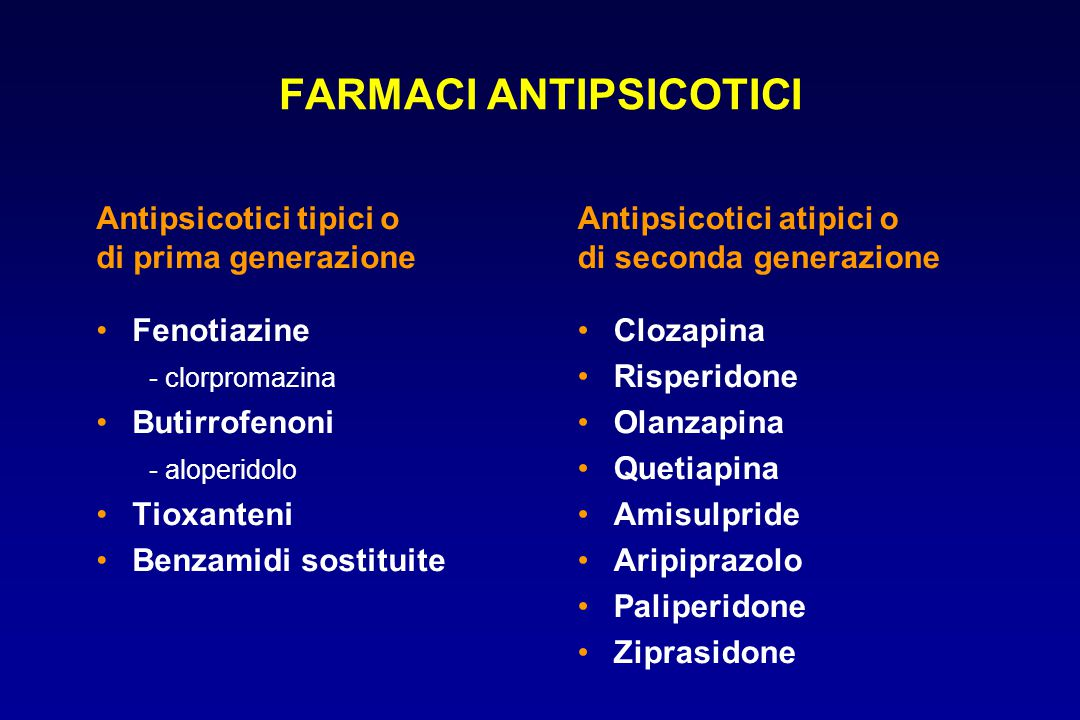
\includegraphics[width=4.78125in,height=3.20833in]{media/image1.jpeg}

\textbf{\emph{TRATTAMENTO DELLA SCHIZOFRENIA:}}

\textbf{\emph{INTRODUZIONE:}}

Possiamo raffigurarci la schizofrenia come un treno che investe la
persona che ne è affetta. L'idea rende perché effettivamente fermare un
treno in corsa non è una delle cose più semplici che si riesce a fare,
così come ad oggi non si riesce a guarire i pazienti affetti da questa
patologia: pensando al treno, riusciamo più che altro ad indirizzarlo.

A differenza di quanto detto sulla depressione e il disturbo bipolare la
schizofrenia è una malattia ad andamento cronico.

Per quanto riguarda le due precedenti patologie il problema principale è
che si riesce a trattare l'episodio acuto ma non c'è garanzia di evitare
le ricadute. Qui invece si può ottenere un miglioramento ma non una
remissione completa dei sintomi, quindi l'ottica è completamente
diversa.

L'esito previsto per questi pazienti è quindi ottenere il massimo
possibile alle condizioni permesse da questo disturbo.

Il trattamento della schizofrenia ha come punto cardine l'utilizzo dei
\textbf{farmaci antipsicotici}, per cui è essenzialmente una
\textbf{\emph{farmacoterapia}}, ma un piano terapeutico appropriato
dovrebbe includere anche approcci psicoterapeutici, psicosociali e
riabilitativi, stabiliti di volta in volta in base alla risposta e a
progressi del paziente stesso. Nelle forme di schizofrenia catatonica,
inoltre, si può ricorrere anche all'uso della \textbf{\emph{terapia
elettroconvulsivante}}.

\begin{itemize}
\item
  \textbf{\emph{Trattamento Farmacologico}}
\end{itemize}

A tutt'oggi il trattamento di prime linea per la schizofrenia è quello
farmacologico, e si avvale essenzialmente degli \emph{antipsicotici},
suddivisi in \textbf{tipici} (noti anche come neurolettici, o
tranquillanti maggiori, che sono dei bloccanti dei recettori
D\textsubscript{2}) e \textbf{atipici} (di più recente sviluppo, sono
degli inibitori dei recettori 5-HT\textsubscript{2} ).

\begin{enumerate}
\def\labelenumi{\arabic{enumi}.}
\item
  Gli \textbf{\emph{antipsicotici tipici}} agiscono principalmente a
  livello della via dopaminergica mesolimbica, la cui iperattività si
  presuppone sia alla base dei \emph{sintomi positivi}, che
  effettivamente rispondono in genere bene agli antipsicotici tipici, i
  quali, dal punto di vista farmacodinamico, possono essere suddivisi
  in:
\end{enumerate}

\begin{itemize}
\item
  \textbf{composti a bassa potenza} (\emph{tioridarina} e
  \emph{clorpromaziza}),
\item
  \textbf{ad alta potenza} (\emph{aloperidolo}, \emph{flufenazina}) in
  base all'affinità di legame coi recettori dopaminergici.
\end{itemize}

\begin{enumerate}
\def\labelenumi{\arabic{enumi}.}
\item
  Gli \textbf{\emph{antipsicotici atipici}}, invece, si differenziano
  dai neurolettici per il loro diverso profilo clinico e tossicologico,
  ed hanno anche una maggior specificità d'azione nei confronti dei
  \emph{sintomi negativi}, potendo agire anche in soggetti che si sono
  precedentemente rivelati resistenti ai neurolettici.

  Gli antipsicotici atipici, inoltre, visto che non interagiscono con la
  trasmissione dopaminergica, \emph{non danno gli effetti collaterali di
  tipo extrapiramidale} tipici degli antipsicotici tipici, e risultano
  quindi meglio tollerati, garantendo una maggior compliance da parte
  del paziente.
\end{enumerate}

Il trattamento farmacologico della schizofrenia è strutturato in 3 fasi
principali:

\begin{itemize}
\item
  \textbf{Fase Acuta}, che è volta al \emph{controllo dei sintomi
  dell'episodio psicotico acuto}, e che ha una durata media di \emph{6-8
  settimane};
\item
  \textbf{Fase di Stabilizzazione}, che consente nel \emph{proseguimento
  della cura a dosi piene per almeno 6 mesi}, così da consolidare i
  risultati ottenuti;
\item
  \textbf{Fase di Mantenimento}, finalizzata alla \emph{profilassi delle
  ricadute e la cui durata varia da 1 a 5 anni o più}.
\end{itemize}

\textbf{Fase Acuta}: In genere nella fase acuta si utilizzano dei
\textbf{neurolettici ad elevata potenza}, come l'\emph{aloperidolo} a
dosi di 10-15 mg/die, oppure si possono usare degli
\textbf{antipsicotici atipici}, come il \emph{risperidone} (4-6 mg/die),
l'\emph{olanzapina} (10-20 mg/die) o la \emph{quetiapina} (400-800
mg/die).

Negli ultimi anni, le linee guida internazionali hanno preso a
raccomandare gli antipsicotici atipici come farmaco di prima scelta per
le fasi acute, sia come alternative ai neurolettici in pazienti con
suscettibilità a sviluppare effetti collaterali gravi o intollerabili.

Se dopo 3 settimane di trattamento il paziente mostra una risposta
parziale è opportuno proseguire la cura, eventualmente aumentando le
dosi, per altre 6 settimane prima di cambiare il farmaco, mentre è bene
sostituirlo subito se non si ha un miglioramento apprezzabile dopo 2
settimane.

Nei pazienti con \emph{elevata componente ansiosa ed agitazione
psicomotoria} è invece opportuno \emph{associare un neurolettico a bassa
potenza} (ad esempio la clorpromazina 100-300 mg/die) ad una
\emph{benzodiazepina} (lorazepam 7,5-12,5 mg/die).

Si definiscono propriamente ``\textbf{resistenti}'' alla terapia quei
pazienti che hanno portato a termine almeno tre periodi di trattamento
negli ultimi 5 anni con tre antipsicotici diversi, appartenenti a due
classi chimiche diverse, con almeno 6 settimane a dosaggio adeguato, e
senza una scomparsa dei sintomi. In questi casi è opportuno passare alla
\textbf{\emph{clozapina}}, l'antipsicotico più efficace al momento
disponibile, il cui uso deve però essere attentamente controllato,
perché il farmaco può causare un'agranulocitosi potenzialmente letale
nell'1-2\% dei pazienti.

Altre strategie per la fase acuta consistono nell'\emph{associazione di
antipsicotici e stabilizzanti dell'umore o benzodiazepine}, anche se
l'efficacia di tali terapie farmacologiche di associazione non è stata
ancora valutata nei dettagli. In caso di comparsa di sintomi
extrapiramidali, più comuni con i neurolettici, si può tentare ad
aggiungere un \textbf{farmaco anticolinergico} (orfenadrina 50-150
mg/die, oppure triesifenidile 2-6 mg/die), mentre se il sintomi
predominante è l'acatisia è utile l'aggiunta di un \textbf{β-bloccante}.

\textbf{Fase di Stabilizzazione}: Consiste nel \emph{proseguimento della
terapia prescritta per la fase acuta}, avendo cura di adattarlo, se
necessario, alle condizioni del paziente tramite aggiunta di farmaci di
associazioni o modificando leggermente le dosi.

\textbf{Fase di Mantenimento}: Una volta raggiunta la stabilità nei
sintomi è necessario formulare un programma terapeutico a lungo termine,
che includa trattamenti farmacologici, psicoterapeutici ed interventi di
tipo riabilitativo psicosociale, così da prevenire le ricadute e
migliorare la qualità della vita.

\begin{itemize}
\item
  \textbf{\emph{Terapia Elettroconvulsivante}}
\end{itemize}

L'impiego della \textbf{terapia} \textbf{elettroconvulsivante}
(\textbf{TEC}) è ad oggi limitato ai casi in cui è presente una marcata
componente affettiva (depressione secondaria o disturbo
schizoaffettivo), nelle forme catatoniche e, in associazione ai farmaci,
nei casi resistenti al solo trattamento farmacologico.

\textbf{\emph{EVOLUZIONE DELLA TERAPIA:}}

\includegraphics[width=5.10069in,height=3.82552in]{media/image2.jpeg}

Dal punto di vista storico, i primi studi sugli antipsicotici risalgono
agli \textbf{anni '60}, quando nel 1952 in Francia si vide che la
\textbf{clorpromazina}, un farmaco usato come ipotermizzante negli
interventi chirurgici, si rivelò dotata di una buona azione
antipsicotica, e a seguito di tale scoperta vennero poi identificate
anche altre molecole ad azione analoga, che vennero generalmente
indicate come \emph{neurolettici.}

I farmaci antipsicotici fin qui scoperti, detti in seguito
\textbf{\emph{antipsicotici tipici}}, si rivelarono in effetti efficaci
nel trattamento dei sintomi positivi, ma erano molto meno efficaci nel
trattamento di quelli negativi, nei confronti dei quali si rivelarono
molto utili altri composti, successivamente denominati
\textbf{\emph{antipsicotici atipici}}, il cui prototipo era la
\textbf{clozapina}, un farmaco scoperto già negli \textbf{anni '70}, ma
che era stata abbandonata nel momento in cui era apparso il suo
principale effetto collaterale, una grave forma di agranulocitosi
potenzialmente mortale.

Sul \textbf{finire degli anni '80} si è visto che in un 30\% dei
pazienti il blocco dei soli recettori D2 non aveva alcun effetto e
risultavano insensibili alla terapia nonostante si aumentassero le dosi
(es. dosi di Aloperidolo da 300 mg/die su un range normale di 4 -- 20
mg): l'unica evidenza era un peggioramento degli effetti collaterali.

Due farmacologi clinici americani iniziarono quindi a sperimentare sui
pazienti \emph{non responders} ad una dose di farmaco per un totale
equivalente di 1000 mg di Clorpromazina in 6 settimane (cioè la dose
totale assunta in questo lasso di tempo). Crearono due farmaci di classe
chimica differente

\begin{itemize}
\item
  Fenotiazine
\item
  Butirrofenoni
\end{itemize}

Non risposero comunque, mantenendo un punteggio elevato nella scala di
sintomatologia che era stata creata. Dopodichè si è provato a testarli
con un 60 mg di Aloperidolo per 6 settimane. Migliorava il 4\% di quelli
trattati con Clorpromazina, mentre il 20\% di quelli trattati con
l'Aloperidolo.

\textbf{All'inizio degli anni '90} riemerge la Clozapina proprio perché
avendo un'attività a così ampio spettro riusciva ad essere efficace nei
pazienti in cui nient'altro funzionava, era efficace nel trattamento di
quelle forme psicotiche che erano invece refrattarie alla terapia con
altri composti tipici. Per tali motivi, ed anche per il fatto che il
rischio relativo di agranulocitosi nella popolazione europea fu stimata
attorno allo 0,7\% (più alta nei soggetti provenienti dal Nord Europa),
si decide si consentire l'uso della clozapina nel trattamento dei
disturbi psicotici, ponendo però come precauzione un esame
emocromocitometrico ogni settimana nei primi 4 mesi, poi una volta al
mese.

La pubblicità di questo farmaco era \emph{``Jack is back''} con
l'immagine di Jack che tornava a lavorare.

La realtà non è proprio così, nel senso che l'efficacia era di avere un
qualche tipo di effetto dove nient'altro aveva funzionato: si sa che
questo non coincide con la guarigione.

\textbf{Nei primi anni 2000,} infine, sono stati scoperti altri farmaci
antipsicotici atipici, oggi definiti ``\textbf{\emph{di seconda
generazione}}'', i quali, come la \textbf{clozapina}, danno generalmente
\emph{minori effetti extrapiramidali}, danno un \emph{minor aumento
della concentrazione della prolattina} ed agiscono principalmente da
\emph{antagonisti dei recettori 5-HT\textsubscript{2}},ad esempio il
\textbf{risperidone} \emph{,}l'\textbf{amilsulipiride},
l'\textbf{aripiprazolo}.

Un problema di questa evoluzione farmacologica sono stati i costi,
perché da un costo medio di 50 dollari all'anno per un paziente trattato
con aloperidolo si è passati ai 9000 per la Clozapina, a cui si
aggiungevano gli emocromi tutte le settimane per le prime 48.

L'Olanzapina non dà agranulocitosi e aveva un costo di 6500 dollari
l'anno.

E' giustificato spendere tanto di più se un farmaco ci dà di più. Mentre
per la Clozapina non ci sono dubbi, per gli altri la situazione è da
valutare tant'è che nel 2000 uscì un editoriale sul British Medical
Journal dal titolo ``il gioco non vale la candela''.

Ad oggi uno studio riporta i risultati dell'efficacia del trattamento di
5 farmaci diversi, di prima e di seconda generazione: la prima cosa che
emerge è che si ottiene lo stesso miglioramento con tutti i farmaci
(Clozapina esclusa).

\emph{\textbf{Efficacy}}: risultati ottenuti tramite Clinical Trial, con
controlli elevati

\emph{\textbf{Effectivness}}: dati ottenuti dalla pratica clinica in
condizioni sperimentali meno controllate ma comunque indicative.

\textbf{\emph{ANTIPSICOTICI TIPICI (``NEUROLETTICI'')}}

Gli \textbf{\emph{antipsicotici tipici}} sono noti anche come
\emph{tranquillanti maggiori} o \emph{neurolettici} a causa dell'effetto
collaterale da blocco dopaminergico che si manifesta con tremori e
sintomi extrapiramidali.

Quindi il termine ``neurolettico'' è stato dato perché questi farmaci
avevano la funzione di ridurre l'attività neuronale, non scevri però da
effetti collaterali.

Inizialmente l'Indicazione terapeutica era somministrare e aumentare le
dosi del farmaco finché non si manifestavano i tipici effetti
collaterali, quali tremore e ipotensione, sintomi extrapiramidali etc.
Questo significa che l'attività terapeutica diventava inscindibile
dall'effetto collaterale.

\emph{\emph{Classificazione:}}

Questi composti possono inoltre essere suddivise in diverse classi
chimiche, tra cui bisogna ricordare le principali:

\begin{itemize}
\item
  \textbf{Fenotiazine}, a loro volta suddivise in \emph{fenotiazine
  alifatiche} (clorpromazina), \emph{fenotiazine piperidiniche}
  (tioridazina) e \emph{fenotiazine piperaziniche} (flufenazina);
\item
  \textbf{Butirrofenoni}, rappresentati essenzialmente dall'aloperidolo;
\item
  \textbf{Tioxanteni}, come il tiotixene;
\item
  \textbf{Dibenzoxazepine}, come la loxapina.
\end{itemize}

\emph{\emph{Usi clinici:}}

Indipendentemente dalla classe chimica di appartenenza, tutti questi
composti sono efficaci soprattutto sui \emph{sintomi positivi}, mentre
quelli negativi permangono inalterati o possono addirittura peggiorare,
così come possono peggiorare anche i sintomi cognitivi, infatti si
possono riscontrare problemi di memoria immediata e pratica, nonché
delle funzioni cognitive, dell'attenzione e della concentrazione.

Gli antipsicotici tipici, in ogni caso, esercitano un \emph{effetto
antipsicotico}, \emph{sedativo} e \emph{disinibente}, utile soprattutto
nelle manifestazioni autistiche.

\emph{\emph{Profilo molecolare:}}

L'azione comune è il \textbf{blocco dei recettori D2}, che ha portato
evidenze a supporto dell'ipotesi dopaminergica della schizofrenia, e
l'effetto terapeutico si spiega mediante il blocco dei circuiti
mesocorticali e mesolimbiche.

\emph{\emph{Effetti collaterali:}}

L'inevitabile azione anche su:

\begin{itemize}
\item
  \textbf{via tubero-infundibulare} causa \emph{amenorrea} e
  \emph{disfunzioni sessuali} (infatti la dopamina, tramite i sui
  recettori D2, ha un'azione inibitoria nei confronti del rilascio della
  prolattina a livello ipofisario),
\item
  mentre il blocco dopaminergico a \textbf{livello nigro-striatale}
  determina la comparsa degli \emph{effetti extrapiramidali}, che sono
  particolarmente marcati proprio con gli antipsicotici tipici e
  includono:
\end{itemize}

\begin{itemize}
\item
  effetti acuti come:
\end{itemize}

\begin{itemize}
\item
  le \textbf{distonie} a livello del tronco e degli arti, che richiedono
  l'aggiunta di farmaci anticolinergici,
\item
  \textbf{crisi a livello oro-linguale}, che possono dare anche
  contratture molto dolorose, così come torsione dei bulbi oculari verso
  l'alto, e tutte queste manifestazioni acute in genere compaiono entro
  5 giorni dall'inizio del trattamento nel 40-60\% dei pazienti.
\end{itemize}

\begin{itemize}
\item
  Altre forme ad esordio più tardivo sono: il \textbf{parkinsonismo},
  che compare in genere dopo 3-4 mesi, e l'\textbf{acatisia}, che è
  dipendente dal blocco nigro-striatale e consiste nell'impossibilità a
  stare fermi o in una marcata irritabilità, le \textbf{discinesie}
  (\emph{Rabbit Syndrome}: è un tipo particolare di discinesia che imita
  il movimento di masticazione del coniglio), i \textbf{tremori.}

  Per ovviare a parkinsonismo e discinesie, spesso tardive (dopo
  settimane o mesi di trattamento) si proponevano le cosiddette
  \emph{\textbf{drug holidays}}, cioè una sospensione del farmaco
  temporanea proprio per attenuare queste manifestazioni. Se non era il
  medico a prescriverle erano comunque i pazienti stessi perché la
  situazione diventava ingestibile. Il problema era che deliri e
  allucinazioni ricomparivano molto rapidamente, con un tasso di
  ricaduta del 10\% che aumentava di mese in mese.
\end{itemize}

\begin{itemize}
\item
  il forte \textbf{blocco sui recettori α\textsubscript{1}, M1 ed H1}
  determina gli effetti collaterali più frequenti, come \emph{nausea},
  \emph{vomito}, \emph{ipotensione ortostatica}, \emph{sedazione} ed
  \emph{incremento dell'intake di cibo}.
\item
  La \textbf{scarsa azione sui recettori 5-HT\textsubscript{2}}
  giustifica l'inefficacia di questi farmaci nei confronti dei sintomi
  negativi,
\end{itemize}

\emph{\emph{Capostipite:}}

Il capostipite degli antipsicotici tipici è
l'\textbf{\emph{aloperidolo}}, un potente bloccante dei recettori D2
mesocorticali e un poco attivo anche sui recettori
5-HT\textsubscript{2A} e 5-HT\textsubscript{1A}, oltre al consueto
blocco sui recettori α\textsubscript{1}, M1 ed H1.

Accanto alla classe dei neurolettici vennero poi proposte anche altre
classi farmacologiche, come quella dei cosiddetti \emph{farmaci
incisivi} (che agivano cioè prevalentemente sui sintomi positivi), i
\emph{farmaci sedativi} (usati per l'effetto tranquillante) ed i
\emph{farmaci ad azione disinibente}, cioè che cercavano di contrastare
l'isolamento del paziente, ma oggi questa tutte queste distinzioni sono
state abolite, preferendo basarsi solo sul profilo d'azione molecolare
del composto e della classe chimica a cui appartiene.

Sino agli '70-'80 non era ancora ben chiaro il meccanismo d'azione dei
farmaci antipsicotici, che divenne poi chiaro risiedere
nell'\textbf{\emph{antagonismo dei recettori D2}}, per cui nei primi
periodi furono proposte diverse terapie di associazione, in cui si
cercava di combinare (in genere senza risultati soddisfacenti) più
antipsicotici diversi, nella speranza di ottenere risultati migliori a
fronte di effetti collaterali minori. Dalla fine degli anni '80, e poi
decisamente dai primi anni '90, si scelse si sostituire il termine
``neurolettico'' con ``\emph{antipsicotico}'', così da separare, almeno
dal punto di vista semantico, l'effetto terapeutico da quello
collaterale

\textbf{\emph{ANTIPSICOTICI ATIPICI:}}

Col tempo si è cercato di scindere l'effetto terapeutico da quello
collaterale e quindi si è preferito il termine antipsicotici a quello
neurolettici per indicare il cambio d'indirizzo terapeutico, ottenuto a
partire dagli anni '90 con quelli di 2° generazione. Si cercò di mettere
a punto farmaci con minori effetti collaterali, che non rendevano più
necessario cercare l'effetto collaterale per capire l'efficacia del
farmaco, e questo perché si comprese che l'effetto farmacologico
desiderato compariva quando venivano bloccati circa i \emph{2/3 dei
recettori D2} presenti a livello cerebrale, e al di sopra di tale valore
oltre all'effetto farmacologico comparivano gli effetti extrapiramidali,
per cui si riuscì finalmente a stabilire un dosaggio più preciso ed
efficace, capace di bloccare esattamente il 65-70\% circa dei recettori
D2, abbandonando le dosi eccessivamente elevate che avevano
caratterizzato il periodo precedente.

Gli \textbf{\emph{antipsicotici atipici}}, dimostrarono un'efficacia
anche nei confronti dei \emph{sintomi negativi} e creano minori
problematiche di natura cognitiva e minori effetti collaterali.

\emph{\emph{Classificazione: }}

Dal punto di vista chimico, gli antipsicotici atipici appartengono alla
classe:

\begin{itemize}
\item
  delle \textbf{dibenzoazepine} (come la clozapina),
\item
  dei \textbf{benzisossazoli} (come il risperidone)
\item
  delle \textbf{tienobenzodiazepine} (come l'olanzapina).
\end{itemize}

\emph{\emph{Capostipite:}}

Il capostipite degli antipsicotici atipici, nonché il farmaco più
efficace di tutta la categoria, che agisce soprattutto tramite un blocco
sui recettori 5-HT\textsubscript{2A}, soprattutto in sede prefrontale, è
la \textbf{\emph{clozapina}}.

\emph{\emph{Effetti collaterali di Clozapina:}}

Gli antipsicotici atipici hanno minori effetti collaterali
extrapiramidali per via del \emph{ridotto effetto di blocco
dopaminergico}, ma conservano tuttavia i loro effetti sui
\emph{recettori α\textsubscript{1}, M1 ed H1.}

Gli effetti collaterali della clozapina includono:

\begin{itemize}
\item
  un'\textbf{agranulocitosi} che si caratterizza per \emph{neutropenia}
  (neutrofili al di sotto delle 500 unità/mm\textsuperscript{3}) e
  \emph{leucopenia} (con leucociti al di sotto delle 3500
  unità/mm\textsuperscript{3}).

  A tutt'ora il rischio di questa complicazione ha una probabilità
  stimata attorno allo \textbf{0,7\%}, (prima era del 2\% circa). Questo
  rischio impone di \emph{fare settimanalmente un emocromo}, almeno nei
  primi 4 mesi di terapia, e nel momento in cui si osservasse la
  neutropenia si deve immediatamente sospendere il farmaco, e così
  facendo la percentuale di sviluppo di agranulocitosi grave è
  sovrapponibile a quella di qualsiasi altro antipsicotico.

  Come regola generale questo farmaco è per definizione di seconda
  scelta, da usare solo per forme gravi e resistenti agli altri
  antipsicotici, e la si usa in pazienti non responders che abbiano già
  provato con almeno due altri farmaci appartenenti a classi
  farmacologiche diverse.

  Il problema dell'agranulocitosi, peraltro, è un \emph{disturbo su base
  immunitaria}, ed è quindi un grave problema, perché anche se si prova
  a somministrarla anche a distanza di tempo il problema si ripresenta,
  anzi tende ad aumentare sempre più.

  Fattori di rischio per lo sviluppo di questo effetto collaterale sono
  l'\emph{età avanzata}, il \emph{sesso} \emph{femminile}, una certa
  \emph{predisposizione genetica} e possibili \emph{fattori tossici o
  autoimmuni}.

  N:B: Una cosa da tenere sempre a mente, tuttavia, è che non si deve
  \textbf{\emph{mai associare la clozapina col litio}}, che già di per
  sé può causare una leucocitosi, tanto che si può avere una leucopenia
  inapparente nelle prime 2 settimane, ed alla terza settimana le
  conseguenze possono essere già molto gravi.
\item
  In virtù del \emph{blocco D2} a livello tubero-infundibulare, inoltre,
  si sviluppa \textbf{iperprolattinemia}, soprattutto a seguito di un
  precedente trattamento con \emph{risperidone} o \emph{amilsulpiride};
  questa iperprolattinemia è dose-dipendente:

  nelle donne causa tensione mammaria, galattorrea ed amenorrea,

  nei maschi causa sempre tensione mammaria, galattorrea, riduzione
  della libido, impotenza e ginecomastia, ma non ha effetti cancerogeni.
\item
  Il \emph{blocco dei recettori α\textsubscript{1}}-adrenergici causa
  \textbf{ipotensione ortostatica},
\item
  L'azione di \emph{blocco dei recettori H1} dà \textbf{sedazione} e
  \textbf{incremento ponderale},
\item
  Il \emph{blocco sui recettori M1} dà \textbf{sintomi cognitivi}, come
  disturbi dell'attenzione, della concentrazione e della memoria, ma
  hanno effetti anche sull'apparato gastro-intestinale, come il
  \textbf{rallentamento della peristalsi}, con \textbf{stipsi}, nonché
  \textbf{secchezza delle} \textbf{fauci}, \textbf{glaucoma},
  \textbf{ipertrofia prostatica}, \textbf{tachicardia}.
\item
  Altri effetti collaterali legati alla clozapina sono l'\textbf{aumento
  delle transaminasi epatiche}, \textbf{scialorrea}, \textbf{aumentata
  sudorazione}
\item
  Ad alto dosaggio, \textbf{crisi convulsive}.
\item
  I \textbf{problemi a livello cardiologico} sono comuni a tutti gli
  antipsicotici, in particolare si può avere un \textbf{allungamento del
  tratto QT}, soprattutto con la clozapina ed alcuni nuovi composti,
  come la quetiapina, per cui è consigliato un monitoraggio con ECG
  all'inizio della terapia ed uno dopo 15 giorni con calcolo
  dell'eventuale variazione rispetto alla registrazione precedente.
  Fattori di rischio per l'allungamento del tratto QT sono il
  \emph{sesso femminile}, l'\emph{ipokaliemia} e le \emph{sindromi
  congenite del QT lungo}, dovute a mutazioni dei canali del
  K\textsuperscript{+} o del Na\textsuperscript{+}.
\item
  Una particolare manifestazione dovuta alla clozapina è poi la
  \textbf{\emph{sindrome maligna da neurolettici}}, che è causata anche
  da altri antipsicotici: l'evoluzione di questa condizione è mortale
  nel 20\% dei casi se non trattata, ma se è riconosciuta subito e
  trattata non ha complicanze gravi.

  La sindrome si manifesta nello 0,2-0,4\% dei pazienti trattati con
  antipsicotici, ed è più frequente con gli antipsicotici di I
  generazione e di elevata potenza, caratterizzandosi per:
\end{itemize}

\begin{itemize}
\item
  \emph{rialzo termico},
\item
  \emph{rigidità muscolare},
\item
  squilibrio del sistema neurovegetativo con \emph{tachicardia},
  \emph{tachipnea}, \emph{disfagia}, \emph{ipotensione},
  \emph{sudorazione profusa} e talvolta anche \emph{ipertensione
  diastolica}. I
\end{itemize}

\begin{quote}
l paziente si presenta immobile, rigido, con una contrattura di tipo
spastico, in una condizione di stupore, ed è scarsamente reattivo,
talora confuso. La contrattura porta ad un incremento plasmatico di CPK,
delle transaminasi, dell'aldolasi, dell'LDH ed anche della mioglobina,
con conseguente \emph{mioglobinuria} ed \emph{insufficienza renale}.

Questi pazienti devono essere trattati, essendo la patogenesi legata ad
un blocco dopaminergico a livello ipotalamico, con \textbf{agonisti
dopaminergici} come la \emph{bromotriptina} oppure, siccome prevale la
contrattura a livello periferico muscolare, con dei \textbf{chelanti del
calcio}, come il \emph{nantrolene sodico}, somministrato a dosi di 1-2
mg per via endovenosa, oltre al posizionamento di un sondino
naso-gastrico, perché questi pazienti non si alimentano spontaneamente.
È fondamentale diagnosticare questa sindrome per tempo, in quanto i
pazienti possono morire per insufficienza renale, TEP o per
insufficienza renale.
\end{quote}

\emph{\emph{Altri antipsicotici atipici:}}

Nei primi anni 2000, infine, sono stati scoperti altri farmaci
antipsicotici atipici, oggi definiti ``\textbf{\emph{di seconda
generazione}}'', i quali, come la \textbf{clozapina}, danno generalmente
minori effetti extrapiramidali, danno un minor aumento della
concentrazione della prolattina ed agiscono principalmente da
\emph{antagonisti dei recettori 5-HT\textsubscript{2}}:

\begin{itemize}
\item
  il \textbf{risperidone} \emph{ad alte dosi può dare sintomi
  extrapiramidali rilevanti},
\item
  l'\textbf{amilsulipiride} \emph{blocca i recettori D2 piuttosto che i
  5-HT\textsubscript{2}}.
\item
  Caso particolare è rappresentato dall'\textbf{aripiprazolo},
  commercializzato col nome di Abilify, che è un \emph{agonista parziale
  dei recettori D2}, dai cui studi è emerso che la schizofrenia non sia
  dipendente solo da un aumento della dopamina, ma anche dalla presenza
  di un difetto localizzato corticale che funge da ``primus movens'' a
  livello mesolimbico e mesocorticale per l'aumento dopaminergico,
  quindi, almeno a livello teorico se si agisse con un farmaco, come un
  agonista parziale si potrebbe ottenere un miglior bilanciamento tra
  aree con minore e maggiore presenza di neurotrasmettitore rispetto al
  normale, anche se attualmente questo meccanismo farmacologico, sul
  piano clinico, si è rivelato poco efficace.
\end{itemize}

\textbf{\emph{FARMACODINAMICA E FARMACOCINETICA DEGLI ANTIPSICOTICI}}

\emph{\emph{Farmacodinamica}}

Per quanto riguarda il profilo farmacodinamico degli antipsicotici, il
composto che sino ad oggi ha dimostrato un'\emph{efficacia maggiore è la
\textbf{clozapina}}, la quale tuttavia ha anche notevoli effetti
collaterali, per cui viene in genere riservata per disturbi psicotici
gravi e non responsivi ad altri farmaci, i quali hanno peraltro più o
meno lo stesso livello di efficacia. In realtà si deve precisare che
questi farmaci, anche se in grado diverso, funzionano sempre, infatti
nella fase acuta i pazienti migliorano nel 50-60\% dei casi e le
ricadute sono minori nel momento in cui il paziente viene trattato più a
lungo possibile con dosi basse. Per quanto riguarda invece la potenza,
essa viene espressa come la dose capace di determinare un certo effetto,
quindi a parità di effetto desiderato, a dosi minori corrisponde una
potenza maggiore rispetto ad un farmaco che ottiene il medesimo effetto
ma a dosi più elevate. L'\textbf{aloperidolo} è l'\emph{antipsicotico
con maggior potenza}, quindi è il più antidopaminergico, ma anche un
bloccante dei recettori H1 ed M1, per cui sulla base della potenza si
possono anche prevedere i possibili effetti collaterali.

\emph{\emph{Farmacocinetica:}}

Dal punto di vista farmacocinetico, alcuni antipsicotici hanno un
\emph{assorbimento rapido e completo}, come nel caso
dell'\textbf{aloperidolo}, per altri, come la \textbf{clorpromazina},
l'assorbimento è \emph{lento ed incompleto} se somministrata per via
orale. Ovviamente, se l'antipsicotico viene somministrato invece per via
parenterale la concentrazione efficace è raggiunta molto più
rapidamente, e gli effetti sedativi tendono anch'essi a manifestarsi più
precocemente, tanto che in passato si sfruttava tale fenomeno per
indurre una ``\emph{tranquillizzazione rapida}'' nei pazienti agitati.
Molto utili sono poi le ``\textbf{\emph{formulazioni depot}}'', cioè
somministrazioni di antipsicotico in veicolo oleoso, in modo da dare una
lenta liberazione del composto a partire dal sito di somministrazione,
garantendone così una concentrazione stabile in periodi relativamente
lunghi, e questa strategia viene tipicamente messa in atto in pazienti
poco complianti, che faticano ad assumere giornalmente l'antipsicotico
per via orale.

\textbf{\emph{PROFILO MOLECOLARE:}}

Dal punto di vista del profilo molecolare, tutti i farmaci
antipsicotici, ma in particolare i \textbf{\emph{neurolettici,}}
agiscono da \textbf{antagonisti recettoriali D2}, ma interagiscono anche
con altri tipi di recettori:

\begin{itemize}
\item
  \emph{recettore M1} dell'acetilcolina, in particolare la
  \textbf{tioridazina} (dà una \emph{sedazione} e un'\emph{ipotensione
  ortostatica} relativamente marcata se confrontata col suo effetto
  terapeutico) e la \textbf{clorpromazina} (causa una \emph{marcata
  sedazione} e \emph{ipotensione ortostatica}, a fronte di un'attività
  antipsicotica ed effetti extrapiramidali minori)
\item
  \emph{recettore H1} dell'istamina la \textbf{clozapin}a e la
  \textbf{clorpromazina }
\item
  \emph{recettore α\textsubscript{1} adrenergico} la clorpromazina.
\end{itemize}

L'\textbf{aloperidolo} e la \textbf{pimozide}, ad esempio, hanno una
\emph{marcata azione antipsicotica con scarsi effetti sulla pressione e
scarsa sedazione}, sebbene possano dare anche \emph{effetti collaterali
extrapiramidali con relativa facilità}.

Gli \textbf{\emph{antipsicotici atipici}}, invece, si caratterizzano per
il fatto di agire principalmente come \textbf{bloccanti dei recettori
5-HT\textsubscript{2}} piuttosto che da antagonisti dei recettori D2,
anche se possono comunque interagire con gli altri tipi di recettori.

Ad esempio:

\emph{Recettore M\textsubscript{1} e alfa \textsubscript{1}} agisce la
\textbf{clozapina}, è l'antipsicotico con efficacia maggiore, ma è anche
uno di quelli con effetti collaterali più marcati, infatti può dare
\emph{forte sedazione ed ipotensione ortostatica}, anche se è
generalmente \emph{priva di effetti collaterali extrapiramidali}.

\emph{Recettore H 1} quindi per quanto riguarda quindi l'aumento
ponderale, lo si ha soprattutto con \textbf{l}a \textbf{clozapina} e
l'\textbf{olanzapina},

\textbf{\emph{EFFETTI GENERALI DEGLI ANTIPSICOTICI:}}

\textbf{Blocco dei Recettori D2}, che agisce a livello di diversi
circuiti cerebrali:

\begin{itemize}
\item
  \emph{Blocco Nigro-Striatale}, determina gli \textbf{effetti
  collaterali extrapiramidali}, come il \emph{parkinsonismo}, le
  \emph{discinesie} (movimenti involontari che coinvolgono soprattutto
  la muscolatura periorale e linguale, con protrusione e rotazione, che
  compaiono dopo alcune settimane) e l'\emph{acatisia} (il paziente non
  riesce a stare fermo, e non vi sono solo sintomi motori ma anche
  irrequietezza, agitazione e frenesia). Fino agli anni '90, per il
  trattamento di questi disturbi si associava agli antipsicotici un
  \emph{farmaco anti-colinergico} prima ancora che il sintomo
  comparisse, ma ciò riduceva l'assorbimento intestinale di altri
  farmaci. Altri effetti extra-piramidali sono poi le \emph{distonie
  acute}, cioè contrazioni involontarie improvvise e dolorosissime che
  possono comparire anche a dosi molto basse, e che sono essenzialmente
  dovute a delle reazioni di ipersensibilità, e le \emph{discinesie
  tardive}, che insorgono dopo alcuni mesi e sono molto disturbanti,
  tanto da richiedere spesso l'interruzione della terapia. Negli USA, in
  passato, per cercare di prevenire e trattare queste manifestazioni per
  nulla piacevoli, si era soliti mettere in atto delle
  ``\emph{drug-holidays}'', ovvero periodi di sospensione della terapia,
  nel tentativo di ridurre la discinesia tardiva, anche a fronte di un
  peggioramento del quadro psichico. Oggi, in genere, non si ricorre più
  a simili strategie, poiché si è visto che basta adeguare meglio la
  dose per ridurre al minino il rischio di effetti extrapiramidali, i
  quali non possono comunque essere del tutto evitati.
\item
  \emph{Blocco Ipotalamo-Ipofisario}, con interferenza a livello della
  via tubero-infundibolare, che determina \emph{ginecomastia,
  galattorrea, impotenza ed amenorrea} per \textbf{iperprolattinemia.}
\item
  \emph{Blocco Mesolimbico-Frontale}, che determina diversi
  \textbf{sintomi cognitivi}, tuttavia si è visto che il miglioramento
  clinico del paziente portava poi al superamento di questi problemi
  cognitivi, che sono probabilmente legati al ``reset'' dell'attività
  mesolimbica-frontale.
\end{itemize}

\textbf{Blocco dei Recettori α\textsubscript{1}}, che causa
\emph{ipotensione ortostatica}.

\textbf{Blocco dei Recettori M1}, che determina la comparsa di sintomi
cognitivi quali \emph{disturbi dell'attenzione}, \emph{della
concentrazione e della memoria}, con effetti anche sull'apparato
gastro-intestinale, quali \emph{rallentamento della peristalsi},
\emph{stipsi} e \emph{secchezza della fauci}, ma non bisogna dimenticare
che il blocco M1 può peggiorare una condizione di \emph{glaucoma} o di
\emph{ipertrofia prostatica}, nonché determinare \emph{tachicardia} ed
\emph{allungamento del tratto QT}.

\textbf{Blocco dei Recettori H1}, a cui segue \emph{aumento
dell'appetito} e \emph{sedazione}, la quale era un tempo sfruttata per
la gestione di pazienti molto agitati, anche se oggi si preferisce
piuttosto associare una benzodiazepina ad un antipsicotico, per cui
l'effetto sedativo da blocco H1 è diventato essenzialmente un effetto
collaterale, che può anche scoraggiare il paziente dal continuare la
cura.

\textbf{Blocco dei Recettori 5-HT}, che è il meccanismo d'azione
principale degli antipsicotici atipici, ma può anche causare un
\emph{notevole aumento ponderale}.

\textbf{Effetti Cardio-Vascolari}, come la \textbf{\emph{sindrome da QT
lungo}}, che predispone alla \emph{torsione di punta}, alla
\emph{fibrillazione ventricolare} ed alla \emph{morte improvvisa}, per
cui è necessario monitorare il paziente con ECg sia prima che durante la
terapia, soprattutto in pazienti affetti da sindrome metabolica e DMT2.

\textbf{Aumento dell'Appetito}, legato al blocco dei recettori H1, D e
5-HT, e che può aggravare o scompensare una condizione di DMT2 o di
sindrome metabolica, ed i farmaci che mostrano maggiormente questo
effetto collaterale sono l'\emph{olanzapina} e la \emph{clozapina}.

\emph{\textbf{MORTALITÀ DEI PAZIENTI SCHIZOFRENICI}:}

I pazienti schizofrenici hanno una probabilità aumentata di morire per
cause non naturali rispetto alla popolazione generale.

\begin{itemize}
\item
  Rischio di suicidio \textgreater{} 43 volte
\item
  Rischio di morte \textgreater{} 10 volte (in 3 anni) in pazienti che
  non assumevano alcuna terepia rispetto a chi era in cura.
\end{itemize}

\textbf{\emph{Rischio di Suicidio:}}

La Clozapina è quella che riduce in assoluto di più il rischio di morte
per suicidio: il motivo va ricercato nell'azione della
\textbf{serotonina}, che bocca la dopamina. Bloccando la serotonina
aumenta la dopamina (ma non a livello del mesolimbico) che blocca a sua
volta la produzione di prolattina a livello del tubero infundibolare. A
livello piramidale e frontale si ipotizza invece che la dopamina venga
aumentata, e questo è il motivo per cui questi farmaci migliorano le
funzioni cognitive.

L'azione serotoninergica riduce l'aggressività e il rischio suicidario,
motivo per cui questi farmaci si usano anche in altre patologie: l'unico
``\emph{marker}'' del rischio suicidario che abbiamo identificato finora
è proprio la serotonina che viene trovata alterata in tutti i pazienti
deceduti per questo motivo.

\emph{\textbf{Aumento del peso corporeo}:}

I pazienti schizofrenici vivono generalmente \emph{15-20 anni in meno
rispetto alla popolazione generale}, e questo soprattutto a causa del
loro stile di vita, che tende a diventare sempre più sedentario e con
un'alimentazione disarmonica, a cui va poi aggiunto che spesso, per
motivi ancora non del tutto chiariti, lo schizofrenico è anche
\emph{iperteso}, ed ha una prevalenza di \emph{diabete} che è doppia
rispetto alla popolazione generale.

Gli schizofrenici, in generale, tendono ad essere molto più grassi,
soprattutto dai 25 anni in su, e nel momento in cui cominciano ad
assumere gli antipsicotici questo incremento ponderale si fa ancor più
evidente, arrivando ad accumulare anche 10-15 Kg in un solo anno.

Tutto questo accade soprattutto con la \emph{clozapina}, meno col
risperidone, mentre il rischio è quasi nullo con lo ziprasidone, anche
se non bisogna dimenticare il possibile aumento del colesterolo e dei
trigliceridi che porta ad un aumentato rischio di aterosclerosi.

Gli antipsicotici favoriscono l'aumento ponderale tramite diversi
meccanismi, in primis il \textbf{blocco dei recettori H1}, che determina
un \emph{notevole incremento dell'appetito}, così come avviene anche coi
\emph{recettori 5-HT\textsubscript{2C}}, ma molto rilevante è anche
l'aumento dell'\textbf{insulino-resistenza}, che rappresenta il
collegamento tra l'assunzione degli antipsicotici ed il diabete, e si
deve comunque considerare che alla base di tale fenomeno vi sono
probabilmente dei meccanismi genetici, come dimostrato dal fatto che
l'aranzapina favorisce l'incremento ponderale in modo dose-dipendente, e
che il rischio di sviluppare sovrappeso nei pazienti in trattamento con
antipsicotici tipici è triplicato rispetto alla popolazione generale, e
tende ad aumentare ulteriormente con l'uso degli antipsicotici di II
generazione, come appunto l'aranzapina e la clozapina. Il motivo certo
della connessione tra antipsicotici e diabete, in ogni caso, non è
ancora stata ben chiarita, sono state tuttavia fatte diverse ipotesi,
che prendono in considerazione una possibile \emph{azione tossica dei
farmaci sulle isole del Langherans}, una \emph{reazione autoimmune
contro le cellule del pancreas endocrino} o un'\emph{azione diretta nei
confronti dell'insulina}, tale da indurre insulino-resistenza
(quest'ultimo meccanismo è probabilmente il punto centrale).

Questo è un grosso problema clinico perché vi si sommano gli effetti
della malattia, come

\begin{itemize}
\item
  \textbf{scarsa cura di sé}
\item
  \textbf{igiene personale problematica}
\item
  \textbf{insufficiente esercizio fisico }
\item
  \textbf{dieta molto sbilanciata}
\item
  \textbf{fumo, alcol, stile di vita sregolato }
\item
  \textbf{scarsa compliance} (aderenza alla terapia)
\end{itemize}

Sulla \emph{``scarsa cura di sé}'' è stato pubblicato un articolo sul
New England Journal of Medicine che sottolineava come a 35-40 anni la
maggioranza dei pazienti schizofrenici portasse la dentiera come
conseguenza di una mancata igiene personale. Questa è un po' una cartina
tornasole della gravità della patologia che non va di certo ridotta a
deliri e allucinazioni.

Sull'aumento ponderale si può lavorare modificando lo stile di vita e
impostando una dieta che contenga gli eccessi alimentari abbinata ad una
regolare attività fisica. Le prime settimane di trattamento sono
fondamentali da questo punto di vista perché è il periodo in si prendono
chili che si fatica a smaltire dopo. Questi pazienti non riescono a
trattenersi dal mangiare per l'effetto dei farmaci.

Riassumendo per avere una riduzione degli effetti piramidali si ha un
aumento del peso corporeo.

\textbf{\emph{COMPLIANCE DEL PAZIENTE AL TRATTAMENTO}:}

Il farmaco con la migliore compliance in assoluto è l'Olanzapina, anche
se purtroppo è quello che dopo la Clozapina causa il maggior aumento di
peso. Questo studio riporta i mesi di terapia che si riescono a portare
avanti senza interruzioni:

\begin{itemize}
\item
  9 mesi Olanzapina
\item
  4 mesi Quetiapina
\item
  3,5 mesi Risperidone
\end{itemize}

Questo è un valore mediano quindi 50\% meno 50\% più di nove mesi.
L'interruzione del trattamento equivale ad una riacutizzazione dei
sintomi.

\emph{\textbf{Caso Clinico}: un paziente seguito al Braga (ingegnere)
picchia la moglie perché questa si sarebbe messa d'accordo con l'amico
dentista e tutta la cerchia dei conoscenti per registrare quello che lui
faceva e diceva per poi prenderlo in giro. Ricoverato e messo sotto
trattamento sintomi scomparsi. Tornato a casa sta bene, pensa che la
terapia sia inutile e la sospende. Riprende il vizio di picchiare la
moglie, viene ripreso e rimesso dentro e si convince a continuare la
terapia. Questo è stato uno dei primi a prendere l'Olanzapina. Seguendo
la terapia non è mai più stato ricoverato ma purtroppo rimane
schizofrenico, viene allontanato dal lavoro con un'invalidità di
malattia e trascorre tutta a vita a fare il genitore disoccupato. }

Ciò significa che si riesce a ridurre il numero dei ricoveri ma non si
riesce a bloccare il resto.

I sintomi positivi ricompaiono tutte le volte che un paziente sospende
il trattamento.

Non seguire una terapia comporta probabilità di essere ricoverati e
peggiora i deficit cognitivi abbreviando l'aspettativa di vita, quindi è
bene ricordare ai familiari l'importanza della terapia.

Ad oggi più che il farmaco è importante la compliance, motivo per cui si
sono creati farmaci da iniettare endovena: la molecola legata ad una
sostanza oleosa si libera nel sangue dal punto di inoculazione per un
periodo di un mese (3 mesi per un nuovo farmaco in fase di studio).
Questo si traduce in una certezza di adesione alla terapia, quindni
minor numero di ricoveri e una notevole riduzione dei sintomi positivi,
in modo che la persona possa trascorrere la maggior parte del suo tempo
a casa e non in ospedale.

\textbf{\emph{SUPPORTO ALLA TERAPIA FARMACOLOGICA}:}

Le terapie alternative come musicoterapia, spor all'aria aperta etc
sembrano molto utili per far passare il tempo al paziente ma non hanno
un grande effetto sul decorso. Farmaci e ambiente sociale sono invece
fondamentali: passare da un atteggiamento di ansia e giudizio negativo
nei confronti del paziente a un tentativo di aiuto, comprensione e
supporto è fondamentale perché viene recepito bene ed influisce
moltissimo su sintomi e ricadute, nonostante la terapia.

Quindi sono persone molto sensibili al clima emotivo: la
\textbf{\emph{psicoeducazione alla famiglia}} è fondamentale e si
compone di soli 12 incontri di 1 -- 1 h e mezza l'uno.

Questo è importante perché in alcuni casi i genitori non riuscendosi a
sintonizzare sul disagio enorme del figlio dicono cose strabilianti come
``\emph{non vuole far niente, non ha interessi oltre il cibo. Spende
tutti i miei e non vuole lavorare}''.

Resta compito del medico far comprendere i vari aspetti della patologia
ai parenti: queste considerazioni sono molto importanti perché
l'atteggiamento della famiglia o del contesto sociale incide molto sul
decorso e sul benessere del paziente. Queste cose è opportuno saperle
perché alla notizia di schizofrenia i familiari si disperano dando la
persona per finita.

\emph{\textbf{Caso Clinico}: Paziente i cui familiari rimangono
sconvolti ricevendo la diagnosi di schizofrenia, basata sul fatto che
questa ragazza sente le voci. La giustificavano come timida e
introversa, una che alle domande rispondeva sempre sì. Ma lasciando
stare allucinazioni ed etichette, chiedendo alle amiche, non si poteva
dire che la paziente avesse la stessa vita degli altri: non usciva più
di casa, non vedeva più nessuno, non ha un moroso e non s'è fatta una
famiglia}.

Un altro aspetto che si sta valutando è far comprendere al paziente come
\textbf{\emph{autogestirsi}} nella vita quotidiana: rispiegare gesti
molto banali come far la spesa o compiere le più semplici attività
quotidiane (skill training) porta a un grande miglioramento.

Si cerca in ultima analisi di evitare che il paziente schizofrenico sia
abbandonato a se stesso per evitare il degrado della persona.

\textbf{\emph{ESITO DELLA TERAPIA:}}

Il funzionamento, inteso come la percentuale di persone che lavorano
nella popolazione generale, è intorno all' 80\%.

Negli schizofrenici negli anni '55 -- 2000 (estendibili al 2015-'16) non
supera il 10 -- 15 \%, con occupazioni minime e protette cioè con una
persona a fianco. Con la terapia ci si aspettava un miglioramneto ma
quello che succede è strano perchè con un nuovo trattamento si dovrebbe
avere un migliore funzionamento dei pazienti affetti, mentre quello che
si nota è una riduzione dell'attività lavorativa.

Si tenga presente che gli antipsicotici di 1° generazione (definiti
\emph{``neurolettici}'' dagli scopritori francesi) sono efficaci su
deliri e allucinazioni, quindi viene spontaneo chiedersi come mai queste
persone, avendo un esordio di malattia intorno ai 22-23 anni per i
maschi (le femmine qualche anno dopo) non riescano a lavorare.

\emph{\emph{Caso Clinico:Paziente del Braga che riceveva come stipedio
un sussidio dall'ospedale per accompagnare un addetto comunale al verde
pubblico a piantare fiori nelle aiole (fiori che di notte venivano
rubati dai nostri amati concittadini, ma questo non ci interessa per la
lezione). Ha fatto questo lavoro per sole due ore, non di certo perché
aveva deliri e allucinazioni. Allora cosa glielo impediva?}}

Si tenga presente che negli anni `50 le condizioni lavorative erano
molto meno competitive e stressanti di adesso, però nonostante 50-60
anni di terapia un paziente affetto da schizofrenia ha questa
probabilità di lavorare.

Dato Americano: circa il 50\% dei pazienti al primo episodio (che
significa il primo attacco acuto, cioè quando emergono per la prima
volta in modo importante deliri e allucinazioni cui segue un ricovero)
hanno ricevuto un'indennità di invalidità e vivono in una casa protetta
entro 6 mesi dall'esordio della loro malattia. Meno del 20\% hanno una
loro casa senza che nessuno li aiuti.

Il motivo è che sostanzialmente i farmaci non riescono ad agire sui
sintomi Negativi, mentre sono molto efficaci su quelli Positivi.
Attualmente non ci sono nuove idee.

Kraeplin definiva la schizofrenia ``\textbf{demenza preacox}'': quella
persona non riesce a vivere come i suoi coetanei, sente di essere
diversa: \emph{``Io non ho una famiglia, non ho un lavoro e non sono
come gli altri''.} Lui stesso definiva deliri e allucinazioni come
sintomi accessori, proprio per indicare che il problema alla base è un
altro.

A questi sintomi negativi vanno associati i \textbf{deficit cognitivi},
presenti in tutti i pazienti con schizofrenia (risultato ottenuti da
metanalisi svolta su 7500 pazienti).

Un quesito che ci si è posti è se è la malattia stessa che porta a
demenza oppure il contrario. Tramite lo studio si è visto che il deficit
c'è spesso anche nei familiari di 1° grado di questi pazienti, quindi è
un cervello che geneticamente non ha prestazioni molto brillanti.

\emph{{[}Domanda}: \emph{supponendo di intercettare una schizofrenia
all'esordio come si interviene, tenendo in considerazione che i sintomi
negativi sono refrattari alla terapia? }

\emph{Risposta}: si interviene comunque con la terapia farmacologica la
quale non è in grado di incidere sui sintomi negativi come noi vorremmo,
perché si tratta di sintomi che affondano in un problema neuro
evolutivo, ma è in grado di rallentare il decorso della malattia, di
prevenire gli stati difettuali gravi evitando pertanto che il paziente
raggiunga uno stato di completo sfacelo. Si ricorre inoltre alla
psicoterapia mediante cui si forniscono al paziente gli strumenti per
contenere i livelli di ansia e di stress soprattutto nei momenti
sociali.

\emph{Caso clinico}: \emph{L'esempio che segue mostra il ruolo dello
stress sociale nell'avanzare della malattia e l'importanza della
psicoterapia. Si riporta l'esempio di un paziente molto intelligente
che, accortosi di avere qualche disturbo, cerca di porvi rimedio da sè.
Il paziente si rende conto che sono le relazioni sociali a metterlo in
difficoltà, queste favoriscono una serie di episodi microproduttivi, il
paziente si sente osservato ma non si tratta ancora di delirio perché il
paziente è consapevole di ciò che accade. Decide quindi di ritirarsi
dalla vita sociale e si trasferisce in montagna dove vive come pastore
per 5 anni, le interazioni sociali richieste dalla sua vita di pastore
sono minori e la progressione della malattia rallenta ma questa avanza
comunque finché il paziente non si trova in difficoltà persino
circondato dalle proprie capre. Il paziente, ormai all'esordio della
schizofrenia, abbandona la propria baita sulle Dolomiti e torna a Parma
in bicicletta, viene trovato stramazzante al suolo, privo di forze per
aver pedalato per una notte intera. Da questo esempio si evince come
siano le relazioni sociali a mettere in difficoltà i pazienti
schizofrenici e si comprende l'importanza della schizofrenia all'esordio
della malattia perché la fuga messa in atto dal paziente dell'esempio
non è efficace nell'impedire l'avanzare della malattia, la psicoterapia
serve per mettere in atto delle strategie per controllare la malattia.}
{]}.

\end{document}

\documentclass[]{article}
\usepackage{lmodern}
\usepackage{amssymb,amsmath}
\usepackage{ifxetex,ifluatex}
\usepackage{fixltx2e} % provides \textsubscript
\ifnum 0\ifxetex 1\fi\ifluatex 1\fi=0 % if pdftex
  \usepackage[T1]{fontenc}
  \usepackage[utf8]{inputenc}
\else % if luatex or xelatex
  \ifxetex
    \usepackage{mathspec}
  \else
    \usepackage{fontspec}
  \fi
  \defaultfontfeatures{Ligatures=TeX,Scale=MatchLowercase}
\fi
% use upquote if available, for straight quotes in verbatim environments
\IfFileExists{upquote.sty}{\usepackage{upquote}}{}
% use microtype if available
\IfFileExists{microtype.sty}{%
\usepackage{microtype}
\UseMicrotypeSet[protrusion]{basicmath} % disable protrusion for tt fonts
}{}
\usepackage[unicode=true]{hyperref}
\hypersetup{
            pdfborder={0 0 0},
            breaklinks=true}
\urlstyle{same}  % don't use monospace font for urls
\IfFileExists{parskip.sty}{%
\usepackage{parskip}
}{% else
\setlength{\parindent}{0pt}
\setlength{\parskip}{6pt plus 2pt minus 1pt}
}
\setlength{\emergencystretch}{3em}  % prevent overfull lines
\providecommand{\tightlist}{%
  \setlength{\itemsep}{0pt}\setlength{\parskip}{0pt}}
\setcounter{secnumdepth}{0}
% Redefines (sub)paragraphs to behave more like sections
\ifx\paragraph\undefined\else
\let\oldparagraph\paragraph
\renewcommand{\paragraph}[1]{\oldparagraph{#1}\mbox{}}
\fi
\ifx\subparagraph\undefined\else
\let\oldsubparagraph\subparagraph
\renewcommand{\subparagraph}[1]{\oldsubparagraph{#1}\mbox{}}
\fi

% set default figure placement to htbp
\makeatletter
\def\fps@figure{htbp}
\makeatother


\date{}

\begin{document}

\textbf{\emph{DELIRIUM:}}

\textbf{\emph{DEFINIZIONE:}}

Il \textbf{\emph{delirium}} è una sindrome caratterizzata da una
\emph{compromissione dello stato di coscienza e delle funzioni
cognitive}, che da un punto di vista psichiatrico si associa anche a
vari \emph{disturbi del comportamento, dell'umore e della percezione},
per cui si tratta in realtà di un quadro composito che è la via finale
comune di tante noxe patogene, metaboliche o di tipo strutturale.

Tra i sintomi positivi, come le allucinazioni, si trova anche il
delirio: è un concetto molto complesso e specifico ed è un termine che
spesso viene utilizzato in maniera impropria. È classico, ad esempio,
che un paziente anziano con demenza e fenomeni di confabulazione venga
etichettato come ``delirante''.

Considerando l'etimologia della parola, deriva dal latino \emph{`de
lira'}: lira era propriamente il solco dell'aratro. Delirio perciò
indica l'uscita dal solco, inteso, fondamentalmente, come il solco in
cui sta il senso comune. Etimologicamente significherebbe uscire di
senno e già questo è piuttosto indicativo.

Infatti, paragonandolo al significato etimologico di ossessione (da
\emph{`obsidere'}=assediare) ci si accorge che sia, per certi aspetti,
l'esatto opposto del delirio: chi ha un disturbo ossessivo-compulsivo è
assediato da pensieri prodotti dalla sua mente, che riconosce come
morbosi. Il concetto di ossessione implica che il paziente sia normale,
ma si renda conto della presenza di qualcosa che lo assedi. Delirio,
invece, già nell'etimo indica qualcosa di più grave, perché non si è
assediati da pensieri, ma si esce dalla logica normale di pensare: tutti
ragionano e pensano in un determinato `solco', mentre il paziente
delirante sta in un solco parallelo.

Esistono due definizioni classiche di delirio:

\begin{enumerate}
\def\labelenumi{\arabic{enumi}.}
\item
  Definizione storica, che venne impiegata fino agli inizi del
  Novecento: \textbf{errore morboso di giudizio}. (\emph{Kraepelin})
\end{enumerate}

\begin{quote}
Significa che vi è un errore nel giudizio enunciato dal paziente. Questa
definizione può essere applicata per alcune forme di delirio: ad
esempio, \emph{un paziente che riferisce di essere stato rapito dagli
alieni, oppure un paziente che dice di essere Gesù, oppure un paziente
che riferisce di essere controllato dalla CIA o dai servizi segreti
(delirio persecutorio)\ldots{}}è evidente che il giudizio sia errato,
non verosimile, assurdo. Chiunque, anche non uno psichiatra, sa che la
persona sta delirando.

In realtà questa è una definizione incompleta o addirittura non
corretta, che ha portato a molti equivoci: per anni il soggetto che
delira è stato considerato colui che per qualche motivo giudica male la
realtà, non riconoscendosi più nelle comuni connessioni logiche, ma tale
definizione implica in realtà la capacità di giudicare, l'intelligenza
che però nel delirante non è compromessa: il paziente vive qualcosa di
molto più profondo. Un soggetto può essere delirante perché
schizofrenico, o paranoide ad esempio, ma mantenere capacità
intellettive; intelligenza, memoria integre!
\end{quote}

\begin{enumerate}
\def\labelenumi{\arabic{enumi}.}
\item
  Definizione di Jaspers, formulata nel 1913: \textbf{giudizio
  patologicamente falsato}.
\end{enumerate}

\begin{quote}
Apparentemente assomiglia alla precedente definizione, ma esiste una
differenza sostanziale. Qui il delirio è definito in base al MODO in cui
si giunge a quel giudizio. La definizione non poggia più sul contenuto
del delirio, ma sulla FORMA, sulla modalità formale che porta allo
strutturarsi di quel giudizio.

L'errore che spesso si fa tra i non specialisti è di concentrarsi sul
contenuto e non sulla forma. È ovvio che certi contenuti siano talmente
assurdi da indicare già di per sé un delirio, ma non è sempre così,
anche perché esistono deliri che esprimono contenuti verosimili.
Addirittura può capitare anche che alcuni contenuti di deliri siano
veri.

Ad esempio, un contenuto di delirio molto frequente e verosimile è il
\emph{delirio di gelosia: il paziente può sostenere di essere tradito
dalla moglie}. Anzi, può anche capitare di scoprire che questo accada
veramente. Che cosa, allora, rende questa persona delirante? La modalità
formale con cui si giunge a questo contenuto:
\end{quote}

\begin{itemize}
\item
  \emph{paziente sostiene che la moglie lo tradisca e dice di saperlo
  con assoluta certezza perché ieri, uscendo di casa, ha visto un gatto
  nero passare e da lì l'ha capito} delirio di gelosia sorretto, sul
  piano formale, da una percezione delirante. Verosimilmente questo
  paziente apparterrà alla sfera schizofrenica, perché la percezione
  delirante è un sintomo di primo rango di Schneider.
\item
  \emph{paziente sostiene che la moglie lo tradisca e dice di saperlo
  con assoluta certezza perché afferma di non sentirsi più un uomo, di
  essere finito, di non portare a casa i soldi e quindi di meritare di
  essere tradito, mentre la moglie merita la felicità con un altro uomo}
  delirio affettivo, legato ad un disturbo depressivo, che viene detto
  olotimico, cioè legato all'affettività.
\item
  \emph{paziente sostiene che la moglie lo tradisca e giustifica questa
  convinzione dicendo che la moglie solitamente torni a casa alle 18.00,
  mentre ieri è tornata alle 18.02; ha guardato e calcolato la benzina
  consumata dall'automobile della moglie rapportandola con il tragitto
  per il lavoro}\ldots{} delirio di gelosia, con modalità formale su
  base interpretativa: il paziente interpreta tutti i dati di realtà. È
  la forma classica della paranoia.
\end{itemize}

\begin{quote}
Tre modalità formali differenti sostengono lo stesso contenuto, ma è in
base alla forma che facciamo sempre una diagnosi diversa.

\emph{Caso clinico:Si riporta l'esempio di una} \emph{paziente puerpera,
con deliri di colpa post-partum, per la quale il consulente si concentrò
sul contenuto di colpa e di rovina, dimettendola con affidamento ai
servizi sociali per risolvere la questione socio-economica di cui
parlava. Tuttavia, la paziente non aveva nessun problema di questo tipo,
ma si trattava di un delirio depressivo (con i classici contenuti di
colpa e rovina) e tentò il suicidio dopo la dimissione. }
\end{quote}

Jaspers parlò di 3 caratteri fondamentali del delirio, che in ogni caso
devono essere considerati con le dovute cautele:

\begin{itemize}
\item
  \textbf{Assoluta certezza soggettiva}: il paziente è assolutamente
  convinto di ciò che dice;
\item
  \textbf{Non influenzabile e incorreggibile di fronte ad ogni
  confutazione logica}: con le parole il delirio non può recedere in
  alcun modo;
\item
  \textbf{Assurdità di contenuto}: questo criterio ovviamente è
  opinabile, perché è vero che talvolta i contenuti siano assurdi, ma
  esistono anche i casi di contenuti veri.
\end{itemize}

In realtà questi tre criteri, come tutte le regole, sono opinabili:
l'assurdità di contenuto ad esempio non caratterizza necessariamente un
delirio (caso classico è il delirio di gelosia: non è assurdo credere al
tradimento).

\textbf{\emph{EPIDEMIOLOGIA:}}

L'esordio è tipicamente molto \emph{rapido}, ed il decorso è
\emph{fluttuante}, ma breve. Fondamentale è l'identificazione del
fattore eziologico, perché trattando questo si elimina la
sintomatologia. Dal punto di vista strettamente epidemiologico, il
delirium è tuttavia spesso misdiagnosticato, in quanto confuso con
manifestazioni di alterato stato di coscienza meno gravi, ma si stima
che in ambito ortopedico fino al 30\% dei pazienti sottoposti ad
intervento chirurgico per la rottura della testa del femore sviluppa una
condizione di delirium, ed infatti quelle traumatiche sono tra le cause
più comuni di delirium, e questo è importante da tenere a mente perché
\emph{la contenizione non dovrebbe essere fatto in soggetto affetto da
delirium da cause organiche}, poiché in questo caso i sintomi tendono a
peggiorare anche considerevolmente, ed altre condizioni che lo possono
scatenare o aggravare sono lo \emph{stress} sia fisico che mentale, le
\emph{alterazioni del ritmo sonno-veglia}, il \emph{dolore intenso}, gli
\emph{stati tossinfettivi} e \emph{febbrili}, nonché le \emph{terapie}
stesse.

Il delirium, ovviamente, risulta più comune nelle fasce estreme della
vita, ovvero nei \textbf{bambini}, che risultano particolarmente
suscettibili alle patologie tossinfettive e febbrili, e gli
\textbf{anziani}, in cui la compromissione delle condizioni fisiche
generali si sommano ad un deterioramento delle funzioni cognitive,
predisponendo alle alterazioni dello stato di coscienza.

\textbf{\emph{EZIOPATOGENESI:}}

Le cause del delirium sono quindi molto numerose e variabili, e possono
essere generalmente suddivise in:

\begin{itemize}
\item
  \textbf{Cause Intracraniche}, che vanno dall'epilessia con stato di
  male epilettico sino a processi infettivi o a malattie vascolari;
\item
  \textbf{Cause Extracraniche}, tra cui si devono ricordare i farmaci ad
  azione anticolinergica, ma anche la cimetidina, alcuni antipertensivi
  ed antiepilettici, i salicilati, gli oppiacei ed i corticosteroidi, ma
  non si devono dimenticare anche condizioni come l'intossicazione da
  CO, le disfunzioni endocrine, le malattie sistemiche, l'ipossia, lo
  scompenso cardiaco e le malattie metaboliche derivanti da alterazioni
  renali o epatiche.
\end{itemize}

\textbf{\emph{MANIFESTAZIONI CLINICHE}}

Per quanto riguarda le manifestazioni cliniche, il delirium si
caratterizza per \emph{obnubilamento ed alterazioni dello stato di
coscienza}, \emph{stato crepuscolare} e \emph{stato confusionale}.
L'esordio può essere rapido e brusco, nel giro di poche ore, oppure
anche dopo alcuni giorni di \emph{ansia}, \emph{insonnia} o
\emph{sonnolenza}, e la fase di stato si caratterizza per la presenza di
\textbf{allucinazioni transitorie}, spesso di tipo di \emph{visivo} (ad
esempio le macro/microzoopsie del delirium tremens), associate ad
\emph{incubi} e \emph{lentezza motoria}. Fondamentale è
l'\emph{oscillazione dei livelli di vigilanza}, che possono essere di
due tipi: di \textbf{iperattività} o di \textbf{ipoattività}.
L'ipoattività si caratterizza per \emph{scarsa lucidità e confusione},
mentre l'iperattività si ha soprattutto quando si correla con
l'assunzione di sostanze. Importante è anche il \emph{disorientamento
con perdita di riconoscimento di persone familiari oppure di falsi
riconoscimenti}. Il linguaggio tende a divagare, è incoerente, prolisso
ed incongruo. A livello cognitivo ovviamente abbiamo \textbf{disturbi
della memoria}, cioè viene limitata la capacità di registrare, osservare
e richiamare i ricordi, le capacità attentive e l'abilità nel risolvere
problemi.

Caratteristiche sono poi le \textbf{percezioni alterate}, perché
l'individuo ha un'alterata percezione per incapacità a discriminare gli
stimoli, non è capace di integrare le percezioni attuali da quelle
passate o dai propri processi emotivi. Il paziente con delirium,
inoltre, è un \emph{paziente agitato}, \emph{distraibile}, che ad ogni
stimolazione tende ad agitarsi perché non riesce ad integrare le
percezioni in una singola esperienza comune. Anche le
\emph{allucinazioni} e le \emph{illusioni} sono frequenti, e l'umore
tende alla disforia, all'irritabilità ed alle paure immotivate, oppure
si può anche avere una condizioni di euforia infantile.

In questi pazienti, inoltre, sono tipiche le \emph{alterazioni del ritmo
sonno-veglia} e la presenza di \textbf{\emph{tremori ``a battito
d'ala''}} (flapping tremor) a livello degli arti superiori più eventuali
altri sintomi correlati con la patologia di base.

\textbf{\emph{CLASSIFICAZIONE:}}

Può essere fatta in diversi modi e secondo diversi criteri:

\textbf{\emph{Stato di coscienza}: }

\begin{itemize}
\item
  DELIRIO LUCIDO: è quello che si ritrova generalmente nelle patologie
  psichiatriche. I pazienti (depressi, schizofrenici, paranoici\ldots{})
  delirano, ma mantengono uno stato di coscienza lucido e non alterato.
\item
  CONFUSO: è quello che si manifesta durante un'alterazione dello stato
  di coscienza. Generalmente sono legati ad una patologia organica.
\end{itemize}

\begin{quote}
Ad esempio il delirio febbrile: un paziente con febbre alta può avere
anche una sintomatologia delirante ed allucinatoria o illusionale. In
questo caso il delirio è secondario ad una profonda alterazione dello
stato di coscienza. Oppure, ancora più paradigmatici sono i deliri
notturni dei pazienti dementi, che vanno incontro ad una
destrutturazione dello stato di coscienza (che può essere deliroide,
confusionale, ecc\ldots{}).
\end{quote}

\textbf{\emph{Struttura del delirio}: }

\begin{itemize}
\item
  PARANOICALE: per quanto riguarda la struttura è il più
  sistematizzato,ben strutturato, elaborato, con nessi associativi che
  reggono l'intero complesso delirante, tanto che il paziente può essere
  talmente convinto del suo delirio da interpretare qualsiasi cosa in
  funzione di questo. Come suggerisce il nome, questo tipo di delirio è
  quello che caratterizza la \emph{paranoia}. Il paziente costruisce
  un'impalcatura coesa che sostiene il delirio. Vi sono nessi logici, su
  base interpretativa, che lo spiegano. Generalmente si trova nei
  disturbi deliranti cronici, che non poggiano su una patologia, ma
  sulla personalità.
\end{itemize}

\begin{quote}
Ad esempio: \emph{il delirio di gelosia nel paziente che riporta i due
minuti di ritardo della moglie, calcola la benzina e sostiene quindi,
dopo aver costruito questa struttura complessa, il tradimento}.
\end{quote}

\begin{itemize}
\item
  PARANOIDE:che ha delle tematiche ricorrenti, ma non sono così
  elaborate, e la strutturazione è piuttosto povera. Generalmente è
  presente in pazienti con una destrutturazione più o meno profonda,
  come la schizofrenia (che, come diceva Bleuler, crea una scissione e
  devasta la vita dell'individuo): difficilmente il paziente sarà in
  grado di strutturare un delirio così ben schematizzato come quello del
  caso precedente.
\end{itemize}

\begin{quote}
Ad esempio: \emph{il paziente riferisce di essere seguito dagli alieni,
ma non sa dare una spiegazione, oppure lo dice in modo meno elaborato}.
\end{quote}

\begin{itemize}
\item
  PARAFRENICO: che risulta alimentato da fenomeni allucinatori molto
  marcati, come allucinazioni visive, uditive, olfattive o gustative,
  che sono quindi connesse con la tematica delirante e la rafforzano. Il
  delirio parafrenico è l'elemento che caratterizza appunto la
  \emph{parafrenia}.

  Quindi è spesso determinato da fenomeni allucinatori: le allucinazioni
  dei depressi hanno sempre le medesime tematiche dei deliri olotimici;
  cioè se sentono delle voci facilmente queste dicono ``\emph{Sei
  indegno}'', oppure ``\emph{Hai commesso degli errori terribili}'',
  ``\emph{Sei ridotto sul lastrico}'', ``\emph{Finirai il resto dei tuoi
  giorni in galera}''. A volte oltre che allucinazioni uditive hanno
  allucinazioni visive: ancora una volta con i medesimi contenuti:
  magari vedono diavoli o le fiamme eterne infernali.
\end{itemize}

\begin{quote}
Le allucinazioni olfattive sono molto più frequenti nei depressi che
negli schizofrenici, sempre con i medesimi contenuti: iniziano a sentire
odore di zolfo, o di putrefazione (legato al tema ipocondriaco).
\end{quote}

(N.B.: I termini paranoicale e paranoide non hanno nulla a che vedere
con il contenuto; non si tratta, ad esempio, di deliri persecutori)

\textbf{\emph{Caratteri genetico-formali}: }

\begin{itemize}
\item
  PRIMARIO: è, per definizione, il delirio della schizofrenia. Non è
  conseguenza di altri disturbi psichiatrici, se non la schizofrenia:
  emerge direttamente dalla destrutturazione che essa porta. Venne
  chiamato così perché il delirio caratteristico della schizofrenia è
  incomprensibile sul piano psicologico: anche provando a metterci nei
  suoi panni, non riusciamo a colmare il vuoto che c'è tra la percezione
  ed il significato che il paziente fornisce.
\end{itemize}

\begin{quote}
\emph{Caso clinico:} \emph{il paziente che, entrando nella stanza, dice
che sulla sedia che vede è sceso Gesù}.

Si dicono primari perché dietro non c'è patologia; o meglio, ci sono
tali vissuti che non sono ancora sintomi, della Schizofrenia.

Possono essere di tre tipi:
\end{quote}

\begin{enumerate}
\def\labelenumi{\arabic{enumi}.}
\item
  \emph{Percezione delirante}: è l'\textbf{unico} ad essere un sintomo
  di primo rango di Schneider, quindi è l'unico ad essere altamente
  predittivo di schizofrenia. Indica una percezione di per sé corretta,
  a cui viene attribuito un valore semantico abnorme. Come esempio si
  può considerare quello della \emph{visione della sedia}, citato sopra:
  ed è bene ricordare dalla scorsa lezione la diagnosi differenziale tra
  percezione ed interpretazione delirante.
\item
  \emph{Intuizione delirante}: non poggia su una percezione, ma avviene
  come un'illuminazione. Esempio: \emph{Il paziente improvvisamente si
  convince di essere Gesù}.
\end{enumerate}

\begin{quote}
Può essere presente nella schizofrenia, ma è molto frequente anche in
altri disturbi, come quelli affettivi. Esempio: \emph{un paziente
bipolare che, quando inizia la fase maniacale, la prima cosa a cui va
incontro è sempre un'intuizione delirante di tipo megalomanico-mistico,
convinto di essere Gesù e di dover salvare il mondo.}
\end{quote}

\begin{enumerate}
\def\labelenumi{\arabic{enumi}.}
\item
  \emph{Rappresentazione delirante}: è un po' più simile alla prima, ma
  non è una percezione del mondo esterno che sostiene il delirio, bensì
  un ricordo vero (nemmeno un'allucinazione della memoria, ovvero un
  processo psicopatologico in cui il paziente crede di ricordare cose
  che non sono mai avvenute, trattandosi quindi di un ricordo falsato).
  Sono ricordi veri a cui vengono attribuiti significati abnormi, come
  nella percezione delirante. Esempio: \emph{un paziente che ricordava
  lo schiaffo della madre datogli quando aveva 5 anni, si convinse dopo
  tempo di non essere figlio dei suoi genitori, ma di essere figlio di
  una famiglia nobile, a cui addirittura andò a chiedere parte
  dell'eredità}. Il delirio genealogico nasce da una rappresentazione
  delirante, ovvero il ricordo dello schiaffetto della madre.
\end{enumerate}

(N.B.: Intuizione delirante e rappresentazione delirante possono essere
deliri primari, quindi presenti nella schizofrenia, ma possono anche
essere presenti in altre patologie, ad esempio sono frequenti nei
disturbi affettivi, ed essere deliri secondari)

\begin{itemize}
\item
  SECONDARI o DELIROIDI: sono comprensibili a partire dalla patologia
  alla base che sostiene il delirio.
\end{itemize}

\begin{quote}
Ad esempio:
\end{quote}

\begin{enumerate}
\def\labelenumi{\arabic{enumi}.}
\item
  DELIRI OLOTIMICI: Sono disturbi secondari a disturbi affettivi, sia
  che si tratti di fasi depressive che maniacali.

  I deliri depressivi si riconoscono in genere abbastanza facilmente:
  hanno modalità formali tipiche ed il contenuto solitamente è sempre lo
  stesso, al di là delle epoche, dello stato sociale, della latitudine
  ecc... Essi infatti generalmente vertono su tre temi fondamentali:
  \textbf{colpa},\textbf{rovina}, \textbf{ipocondria}. Quando si ha uno
  di questi elementi bisogna sempre sospettare che vi sia una
  depressione alla base.

  \textbf{COLPA}: intesa come la preoccupazione per la salvezza della
  nostra anima. Non è sempre facile da immaginare.

  Esempio: \emph{un paziente era angosciato, perché sosteneva di vedere
  dei carabinieri in borghese sotto casa che lo controllavano ed erano
  pronti per arrestarlo; il paziente per altro tentò anche di uccidersi,
  perché ormai era preso da questo stato di assedio.} In base al
  contenuto, questo delirio si rubricherebbe inizialmente come
  persecutorio; in realtà, considerando la forma ed il vissuto che ci
  sta dietro, ci si accorge che è un delirio di colpa: \emph{il paziente
  infatti aggiunse che aveva venduto un camper su internet, chiedendo ed
  ottenendo un prezzo che riteneva egli stesso eccessivo e quindi
  credeva di dover andare in galera} delirio di colpa. È importante
  distinguerlo perché, se si trattasse questo caso con un antipsicotico
  fermandosi alla prima diagnosi, ci accorgeremmo che peggiorerebbe, in
  quanto la base del delirio è affettiva eservirebbe quindi un
  antidepressivo.

  \textbf{ROVINA}: intesa come il delirio di non avere più i mezzi di
  sostentamento economico, di non avere più possibilità di sostenere la
  famiglia, di non avere più nulla.

  \textbf{IPOCONDRIA}: ha a che vedere con la salute fisica, corporea.
  Esempio: \emph{paziente che dice di saper per certo di avere un tumore
  al cervello, in seguito ad un episodio di visione offuscata.
  Addirittura un paziente fu ricoverato perché iniziò a suonare a tutte
  le case del paese per salutare tutte le persone, in quanto sentiva che
  il giorno seguente sarebbe morto} delirio ipocondriaco e di rovina.

  Queste tre tematiche sono spesso interconnesse, addirittura spesso
  questi pazienti fanno costruzioni deliranti che contemplano tematiche
  di colpa, di rovina o di ipocondria interconnesse tra loro.

  Generalmente i deliri di colpa interessano azioni compiute dal
  paziente, la qual colpa si traduce nell'indegnità attuale, peraltro
  spesso riferita al corpo, che risulta marcio o malato. (``\emph{Sono
  una persona indegna'' -- ``Sono moralmente insulso e merito la
  morte}'').

  Nei casi gravi possono comparire anche deliri di negazione o
  nichilistici, che in realtà possono sempre essere ricondotti alle tre
  grandi tematiche descritte sopra. Esempio: \emph{paziente nega
  l'esistenza di familiari, di organi o parti corporee (``non ho più lo
  stomaco, mi è stato sottratto il cuore''). }

  Le forme estreme di depressione delirante o psicotica configurano la
  cosiddetta \textbf{sindrome di Cotard} o di \textbf{megalomania
  rovescia}: in essa tutte queste tematiche, soprattutto quelle di
  negazione o nichilistiche, sono particolarmente accentuate. Il
  paziente generalmente è incontrovertibilmente convinto di essere
  morto, nonostante capisca e sappia di sembrare vivo agli altri: questo
  fatto è vissuto come una condizione di dannazione eterna.

  Una variante di questo delirio è la \emph{forma inversa}: il paziente
  si ritiene l'unico vivo al mondo, in mezzo a tutti gli altri che sono
  morti. Sembrerebbe positivo, in realtà è sempre vissuto come
  dannazione: nel caso specifico dell'esempio, il \emph{paziente si
  sentiva solo in un universo in cui non esisteva più niente, l'unico
  rimasto immerso nella solitudine e attorniato da ombre e parvenze, che
  rappresentavano i simulacri di piante, animali, persone}.
\item
  DELIRI CARATTEROGENI: sono legati allo sviluppo di tratti peculiari di
  personalità. Per esempio, una personalità rigida, sospettosa, fanatica
  può sviluppare un delirio di persecuzione, che in questo caso è
  secondario ad una personalità premorbosa.
\item
  Deliroidi in pazienti con \emph{disturbi psicosensoriali abnormi,}
  come i sordastri, che sono conseguenza di questi deficit organici.
\end{enumerate}

\textbf{\emph{STATO D'ANIMO PREDELIRANTE (Wahnstimmung)}}

Deriva da `Wahn'=delirio e `Stimmung'=umore.

È una forma pre-delirante che si manifesta nella schizofrenia prima che
ci sia l'esordio del delirio vero e proprio. Consente di capire meglio
cosa sia la schizofrenia e da dove origini il delirio; è tipica
dell'esordio per PROCESSO, non c'è generalmente nell'esordio per
sviluppo. In ogni caso, non è necessariamente presente.

È un vissuto di estrema angoscia, di profonda ansia da parte del
paziente, che ha una durata transitoria: non può durare più di qualche
ora, giorno, settimana. Spesso il paziente, in uno stato di perplessità,
formula una domanda caratteristica che ricorre molto frequentemente:
afferma che sia successo qualcosa di stravolgente, che non capisce e non
sa definire, con una portata cosmica, mondiale, che coinvolge tutti e
che, però, lo riguarda in prima persona.

Lo stato d'animo predelirante è quella fase di transizione, che
necessariamente dura poco tempo, in cui il paziente, prima di esordire,
perde i significati consueti delle cose, degli oggetti, della propria
vita psichica. Inizia a dissolversi la comune trama di significati entro
cui viviamo, si perde la familiarità, l'ovvietà della vita, collassa il
significato univoco delle cose: tutto può significare qualsiasi cosa e
nello stesso tempo non significa niente.

Caso clinico: \emph{il paziente, in questo stato, entra nella stanza ed
è angosciato perché vede il microfono. Sa cosa sia, perché non ha
problemi di percezione, ma non riesce più ad attribuirgli un significato
ovvio: mentre noi pensiamo che il microfono sia lì perché qualcuno deve
parlare con esso, il paziente inizia a chiedersi perché sia lì.
Successivamente volge l'attenzione alle proprietà fisiognomiche (perché
è nero, perché ha quella forma a freccia volta verso di me?). }

Termina, ovviamente, con la percezione delirante, cioè quando il
paziente torna finalmente ad attribuire un significato alle cose:
tuttavia questo non è più normale e legato al senso comune, ma abnorme.
In questo momento l'angoscia si placa, il paziente è tranquillo perché
riesce nuovamente a trovare un significato, però non torna più indietro
e tutto quello che poi accadrà sarà diretto ad alimentare questa visione
delirante.

Sono difficili da vedere, perché è raro che il paziente giunga
all'osservazione medica in questa fase essendo fasi transitorie e brevi,
mentre è più facile che vi arrivi quando già delira.

Caso clinico: \emph{un ragazzino di 14 anni, profondamente angosciato,
che fa notare una crepa su un palazzo di fronte fuori dalla finestra,
dicendo di avvertire che tutto il mondo stia cambiando, tutto abbia
qualcosa di malato e qualcosa di enorme stia per succedere} (in realtà
questa è già una fase più avanzata rispetto allo stato d'animo
predelirante, che si chiama `esperienza della fine del mondo').

Caso clinico: \emph{una paziente di 16 anni che tentò il suicidio
ingerendo tutti i farmaci trovati in casa, in seguito all'angoscia
insostenibile che provava per il pensiero che qualcosa stesse per
accadere}. Nell'arco di qualche settimana esordì con un delirio e quindi
iniziò la schizofrenia(si trattava di un pieno stato d'animo
predelirante).

Caso clinico: \emph{un ragazzo di 18 anni che viaggiava in macchina con
gli amici e avvertì che rumori e colori fuori dal finestrino
cambiassero, fossero enigmatici; questo senso di estraneità diventava,
di minuto in minuto, sempre più forte, più profondo, fino alla
sensazione che tutto il mondo respirasse all'unisono con il suo
respiro.} Da qui poi sviluppò una struttura delirante-allucinatoria
complessa e questa fase era prodromica all'esordio imminente.

Caso clinico: \emph{un paziente di 16 anni, seguito nelle settimane
precedenti all'esordio, nella fase in cui da un disturbo di personalità
schizotipico stava passando alla schizofrenia vera e propria. Non passò
da una fase di Wahnstimmung, ma di settimana in settimana si vedeva
cheperdesse i significati consueti delle cose. Era colui che soffriva di
geometrismo patologico, cioè era convinto che gli amici gli disegnassero
dei triangoli di cui dovesse calcolare l'area: quando esprimeva questa
attività però ancora andava a scuola, aveva amici e manteneva quindi un
ancoraggio con la vita reale, sebbene fosse già distaccato dal senso
comune. Era anche manierato (corretto nel modo di presentarsi). Poi,
improvvisamente, esordì a distanza di una settimana: il manierismo
scomparve e il paziente chiese al dottore se volesse un reattore
nucleare.}

Domanda: \emph{esiste la possibilità di prevenire l'esordio di un
delirio in questo stato? }

Sì, sebbene si sia già al limite dell'esordio e sia una situazione
talmente breve che è raro si possa agire in questa fase. Però, finché
non si arriva all'ingresso nella psicosi vera e propria, ovvero al
delirio, si può intervenire.

\textbf{\emph{TERAPIA DEL DELIRIUM:}}

La terapia è eziologica, e prevede \emph{reidratazione},
\emph{protezione antibiotica} ed eventualmente la \emph{sedazione}, per
cui per la farmacoterapia si usano essenzialmente le
\textbf{benzodiazepine} (lorazepam) e gli \textbf{antipsicotici}
(olanzapina, ziprasidone, aripiprazolo ed aloperidolo). Ultimo presidio
che si può usare in questi pazienti è poi la \textbf{\emph{TEC}}
(Terapia Elettro-Convulsivante), che oggi si usa solo per le forme gravi
e refrattarie, in assenza di cause organiche di delirium.

\end{document}

\section{Psicosi acute brevi}

\subsection{Nosografia}

Nei sistemi nosografici attuali, le psicosi acute brevi hanno una loro
autonomia nosografica: sono psicosi distinte sia rispetto alla
schizofrenia, sia rispetto ai disturbi affettivi, sia rispetto ai
disturbi deliranti cronici.

Nell'ICD-10 questa autonomia è ribadita: non sono imparentate né con la
schizofrenia né con i disturbi cronici.

Nel TSM, pur mantenendo una loro autonomia nosografica, fanno parte
della macrocategoria ``schizofrenia e altri disturbi psicotici''.

\subsection{Definizione}

Le \textbf{psicosi acute brevi} (\textbf{PAB}) sono in gruppo alquanto
eterogeneo di \emph{disturbi psicotici endogeni non affettivi},
all'interno del quale sono raccolte diverse forme psichiatriche ad
eziologia variabile, tutte accumunate da due caratteristiche essenziali,
cioè l'\textbf{\emph{esordio acuto}} e la \textbf{\emph{breve durata}},
anche spontanea, che non va in genere oltre a qualche giorno o
settimana.
\\\\
Per definizione, quindi, si può propriamente parlare di PAB quando si ha
un \textbf{quadro delirante e/o allucinatorio acuto}, dalla
\textbf{durata relativamente breve}, spesso \textbf{innescate da eventi
stressanti}, che si sviluppa in \textbf{assenza delle caratteristiche di
una personalità pre-morbosa schizoide o schizotipica}, avendo peraltro
una \textbf{prognosi favorevole}. Il paziente tipico affetto da PAB è
quindi un soggetto che non ha una personalità vicina alla schizofrenia,
ha in genere un'età che va dall'adolescenza sino ai 30-40 anni (più
avanzata rispetto alla schizofrenia), e sono soggetti del tutto
insospettabili, del tutto normali.
\\\\
Va inoltre ricordato che quelle che oggi chiamiamo PAB sono in realtà
disturbi da sempre descritti in letteratura (ad esempio in Scandinavia
erano un tempo chiamate ``\emph{psicosi psicogene}'' per indicare
l'esordio scatenato da eventi stressanti) e che erano precedentemente
raccolti nel \textbf{disturbo schizofreniforme} proposto da Langfeld nel
1939.

\subsection{Langfield: disturbo schizofreniforme}

Langfeld, per definire le psicosi acute brevi coniò il termine di
\textbf{disturbo schizofreniforme}: disturbo simile alla schizofrenia
che però non è schizofrenia.
\\\\
Tale denominazione diagnostica esiste ancora adesso ma è completamente
diversa dal concetto di Langfeld; \emph{\emph{attualmente}} infatti è
intesa come una diagnosi provvisoria di schizofrenia nella quale manca
il \emph{criterio temporale}, ossia che il quadro clinico deve
persistere per più di sei mesi.
\\\\
Langfeld invece identifica come disturbo schizofreniforme quel disturbo
che presenti determinati elementi prognostici favorevoli, ossia elementi
che ci indirizzano verso la diagnosi di psicosi acuti brevi e che ci
facciano escludere la diagnosi di schizofrenia.
\\\\
Tali elementi sono:

\begin{itemize}
\item
  \textbf{\emph{esordio acuto}}: anche la schizofrenia può insorgere
  acutamente, per processo, anche se le forme più gravi di schizofrenia
  sono l'esordio per sviluppo (lento, graduale.. ) -\textgreater{}
  esordio acuto: elemento favorevole;
\item
  \textbf{\emph{reattività}}: l'evidenziare un legame forte cronologico
  di causa-effetto tra un evento importante di vita e l'esordio della
  psicosi. Ovviamente anche quadri gravi, come alcune forme di
  schizofrenia, possono insorgere da un evento scatenante ma nelle
  psicosi acute brevi è fondamentale che ci sia questo legame;
\item
  \textbf{\emph{alterazioni affettive}:} movimenti affettivi molto
  evidenti, oscillazioni del tono dell'umore con instabilità affettiva.
  Una regola aurea della psicopatologia dice infatti che più elementi
  affettivi troviamo più la prognosi è favorevole. Ovviamente tale
  elemento può essere considerato \emph{controintuitivo}: tale
  alterazione affettiva è più impressionabile;
\item
  \textbf{\emph{alterazioni dello stato di coscienza}}: il fatto di
  un'alterazione più o meno grave dello stato di coscienza è un evento
  prognostico favorevole perché è più tipico di quadri affettivi.

\begin{itemize}
\item
  Alterazioni di tipo \emph{\emph{crepuscolare}} : il campo di coscienza
  è ristretto: quando abbiamo uno stato di coscienza integro normalmente
  esso è focalizzato su una sola azione ma nella mia mente ho la
  continua percezione di tutto ciò che mi circonda, avendo quindi un
  campo di coscienza molto ampio. Un restringimento del campo di
  coscienza è caratterizzato dal fatto che il campo di coscienza è
  focalizzato su un unico contenuto di coscienza.
\item
  Alterazioni di tipo \emph{\emph{confusionario}}: vi è una distruzione
  dei parametri spazio temporali ed elementi della realtà sono frammisti
  ad elementi deliranti allucinatori.
\end{itemize}

\item
  \textbf{\emph{assenza di sintomi negativi}}: i sintomi negativi sono i
  sintomi core della schizofrenia (apatia, abulia\ldots{}). Se noi
  ravvisiamo sintomi negativi forse dietro c'è un quadro schizofrenico;
\item
  \textbf{\emph{polimorfi sintomi positivi}}: i pazienti affetti da
  psicosi acute brevi sono affetti solo da sintomi positivi. Tali
  sintomi sono molto floridi, molto produttivi cioè presentano deliri
  cangianti (il paziente non costruisce un delirio sistematizzato ma ha
  deliri che vanno e vengono e vengono sostituiti da altri deliri: i
  contenuti cambiano di volta in volta anche rapidamente) e
  allucinazioni polisensoriali (possono coinvolgere tutti i canali
  sensoriali);
\item
  \textbf{\emph{buon adattamento premuroso}}: prima dell'esordio questi
  pazienti avevano un buon funzionamento. Nella schizofrenia ciò non
  avviene: il funzionamento avviene al di sotto dei livelli standard
  (personalità pre-morbosa).
\item
  \textbf{\emph{prognosi favorevole}}: a breve termine si ha remissione.
\end{itemize}

Domanda: oltre alla reattività del fattore stressante, vi sono altri
fattori di rischio? Sì, alcuni episodi sono legati a un basso QI: una
fragilità cognitiva indica meno risorse di adattamento.
\\\\
Caso clinico: \emph{un ragazzo di 20 anni giunge all'osservazione del
medico di famiglia e poi dello psichiatra, con un buon funzionamento
pre-morboso, fu trovato a letto, per mano ai genitori con alterazione di
tipo crepuscolare di coscienza (non voleva essere abbandonato dai
genitori altrimenti sarebbe successo qualcosa). Tale quadro è durato 48
ore per poi andare incontro a risoluzione completa, senza ricordare
nulla di cosa era successo.} ( N.B.: più è alterato lo stato di
coscienza, più è facile che l'episodio venga dimenticato)

\subsection{Esordio e decorso}

Essi sono disturbi psicotici che, come dice il termine stesso, tendono
ad avere una determinata durata nel tempo: sono \textbf{acute},
esordiscono rapidamente, nell'arco di pochi giorni, settimane e tendono
ad andare incontro a remissioni.

Hanno una modalità di decorso opposta ai disturbi deliranti cronici, i
quali esordiscono gradualmente e tendono a mantenersi nel tempo; il
delirio, infatti, tende ad avere un andamento centrifugo, ad espandersi
sempre di più.

Le psicosi acute brevi tendono ad insorgere rapidamente e sempre
rapidamente vanno incontro a remissione.
\\\\
Questi quadri insorgono in assenza di caratteristiche pre-morbose di
tipo schizoide o schizotipico: non si innestano su tratti di personalità
appartenenti allo spettro schizofrenico, tant'è che generalmente il
quadro pre-morboso non lascia evidenziare elementi che ci indicano la
probabilità di insorgenza di una psicosi acuta breve.

Il paziente tipico affetto da PAB è quindi un soggetto che non ha una
personalità vicina alla schizofrenia, ha in genere un'età che va
dall'adolescenza sino ai 30-40 anni (più avanzata rispetto alla
schizofrenia), e sono soggetti del tutto insospettabili, del tutto
normali.
\\\\
Esordio: solitamente presentano tale esordio acuto, \emph{improvviso},
anche se talvolta possono insorgere con sintomi acuti
\textbf{\emph{prodromici}}, che però passano inosservati: sono infatti
sintomi lievi, aspecifici (ansia, stanchezza, cambiamenti di umore,
depersonalizzazione, alterazioni anche repentine dell'umore, perplessità
ed alterazioni neuro-vegetative, in particolare l'insonnia) ma che mai
destano una particolare preoccupazione.
\\\\
Dopo di che si passa alla \textbf{\emph{Fase di Stato}}, con deliri
immaginativi, allucinazioni, floridi e vari, non strutturati, molto
mutevoli e polimorfi, associati ad allucinazioni polisensoriali,
disorganizzazione ideativa e comportamentale, alterazioni dello stato di
coscienza (stato oniroide o crepuscolare) ed alterazioni dell'umore, che
può essere di tipo espansivo o di tipo depressivo. I pazienti inoltre
vivono con estrema partecipazione affettiva il loro mondo delirante,
spesso riferiscono di essere in comunicazione con Dio (umore espansivo),
altre volte riferiscono spavento e comunicazioni con demoni (umore
depresso), oppure hanno intense preoccupazione rivolte verso parenti ed
amici.

\begin{figure}[!ht]
\centering
	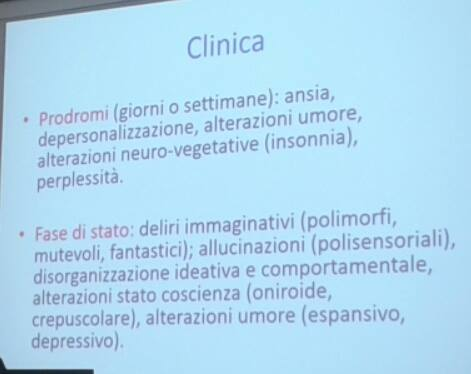
\includegraphics[width=0.9\textwidth]{09/image1.jpeg}
\end{figure}

La prognosi è generalmente favorevole, anche nell' evoluzione naturale
di questi disturbi, ossia anche senza trattamento farmacologico: tendono
ad andare incontro a remissione da sole.

Sono quadri molto importanti perché insorgono in modo drammatico
(sintomatologia accentuata) in persone assolutamente normali (inserite
nella società, con interessi e relazioni interpersonali\ldots{}) e
ovviamente il primo quesito che un medico si deve porre è una netta DD
con quadri più impegnativi.

In altri termini, se esercitiamo in guardia medica e vediamo un
paziente, giovane, con un quadro sintomatologico di deliri e
allucinazioni, dobbiamo pensare più a psicosi acute brevi piuttosto che
a un quadro schizofrenico o di psicosi affettiva.

\subsection{Sintomatologia}

Le psicosi acute brevi si caratterizzano per una \textbf{sintomatologia
positiva} (delirante, allucinogena) molto florida, acuta, difficilmente
quindi passano inosservate e spesso sono innescati da eventi stressanti:
si evidenzia quindi un rapporto tra lo stile di vita e l'insorgenza del
quadro psicotico.

\subsection{Incidenza}

Generalmente i pazienti presentano un'età compresa tra i 30 e i 40 anni.

Tali psicosi acute brevi rappresentano il 3\% dei ricoveri psichiatrici.

\subsection{Risoluzione}

La \emph{risoluzione avviene entro 3 mesi dall'esordio}, e può rimanere
un ricordo dell'esperienza delirante (più nello specifico, si è visto
che tanto più alterato è lo stato di coscienza, tanto meno i pazienti
hanno memoria degli episodi psicotici). La risoluzione è spesso brusca,
sebbene non manchino i casi in cui le PAB si risolvono attraverso delle
fluttuazioni sintomatologiche più graduali, e si deve tenere a mente che
la risoluzione delle PAB è spesso una ``\emph{risoluzione a ponte}'',
cioè il paziente va in remissione completa ma può avere delle recidive
(tanti più episodi si hanno, tanto maggiore è la probabilità di averne
di nuovi, e con una maggior frequenza), per cui il decorso è per
definizione remittente, ed 1/3 dei pazienti mantiene l'autonomia
nosografica (cioè continua ad avere attacchi di PAB), mentre nei
restanti 2/3 ``evolvono'' ad altre forme, soprattutto disturbo bipolare
o schizofrenia.
\\\\
I criteri di Langfeld sono molto importanti per valutare e predire se il
paziente andrà verso la schizofrenia o verso altro.

Spesso però non è facile raccogliere l'anamnesi di un paziente non
riuscendo quindi bene ad intuire se il paziente presenta un ridotto
funzionamento pre-morboso: i quadri clinici talvolta possono essere
molto più complessi.

\emph{Se il quadro delirante non si risolve entro 3 mesi è difficile che
si risolva}, e in questo caso è opportuno rivalutare la diagnosi, perché
si tratta probabilmente di schizofrenia..
\\\\
Caso clinico: \emph{ricovero di una ragazza di 19 anni che aveva
apparentemente un buon funzionamento pre-morboso, aveva una rete di
amici e un fidanzato. Fu ricoverata di urgenza per un quadro psicotico
acuto breve caratterizzato da una sintomatologia delirante allucinogena
(con allucinazioni visive soprattutto, a contenuto terrifico), uno stato
di angoscia e un'alterazione dello stato di coscienza. Tale quadro andrà
incontro a risoluzione in 15 giorni (con terapia farmacologica, quindi
non sappiamo se si sarebbe risolta senza). Lei riprese la vita
precedente anche se nel corso dei mesi, pur non presentando sintomi
psicotici, iniziò a perdere piano piano tutte le sue capacità,
diminuendo quindi il suo funzionamento. Nell'arco di 5-6 mesi ebbe un
altro episodio, molto meno florido, che andò anch'esso in remissione,
dopo il quale il suo declino diventò più evidente, tanto è che nell'arco
di 1 anno e mezzo perse gli amici, il fidanzato, non studiò più e non
uscì più di casa. Questo è stato identificato come un quadro
schizofrenico.}

\emph{Se avessimo indagato bene il pre-morboso della ragazza potevamo
notare degli atteggiamenti che ci potevano insospettire (lei viveva in
un ambito molto protetto, con poche amicizie dell'infanzia, viveva in un
paesino sperduto di montagna, il ragazzo era lo stesso da quando aveva
13 anni, l'attività scolastica era incentrata su uno studio giorno e
notte per ottenere i minimi risultati. }
\\\\
\emph{Domanda:} vi è familiarità? Sì. Essa è un aspetto molto importante
da indagare, soprattutto per riuscire ad inquadrare il disturbo che vi
può essere dietro. Se un paziente viene da una famiglia di
schizofrenici, l'episodio di psicosi acuta breve può nascondere un
disturbo schizofrenico alla base.

\subsection{Diagnosi}

Dal punto di vista diagnostico le PAB non sono semplicissime da
riconoscere, nel senso che, se da un lato danno sintomi molto eclatanti,
con pazienti estremamente deliranti, dall'altro è anche vero che tali
quadri sono spesso sovrapponibili a quelli della schizofrenia in fase
produttiva, e la diagnosi di certezza può quindi essere posta solo su di
un piano longitudinale, cioè osservando l'evoluzione della psicosi nel
tempo, e \emph{la diagnosi differenziale è essenziale dal punto di vista
prognostico}, perché le PAB hanno una \textbf{prognosi molto buona}, in
quanto vanno incontro a remissioni completa e non lasciano
compromissioni, mentre per la schizofrenia la prognosi è scarsa, perché
difficilmente si risolve e anche in remissione lascia spesso una marcata
compromissione del funzionamento del soggetto.

\subsection{DD}

Caso clinico: \emph{siamo laureati da due mesi e siamo in servizio come
guardie mediche, soli e lontani dal ps. Ci arriva un paziente di 18 anni
che due ore prima si presenta con un quadro di deliri e allucinazioni,
angosciato, con alterazione di stato di coscienza di tipo confusonirico
(non sa dove si trova\ldots{}). }

\emph{Possiamo fare un \emph{tossicologico} per vedere se alla base non
vi è una patologia psichiatrica ma un quadro di abuso di sostanze, anche
se non è detto che con un tossicologico negativo si possano escludere
questi quadri (esempio la ketamina che non risulta positiva al test).}

\emph{Con un tossicologico negativo, possiamo intraprendere una DD con
disturbi neurologici quali l'epilessia temporale e in tal caso faremo un
\emph{EEG}.}

\emph{Se l'EEG è negativo, possiamo fare anche una \emph{TAC}. Se anche
essa è negativa ci indirizziamo sempre di più verso una patologia
psichiatrica (è una personalità pre-morbosa? Dobbiamo indagare le
alterazioni affettive, lo stato di coscienza, se vi sono stati eventi
stressigeni precedenti\ldots{}).}

L'importante è differenziare le psicosi acute brevi dagli
\textbf{stati dissociativi}, i quali possono presentarsi con alterazioni
di coscienza di tipo crepuscolare. Quello che ci permette tale DD, è la
presenza di una personalità pre-morbosa di tipo dissociativo,
istrionico. La differenziazione purtroppo è molto difficile, viste le
similarità. Molti quadri che noi psichiatri occidentali inquadriamo come
psicosi acute breve, sono influenzati dalla nostra cultura; culture ad
esempio provenienti dall'Africa, rispondono a eventi stressigeni con
quadri dissociativi. 

\subsection{Trattamento}

I pazienti con psicosi acuta breve vengono trattati con antipsicotici.
Possono essere trattati anche con altri farmaci in base al quadro verso
il quale possono revertare negli episodi futuri. Potremmo quindi dare
stabilizzatori dell'umore (per curare un sospetto di quadro bipolare),
antidepressivi (se sospettiamo una depressione psicotica) etc\ldots{}

Non è una costante che, dopo un primo episodio di psicosi acuta breve,
se ne ripresentino altri benché più episodi vi sono nell'arco della
vita, più è possibile che ve ne siano altri.

La terapia antipsicotica, infatti, viene effettuata per 1 anno, se vi è
stato un unico episodio; se gli episodi sono stati 2, viene mantenuta
per 5 anni; se gli episodi sono stati 3 o più, la terapia viene
effettuata tutta la vita. Benché i quadri siano autorisolvibili, la
terapia viene effettuata per tutta la vita sia per prevenire la
re-insorgenza del quadro sia poiché non siamo certi che i quadri si
ripresentino nello stesso modo, ma potrebbero presentare quadri più
gravi.

\subsection{Altre forme psicotiche brevi}

I \textbf{disturbi psicotici brevi}, inclusi nel gruppo dei disordini
associati alla schizofrenia, sono suddivisibili in
\textbf{\emph{disturbo psicotico breve propriamente detto}} e
\textbf{\emph{disturbo schizofreniforme}}: il disturbo psicotico breve
p.d. è un quadro che dura meno di un mese, ed ha caratteristiche per il
resto sovrapponibili a quelle delle PAB, mentre il disturbo
schizofreniforme è un disturbo del tutto simile alla schizofrenia, ma
che dura meno di 6 mesi, ha anche sintomi negativi e non è escluso che
recidivi o diventi schizofrenia conclamata.

\section{Disturbi deliranti cronici}

\subsubsection{Definizione}

I disturbi psicotici non affettivi non schizofrenici si dividono in due
grandi gruppi: i disturbi deliranti cronici e le psicosi acute brevi.

Paranoia e parafrenia, nei sistemi nosografici attuali, appartengono ai
disturbi deliranti cronici.

Sono disturbi esclusivamente o prevalentemente caratterizzati dal
sintomo delirio, con tendenza alla cronicizzazione. Il delirio non
scompare e, se non trattato, tende ad ingrandirsi sempre più, con una
tendenza centrifuga.

Caso clinico: \emph{un delirio persecutorio inizialmente può interessare
la cerchia della famiglia del paziente (padre e madre che perseguitano
il paziente), per poi estendersi al paese in cui vive, poi all'Italia,
poi al mondo}.

Considerando la classificazione riportata sopra, in genere rientrano
tutti tra i deliroidi secondari, in cui il delirio insorge gradualmente
a partire da una personalità premorbosa. Sono degli sviluppi (sviluppo=
esordio subdolo e graduale, nell'arco di mesi o di anni) deliranti di
personalità.

\subsection{Paranoia}

È caratterizzata, in primo luogo, dal fatto che l'unico sintomo presente
è il delirio: non ci sono allucinazioni, disturbi del pensiero,
disorganizzazione ideativa, disturbi dell'umore.

Secondo la definizione di Kraepelin, è una \emph{malattia autonoma (sia
rispetto alla schizofrenia che ai disturbi dell'umore) e specifica,
caratterizzata dall'insidioso (lento, graduale) sviluppo (a partire da
personalità premorbosa) di un sistema delirante permanente e
incrollabile. }

Il delirio, una volta che si instaura, si espande ed arriva a devastare
la vita dell'individuo. Dal punto di vista della struttura, sempre
\textbf{paranoicale}: è un delirio ben sistematizzato ed elaborato. Il
paziente mette a disposizione tutte le sue capacità di memoria, di
intelligenza, cognitive etc\ldots{} per costruire il suo delirio. Non si
hanno altre manifestazioni psicopatologiche, non si ha deterioramento
delle funzioni mentali del paziente,né segni di destrutturazione della
personalità, come invece avviene nella schizofrenia. Insorge a partire
dai 30 anni.

I deliri della paranoia sono deliri con una \textbf{tendenza
centripeta}, e tendono ad evolversi sempre di più, assumendo comunque le
caratteristiche di un delirio lucido, senza allucinazioni, ma con
presenza di nessi logici, socialità integra, cura di sé mantenuta, ma
con un esistenza completamente divorata dal delirio. Citando un autore,
si può sia che si arrivi ad ``\emph{un'esistenza divorata dal
delirio''}: i pazienti finiscono per distruggere la propria vita, perché
tutto ruota attorno al delirio, che rimane l'unica ragione.
L'affettività è integra, la memoria è salda, la coscienza è lucida, non
si hanno disturbi psicosensoriali.

Dal punto di vista formale sono tutti sostenuti da una modalità
\emph{interpretativa}: si tratta di un lavorio continuo, che dura mesi,
basato su interpretazioni di dati della realtà, volti a confermare il
sospetto delirante. Esempio: \emph{paziente con delirio di gelosia, con
la moglie che rientrava a casa due minuti più tardi del solito.}

Per quanto riguarda i contenuti, quelli classici più frequenti sono
deliri:

\begin{itemize}
\item
  \textbf{Erotomanici}: convinzione delirante di essere oggetto di
  interessi amorosi da parte di una persona, generalmente più bella, più
  elevata come rango sociale.

Il decorso naturale, in era pre-farmacologica, si caratterizzava per la
presenza di tre fasi: in un primo momento il/la paziente si convinceva
dell'idea ed era restio ad accondiscendere a questa proposta d'amore per
vari motivi, legati, ad esempio, al matrimonio (oggetto del delirio
cerca il paziente); nella seconda fase questo amore diventava
indissolubile e voluto, ma non riusciva a concretizzarsi per la presenza
di altre persone che lo osteggiavano (oggetto si unirebbe al paziente,
ma vi sono ostacoli); nell'ultimo momento il paziente arrivava a
sentirsi sedotto ed abbandonato dall'oggetto d'amore, reo di questo
inganno, e si concludeva con omicidio dell'oggetto/suicidio del
paziente.

Caso clinico: \emph{una paziente di 45 anni ricoverata in TSO con
delirio erotomanico in seconda fase, non seguita prima. Aveva visto
l'oggetto d'amore una volta nella sua vita in una palestra, non ne
conosceva il nome (anzi, lei stessa gliene aveva attribuito uno) e non
gli aveva mai parlato. Tutto il delirio era basato su modalità
interpretative: era convinta che, durante lo sguardo che si erano
scambiati, avesse fatto il gesto di sfilarsi l'anello, facendole una
promessa. Era convinta che tutto il mondo osteggiasse questo amore,
anche i medici che l'avevano ricoverata. Al momento del ricovero aveva
già divorziato, non vedeva più i figli, non lavorava più: era
completamente divorata dal delirio.}

Domanda: \emph{Nel delirio erotomanico il paziente diventa pericoloso
per l'oggetto del delirio solo in fase 3 o anche prima?}

Generalmente il delirio erotomanico non si associa ad episodi di
stalking, per esempio, che invece attinge ad altri elementi
psicopatologici. Il paziente non ha rapporti con l'oggetto d'amore, si
bea di questa relazione esclusiva, si crea un mondo distaccato senza
vedere edandare attivamente a cercare l'oggetto d'amore.

\begin{itemize}
\item
  \textbf{Interpretativo}: Il delirio interpretativo è la modalità
  formale tipica della paranoia, che genera un delirio sistematizzato,
  paranoicale. L'interpretatività ne è, anche se non sempre, ovviamente,
  l'elemento caratteristico. Quindi, delirio interpretativo si può
  intenderepraticamente come sinonimo di paranoia
\item
  \textbf{Di persecuzione}
\item
  \textbf{Di querela}
\item
  \textbf{Di grandezza}
\end{itemize}
\end{itemize}

Nella schizofrenia spesso i deliri sono fantastici e bizzarri
(coinvolgono altri mondi, alieni, servizi segreti\ldots{}), per cui
vengono riconosciuti da chiunque.

Nella paranoia invece, soprattutto nelle fasi iniziali, sono molto
legati alla realtà e possono addirittura avere un seguito, finché non
raggiungono dimensioni esagerate: coinvolgono l'amore, il lavoro, la
promozione, il fatto di sentirsi truffati, ecc\ldots{} In passato,
persone con paranoia hanno infiammato le folle, sono riuscite a creare
gruppi e sette, proprio perché inizialmente sono verosimili. Inoltre,
avendo i pazienti una personalità premorbosa, senza destrutturazione
della personalità, sono credibili e per molto tempo riescono a mantenere
una vita sociale normale. Per questo giungono tardivamente
all'osservazione del medico: il problema è che più tardivamente vi
arrivano ed iniziano la terapia farmacologica, più è difficile che il
delirio receda, poiché la cronicizzazione è insita in questi disturbi.
Devono essere colti e trattati tempestivamente, perché altrimenti non
possono essere sradicati: nell'arco del tempo cambiano l'intero assetto
cognitivo del paziente e la sua vita psichica, in funzione del delirio,
che diventa la ragione centrale senza possibilità di toglierlo.

Caso clinico: \emph{una persona che tutti i giorni stava in piazza
davanti ad una banca nelle ore di punta, sopra a delle pertiche, con un
megafono, urlando le nefandezze che la banca gli aveva causato} delirio
di persecuzione e ``querulomane''. Era chiaramente una paranoia, però
inizialmente poteva mostrare credibilità.

Per fare diagnosi di paranoia, \emph{il delirio deve essere presente da
almeno un mese}, e si deve sempre ricordare che la paranoia \emph{emerge
sempre da una \textbf{personalità premorbosa}} (spesso si tratta di
persone rigide, con DP narcisistico, personalità sospettosa o
diffidente). L'esordio della paranoia è \emph{tra i 30 ed i 40 anni},
quindi più tardivo che nella schizofrenia.

I tratti di personalità premorbosa che predispongono alla paranoia
possono essere diversi, non c'è un unico tipo di disturbo.

Un esempio classico è il disturbo paranoide di personalità: chi per
natura è diffidente, sospettoso, è più facile che tenda a sviluppare una
paranoia.

Oppure, tratti narcisistici di personalità: caso clinico: \emph{un
paziente che da anni aspetta una promozione in ambito lavorativo, con
tratti narcisistici che lo sostengono, può sviluppare un delirio
persecutorio in seguito ad un evento trigger, come il conferimento della
stessa promozione ad un collega. }

Vi è sempre un'interazione tra una personalità premorbosa ed uno o più
eventi di vita, a volte insignificanti, ma che vanno a toccare degli
elementi di vulnerabilità del paziente tali da mettere in moto il
delirio. Gli eventi sono diversi, a seconda della natura della
personalità che vi è dietro, e vanno a creare dei nuclei nascosti
affettivi, di vergogna, di insoddisfazione, di insicurezza, che vengono
celati e coperti dal delirio. Esso diventa la `reazione granulomatosa'
che copre il `corpo estraneo', rappresentato dal nucleo affettivo.

Caso clinico: \emph{Il paziente di prima, che riceve la ferita
narcisistica, manifesta questo vissuto di vergogna ed inadeguatezza che
copre col delirio.}

Si vedono in maniera evidente inoltre nelle personalità
insicuro-sensitive (che caratterizzano il \textbf{delirio di rapporto
sensitivo}, descritto per la prima volta da Kretschmer): in queste
persone coesistono sia un elemento di insicurezza, scarsa autostima,
vissuti profondi di inadeguatezza, che elementi sensitivi, stenici,
narcisisti. Sono elementi contropolari che possono favorire il delirio.
L'elemento di vergogna viene nascosto dall'elemento stenico, che è
quello che fa strutturare il delirio.

Esempio, \emph{delirio dei masturbatori: fu un esempio dello stesso
Kretschmer. Bisogna considerare la Germania di inizio Novecento e la
colpa che poteva essere correlata alla masturbazione. I ragazzini,
associati a questo vissuto profondo di vergogna, iniziavano a delirare
uscendo di casa e accorgendosi dello sguardo e dello scherno degli altri
per quello che avevano fatto.}

Ne esistono anche delle forme particolari, come la ``\textbf{follia a
due}'', che si ha quando due o più persone delirano e si influenzano a
vicenda nel delirio: in questo caso abbiamo una personalità più forte,
che idealizza ed induce il delirio, ed una personalità più debole, che
invece ``accoglie'' il delirio.


\subsection{Parafrenia}

È la seconda forma di disturbo delirante cronico e ha una struttura
\textbf{parafrenica}, non paranoica. È un delirio cronico, ma non è
verosimile, né calato nella realtà quotidiana: ha caratteristiche di
contenuto simil-schizofrenico (immaginifico, fantastico, megalomanico,
cosmico).

È sostenuto ed alimentato da fenomeni psicosensoriali-allucinatori
floridi, generalmente polisensoriali: uditivi, visivi, olfattivi,
gustativi. L'età di insorgenza è uguale a quella della paranoia, quindi
età media o pre-senile, più tardiva rispetto all'età della schizofrenia
(16-25 anni, al massimo fino ai 30 anni).

Anche qui non vi è destrutturazione della personalità e non si ha
perdita dello stato di coscienza.

Si ha inoltre \emph{integrità del rapporto con la realtà} (doppio
binario): sono deliri immaginifici che però, a differenza della
schizofrenia, avvengono in pazienti che mantengono una vita
assolutamente normale e irreprensibile ed uno stretto rapporto con la
realtà. Infatti spesso giungono all'osservazione medica per caso,
passano in genere inosservati nonostante delirino per anni e possono
continuare per lungo tempo, a differenza dei paranoici.

Esempio: \emph{donna di 30 anni parafrenica, medico, che fino al giorno
prima del ricovero aveva operato. Aveva deliri misti persecutori,
erotomanici e mistici, immaginava angeli e inglobava persone della vita
reale. }

Domanda: \emph{Come fa un parafrenico ad essere scoperto?}

In quest'ultimo esempio,\emph{il marito scoprì che teneva decine di
diari in un ripostiglio in cui annotava tutto il suo mondo delirante,
scritti per anni (aveva una graforrea).} Quindi, sostanzialmente,
vengono scoperti casualmente.

Domanda: \emph{riguardo alla paranoia e alla parafrenia, abbiamo detto
che insorgono su una personalità pre-morbosa, questa personalità viene
mantenuta?}

La personalità non viene annullata dal disturbo ma è come se tratti già
preesistenti nella personalità diventassero ipertrofici; c'è una
transizione graduale dalla personalità al delirio vero e proprio senza
destrutturazione come nella schizofrenia.

\section{Disturbi di personalità}

\subsection{Introduzione}

\emph{``E' peggio essere malati nell'anima che nel corpo, perché i
malati nel corpo soffrono e basta, i malati nell'anima oltre a soffrire
edificano il loro male.''}

Plutarco

Tutte le patologie psichiatriche (disturbi psicotici, d'ansia,
dell'umore, ecc.) assomigliano molto a delle patologie mediche: ad una
persona capita di ammalarsi di disturbo d'ansia, ad un'altra capita di
ammalarsi di schizofrenia. L'individuo esperisce dei sintomi e la lotta
contro la patologia è la lotta di questo individuo per la salute.

I disturbi di personalità sono molto diversi, si possono descrivere come
la quintessenza dei disturbi dell'anima. Questi malati oltre a soffrire,
citando Plutarco, edificano il loro male. È un disturbo tragico.

\subsubsection{Personalità}

Per parlare di disturbo di personalità, occorre definire una personalità
normale, priva di un quadro patologico.

In condizioni normali secondo l'\textbf{\emph{organizzazione di
personalità}} di Kernberg, la personalità si caratterizza per:

\begin{itemize}
\item
  L'\textbf{Identità}, ovvero il \emph{senso di sé e della propria
  struttura interna}, che consente al paziente di organizzarsi, di
  pianificare, avere delle proprie risorse, dei valori e degli obiettivi
  di vita, sapendo anche come raggiungerli. Nelle forme patologiche di
  personalità, il senso di sé e degli altri appare frammentario, a volte
  estremo, altre volte instabile e superficiale, con marcata difficoltà
  nel comprendere gli altri e nel rispondere in modo adeguato, per cui
  nel paziente si può sviluppare un senso di vuoto, una disforia cronica
  con assenza di investimenti.
\item
  Il \textbf{Livello Predominante dei Meccanismi di Difesa}, cioè
  \emph{i modi di affrontare gli eventi stressanti sia esterni che
  interni}, per cui sono dei meccanismi adattativi, che ci permettono di
  andare avanti e di non suicidarci. Le risposte adattative possono in
  questo caso essere \textbf{\emph{mature}} (sono quelle fisiologiche,
  flessibili in base alla situazione, che ci consentono di interpretare
  la situazione stressante in maniera appropriata e reagire
  opportunamente per controllare lo stress senza distorcere la realtà
  interna o esterna), \textbf{\emph{nevrotiche}} (basate sulla
  \emph{rimozione}, cioè sul bandire dalla consapevolezza l'evento
  stressante, a notevole discapito della flessibilità della risposta,
  che spesso risulta quindi inadatta) o \textbf{\emph{primitive}}
  (basate sulla \emph{scissione}, cioè la compartimentazione delle
  condizioni spiacevoli, le quali risultano ``isolate'' le une dalle
  altre ed emergono in maniera alternata, mai assieme, dando una
  notevole instabilità tra le esperienze contradditorie).
\item
  L'\textbf{Esame della Realtà}, cioè la \emph{capacità di leggere ed
  interpretare i segnali sociali}, rispondendo in modo adeguato ai
  contatti interpersonali, e che viene meno nelle fasi più gravi dei
  disturbi di personalità, in genere in maniera del tutto inconsapevole
  per il soggetto, sebbene vada ricordato che \emph{una prolungata
  perdita dell'esame di realtà non è una caratteristica tipica dei
  disturbi di personalità}, sebbene nelle forme più gravi si possano
  comunque avere alterazioni transitorie, specie se legate a situazioni
  stressanti o all'uso di sostanze.
\item
  La \textbf{Qualità delle Relazioni Oggettuali}, cioè le relazioni
  interpersonali, che in una personalità normale si manifesta come la
  \emph{capacità di comprendere e tenere ai bisogni degli altri
  indipendentemente dai propri}, mentre nei disturbi di personalità
  predomina una visione delle relazioni improntata al soddisfacimento
  dei propri bisogni.
\end{itemize}

A queste quattro caratteristiche di base va poi aggiunta un ulteriore
elemento, che è il \textbf{funzionamento} \textbf{morale}, che
\emph{mette in relazione i valori ed i bisogni dell'individuo con quelli
della società} in cui il soggetto si trova a vivere: in condizioni
normali si ha una dedizione a valori ed ideali che si mantiene coerente
ma tuttavia flessibile, cioè sempre in relazione col senso di sé, mentre
nelle forme patologiche la flessibilità e l'integrazione nel sé viene
meno, ed il funzionamento morale può andare perso (come avviene ad
esempio nel DP antisociale) o risultare eccessivamente rigido ed
intransigente (come nei DP di Cluster C).

\begin{figure}[!ht]
\centering
	\includegraphics[width=0.9\textwidth]{011/image1.png}
\end{figure}

Le
alterazioni dell'organizzazione della personalità sono quindi alla base
di tutte le varie forme di disturbo di personalità, ma bisogna tenere a
mente che la forma specifica di disturbo dipende dai
\textbf{\emph{tratti di personalità}} del soggetto, dove per tratti di
personalità si intendono dei \emph{modelli coerenti di comportamento,
emozioni e di stile cognitivo che dettano le differenze interindividuali
nel comportamento, rimanendo in genere stabili nel tempo o nei
contesti}. La differenza in tratti di personalità determina come noi ci
comportiamo in modo diverso l'uno all'altro, determina quindi la nostra
unicità.

Ad esempio, l'interesse potrebbe essere \emph{``mi piacciono le
feste'',} il valore \emph{``divertirmi}'', le preferenze
\emph{``incontrare gente nuova''}, il comportamento \emph{``vado
volentieri alle feste''}. Questo è un esempio di tratto di personalità.

Per questo motivo ci comportiamo in modo coerente, tant'è che è facile
anche per ciascuno di noi conoscendo i propri amici, prevedere il loro
comportamento. Se per esempio volessimo andare al cinema, sapremmo quale
amico sarebbe più disposto a venire. \emph{\emph{Questo ragionamento è
possibile perché conosciamo quali sono i suoi valori, i suoi interessi,
le sue preferenze e quindi ci è possibile prevedere il suo
comportamento. I tratti di personalità sono quelli che ci rendono
prevedibili e ci aiutano a stare insieme. }}

Ovviamente in tratti di personalità sono del tutto egosintonici, non
vengono avvertiti come problematici (nemmeno quando sono molto deviati
rispetto alla norma!) e a loro volta derivano da un'amalgama tra il
\textbf{\emph{temperamento}} (fattori genetici ereditabili che
influenzano la risposta all'ambiente) e l'\textbf{\emph{esperienza}},
cioè ciò che viene appreso nell'interazione con l'ambiente.

Il temperamento, più nello specifico, è la parte genetica dei tratti di
personalità. \textbf{È la tendenza innata a reagire ai vari stimoli
ambientali}. Innata non vuol dire non modificabile, però quando
nasciamo, già per il fatto di essere nati, abbiamo la nostra piccola,
unica disposizione (che già allora ci rende diversi e unici) a reagire
in un certo modo agli stimoli ambientali.

Da piccoli si può vedere relativamente poco, ma per esempio, c'è il
bambino che piange molto e c'è il bambino che si calma subito.

Il \textbf{\emph{temperamento}},ha delle \emph{caratteristiche
biologiche stabili ed ereditabili, geneticamente determinate}, che si
manifestano attraverso 4 \textbf{dimensioni temperamentali}, le quali
sono tra loro indipendenti:

\begin{itemize}
\item[1.]
  \textbf{Ricerca di stimoli forti e nuovi:}, potenzialmente piacevoli e
  gratificanti nell'ambiente. Rappresenta la nostra voglia di esplorare
  e di avere un reward, una gratificazione dagli stimoli dell'ambiente.
  Questa tendenza di chiama \textbf{ricerca della novità,} ed è
  responsabile, se eccessiva, di comportamenti di impulsività
  (\emph{``non mi basta mai''} -\textgreater{} abuso di sostanze) o,
  all'opposto, di comportamenti di eccessivo ritiro (``\emph{non mi
  interessa} `` -\textgreater{} non cerco niente di piacevole). alcuni
  soggetti hanno una forte tendenza alla ricerca di nuove situazioni,
  mentre altri non le ricercano affatto, risultando spesso noiosi agli
  occhi degli altri.
\item[2.]
  \textbf{Affettività negativa o sistema di inibizione comportamentale}.
  Rende conto della tendenza a reagire a stimoli nuovi e potenzialmente
  pericolosi. Esprime ``come vediamo l'ambiente'': è un ambiente denso
  di pericoli o no? Noi tutti variamo in questo. Avere troppa paura,
  quindi vedere troppi stimoli potenzialmente pericolosi nell'ambiente
  può portare a eccessiva inibizione. D'altro canto, avere troppa poca
  paura può dare ugualmente problemi, si rischia infatti di non imparare
  dagli stimoli negativi.
\item[3.]
  \textbf{Capacità di risuonare in base ai rinforzi sociali}: è la
  nostra capacità di legarci agli altri, la capacità di attaccamento.
  Quanto siamo intaccati da quello che gli altri pensano/dicono di noi e
  da quanto ci stanno vicini.\\
  Se pensiamo all'esclusione interpersonale, è studiatissima in
  psicologia sociale perché noi esseri umani siamo esseri sociali, e
  quindi dobbiamo stare insieme, infatti abbiamo un sistema nel cervello
  chiamato \textbf{sistema per il riconoscimento
  dell'ostracismo}\emph{.} Questo sistema si attiva quando il soggetto
  viene isolato da un gruppo di persone e attiva le stesse aree del
  dolore fisico. Quindi essere ostracizzati è dolorosissimo.

È importante soffrire se gli altri ci abbandonano perché è un campanello
d'allarme. Il dolore sociale ci allerta del pericolo dell'esclusione
sociale, ci dice che c'è qualcosa che non sta andando.

Il segnale ha inizio nella corteccia anteriore del cingolo, prosegue poi
verso la corteccia dorsolaterale prefrontale, che fa modificare il
comportamento in un senso teso a fare riaccettare il soggetto agli
altri.\\
Il problema è che anche in questo caso, essendo una dimensione del
temperamento, è meglio non averne né troppo, né troppo poco. Chi ne ha
troppo poco potrebbe ricordare il primo paziente con Cluster A: infatti
predispone a un isolamento sociale, a una mancanza di empatia. D'altra
parte, averne tanto è ugualmente negativo, in gergo psicologico è
definito \emph{sentimentalismo}. Essere troppo sentimentali vuol dire
essere troppo dipendenti dal giudizio altrui, e potrebbe portare a
compiere azioni spiacevoli per noi stessi pur di tenerci legato chi ci
vuole escludere.

Quindi in alcuni casi si può avere un'ipersensibilità al rifiuto, mentre
in altri casi si ha una totale indifferenza alle lodi o al biasimo degli
altri.

\item[4.]
  Mentre le prime tre dimensioni sono abbastanza automatiche poiché
  conseguono a uno stimolo, la quarta dimensione, chiamata
  \textbf{capacità di autoregolazione}, serve per regolare tutte queste
  tendenze, serve per dire, per esempio: \emph{``Ho un obiettivo:
  quindi, anche se volessi usare cocaina tutti i giorni perché sono un
  impulsivo, questo interferirebbe col mio obiettivo, che è fare
  medicina''.}
\end{itemize}

\begin{figure}[!ht]
\centering
	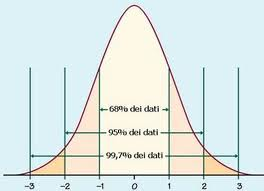
\includegraphics[width=0.9\textwidth]{011/image2.png}
\end{figure}

Ogni
tratto temperamentale si distribuisce normalmente nella popolazione
generale, quindi tutti abbiamo tutti i tratti. La maggioranza delle
osservazioni saranno quindi nell'area centrale o appena laterale. La
maggior parte della popolazione avrà punteggi intermedi, che non
dovrebbero dare grossi problemi. Quando i tratti temperamentali sono
estremi, quindi o troppo alti o troppo bassi, ecco che si costruiscono
anche le prime basi dei problemi.

Il temperamento non è tutta la personalità. Si dice che, a partire dai
tratti temperamentali, io nasco, faccio le mie cose, in parte
selezionate dai miei tratti temperamentali, perché se io sono molto
pauroso tenderò a fare le cose con più cautela.

Le nostre esperienze ed anche un certo apprendimento forgiano i tratti
temperamentali fino a costituire la personalità a tutto tondo.

La personalità si articola in più parti, che riguardano tutte le
modalità di comportamento apprese a partire dai tratti temperamentali e
dalle esperienze di vita. È il modo in cui vediamo il mondo e ci
rapportiamo ad esso. Dunque la definizione di personalità è operativa:
cosa faccio, cosa voglio, quello che si vede fuori di me\ldots{}ecc.

\subsection{Definizione}

Quando si fa il salto PERSONALITA' NORMALE DISTURBO DI PERSONALITA'?

Se i tratti di personalità diventano rigidi, intensi, si amplificano e
perdono flessibilità, si parla di disturbi di personalità.

Disturbo di personalità: \textbf{Fallimento che coinvolge 3 aree di
funzionamento dell'individuo, distinte, ma tra loro collegate:
\emph{sistema del Sé}, \emph{relazioni familiari o di parentela},
\emph{relazioni sociali o di gruppo}.}

\begin{itemize}
\item
  \emph{\textbf{Sistema del Sé}}: è l'idea che io ho di me, quello che
  voglio da me e dalla vita, i miei obiettivi e i miei valori.
\item
  \emph{\textbf{Relazioni familiari}}: come sto con i miei familiari,
  che possono essere: padre, madre, marito/moglie, figli.
\item
  \emph{\textbf{Relazioni sociali}}.
\end{itemize}

Cosa c'è nella vita di una persona, oltre a questi tre ambiti, che non
viene intaccato?

Nella vita di una persona normale non avanza nulla, non esista niente al
di fuori di queste tre aree.

\textbf{Il disturbo di personalità è un fallimento dell'individuo nella
sua interezza.}

Chiaramente questa è una definizione, non significa che tutti i soggetti
affetti da DP sono ugualmente deteriorati in tutte queste aree.

Secondo la definizione del OMS, il disturbo di personalità è un
\textbf{\emph{grave disturbo nel carattere e nelle tendenze
comportamentali dell'individuo, che in genere coinvolge diverse aree
della personalità ed è pressoché invariabilmente associato a gravi
deficit personali o sociali}}. Secondo la definizione di Livesley del
1998, inoltre, il disturbo di personalità può essere visto come ``
\emph{un fallimento che coinvolge tre aree funzionali dell'individuo,
distinte ma correlate: il sistema del Sé, le relazioni familiari e di
parentela e le relazioni sociali o di gruppo}''.

Per meglio definire le caratteristiche di questi disturbi si ricorre ai
criteri del DSM-IV TR, che devono essere presenti per poter porre
diagnosi corretta di disturbo di personalità:

\begin{itemize}
\item[1.]
  Dev'essere presente un \textbf{modello abituale di esperienza
  interiore e di comportamento che devia marcatamente rispetto alle
  aspettative culturali dell'individuo}, manifestandosi in 2 o più delle
  seguenti aree:
  \begin{itemize}
\item
  \textbf{\emph{Cognitività}} (cioè il modo di percepire ed interpretare
  se stessi, gli altri e gli avvenimenti che ci circondano); Sono cose
  che noi facciamo in automatico. Nei pazienti con DP qui c'è una
  distorsione: percepiscono se stessi, gli altri e gli avvenimenti in
  modo distorto.
\item
  \textbf{\emph{Affettività}} (cioè la varietà, l'intensità e
  l'adeguatezza della risposta emotiva); :.
\item
  \textbf{\emph{Funzionamento Interpersonale}}; ovvero realtà esterna,
  come io funziono con gli altri
\item
  \textbf{\emph{Controllo degli Impulsi}}. comportamento + realtà
  esterna.
\end{itemize}
\item[2.]
  Tale modello abituale risulta \textbf{inflessibile e pervasivo} in
  un'ampia varietà di situazioni personali e sociali. Avere una
  difficoltà nel controllo degli impulsi (non è il singolo impeto d'ira
  che porta a fare magri un gesto sconsiderato). È un comportamento
  ricorrente.
\item[3.]
  Il modello abituale determINa un \textbf{disagio clinicamente
  significativo e compromissione del funzionamento} sociale, lavorativo
  e di altre aree inportanti.
\item[4.]
  Il modello si presenta \textbf{stabile e di lunga durata}, e l'esordio
  può essere fatto risalire almeno all'adolescenza o alla prima età
  adulta. Non si fa formalmente diagnosi prima dei 18-20 anni perché la
  personalità è ancora in evoluzione per tutta l'adolescenza e
  probabilmente per prima parte dell'età adulta, però in realtà
  clinicamente gli antecedenti dei DP dell'età adulta si vedono anche
  negli adolescenti.
\item[5.]
  Il modello abituale \textbf{non risulta meglio giustificato da una
  pregressa malattia psichiatrica o dall'assunzione di sostanze} ad
  azione psicotropa.
\end{itemize}

Da questi criteri si può quindi concludere che i pazienti con disturbo
di personalità sono soggetti che si caratterizzano per
un'\textbf{\emph{incapacità stabile e pervasiva di amare e di
lavorare}}.

\emph{Amare} è da intendere in senso lato: avere relazioni reciproche
soddisfacenti (anche di amicizia o buona colleganza).

\emph{Lavorare} significa avere un obiettivo, applicarsi per
quell'obiettivo e farlo funzionare nella vita di tutti i giorni.

Per adottare una vecchia definizione di Schneider, si può dire che i
pazienti con disturbi della personalità sono ``\emph{pazienti che, per
il loro modo di essere fatti, soffrono o fanno soffrire gli altri}''.

\subsection{Diagnosi}

\begin{figure}[!ht]
\centering
	\includegraphics[width=0.9\textwidth]{011/image3.png}
\end{figure}

Questi
sono gli elementi da valutare per la diagnosi generale di DP. Se non c'è
un disfunzionamento in queste 4 aree, non c'è un disturbo di
personalità.

\begin{itemize}
\item
  \emph{Disfunzionamento nel sé:}
\begin{itemize}
\item[1.]
  \emph{Concetto di identità}: esperienza di me stesso come unico,
  chiari confini tra sé e gli altri, stabilità dell'autostima,
  accuratezza della valutazione di sé, capacità di regolare un intero
  range di esperienza emotiva.
\item[2.]
  \emph{Autodirezionalità}: capacità di cercare e perseguire obiettivi
  di vita coerenti e con significato sia a lungo che a breve termine,
  valori morali e di senso etico.
\end{itemize}
\item
  \emph{Disfunzionamento delle realtà interpersonali}
\begin{itemize}
\item[1.]
  \emph{Disfunzione nell'empatia}: persone che in vario modo non
  riescono a comprendere ed apprezzare le motivazioni degli altri e a
  capire l`effetto del proprio comportamento sugli altri.
\item[2.]
  \emph{Disturbo dell'intimità.}
\end{itemize}
\end{itemize}

\subsection{Epidemiologia e sfide dei DP}

I disturbi di personalità sono patologie psichiatriche relativamente
comuni nella popolazione generale, in cui si stima abbiano una
\emph{prevalenza del 10-15\%}, e purtroppo sono disturbi che tendono
frequentemente ad associarsi ad altre condizioni psichiatriche, di cui
complicano la diagnosi, il decorso e soprattutto la terapia: tra queste
vanno ricordate l'abuso di alcol e sostanze, nonché gli episodi
depressivi ed i disturbi d'ansia, ma non bisogna dimenticare che questi
pazienti avranno comunque difficoltà relazionali, problemi abitativi e
disoccupazione frequente, ed hanno un maggior rischio di morte per
suicidio o per altre cause. All'interno dei pattern psichiatrici,
inoltre, come già accennato, la prevalenza di questi disturbi tende ad
essere molto più elevata, arrivando a soglie anche del 50-70\%, proprio
perché raramente questi disturbi si presentano in forma isolata.

Per definizione, il paziente con disturbo di personalità è ``\emph{il
paziente che non piace agli psichiatri}'', per il semplice fatto che
quando giungono all'attenzione medica (spesso costretti dagli altri, in
quanto loro si ritengono generalmente normali) hanno una
\emph{presentazione clinica urgente e caotica}, sono difficilmente
trattabili, e presentano una \emph{combinazione di diversi quadri}, che
vanno dall'autolesionismo all'abuso di sostanze e a problemi
interpersonali di tutti i tipi. Inoltre, ciò che risulta veramente
complesso con questi pazienti è la \emph{terapia}, poiché sono soggetti
con una \emph{bassissima compliance}, e tendono ad abbandonare il
trattamento anche in pochi giorni (il cosiddetto fenomeno delle
``\emph{revolving doors}''), salvo ripresentarsi dopo poco tempo al
pronto soccorso per fenomeni di autolesionismo o attacchi d'ansia. Per
tali motivi, i pazienti con disturbi di personalità \emph{inducono un
senso di inadeguatezza ed incertezza nello psichiatra}, poiché non sono
per niente facili da gestire e sono del tutto restii ad instaurare
un'alleanza terapeutica col medico.

\subsection{Classificazione dei disturbi di personalità}

I disturbi di personalità vengono tipicamente suddivisi in tre gruppi
principali, detti ``\textbf{\emph{clusters}}'', indicati con le lettere
dell'alfabeto \textbf{A}, \textbf{B} e \textbf{C}.

Questo significa che comunque questi pazienti vedono soddisfatti tutti
quei criteri generali di cui abbiamo parlato finora, ma cambia per ogni
gruppo il modo in cui queste difficoltà vengono manifestate.

\begin{table}
%\caption{Please write your table caption here}
\begin{tabular}{p{0.3\textwidth}p{0.3\textwidth}p{0.3\textwidth}}
\hline\noalign{\smallskip}
\textbf{\emph{Cluster A}} & \textbf{\emph{Cluster B}} & \textbf{\emph{Cluster C}}  \\
\noalign{\smallskip}\svhline\noalign{\smallskip}

DP Schizotipico &	DP Antisociale	& DP Evitante \\
DP Schizoide &	DP Narcisistico & DP Dipendente \\
DP Paranoide &	DP Istrionico &	DP Ossessivo-Compulsivo \\
 & DP Borderline & \\

\noalign{\smallskip}\hline\noalign{\smallskip}
\end{tabular}
\end{table}


\subsubsection{Cluster A: ``eccentrico''}

Il paziente del cluster A i caratterizza per la presenza di pensieri e
comportamenti bizzarri o inusuali, e anche per un'incapacità o
disinteresse nello stabilire relazioni soddisfacenti.

Riferendoci ai criteri generali, possiamo affermare che questi pazienti
hanno difficoltà nella cognitività (mondo interno): i pensieri sono
bizzarri e inusuali. A livello interpersonale (mondo esterno) hanno un
disinteresse a stabilire relazioni soddisfacenti.

\emph{Caso clinico: Paziente maschio, inviato dal medico di medicina
generale (MMG) ai servizi, dopo la morte del padre con cui viveva.}

\emph{Il MMG nel raccontare il caso ai colleghi dei servizi psichiatrici
racconta quello che sa della famiglia e quello che il pz nel corso del
tempo gli ha detto:}

\emph{Il pz descriveva il padre come distante, e in anamnesi aveva avuto
un `esaurimento nervoso' in gioventù e, secondo il paziente, il padre
`sentiva le voci' {[}probabilmente aveva un disturbo dello spettro
schizofrenico{]}. Spesso il pz quando andava a trovare il medico curante
si lamentava con lui di come il SSN avesse `abbandonato' il padre, ma
negava di avere egli stesso problemi di salute. Era però da sempre
affascinato dall'occultismo, e pensava continuamente all'eutanasia,
specie dopo la morte del padre.}

\emph{Anamnesi fisiologica: Era stato un bambino timido e un adolescente
solitario, senza mai aver avuto contatti al di fuori del nucleo
familiare. Aveva lavorato solo a tratti, per brevi periodi e in
situazioni solitarie, cioè lavori in cui non ci fossero colleghi (es
magazziniere). Era stato coinvolto in qualche `zuffa' in strada, ma non
aveva mai riportato condanne. Non aveva mai avuto esperienze sessuali né
sentimentali. Ora viveva solo con la madre anziana.}

Analizzando la breve storia in base ai criteri generali rileviamo:

\begin{itemize}
\item
  Mondo interno: uniche preoccupazioni sono cose un po' bizzarre
  (pensare solo all'eutanasia) -\textgreater{} alterazioni nella
  cognitività.\\
  zuffe in strada -\textgreater{} difficoltà nel controllo degli impulsi
\item
  Realtà esterna: mai avuto rapporti di amicizia/ sentimentali
  -\textgreater{} deficit nelle relazioni interpersonali.
\end{itemize}

\emph{Ai colloqui psichiatrico si presenta scarsamente accessibile (non
parla), appare assorto nei propri pensieri; trova difficile rispondere
alle domande dello psichiatra, anche alle più banali. Risponde quasi a
monosillabi e in modo molto minimizzante. Tuttavia non vi sono segni di
disturbo dell'umore o psicosi. La madre riferisce che il pz come sua
unica attività (pz disoccupato) passa il tempo su internet, a fare
ricerche sull'eutanasia, e che ciò `non è sano'.}

Questo è un esempio di disturbo schizotipico di personalità. Può
preludere alla schizofrenia, tra tutti i disturbi è un po' diverso,
perché fa parte del cosiddetto spettro schizofrenico, costituisce la
vulnerabilità genetica alla schizofrenia: infatti è più frequente nei
familiari di I grado di pazienti con schizofrenia, e viceversa. Non ci
sono franchi deliri, non ci sono franche allucinazioni, ma c'è comunque
il distacco dagli altri.

\emph{In questo caso è necessaria una valutazione delle abilità sociali
e lavorative (dal momento che è incline a scoppi di rabbia, se gli viene
richiesto di essere più socievole) e del rischio per sé ed altri (es: vs
la madre, per via dei pensieri circa la eutanasia).}

\subsubsection{Cluster B: ``drammatico''}

Sono fra i pazienti più difficili per gli psichiatri, \emph{``the
patients psychiatrists dislike''.}

Si caratterizzano per la presenza di comportamenti impulsivi, teatrali,
esagerati e instabili. L'instabilità è la quintessenza di questi
disturbi, riguarda sia mondo esterno che mondo interno.

Caso clinico: \emph{Ragazza di 22 anni, già nota ai servizi
psichiatrici; disoccupata. Ricoverata in servizio psichiatrico di
diagnosi e cura (SPDC) un sabato notte (in urgenza), dopo accesso al PS
per essersi tagliata i polsi a seguito di una lite con l'ex fidanzato.
Questa è solo l'ultima di una serie di relazioni violente con gli
uomini, tutte durate non più di alcuni mesi. La pz è già rimasta incinta
5 volte, ma solo 2 gravidanze erano andate a termine, e i 2 i figli
erano stati entrambi affidati ai servizi sociali alla nascita.}

\emph{\\
}Analizzando la situazione in base ai criteri generali dei DP si
riconosce facilmente il disfunzionamento interpersonale. La definizione
generale dice: ``incapacità di amare e lavorare'', non ci dice come. Nel
pz di prima c'era disinteresse e distacco, in questo invece sembra
esserci ipercoinvolgimento.

Emerge altresì il quadro tipico di inflessibilità e pervasività del
disturbo. Non si può dire che la pz sia stata sfortunata: ha trovato un
uomo violento e poi si è messa con uno bravo, ha continuato ad avere
relazioni violente con gli uomini. Allo stesso modo il pz del caso
precedente non si era isolato in un periodo della sua vita, era sempre
stato isolato\emph{. Il pattern è inflessibile, pervasivo in una varietà
di contesti sociali e interpersonali.}

Da ricordare anche come nella popolazione generale questi soggetti
vadano incontro a tutta una serie di problemi (disoccupazione, problemi
relazionali, ecc.), nella fattispecie l'allontanamento, appena dopo la
nascita, dei due figli.

\emph{La pz è figlia di una relazione di breve durata tra il padre e la
madre, che in seguito ebbe molti partners, qualcuno dei quali abusava
sessualmente della pz. Descritta come intelligente alle elementari,
inizia però presto a marinare la scuola e già alle medie viene sospesa
per aggressività sia verbale che fisica verso un insegnante e per uso di
droghe `leggere'. Dopo aver lasciato la scuola (alle medie), inizia ad
usare eroina e a prostituirsi per procurarsela. }

Da notare il disfunzionamento interpersonale che si manifesta con
l'aggressività. È chiaro inoltre che il compito di una bambina di 12
anni dovrebbe essere quello di andare a scuola, avere degli amici e
crescere, non di marinare la scuola, farsi sospendere e usare droghe
``leggere''. \emph{Il modello quindi devia rispetto alle aspettative
della cultura dell'individuo, c'è un fallimento nelle aree del sé.}

Ad un'analisi più attenta si notano delle similitudini tra la storia
della pz e quella della madre. Non è un evento casuale, sicuramente
hanno un ruolo la base genetica e un ``apprendimento'' del vissuto
materno. L'abuso sessuale costituisce poi un'aggravante ulteriore in
questa storia, soprattutto considerando il tipo di uomini ugualmente
violenti che poi ricerca la pz. La devianza si nota dal fatto che a
seguito di un'esperienza negativa si perpetui la ricerca di relazioni
abusanti con gli uomini.

Plutarco diceva che sono persone che edificano il loro male: c'è
qualcosa in lei che le impedisce di prendersi ciò che di buono c'è al
mondo.

\emph{All'EO presenta cicatrici multiple su braccia e addome. Spiega
allo psichiatra che si sente `vuota' e `morta dentro', e che questi
sentimenti vengono alleviati, almeno nel breve termine, dal ricorso
all'autolesionismo. Talora riferisce di sentire una `voce maschile'
dentro di lei, in assenza di segni di franca depressione o psicosi. }

\emph{Spesso nei pazienti con disturbi del cluster B ritroviamo
autolesionismo}: si tagliano, si spengono sigarette addosso.

Le motivazioni addotte per giustificare il comportamento possono essere
del tipo:

\emph{``C'era una tensione intollerabile, ma era una tensione interiore,
preferisco sentire il dolore fisico, almeno lo posso codificare,
altrimenti io non so che cosa ho dentro''}

\emph{``Se lei si sentisse che non esiste, non vorrebbe almeno avere la
sensazione di esistere un attimo?''.}

E' importante sottolineare come il sentire una voce maschile in questo
caso non costituisca un'allucinazione, in quanto il paziente
schizofrenico ha in più un giudizio di realtà del tipo\emph{: ``mi hanno
detto che''}. In questi pazienti invece è definito un sintomo quasi
psicotico, dicono \emph{``mi sembra di avere una voc}e'', come se fosse
la coscienza sonorizzata.

\emph{In reparto si adatta rapidamente alla routine della degenza e non
dà segni di essere depressa. Stringe amicizia con i pazienti più
giovani, e chiede continuamente favori ai membri più giovani dello
staff, divenendo talora invadente, e sessualmente inappropriata. Dopo 3
giorni si allontana dal reparto e rientra con delle canne, che offre ai
codegenti. Viene dimessa una volta scoperto tale comportamento, dal
momento che non vi erano gli estremi per TSO, con l'indicazione a
valutazione e presa in carico psicoterapica ambulatoriale.}

Ricapitolando: la paziente è arrivata un sabato notte, disperata, si
sente morta dentro, lite con l'ex, si è tagliata i polsi. Ci sarebbe da
aspettarsi una persona depressa nei giorni successivi, invece si adatta
brillantemente.

Ricercando i criteri generali:

\begin{itemize}
\item
  \textbf{Mondo interno}: la sensazione di ``essere vuota e morta
  dentro'' è alterata e fortemente in contrasto con il comportamento dei
  giorni successivi. Discontrollo degli impulsi: si taglia.
\item
  \textbf{Mondo esterno}: il rapporto con gli altri è inadeguato e
  distorto.
\end{itemize}

In pratica si vede una chiara deviazione da quello che ci si
aspetterebbe nella determinata condizione. Se un pz è ricoverato perché
non sta bene, vorrà stare meglio, sa perfettamente come ci si dovrebbe
comportare in un reparto, di certo sa che non può tornare con delle
canne.

\subsubsection{Cluster C: ``ansioso''}

I pazienti del \textbf{\emph{cluster C}}, che hanno \emph{atteggiamenti
inibiti}, sono \emph{molto timidi ed ipersensibili alla
disapprovazione}.

Caso clinico: \emph{Pz femmina, 40 anni ca., madre di 4 figli e di
recente separatasi dal marito dopo 20 anni di matrimonio. Inviata al
consulente psichiatra dal MMG, che la descrive come una donna gentile, a
modo, devota alla famiglia, ma incline a chiedere numerose visite per
vari sintomi fisici. Ora la pz era giunta dal MMG in lacrime, sconvolta
dalla consapevolezza che il marito l'aveva lasciata. La figlia maggiore,
che l'accompagna, riferisce una lunga storia di agorafobia, in
precedenza occultata dalla pz, che se ne vergognava.}

\emph{La pz era figlia unica di genitori anziani. Da sempre aveva
mostrato scarsa stima di sé, con difficoltà a frequentare la scuola,
dove veniva presa in giro come la `cocca' degli insegnanti. Aveva però
un buon rendimento scolastico.}

Le relazioni interpersonali qui sono problematiche in un altro modo
ancora, così come anche la capacità di perseguire i propri obiettivi
(sistema del sé). Questa paziente è studiosa, brava a scuola, però fa
fatica ad avere continuità in questo, perché è disturbata dalla paura
degli altri, è ipersensibile alla disapprovazione.

\emph{Lascia la scuola a 16 anni e sposa un uomo più vecchio, amico di
famiglia, rimanendo subito incinta} {[}non ha altri amici oltre alla
famiglia{]}. \emph{A casa è dedita alla pulizia e all'ordine, e mantiene
delle regole domestiche così rigide che sia il marito sia i figli si
sentono a disagio. Aiuta il marito a tenere i conti della sua attività,
con tale successo che egli (e quindi anche la pz) può andare presto in
pensione. }

\emph{Il cambiamento nella routine ha effetti devastanti sulla pz. Il
marito avrebbe voluto viaggiare `approfittando' della nuova condizione
di libertà, ma la pz rifiuta di seguirl. Il marito inizia una relazione
con una donna più giovane e lascia improvvisamente il tetto coniugale.}

\emph{Viene inviata per valutazione a psicoterapia.}

La paziente non si trova un lavoro fuori da casa, resta a lavorare con
il marito, ed è così dedita alla produttività che gli permette di
raggiungere una sicurezza economica tale da potersi permettere anzitempo
la pensione. A quel punto il marito vorrebbe viaggiare, ma la paziente
non riesce: ha bisogno di lavorare, di tenere sotto controllo l'ambiente
domestico, e in più è agorafobica. \emph{Sono pazienti che tipicamente
nel tempo libero crollano: il tempo destrutturato, quello che non è
dedito alla produttività è fonte di angoscia terribile. }

Questo è un tipico esempio di DP di cluster C con tratti
ossessivo-compulsivi, dipendenti in comorbilità con un disturbo d'ansia
(agorafobia).

\subsection{Eziopatogenesi dei disturbi di personalità}

Come per molti altri disturbi psichiatrici, \emph{l'eziologia dei
disturbi di personalità non è nota}, anche se è ormai chiaro che queste
forme psichiatriche sono il frutto di una complessa interazione tra
fattori ambientali, biologici, psicologici e genetici, come dimostrato
dalla maggior incidenza tra i parenti biologici di primo grado e
dall'elevata, seppur non totale, concordanza tra gemelli omozigoti.

\subsubsection{Modello biopsicosociale}

Per spiegare i disturbi di personalità si usa il modello
BIOPSICOSOCIALE. Non esiste una causa del disturbo, ma diversi fattori
di rischio concorrono a facilitare la transizione da personalità a
disturbo di personalità.

I fattori di rischio sono appunto biologici, psicologici e sociali.

\begin{itemize}
\item[1.]
  BIOLOGICI: varianti estreme del comportamento. Coloro che nascono già
  geneticamente con profili molto intensi di uno dei 4 tratti. Sono
  persone che faranno fatica a regolare il loro temperamento.
\item[2.]
  PSICOLOGICI: nella storia personale dei pazienti, spesso si trova una
  serie di eventi di vita avversi, nell'infanzia o nell'adolescenza.
  Sono persone che spesso riportano una storia di trauma: abuso non solo
  sessuale, ma anche fisico; indifferenza genitoriale ecc. Questo però
  non è la causa del disturbo di personalità. Non può da sola portare al
  disturbo.
\item[3.]
  SOCIALI: anche quando le persone crescono possono avere dei fattori di
  rischio sociali. Si puo' avere \emph{isolamento}, \emph{relazioni
  tempestose con persone abusanti (}ricordare l'esempio della ragazza
  che aveva avuto molte storie e diverse gravidanze e aborti). Tutti
  questi sono eventi di vita maggiori che sarebbero importanti per
  chiunque.
\end{itemize}

Quindi il modello biopsicosociale dice che \textbf{bisogna tener conto
di diversi fattori di rischio che combinandosi insieme possono
predisporre ed eventualmente portare ad un disturbo di personalità.}

\subsubsection{Modello diatesi-stress}

Una variante di questo modello è il modello DIATESI-STRESS, che è un po'
più preciso, ma dice la stessa cosa. La diatesi è la predisposizione a
specifici disturbi di personalità. Di per sè non causa disturbo.

Se ricordiamo i 3 casi clinici della scorsa volta, ci può già venire in
mente qualcosa.

\emph{Caso clinico 1}: \emph{Ad esempio il primo caso: uomo che stava
isolato e pensava all'eutanasia.} Tra i fattori di temperamento citati,
quello particolarmente intenso, maladattativo e problematico in questo
caso è il distacco: il tratto che ci dice se siamo capaci di risuonare
in accordo ai segnali sociali. Lui non riusciva a stare insieme agli
altri. Quest'uomo non era minimamente interessato a ciò che pensavano
gli altri; non aveva reazione né se qualcuno lo isolava, né se lo
lodava.

\emph{Caso clinico 2}:Un altro caso clinico visto è quello della ragazza
che faceva confusione e non stava alle regole. Il tratto problematico
qui poteva essere l'impulsività. Lei aveva bisogno di essere sempre
stimolata.

\emph{Caso Clinico 3:}Il terzo caso clinico invece mostra tra i tratti
di personalità più accentuati l' inibizione, la tendenza ad essere
impauriti da stimoli nuovi. La signora di questo caso aveva questo
problema già da piccola. Lei non riusciva ad andare a scuola. Il suo
problema non era concentrarsi sullo studio, ma allontanarsi dagli altri
perché aveva paura. La ragazza, in più, soffriva di agorafobia: stava
sempre chiusa in casa.

Analizzando singolarmente questi 3 casi, possiamo dire che ciascuno di
loro, oltre ad avere un tratto molto intenso, predominante sugli altri e
poco plastico, ha anche una bassissima capacità di autoregolazione.

I tratti del temperamento rappresentano la predisposizione a specifici
disturbi di personalità. È più probabile che una persona molto impulsiva
possa avere problemi col CLUSTER B ed una persona molto paurosa problemi
riconducibili al CLUSTER C.

Il modello DIATESI-STRESS dunque, dice che, \textbf{a partire da una
predisposizione, a seconda o meno che un soggetto incontri nella vita
fattori stressanti, si determina la soglia oltre la quale i tratti di
personalità diventano maladattativi, causano problemi}.

\emph{Per avere disturbo di personalità, un soggetto deve avere un
fallimento, un disagio \textbf{clinicamente significativo} nel mondo
interno e nella realtà esterna. }

Quindi l'interazione tra la diatesi e lo stress porta ad un disturbo di
personalità o, come diceva Schneider, alla comparsa di persone che, per
come sono fatte, soffrono o fanno soffrire gli altri.

I disturbi di personalità dunque non hanno una causa soltanto, ma più
fattori che interagiscono tra loro.

C'è interazione tra i tratti di personalità genetici, il temperamento e
i fattori stressanti. Non è un mescolamento tra questi due fattori che
crea il disturbo di personalità. Per capire lo strutturarsi di un
disturbo di questo tipo, bisogna capire che la relazione tra essi non è
casuale.

\begin{figure}[!ht]
\centering
	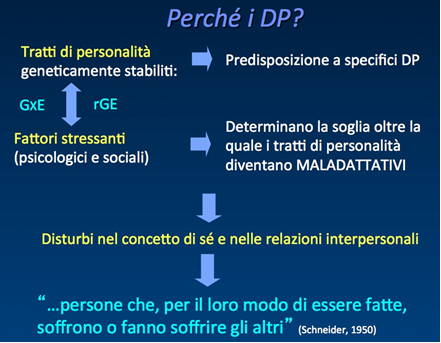
\includegraphics[width=0.9\textwidth]{011/image4.png}
\end{figure}

Il tutto viene spiegato da due semplici sigle GxE e rGxE.

\paragraph{GxE INTERAZIONE GENE-AMBIENTE}

\begin{figure}[!ht]
\centering
	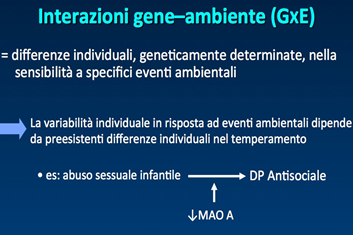
\includegraphics[width=0.9\textwidth]{011/image5.png}
\end{figure}

Non
c'è relazione casuale tra temperamento e ambiente.

Esistono differenze individuali geneticamente modificate nella
sensibilità a specifici eventi ambientali.

Questo spiega bene la questione dell'abuso, del trauma. Per quanto
l'abuso e il trauma siano dei rischi maggiori per qualsiasi disturbo
psichiatrico, non tutte le persone che lo hanno subito sviluppano in età
adulta un disturbo di personalità o psichiatrico di altro tipo.

Questo vuol dire che noi \textbf{reagiamo agli stimoli in modo diverso}.
Tra di noi ci saranno persone più o meno sensibili.

Dunque la variabilità individuale in risposta ad eventi ambientali
dipende da preesistenti differenze individuali nel temperamento.

La ricerca ha dimostrato che gli individui che hanno buone capacità di
autoregolazione, sono quelli più resilienti nei confronti degli eventi
stressanti. Anche se capitano, ho più probabilità di superarli. Tutte le
varianti maladattative delle tre dimensioni conferiscono una maggiore
sensibilità. Importante fu uno studio genetico pubblicato su science che
andò a vedere la relazione tra abuso sessuale infantile e successivo
sviluppo di \textbf{disturbo di personalità antisociale}. E' un disturbo
gravissimo per cui non c'è cura. Queste persone non guariscono e devono
stare in carcere perchè sono delinquenti, serial killer ecc. Nelle serie
americane, quando disegnano il profilo psicologico del serial killer,
mettono sempre che lui, da piccolo, aveva subito abusi, crudeltà; e
questo è vero. Le persone fredde, senza empatia, che godono nel far
soffrire gli altri e non c'è modo di guarirli, hanno avuto una storia di
crudeltà su loro stessi quando erano piccoli.

Rimane il fatto che non tutti quelli che hanno subito degli abusi o
violenze, dopo diventano antisociali. Lo studio infatti ha fatto vedere
che c'è una sorta di verità: C'è correlazione tra abuso e sviluppo di
personalità antisociale solo nei soggetti che hanno bassa attività dell'
enzima MAO A. Questo dunque è un esempio di interazione gene ambiente.

\paragraph{rGxE CORRELAZIONE GENE-AMBIENTE}

\begin{figure}[!ht]
\centering
	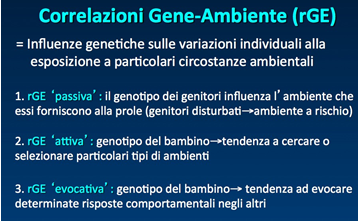
\includegraphics[width=0.9\textwidth]{011/image6.png}
\end{figure}

E'
ben diverso dall'interazione gene ambiente citata prima.

Ci dice che esistono influenze genetiche sulle variazioni individuali
all'esposizione a particolari circostanze ambientali.

Non è semplicemente che io sono diverso da un altro nella mia
sensibilità agli eventi stressanti, ma sono diverso anche per come mi
espongo agli eventi stressanti.

Esistono 3 tipi di correlazione gene-ambiente:

\begin{itemize}
\item[1.]
  \textbf{rGxE ``PASSIVA'':} \emph{Il genotipo dei genitori influenza
  l'ambiente che essi forniscono alla prole.} Pensiamo al 2\^{} caso
  clinico: la madre ha avuto la figlia da giovane. Il padre biologico
  della bambina l'aveva lasciata e da li, la donna ha avuto numerosi
  partner violenti di breve durata e questi abusavano della figlia.
  Quello che noi vediamo è che la ragazza da grande ha un disturbo
  borderline di personalità. Questo è l'effetto del fatto che è
  cresciuta in un ambiente a rischio o è l'effetto del genotipo della
  madre che si è comunque trasmesso a lei? Entrambe le cose. La ragazza
  ha ereditato un genotipo predisponente dalla madre e vivendo in un
  ambiente a rischio ha fatto tracimare le cose. Se ho un genitore
  disturbato è verosimile che io erediti i suoi geni. Però centra anche
  l'ambiente perché i genitori non solo mi hanno passato un genotipo
  predisponente, ma mi hanno tenuta in un ambiente problematico, pieno
  di eventi stressanti. Non è casuale che io abbia una predisposizione
  genetica e mi trovi a vivere in un ambiente già pericoloso per il
  rischio di sviluppare il disturbo di personalità.
\item[2.]
  \textbf{rGxE ``ATTIVA'':} \emph{Il modo in cui io sono fatta
  geneticamente, mi predispone a cercare nel mondo e a selezionare
  alcuni tipi di ambiente.} Sempre l'esempio di prima, fa vedere che la
  ragazza già alle medie marina la scuola, viene espulsa e dunque
  abbandona la scuola stessa. In seguito entra in un gruppo di gente che
  si droga ed inizia a prostituirsi per avere eroina. Le relazioni a
  rischio già nell'adolescenza, come avere amici drogati, sono un grosso
  fattore di rischio per i disturbi di personalità, ma anche in questo
  caso il fatto non è casuale. La ragazza era così impulsiva che gli
  stimoli normali, di una classe delle medie, non le bastavano; doveva
  andarne a cercare altri fuori. \emph{La ragazza, a causa del suo
  temperamento, ha attivamente cercato degli ambienti a rischio.}
\item[3.]
  \textbf{rGxE ``EVOCATIVA'':} \emph{Il genotipo del bambino causa la
  tendenza di evocare certe risposte comportamentali negli altri.} La
  ragazza quando era a scuola, faceva tanta confusione che è stata
  espulsa. Ha perso un fattore protettivo. Andare a scuola vuol dire che
  si è in grado di seguire le tappe evolutive normali di una persona.
  Lei però evocava negli insegnanti o negli amici ``bravi'' una reazione
  di espulsione. Più avanti evoca la reazione di espulsione nei
  partners: prima li cerca e poi si comporta in modo così caotico che
  tutti la lasciano.
\end{itemize}

Prendiamo come altro esempio il 3\^{} caso clinico: donna con
agorafobia. La donna è nata da genitori già avanti con l'età. Questi
erano iperprotettivi nei confronti della bambina. Non è che non le
volessero bene, ma le dicevano sempre stai attenta, non fare...ecc.
Tendevano a controllarla perché non diventasse troppo autonoma. Anche in
questo esempio possiamo trovare le varie interazioni gene ambiente.

rGxE PASSIVA: siccome i genitori la limitavano molto, si è creato un
ambiente ristretto. La bambina ha avuto paura a cercare cose oltre la
famiglia. Questa cosa non è casuale perché lei ha anche ereditato geni
dai genitori nella tendenza verso la paurosità. Poi i genitori non
l'hanno stimolata a cercare cose nuove, ma anzi le aumentavano la paura.
La ragazza è stata sempre in casa: elementari, medie, superiori. Non ha
mai avuto amici ed i genitori non si sono preoccupati di questo, perché
per loro andava bene così. La ragazza era molto isolata. Loro non hanno
fornito occasioni di novità alla figlia.

rGxE ATTIVA: Il suo genotipo ha fatto si che lei si trovasse il marito
all'interno della cerchia ristretta di famiglia e gli unici amici che
avesse fossero anch'essi in famiglia. Anche il lavoro che faceva era col
marito. La persona ha selezionato nel tempo delle esperienze che
amplificano la sua predisposizione.

Siamo abituati a pensare: l'ambiente ci rende diversi. In realtà, per
come simo fatti, noi plasmiamo l'ambiente a nostra immagine e
somiglianza.

rGxE EVOCATIVO: I ragazzi alle medie la escludevano perché era
perfettina a scuola, però aveva paura degli altri. I bambini l'avevano
emarginata e questo aveva fatto si che venisse meno un fattore
protettivo per lo sviluppo di amicizie sane. Altra cosa importante è che
il marito la lascia perché, pur essendo entrambi andati in pensione, lei
non si sente di andare in vacanza con lui. E' così inibita che non
riesce a fare una cosa che per la maggior parte delle persone è normale.

\subsubsection{Transfert e controtransfert}

L'ambiente non è indipendente dalla persona, ma è piuttosto un prodotto
tra interazione di fattori genetici e precedenti eventi ambientali. In
particolare, pazienti con disturbo di personalità, creano l'ambiente a
cui rispondono. Questo paradossalmente mantiene se stessi e l'ambiente
stabili. In tutti i casi che abbiamo visto, i pazienti continuano sempre
a commettere gli stessi errori.

Ciò vuol dire che i fattori di rischio genetici e ambientali non è che
si sommano e basta tra di loro, ma continuano ad essere attivi nella
vita di tutti i giorni. Ci sono alterazioni stabili che continuano ad
alimentare quell'ambiente.

I pazienti con disturbo di personalità non vedono le cose come davvero
stanno. Le loro visioni sono distorte in base al loro mondo interno.
Sembra che i pazienti siano condannati a ripetere i comportamenti del
passato , malgrado la situazione sia nuova, diversa o cambiata. Anche in
un contesto di accudimento (per es il reparto dell'ospedale), la donna
dell'esempio di prima, ripete i comportamenti del passato come se le
stessero facendo del male. Scappa, crea problemi, ci prova con gli
infermieri.

Questa è una cosa che gli psicanalisti chiamavano \textbf{TRANSFERT} (il
mondo interno del paziente induce una distorsione del mondo esterno):
condizione a cui siamo condannati che ci porta a ripetere gli
atteggiamenti del passato. Lo riconosciamo in ogni riposta o
atteggiamento del paziente che differisce dalla risposta ordinaria che
sarebbe attesa in analoghe circostanze da ogni individuo.

Nei disturbi di personalità bisogna chiedersi che cos'è che c'è di
diverso dalla normalità, da quello che ci si aspetterebbe normalmente.
Il transfert si riconosce anche da cose subdole. Lo psichiatra fissa un
appuntamento ed il paziente non ci va. La persona normale se dovesse
avere un contrattempo avvisa. Il paziente con disturbo di personalità
non va agli appuntamenti prefissati e non avvisa. Poi però accade
qualcosa e si presenta in pronto soccorso. Vogliono essere aiutati
subito, fanno confusione, spesso si presentano in condizioni disastrose.
Loro non sono abbandonati, ma si comportano come se lo fossero.

Il fatto di distorcere le relazioni sociali, non lo avvertono come un
problema. Non si rendono conto che quella non è l'usuale norma di
comportamento tra le persone. Per esempio sono persone che, se hanno un
lavoro, ci vanno vestiti in modo inappropriato. Sono quelli che trattano
male i colleghi o i superiori, li accusano di non dare abbastanza
attenzione o ancora quelli che arrivano cronicamente in ritardo.

Quando noi facciamo cose di questo genere, siamo preoccupati di ciò che
causiamo negli altri o a noi stessi, loro no. Quindi lo psichiatra non
può contare sull'alleanza terapeutica con questi pazienti. Dunque se un
paziente con disturbo di personalità inizia a trattarvi nel modo
corretto, come le norme educative tra persone insegnano, vuol dire che
questo è guarito. Come corollario c'è da dire che, siccome questo è il
comportamento di questi pazienti, noi non riusciamo a rimanere
indifferenti. Se uno fa il medico ed una persona continua a non andare
agli appuntamenti, poi si presenta in urgenza andando a dire che non si
fa nulla per lui, lo psichiatra si arrabbia o si sente frustrato; è come
se avesse fallito. Qualsiasi sia il sentimento, prova un sentimento
\emph{indotto} dal comportamento del paziente; non rimane indifferente.

Si deve dunque stare attenti a come reagiamo, cioè al
\textbf{CONTROTRANSFERT}. Questo è il contraltare del transfert del
paziente.

\emph{Transfert del paziente}: lui fa sempre le stesse cose malgrado la
situazione non lo richieda più.

\emph{Controtransfert del medico}: il fatto che il paziente faccia una
confusione non giustificata, causa nello psichiatra delle reazioni, che
sia fallimento e frustrazione o rabbia. Il paziente con disturbo di
personalità induce nei medici tipiche reazioni dettate dalla stessa
patologia del paziente. Prima abbiamo visto la stessa cosa e l'abbiamo
chiamata in altro modo: rGxE EVOCATIVA. Per come io sono fatta, evoco
determinate reazioni comportamentali e ambientali negli altri.

Con il controtransfert corriamo il rischio di reagire in modo tale da
causare una reazione espulsiva e quindi peggiorare la situazione per il
paziente. Si aggiunge un nuovo fattore stressante ed il ciclo si
perpetua. Ci dobbiamo accorgere di essere in preda al controtransfert
(che c'è sempre perché sempre dev'essere presente il transfert,
altrimenti non c'è disturbo di personalità). Tutte le volte che sentiamo
la tentazione di deviare da un trattamento stabilito, da quello che
dovremmo fare in un'analoga situazione, quello è un indice del fatto che
noi stiamo mettendo in atto un azione di controtransfert.

Controtransfert è tutto quello che devia da quello che normalmente
sarebbe atteso da parte del medico. Sentirsi frustrato e impotente o
arrabbiato è un'azione di controtransfert perché in ogni caso non
adempiamo al compito di aiutare il paziente. Nella pratica tutte le
volte che sentiamo un affetto molto intenso nei confronti di questi
pazienti (cioè sempre), anche quando l'affetto sembra particolarmente
buono, come il sentirsi frustrato, in questo caso è meglio stare zitto,
non fare nulla per non mettere in atto la correlazione gene ambiente
evocativa.

Prendiamo l'esempio della ragazza ricoverata che fa amicizia con tutti e
ci prova con l'infermiere. Questo è un transfert, non è una cosa
normale, perché devia da quello che ci si aspetterebbe in analoghe
circostanze. L'infermiere come si è sentito? Sicuramente imbarazzato, ma
anche lusingato. Quando mettiamo questi pazienti in un reparto con tanti
operatori, succede che alcuni dicono che la odiano, non gli piace, è la
solita psicopatica; altri dicono che è intelligente, che ha avuto tante
sfortune nella vita, ha lavorato tanto.

Il transfert di questa persona nei diversi operatori è mutevole, perché
mutevole è il mondo interno della paziente. Anche il controtransfert
dunque sarà diverso a seconda dell'operatore. Ci sarà chi avrà una
reazione espulsiva e chi ha reazioni del tipo `` io ti salverò''.
L'infermiere si è comportato nel modo giusto, ma poteva anche mettersi a
parlare con questa paziente più che con altri. Questo non è un problema
riguardo il fatto che la scelta sia giusta o sbagliata, ma ci dice
qualcosa di importante del paziente. Dedico più tempo a lei perchè mi
sento lusingato e questo è già un' espressione di controtransfert.

Al di la del transfert che fa il paziente con disturbo di personalità,
il controtransfert come definizione generale dipende da tante cose. Per
esempio, dipende da come ci si alza al mattino, dai problemi che si
hanno a casa o in famiglia, da come si è fatti caratterialmente (ci sono
persone che vedono tutto positivo, altre tutto negativo).

Quindi il controtransfert è dettato molto anche dalle caratteristiche
del terapeuta. A ciò si aggiunge il transfert del paziente. In generale
però le caratteristiche proprie della personalità del terapeuta vengono
in secondo piano perché è cosi potente il transfert del paziente che
tutto il resto è secondario. Quindi è importante capire le nostre
reazioni affettive perché sono diagnostiche. Ogni volta che ci troviamo
a parlare con un collega di un paziente ed abbiamo opinioni totalmente
discordanti, allora quello è controtransfert e quello è un disturbo di
personalità.

\emph{Analizziamo nel dettaglio i diversi tipi di disturbo della
personalità:}

\subsection{Cluster A}

\paragraph{DP schizotipico}

Non si hanno deliri o allucinazioni, altrimenti parleremmo di veri e
propri disturbi psicotici. Gli schizotipici però hanno dei sintomi
simil-psicotici, come:

\begin{itemize}
\item \emph{pensiero magico,}
\item \emph{dee di riferimento} (sensazione che le cose intorno hanno a che vedere con me),
\item \emph{illusioni ricorrenti,}
\item \emph{linguaggio strano o metaforico o addirittura allusivo}.
\end{itemize}

L'affettività è inappropriata o coartata (non c'è tutta la varietà delle
risposte emotive che normalmente dovrebbero esserci; spesso cambiamo
emozione in base a ciò che capita, in questo disturbo no). Inappropriata
è qualcosa di più: ho un'emozione di un tipo in una circostanza che ne
richiederebbe tutt'altra, tipo ridere ad un funerale. Questi pazienti
provano DISAGIO ACUTO quando stanno con gli altri. Il paziente di questo
tipo non è violento, ma se pressato dagli altri sta malissimo e può
diventare irritabile. Questo disagio non diminuisce con la familiarità.
Non sto male in mezzo a persone che non conosco e quando ci divento
amico il disagio passa. A questi pazienti il disagio non passa.

\emph{\emph{L'anamnesi personale è ricca di deficit sociali ed
interpersonali. }}

C'è una mancata richiesta di trattamento perché non c'è consapevolezza
di malattia. In generale nei disturbi di personalità non c'è mai
consapevolezza di averla perché ``io sono fatto così''si parla di
egosintonia. Non è che va male come sono fatto, se mai sono gli altri
che non mi capiscono. Spesso sono obbligati a chiedere aiuto dai
familiari, per la loro stranezza. Il DP schizotipico è un po' strano
rispetto agli altri, tanto che la classificazione attuale li colloca sia
tra i DP, sia nei disturbi psicotici. Questo infatti può costituire il
prodromo della schizofrenia.

\emph{Studio}:Si è fatto uno studio molto rilevante a riguardo. È
incominciato tra gli anni `50/'60 in Danimarca (studio danese sugli
adottivi). L'obiettivo era vedere qual' era la prevalenza di
schizofrenia o disturbi affini nei familiari di 1\^{} grado (padre e
madre) biologici ed adottivi di bambini adottati nelle prime settimane
di vita, che da adulti avessero sviluppato schizofrenia. Cos'è che
predispone alla schizofrenia: la genetica o l'ambiente? Sono partiti
negli anni `60 e sono andati a vedere il registro delle adozioni intorno
agli anni `40. Hanno cercato tutte le persone che, adottate tra 1924 e
1947, da grandi, cioè nel 1960, avessero la schizofrenia. A partire da
14427 adottati, hanno identificato 42 pazienti schizofrenici e poi hanno
valutato i controlli, cioè 42 persone che non avevano sviluppato la
malattia. Il passaggio successivo è stato riprendere il registro delle
adozioni e vedere chi erano i familiari biologici e chi i familiari
adottivi. Hanno poi riguardato il registro psichiatrico per vedere qual'
era la prevalenza di schizofrenia in entrambe le categorie. Alla fine
per essere sicuri, hanno preso le interviste fatte a ciascuno, e le
hanno mandate in America, dove la società degli psichiatri americani
stava mettendo a punto una delle prime edizioni del manuale diagnostico
e statistico dei disturbi mentali (DSM III). Hanno fatto fare loro una
valutazione indipendente. Lo studio ha dato come risultato che la
prevalenza di schizofrenia era a livello dei familiari biologici di
bambini adottivi che da grandi avevano sviluppato la schizofrenia. La
prevalenza in questo caso era del 5\% a fronte di uno 0,4\% di
prevalenza nei genitori adottivi. Si è visto poi che c'è anche una
maggior prevalenza di schizofrenia latente o disturbo schizotipico di
personalità nei familiari biologici rispetto ai familiari adottivi (11\%
CONTRO 2\% DEI FAMILIARI ADOTTIVI). Questo vuol dire che \emph{quello
che si eredita è proprio il disturbo schizotipico di personalità. Poi
uno se lo può tenere così tutta la vita o può sviluppare schizofrenia.}

\begin{figure}[!ht]
\centering
	
\includegraphics[width=0.9\textwidth]{011/image7.jpeg}
\end{figure}

Questo
invece è un articolo che suddividere le personalità borderline con la
schizofrenia borderline. Da una parte c'è il disturbo di p.
schizotipico, dall'altra ci sono tutti gli altri disturbi di personalità
in cui vanno a ricadere tutte le forme di schizofrenia pseudonevrotica o
borderline. Quindi il disturbo schizotipico è molto diverso dagli altri
disturbi.

\paragraph{DP paranoide}

E' un disturbo PERICOLOSO che non conduce allo stesso distacco sociale
dello schizotipico (che sta male nelle situazioni sociali), ma ad un
distacco sociale dettato dal fatto che è dovuto alla convinzione
pervasiva di essere sfruttati, ingannati o danneggiati.

Si caratterizza infatti per pervasive sfiducia e sospettosità verso gli
altri. Sono persone che dubitano o pensano in maniera ricorrente che gli
altri vogliano ingannarli, fargli del male, tradirli. Questo è il loro
modo di rapportarsi con gli altri. Questo può essere definito mondo
esterno. Anche in questo caso quello che vedremo è un apparente distacco
sociale, ma a differenza dello schizotipico che, se messo in mezzo agli
altri, sta male perché ha un disagio acuto, il paranoide è
apparentemente distaccato perché ha una riluttanza a confidarsi.

Non è un delirio o allucinazione. Non hanno neanche un vero delirio di
persecuzione. L'ambiente è percepito in modo preciso, ma nella vita
quotidiana attribuiscono un significato distorto a quello che pur
correttamente vedono nell'ambiente. Il significato distorto è sempre nel
senso: ``ce l'hanno con me''. In qualsiasi relazione o contesto in cui
si trovano, vanno alla costante ricerca di significati oscuri. C'è
infatti iperattivazione dell'attenzione e sono molto tesi. Sono persone
che vanno in giro molto attente per captare tutti i significati nascosti
nelle parole o nei comportamenti della gente. Quello che capita nel
mondo interno di questi pazienti è qualcosa che si chiama proiezione. È
un meccanismo di difesa per cui ``io non sono cattivo, non sono
arrabbiato con nessuno'', ma lo faccio perché proietto tutto quello che
ho di negativo dentro di me sugli altri, che diventano cattivi e
persecutori. Non sono consapevole di questa cosa.

Quello che capita ai pazienti con questo disturbo è che rispondono con
rabbia a qualsiasi cosa gli si dica. Percepiscono come attacchi
qualsiasi osservazione, anche se neutra.

Hanno molto bisogno di controllare gli altri e non sopportano il
controllo altrui. Qui il transfert sarà il sospettare degli altri anche
se loro fanno il loro lavoro. Nessuno è esente da questa situazione. I
pazienti con DP paranoide sono tra i pazienti più pericolosi perché se
la prendono con tutti, nessuno è esente.

Sono pazienti che intentano cause contro medici, direzione sanitaria;
sono quelli che scrivono perché si sentono curati ingiustamente, vi
portano in tribunale ecc. Di solito un paziente di questo tipo va dallo
psichiatra perché obbligato. In genere perché gli sono successe diverse
cose. Ad esempio il paziente si sposa, ma la moglie lo lascia perché è
un geloso patologico, le controlla tutto. Se lei cerca di allontanarsi,
lui diventa stalker. Ci sono frequenti liti che lui non vede come frutto
di un suo disturbo, ma dovute al fatto che lei non gli voglia abbastanza
bene.

Altro motivo per cui un paziente così va dallo psichiatra è perché ha
già fatto 8 cause di mobbing nei confronti dei datori di lavoro, o è
stato più volte licenziato, o si è auto licenziato perché si è sentito
trattato ingiustamente dal punto di vista della collocazione lavorativa.
Tutto questo non perché lui ha fatto qualcosa che non va, ma perché gli
altri non hanno capito il buono che c'è in lui. Dunque se va dallo
psichiatra, al massimo è per depressione. La diagnosi di DP paranoide
però viene messa dopo 6 mesi, non perché non si capisca il tipo di
paziente, ma perché fargli accettare questa patologia è difficilissimo.
Quando arriva dallo psichiatra in genere porta dei plichi pieni di
cartelle che contengono in modo dettagliato tutta la storia delle sue
sfortune, spesso sanitarie. Comincerà a parlare male di tutti i medici
che in passato l'hanno visitato e mostrerà referti, spesso messi in
ordine alfabetico e numerati, per convincervi di quanto gli altri lo
abbiano trattato o curato male. Dunque sono pazienti che ricercano
puntigliosamente chi e dove possa avere sbagliato in qualcosa e nel caso
della sanità spesso iniziano a denunciare una serie di volte i possibili
colpevoli, poi si rivolgono al tribunale del malato e se anche questo
non dovesse bastare agiscono direttamente usando violenza fisica o
verbale su chi di dovere.

\emph{Caso Clinico}: \emph{Un esempio eclatante è quello di una donna
che, dopo che è stato scoperto al marito un tumore al polmone, è andata
a cercare ogni particolare nelle visite precedenti per capire se
qualcuno non avesse potuto scoprire prima la neoplasia del coniuge. Alla
fine ha mandato delle lettere ai medici minacciandoli che se il marito
fosse morto loro stessi avrebbero fatto un suicidio a due. Era decisa
inoltre a mandare una lettera al tribunale per far cadere la colpa sui
medici. Quindi li ha ricattati.}

Queste persone sono molto pericolose anche sul lato personale,
sentimentale. All'inizio fanno sentire il compagno o la compagna molto
bene, piena di attenzioni, al prezzo che però lui/lei facciano
esattamente ciò che gli si dice. E questo per loro non sarà mai
abbastanza. Anche andare a bere il caffè con un amico, può essere segno
di qualcosa che non va, di un tradimento.

Il controtransfert è all'inizio impazienza, poi reazioni difensive man
mano che riconosciamo il tipo di problema.

\emph{\emph{L'anamnesi personale è instabilità lavorativa, rotture
relazionali, vicende giudiziarie, lite con i sanitari di riferimento. }}

Dove sono i criteri generali di disturbo di personalità? Queste persone
funzionano molto male in ogni settore. Non sanno accordare i loro
comportamenti in base ai loro obiettivi, che è qualcosa che riguarda il
sè, perché non riescono a tenere un lavoro ad esempio, in quanto si
sentono perseguitati. Poi c'è instabilità interpersonale sempre per la
stessa causa. Dunque è presente il criterio cardine per i DP. C'è una
disfunzione nell'area del sè e nelle relazioni interpersonali.

La psichiatria classica dice che il DP paranoide può predisporre a
paranoia, ma dati certi non ce ne sono.

Il confine con la paranoia, che possono avere anche soggetti sani, è che
in questa non c'è un franco delirio di persecuzione. Si è visto inoltre
che se un individuo con disturbo paranoide ha un altro disturbo di asse
1 (disturbo dell'umore, depressione maggiore ricorrente), il DP
preesistente è \textbf{patoplastico} nei confronti del secondo disturbo
(episodio depressivo) e come conseguenza, durante l'episodio depressivo
maggiore è più probabile che il paziente abbia episodi paranoici più
gravi dei soliti.

\paragraph{DP schizoide}

Si caratterizza per un \textbf{marcato distacco nelle relazioni sociali
per indifferenza alle stesse}, e di pazienti sperimentano in genere una
\emph{gamma ristretta di emozioni nei contesti interpersonali},
rispondendo con \emph{indifferenza quasi assoluta alle lodi o alle
critiche degli altri}. In poche parole, il paziente si presenta come un
soggetto solitario, che vive la sua vita distanziando gli altri. Ha un
distacco nelle relazioni sociali per indifferenza alle stesse.

Di questi disturbi se ne vedono pochissimi, perché non vanno dallo
psichiatra e se ci vanno sono ben riconoscibili: sudatissimi, mutacici,
incapaci di stare fermi e incapaci a rispondere altro che si o no.

Esperiscono una ristretta gamma di emozioni nei contesti interpersonali.
Rispondono con indifferenza alle critiche o alle lodi altrui.

Nella vita il paziente va avanti distanziando gli altri (correlazione
gene ambiente evocativa). \emph{\emph{L'anamnesi personale è isolamento
sociale e mancata richiesta di trattamento, perché un paziente di questo
tipo non ha i sintomi bizzarri dello schizotipico che prima o poi lo
portano all'attenzione clinica. }}

Quindi è rarissimo nella pratica clinica. Anche qui rimane la possibile
relazione con la schizofrenia. Mentre la schizoidia è generalmente più
vicino alla schizofrenia, il DP schizoide non si sa bene in che
relazione sia con la schizofrenia. A volte la fase residuale della
schizofrenia (senza allucinazioni o deliri) assomiglia alla Schizoidia.

\subsubsection{Terapia nei DP di Cluster A}

Per quanto riguarda la \textbf{\emph{terapia}} dei clusters di tipo A,
essendo questi quelli maggiormente correlati coi sintomi schizofrenici,
sono anche i DP che \emph{rispondono meglio alla terapia farmacologica},
che si avvale essenzialmente di \textbf{antipsicotici di seconda
generazione} (clozapina, olanzapina, quetiapina) \emph{a basse dosi}.

Il principali problema, tuttavia, risiedono nel:

\begin{itemize}
\item
  \emph{convincerli ad assumere i farmaci}, perché i pazienti
  (soprattutto i paranoici) non ritengono di essere malati,
\item
  inoltre il medico deve sempre \emph{evitare di cedere ad un meccanismo
  di controtransfert}. Cerchiamo di stare il più possibile tranquilli.
  Bisogna capire cosa si sta sentendo, quale sia la relazione normale
  medico-paziente. Perché si potrebbe avere la tentazione di dire che
  quelli prima di noi non hanno capito nulla ed ora noi riusciremo a
  risolvere i problemi. Più attenzioni gli diamo, più questo tipo di
  paziente si accanirà contro di noi dopo (quello che da medici potremmo
  essere tentati di fare è il Controtransfert complementare). Evitare
  atteggiamenti amichevoli che nei confronti di un DP paraoide potrebbe
  essere è il modo migliore per farsi ammazzare dal paziente, che spesso
  si convince che il medico è gentile con lui perché vuole ingannarlo,
  per cui spesso arriva a colpirlo alle spalle.
\item
  Il disturbo schizoide è molto difficile da trattare perché significa
  essere di fronte ad assenza di relazione medico paziente
\end{itemize}

Quindi bisogna non subito aggedire il paziente con diagnosi e terapie
(il problema è convincerli a prendere i farmaci) e non discutere le
verità del paziente all'inizio..

\subsection{Cluster B}

\paragraph{DP antisociale}

Questo disturbo è facilmente riscontrabile in carcere e molti di quelli
che si vedono ricoverati in psichiatria non dovrebbero starci.

Nella storia di questi pazienti ci deve essere obbligatoriamente un
disturbo della condotta in adolescenza. Per disturbo di condotta si
intende che prima dei 18 anni di età si abbiano comportamenti teppisti.
Sono comportamenti crudeli verso cose, animali o persone.

Si parla di devianza dalle regole, abuso di sostanze fin dalla tenera
età, marinare la scuola, atti di crudeltà gratuita.

Non tutti i disturbi di condotta diventano DP antisociale, ma tutti i
pazienti con DP antisociale lo hanno avuto prima dei 18 anni (prima di
questa età non si può fare diagnosi).

Si caratterizzano per \textbf{pervasiva inosservanza e violazione dei
diritti altrui} (alla libertà, alla vita ecc); fanno questo senza dare
importanza ai loro atteggiamenti.

Presentano una totale \textbf{assenza di empatia}, non si pentono o
vergognano e non hanno rimorsi. Questo loro non lo impareranno mai. Loro
capiscono molto bene di aver fatto dei danni ad una persona, ma non gli
importa nulla, o addirittura ne sono gratificati.

Non ci sono terapie per insegnare ad entrare in empatia. Anzi più fanno
terapia, più peggiorano\emph{. \emph{L'anamnesi è di carcerazioni e di
comportamenti illeciti e violenti, spesso associati ad abuso di
sostanze.}}

I disturbi di personalità non sono come la schizofrenia. Non è che
questi pazienti non sono responsabili di quello che fanno. Hanno dei
disturbi seri, però non compromettono mai totalmente la capacità di
cambiare il loro comportamento, se aiutati a farlo. Da ciò ne consegue
che questi disturbi, così come li descriviamo, non compromettono la
capacità di intendere e volere. L'antisociale \textbf{sa perfettamente
che sta commettendo un reato}. Non è come uno schizofrenico che in preda
ad un'allucinazione uccide la madre e in quel momento non era capace di
intendere e volere.

Se uno ha disturbo di personalità antisociale o paranoide dovrebbe
andare in galera, se colpevole. Ultimamente però ci sono state due o tre
sentenze in cui un perito ha dichiarato non imputabile un paziente con
DP. Se passa questa linea è un problema perché oltre a ``giustificarli''
non si prova neanche a curarli.

\paragraph{DP narcisistico}

Si caratterizza per \textbf{pervasive grandiosità nella fantasia o nel
comportamento} (non stiamo parlando del narcisismo sano).

Nella fantasia vuol dire che il paziente fuori è timido e magari fa
complimenti agli altri, ma dentro di se si sente il \textbf{migliore in
ogni cosa}, anche nella sfortuna.

Si riscontrano \textbf{necessità di ammirazione} e \textbf{mancanza di
empatia}. E' un po' simile all'antisociale con cui a volte ci sono dei
tratti almeno in comorbidità, mancanza di empatia ( la preoccupazione
per gli stati d'animo altrui ).

Nel mondo interno del paziente conta una sola cosa: come faccio ad avere
sempre una stima di me altissima.

Questi pazienti sono estremamente \textbf{sensibili alle critiche}
altrui perché interpretano qualsiasi cosa come una minaccia alla loro
autostima. In inglese questo viene definito \textbf{``entitlement}'':
ogni cosa è dovuta, diritto. E' come se il feedback positivo degli altri
non fosse mai abbastanza.

In questo senso è come se gli altri non avessero bisogni propri. Gli
altri esistono, ma non in quanto persone separate da me, con loro
bisogni e aspettative, ma \textbf{gli altri} esistono ed io li tratto
bene solo se \textbf{servono a sostenere la mia autostima}.

Gli uomini con DP narcisistico vorranno donne belle, che pendono dai
loro occhi e loro serviranno solo finchè assolvono alla loro funzione.
Se non assolvono più, non c'è modo di farli tornare ad amare quella
persona. Infatti i soggetti con questo disturbo hanno incapacità di
amare, di avere relazioni reciproche e mutualmente appaganti.

C'è solo un \textbf{``do ut des'':} se faccio qualcosa per te, lo faccio
solo perché tu mi dai qualcos'altro. Non lo faccio per gratuità, perché
ti voglio bene.

La letteratura psicodinamica identifica due tipi di DP narcisistico:

\begin{itemize}
\item[1.] grandioso e arroganteOVERT;
\item[2.] ipervigile ed ansioso che dentro di sé ha malattie di grandezzaCOVERT.
\end{itemize}

In realtà oggi si dice che queste caratteristiche coesistano nello
stesso paziente, che non siano divise.

\emph{\emph{Nell' anamnesi di questi pazienti ci sono difficoltà
relazionali e coniugali e nella media età-adulta, disturbi depressivi a
volte molto seri. }}

Spesso ci sono casi di suicidi in persone di 40/50 anni che non hanno
mai avuto niente. Questa potrebbe essere la storia tipica di un DP
narcisistico. Sono persone che pensano di avere tutte le capacità del
mondo, aspettano che succeda qualcosa, pensano di avere tutto il tempo
che vogliono. Credono di potersi permettere di non fare le cose che
fanno gli altri, come stare su un banco, studiare o lavorare.
Tipicamente appaiono molto affascinanti. Hanno una serie di relazioni
nelle quali all'inizio c'è grande coinvolgimento, perché sostengono
molto l'altro partner. Devono farlo stare molto bene perché questo fa
stare bene loro, poi lo buttano via quando questo finisce e tutto
ricomincia da capo. Si trovano a 42/43 anni di fronte alla realtà: tutti
hanno un lavoro avviato, fanno le loro cose, hanno figli, una relazione.
Questo per loro è il momento più duro, dove c'è rischio di grave
depressione e possibilità di suicidio. È molto difficile curarli in
questo momento.

Il disturbo narcisistico di personalità si può presentare in modi
differenti ed è talmente complesso che alle volte può essere difficile
diagnosticarlo.

Discutiamo alcuni casi clinici:

\begin{itemize}
\item[1.]
  \emph{Mister A è un uomo di 42 anni che si presenta ad uno
  psicoterapeuta privato ed il motivo per cui lo fa sono dei problemi
  con la moglie. L'uomo è un imprenditore di successo, molto
  competitivo. Descrive di essere molto socievole e stare con gli altri.
  Quando è in mezzo alle persone riferisce di aver bisogno di essere al
  centro dell'attenzione. Gli piacciono molto le sfide al lavoro dove
  crede di avere possibilità maggiori degli altri nel vincerle. Va in
  trattamento perché si sta chiedendo se finire o meno il suo
  matrimonio. Egli dice di aver perso l'interesse sessuale nei confronti
  della moglie. Durante tutto il matrimonio ha mantenuto una serie di
  amanti e poi le ha sostituite con altre dopo poco che le frequentava.
  Se gli si chiede come mai ha avuto questo comportamento, lui risponde
  che questi non sono problemi legati al suo matrimonio, ma sono
  situazioni proprie, personali.} Questo, anche se difficile da
  identificare, è un DP narcisistico.

Se osserviamo meglio vediamo che i problemi sono:

\textbf{mondo interno}Il paziente si sente superiore a tutti gli altri
nel lavoro;

\textbf{mondo esterno} il paziente sta bene con gli altri, ma solo nella
misura in cui l'altro serva per esaltare ulteriormente la sua persona.

Sul lavoro questa persona funziona, anche se abbiamo detto che con
questo disturbo si dovrebbe avere un disfunzionamento in tutte le aree.
Il motivo per cui l'area lavoro apparentemente funziona, è che i
rapporti con i colleghi ed il lavoro stesso sono improntati sul
mantenere al centro dell'attenzione il paziente stesso. Questo è un
esempio di DP ad alto funzionamento. Tutto ruota intorno a lui, gli
altri non hanno bisogni propri ma servono solo per mantenere la propria
autostima.

\item[2.]
  \emph{Mister B è un uomo single di 32 anni. Ha una storia di abuso di
  alcool e cocaina ed è disoccupato. Si è presentato in ps lamentando
  dolore dopo una procedura dentale e richiede oppiacei. Lui cerca di
  ingraziarsi il medico di guardia che però, prima di dare il farmaco
  vuole sentire il parere del dentista. A quel punto il paziente ha
  iniziato a minacciare e insultare il dottore, il quale contatta la
  ragazza del paziente. Lei riferisce che di recente ha lasciato mister
  B perché lui stava approfittando di lei economicamente, si stava
  facendo mantenere. L'uomo era stato licenziato un anno prima da un
  lavoro molto ben retribuito, ma da allora non ha trovato nessun lavoro
  che potesse fargli mantenere aspettative alte sul suo conto. Ha
  rifiutato lavori non considerandoli alla sua altezza.}

Dove si trovano in questo caso i criteri generali di DP e le
caratteristiche di DP narcisistico?

\textbf{Mondo interno} incapacità a perseguire i propri obiettivi. Io
dovrei lavorare, ma pur di adattarmi alle richieste reali, vado avanti
facendomi mantenere.

\textbf{Mondo esterno} rimane con la fidanzata perché lo finanzia e
serve a mantenere il suo status.

Nella sua anamnesi c'è anche abuso di cocaina e di alcool. Se il
soggetto abusa di sostanze stimolanti, vuol dire che ricerca
gratificazione. La dimensione di temperamento che si associa, se
estrema, a questi stimoli è ``la ricerca di stimoli forti''. L'uomo è
una persona intollerante alla frustrazione.

\item[3.]
  \emph{Mister C è un ragazzo single di 29 anni. Ha una storia di
  diabete insulinodipendente. Si presenta in ambulatorio psichiatrico
  per fobia sociale e distimia, disturbo dell'umore in senso depressivo
  non così grave da essere catalogato come depressione maggiore. }

\emph{Lui ha tenuto una serie di lavori di basso livello che non hanno
mai funzionato. Attualmente lavora part time in un' agenzia per
inserimento dati. }

\emph{Quando si descrive dice che il suo umore è cronicamente miserevole
e facilmente va in crisi. Non trae piacere da nulla e quotidianamente si
chiede se questa vita vale la pena di essere vissuta. Quando si sente
giù di morale, dimentica di somministrarsi insulina e per questo viene
ricoverato spesso per scompensi glicemici. Costantemente si paragona
agli altri. E' invidioso e pieno di risentimento. Si sente come
deficitario e sempre in difetto rispetto agli altri. Ha risentimento
perché gli altri non capiscono quello che lui può offrire. Ha fantasie
ricorrenti sul suo datore di lavoro che potrebbe andare a fare una
conferenza stampa e dire a tutti quale talento abbia mister C; altre
volte ha la fantasia di umiliarlo con dimostrazione delle sue capacità
superiori.}

Qui dov'è il DP narcisistico?

\textbf{Mondo interno}sembra soffrire di più rispetto agli altri del suo
stato interiore. Si sente cronicamente inadeguato e privo di capacità.

\textbf{Mondo esterno} lavori mai andati a buon fine, difficoltà a
relazionarsi con gli altri per fobia sociale.

\item[4.]
  \emph{Miss D 44 anni, single. Si lamenta di avere depressione
  resistente. Ha invalidità psichiatrica per questo motivo. E' stata
  trattata con tutti i farmaci disponibili incluso l'elettroshock. Parla
  dei medici precedenti in modo svalutante. Sembra quasi gratificata nel
  raccontare che tutti abbiano fallito con lei. }

La sua terapeuta di gruppo fa diagnosi di DP narcisistico basandosi sul
gap tra l'immagine che lei ha su se stessa come autrice di libri
estremamente dotata, che ancora non è stata riconosciuta ma la realtà è
che lei non ha scritto nulla. Ci sono anche caratteristiche antisociali
perché mente cronicamente a tutti fregandosene. Ha una storia di
prostituzione quando aveva 20 anni e ha fatto imbrogli per ottenere
disabilità piuttosto che lavorare. Non c'è nessun segno di depressione
endogena. Quando la terapeuta le consiglia di trovare un lavoro, la
signora D afferma che si sarebbe uccisa lei stessa o avrebbe ucciso il
terapeuta se questa cosa avesse interferito con la possibilità di
ottenere l'invalidità. Quando c'è una depressione che non riesce ad
essere curata in nessun modo, bisogna sempre pensare alla presenza
sottostante di un disturbo di personalità.
\end{itemize}

\paragraph{DP istrionico}

Pattern pervasivo con emotività eccessiva e ricerca di attenzione. I
pazienti esprimono in modo drammatico e con enfasi le proprie emozioni
(si ride o si piange a dismisura).

Hanno un'\emph{Emotività molto intensa}, ma l'espressione delle emozioni
è mutevole e superficiale (cambiano in maniera repentina il tono
dell'umore); facile suggestionabilità (le emozioni si trasmettono al pz:
se una persona piange, anche il pz piange).

Interazione con gli altri: \emph{comportamento seduttivo o provocatorio}
(disturbo istrionico più frequente nelle donne che negli uomini).
Considerano le relazioni più intime di quanto non siano. Superficialità
delle emozioni e mancanza di empatia.

\emph{Esibizionismo non fine a se stesso}, sono proprio avidi delle
attenzioni altrui. Quando non hanno le attenzioni dalle persone che
considerano intime diventano intolleranti alle frustrazioni e
percepiscono facilmente l'abbandono.

\emph{Elevata comorbidità con disturbi somatoformi} (ipocondria,
conversione o isteria, somatizzazione). Sintomi somatici che, però, non
sono in parte o del tutto spiegati da cause medico-organiche.

\emph{Sono egosintonici} quindi è importante osservare il paziente e non
solo ascolatare ciò che dice.

\subparagraph{Isteria}

Disturbo in auge nel 1900, oggi è detto ``disturbo da conversione''. Era
tipica delle giovani donne di buona famiglia che Freud considerava
sessualmente inibite. L'ansia che, secondo Freud, giaceva nell`inconscio
di queste pazienti (dovuta al non poter esprimere l'impulso sessuale)
causava angoscia e senso di colpa. Quando un conflitto diventa più forte
bisogna difendersi ancora di più e allora la semplice rimozione potrebbe
non bastare in quanto l`ansia non è controllata. Intervengono a questo
punto altri meccanismi di difesa e nell'isteria abbiamo dunque la
conversione dell'ansia in sintomi somatici. Le isteriche ai tempi di
Freud avevano delle crisi tonico cloniche in cui mimavano l'atto
sessuale (arco di Charcot). Nonostante tipicamente la conversione
somatica sia a carico del sistema nervoso con pseudo crisi epilettiche
(EEG non alterato, non c'è incontinenza sfinterica, non c'è morsus) vi
sono anche altre manifestazioni: cecità isterica, bolo isterico,
paralisi isterica, mancanza di sensibilità che tipicamente non segue la
distribuzione nervosa (anestesia a guanto o a calza, se coinvolge mano o
gamba).

I disturbi istrionici sono difficili da curare e da diagnosticare:
infatti la diagnosi è di esclusione con EEG in corso di crisi. In genere
si parla di facilità d'organo: se l'ansia deve manifestarsi in qualche
modo sceglierà sempre l'organo in parte compromesso. Non esistono linee
guida da applicare motivo per cui spesso non si sa cosa fare.

\paragraph{DP borderline}

Principe dei disturbi di personalità. Disturbo più studiato per quanto
concerne il trattamento sia farmacologico che, soprattutto,
psicoterapeutico (evidence based).

\emph{INSTABILITA' nelle relazioni interpersonali, nell'immagine di sé,
nell'umore e nell'impulsività.}

\begin{itemize}
\item[1.]
  \textbf{Ipersensibilità interpersonale} (es: \emph{questi soggetti,
  qualsiasi cosa si dica in un dato momento, possono percepirla dapprima
  come la cosa più bella ed in un secondo momento come la peggiore}).
  Molto sensibili a tutti gli stimoli interpersonali, anche se
  interpretati in maniera distorta.

\begin{itemize}
\item[a.]
  Relazioni interpersonali instabili e intense, caratterizzate
  \emph{dall'alternanza tra gli estremi di iperidealizzazione e
  svalutazione} (percezione degli altri o come idealizzati o come invece
  cattivi, malevoli\emph{) e tra ipercoinvolgimento e distacco.}

\begin{itemize}
\item
  \emph{\emph{Scissione intrapsichica}} -- distorsione della realtà. Il
  soggetto controlla l'angoscia dividendo il mondo in due: tutto ciò che
  c `è di buono e tutto ciò che c'è di cattivo. Le persone senza
  disturbo di personalità danno un'immagine di sé e degli altri
  ``complessa'' o meglio ancora integrata, cioè realistica, con
  caratteristiche positive e negative di se stessi e degli altri. I
  pazienti borderline non sanno mettere insieme questi aspetti nella
  stessa persona e nello stesso momento. L'immagine di sé che hanno è: o
  ``io bravissimo'', perché c `è qualcuno di perfetto che mi vuole bene,
  o ``io rifiutato'', perché c `è qualcuno che mi vuole far del male.
  Questi due aspetti di sé non entrano mai in contatto non vedono la
  totalità delle cose, ma solo gli estremi esasperati. Spesso non hanno
  neanche la consapevolezza di aver detto in due momenti cose differenti
  (appunto scissione).
\end{itemize}

\item[b.]
  Costante preoccupazione e conseguenti sforzi disperati per evitare un
  reale o immaginario abbandono:

\begin{itemize}
\item
  \emph{\emph{Intolleranza alla solitudine o ipersensibilità al
  rifiuto}} comportamenti ``acting out'', cioè sforzi disperati per
  evitare l'abbandono (es: \emph{chiamano la polizia, si tagliano, vanno
  in overdose}). Noi tutti, come esseri umani, abbiamo un sistema
  tramite cui avvertiamo la minaccia di un'esclusione, sistema di
  allarme che ci fa sentire male, il cosiddetto ``dolore sociale''. Il
  dolore allerta le varie aree per dar inizio a meccanismi di
  accettazione in quanto il compito evolutivo dell'uomo è quello di
  stare in gruppo. Questo sistema si può manipolare con diversi
  esperimenti in cui viene riprodotto il contesto di esclusione sociale.
  E' stato visto che i pazienti borderline non stanno male soltanto
  quando sono esclusi, ma anche quando c'è una normale situazione di
  inclusione: percepiscono l'abbandono ovunque \emph{ipersensibili all'
  abbandono}.
\end{itemize}

\item[c.]
  Sentimenti cronici di vuoto; alterazione dell'identità; senso di
  percezione di sé marcatamente instabili (motivo per cui fanno anche
  fatica a descriversi).
\end{itemize}

\item[2.]
  Instabilità affettiva dovuta ad una marcata reattività dell'umore (es:
  episodica intensa disforia, irritabilità o ansia, di solito per poche
  ore o giorni). Instabilità data da stimoli interpersonali a cui spesso
  non fanno caso, non riescono a capire la causa di questi cambiamenti;
  spesso non si tratta di qualcosa grosso (vedono il negativo anche
  quando non c' è). La prima volta che vediamo un borderline, questo
  mima una marcata depressione endogena. Il borderline si discosta dal
  disturbo dell'umore a causa della reattivitá e della notevolezza. Non
  esiste un borderline che viva un mese di depressione (con depressione
  tutti i giorni), perché i cambiamenti del tono dell'umore dipendono da
  quello che succede introno. Il tono dell'umore pevalente è l'intensa
  ed episodica euforia; irritabilitá e ansia solitamente si protraggono
  per alcune h o giorni.
  
\item[3.]
  Impulsività marcata in almeno due aree che sono potenzialmente dannose
  per il soggetto (es: \emph{spendere troppo, sesso, abuso di sostanze,
  guida spericolata, abbuffate} ) alterazione generale del controllo
  degli impulsi.
 
\begin{itemize}

\item[a.]
  Peculiarità clinica dei pazienti borderline: ricorrenti minacce,
  gesti, comportamenti suicidari o parasuicidari (comportamento
  autolesivo o automutilante che non conduce alla morte). Sono persone
  che cronicamente compiono gesti autolesivi contro se stessi con o
  senza intento suicidario: overdose, tagliarsi, bruciarsi con le
  sigarette. Spesso sono comportamenti che mettono in atto per calmare
  la sensazione di vuoto interiore, quindi nel tagliarsi o bruciarsi si
  sentono meglio, perché almeno riescono a provare qualcosa. La
  percentuale di suicidio per schizofrenia o disturbo bipolare è del
  10\%, per borderline è meno del 10\%, circa 5-7\%. Attenzione però:
  ogni tentativo aumenta di circa 30 volte il rischio di morte. Questi
  tentativi sono spesso cronici nel borderline (10-15 circa). Il
  tentativo di suicidio non deve esser visto come un modo per attirare
  l'attenzione, ma ha quasi sempre un significato interpersonale, cioè
  un tentativo mal adattativo di comunicazione (in quel momento i
  pazienti stanno malissimo). Dopo 20 anni di malattia molti sintomi
  diminuiscono, anche se di fatto il rischio di suicidio aumenta perché
  hanno comunque una vita miserevole.
\item[b.]
  Rabbia immotivata o intensa o difficolta a controllarla. eccessiva
  aggressività
\end{itemize}
\end{itemize}

Eventualmente si possono avere anche delle \emph{manifestazioni
psicotiche transitorie} legate allo stress, e generalmente questo DP si
associa a varie comorbilità come i disturbi dell'umore, di disturbi
d'ansia, i disturbi del comportamento alimentare, i disturbi somatiformi
e l'abuso di sostanze.

Riassumendo ci sono 3 grandi fattori:

\begin{itemize}
\item
  RELAZIONI INTERPERSONALI DISTURBATE:

\begin{itemize}
\item[1.]
  relazioni instabili,
\item[2.]
  disturbi di identità,
\item[3.]
  sensazione di vuoto,
\item[4.]
  manifestazioni psicotiche correlate allo stress
\end{itemize}

\item
  DISREGOLAZIONE DEL COMPORTAMENTO:

\begin{itemize}
\item[1.]
  impulsività in due aree,
\item[2.]
  tendenza al suicidio o all'autolesionismo
\item[3.]
  instabilità affettiva,
\end{itemize}

\item
  DISREGOLAZIONE AFFETTIVA:

\begin{itemize}
\item[1.]
  rabbia inappropriata,
\item[2.]
  paura dell'abbandono
\end{itemize}
\end{itemize}

Ovviamente i pazienti non soddisfano tutti i criteri borderline, ma ne
bastano 5. Sono circa 220 modi con tutte le combinazioni possibili.

\begin{figure}[!ht]
\centering
	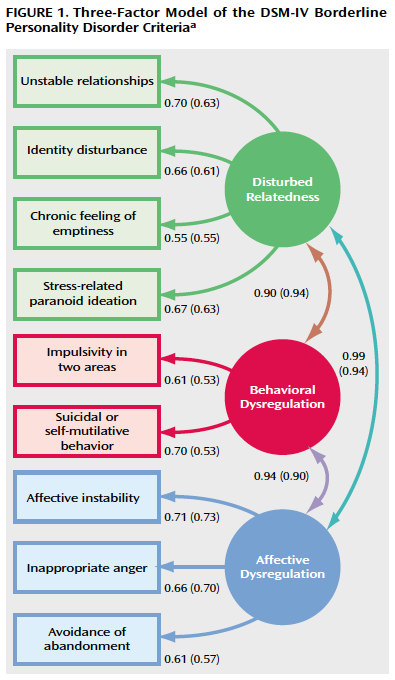
\includegraphics[width=0.5\textwidth]{011/image8.png}
\end{figure}

\subsubsection{Trattamento Cluster B}

I farmaci non sono curativi, ma aiutano a migliorare la funzionalitá
psichica.

\begin{itemize}
\item
  \textbf{Farmacoterapia}: soltanto mirata ai sintomi, quali:
\begin{itemize}
\item
  \emph{Impulsività/ disregolazione affettiva}: stabilizzatori, (AD)
\item
  \emph{Discontrollo impulsivo}: SGA, stabilizzatori {[}motrigina é il
  piú indicato; acido valproico; carbamazepina{]}
\item
  \emph{Pensiero quasi psicotico, derealizzazione}: SGA
\end{itemize}

Sono più utili nel mitigare i sintomi gli stabilizzatori dell'umore
(farmaco di prima scelta), perché agiscono sull'impulsività ed un po'
meno sull'instabilità affettiva, che ha connotazioni differenti nel
paziente borderline rispetto al paziente con disturbi dell'umore. Non si
usa litio e antidepressivi triciclici, perché hanno un basso indice
terapeutico e perché, se assunti in grandi quantità, possono causare la
morte per overdose: si preferiscono per questo motivo gli
antiepilettici.

\item
  \textbf{Psicoterapia a lungo termine} (4-5 tipi di psicoterapia che
  funzionano nei pazienti borderline, cioè che riducono i comportamenti
  suicidari ma non riducono gli altri fattori)
\item
  \textbf{Psicoeducazione a paziente e famiglie (}spiegare che né il pz,
  né i familiari sono colpevoli del disturbo, ma sono tutti responsabili
  della cura)
\end{itemize}

\subsection{Cluster C}

\paragraph{DP evitante}

Inibizione sociale per pervasivi sentimenti di inadeguatezza e timore di
critica o umiliazione. Soggetti timidi in ambito sociale che non escono
spesso perché cronicamente hanno timore in pubblico di provare vergogna.

Evitano i rischi e le attività che implicano un contatto interpersonale

Ritiro e timidezza: difese contro la vergogna (= paura di rivelare
aspetti di sé giudicati inadeguati)

Vergogna e ansia sociale diminuiscono con la famigliarità. Se conoscono
bene le persone, questa paura si calma. I disturbi d'interpersonalità
nel cluster C sono meno gravi che nel cluster B, perché il cluster C
riesce ad avere pochi amici.

\emph{\emph{Anamnesi personale di isolamento sociale e distanza forzata
da luoghi o circostanze; fobie, attacchi di panico. }}

\paragraph{DP dipendente}

Pervasivo bisogno di accudimento che induce ad un comportamento
sottomesso ed adesivo

Paura della separazione per incapacità ad assumersi autonomamente le
responsabilità della propria vita se soli cercano subito un'altra
relazione come fonte di rassicurazione, indipendentemente dalla qualità.
Sono Persone che possono stare anche in relazioni poco appaganti (anche
maltrattati) pur di stare con qualcuno. Spesso le persone che hanno
degli stalker come amanti, sono persone con questo tipo di DP. Il
paranoide è il partner ideale per le persone dipendenti e, raramente,
anche il narcisistico.

Condividono con il borderline la paura della separazione o
l'intolleranza all'abbandono. Tuttavia, nel dp dipendente, la paura
della separazione é strettamente collegata ad un'immagine negativa di
sé. I pz con dp dipendente pensano di non essere in grado di stare da
soli e sono grandiosi nella loro inadeguatezza (non riescono a pagare il
bollo dell'auto da soli, ad andare al lavoro da soli, a vivere in modo
indipendente la propria quotidianitá). Questi pz cercano il prossimo per
rassicurazione e non per bisgono della relazione.

N.B: spesso la dipendenza causa aggressività. Dipendenza= formazione di
compromesso (difende dall'ostilità che contemporaneamente viene
espressa).

\emph{\emph{L'anamnesi personale è di scarsa qualità nelle relazioni
sociali; disturbi depressivi e disturbi dell'adattamento}}

\paragraph{DP ossessivo-compulsivo}

Diagnosi differenziale con \emph{disturbo ossessivo--compulsivo o DOC},
caratterizzato dalla presenza di ossessioni e convulsioni che non sono
presenti nel disturbo ossessivo compulsivo della personalità. Non è
chiaro se prima dell'esordio di DOC ci sia sempre una condizione di
disturbo ossessivo-compulsivo della personalità: è presente in un 1/3
dei casi ma non è detto che ci sia, non siamo in presenza infatti di una
relazione di premorbosità.

Pervasive preoccupazione per l'ordine, la perfezione ed il controllo
mentale ed interpersonale (mondo interno).

Eccessiva attenzione ai dettagli e regole, a spese di flessibilità,
larghezza di vedute ed efficienza. Spesso a scapito dei sentimenti e
delle relazioni interpersonali autentiche (mondo esterno).

Eccessiva dedizione alla produttività a spese di attività di svago e
amicizie.

\begin{itemize}
\item
  Controllo di sentimenti propri o altrui (sono persone che nelle
  discussioni devono avere sempre ragione, perché loro sanno cosa è
  giusto o sbagliato)
\item
  Ricerca di perfezione (non del piacere)
\end{itemize}

Miglior funzionamento rispetto agli altri DP (vanno bene a lavoro).
Comorbidità: disturbi di panico, disturbi depressivi, DOC.

\subsubsection{Trattamento Cluster C}

\begin{itemize}
\item
  SSRI (più BDZ)
\item
  Psicoterapia
\begin{itemize}
\item
  DP evitante: cognitivo-comportamentale, psicodinamiche
\item
  DP dipendente e ossessivo compulsivo: psicodinamica
\end{itemize}
\end{itemize}

\subsection{Associazione di DP}

Tra i disturbi di personalità spesso c'è un'altra comorbidità: cioè una
persona non ha solo un disturbo ma ne ha di più. Com`è possibile avere
più DP?

Il DSM V ha fatto un passo in avanti, cambiando modo di classificare.
Oggi diciamo che il paziente ha un disturbo di personalità e ne
quantifichiamo il disfunzionamento e vediamo come si manifesta. Per
quantificare il disfunzionamento ci deve essere un danneggiamento
moderato o grave nel funzionamento della personalità e presenza di uno o
più tratti patologici di personalità (inflessibile, pervasivo, stabile
lungo il tempo cioè fin dalla tarda adolescenza o prima età adulta).

\documentclass[]{article}
\usepackage{lmodern}
\usepackage{amssymb,amsmath}
\usepackage{ifxetex,ifluatex}
\usepackage{fixltx2e} % provides \textsubscript
\ifnum 0\ifxetex 1\fi\ifluatex 1\fi=0 % if pdftex
  \usepackage[T1]{fontenc}
  \usepackage[utf8]{inputenc}
\else % if luatex or xelatex
  \ifxetex
    \usepackage{mathspec}
  \else
    \usepackage{fontspec}
  \fi
  \defaultfontfeatures{Ligatures=TeX,Scale=MatchLowercase}
\fi
% use upquote if available, for straight quotes in verbatim environments
\IfFileExists{upquote.sty}{\usepackage{upquote}}{}
% use microtype if available
\IfFileExists{microtype.sty}{%
\usepackage{microtype}
\UseMicrotypeSet[protrusion]{basicmath} % disable protrusion for tt fonts
}{}
\usepackage[unicode=true]{hyperref}
\hypersetup{
            pdfborder={0 0 0},
            breaklinks=true}
\urlstyle{same}  % don't use monospace font for urls
\IfFileExists{parskip.sty}{%
\usepackage{parskip}
}{% else
\setlength{\parindent}{0pt}
\setlength{\parskip}{6pt plus 2pt minus 1pt}
}
\setlength{\emergencystretch}{3em}  % prevent overfull lines
\providecommand{\tightlist}{%
  \setlength{\itemsep}{0pt}\setlength{\parskip}{0pt}}
\setcounter{secnumdepth}{0}
% Redefines (sub)paragraphs to behave more like sections
\ifx\paragraph\undefined\else
\let\oldparagraph\paragraph
\renewcommand{\paragraph}[1]{\oldparagraph{#1}\mbox{}}
\fi
\ifx\subparagraph\undefined\else
\let\oldsubparagraph\subparagraph
\renewcommand{\subparagraph}[1]{\oldsubparagraph{#1}\mbox{}}
\fi

% set default figure placement to htbp
\makeatletter
\def\fps@figure{htbp}
\makeatother


\date{}

\begin{document}

Isteria e Disturbo Algico

\emph{Isteria}

L'\textbf{isteria}, nota anche come \emph{disturbo di conversione} o
\emph{nevrosi isterica}, è una condizione caratterizzata dalla
\emph{presenza di uno o più sintomi neurologici}, come paralisi, cecità
o parestesie, che \emph{non possono essere spiegati da una malattia
neurologica o internistica nota}, ed in cui i sintomi d'esordio sono
tipicamente \emph{associati a fattori psicologici}.

La sindrome, oggi definita come disturbo di conversione, era in origine
associata alla sindrome ora nota come \emph{disturbo di somatizzazione}
e generalmente definita isteria, reazione di conversione o reazione
dissociativa. Attualmente si limita la diagnosi di disturbo di
conversione ai \emph{sintomi che coinvolgono una funzione volontaria
motoria o sensitiva}, cioè ai \textbf{sintomi neurologici}, e laddove il
medico non è in grado di spiegare i sintomi neurologici sulla base di
qualche malattia neurologica nota.

La diagnosi di disturbo di conversione richiede dunque che il medico
identifichi un'associazione necessaria e indispensabile tra la causa del
sintomo neurologico ed i fattori psicologici.

\textbf{Manifestazione Cliniche}

Clinicamente, il disturbo di conversione si manifesta con
\emph{paralisi}, \emph{cecità} e \emph{mutismo}, che sono i più comuni
sintomi di questa patologia, ma relativamente comuni sono anche i
\textbf{sintomi sensitivi}, come l'anestesia e le parestesie,
localizzate soprattutto agli arti. Tutti i sistemi sensitivi possono
essere coinvolti e la distribuzione delle alterazioni è solitamente
incongrua con quelle delle malattie neurologiche centrali o periferiche,
per cui si possono osservare le caratteristiche \emph{anestesie}
``\emph{a calza}'' o ``\emph{a guanto}'' oppure un'\emph{emianestesia
che inizia esattamente lungo la linea mediana}. I sintomi del disturbo
di conversione possono anche coinvolgere gli organi speciali di senso,
producendo \emph{sordità}, \emph{cecità} e \emph{visione} ``\emph{a
cannocchiale}'', e queste condizioni possono essere monolaterali o
bilaterali, tuttavia l'esame neurologico rivela che le vie sensoriali
sono integre, ad esempio, nella cecità da disturbo di conversione il
soggetto riesce a camminare senza riportare urti o danni, e le pupille
reagiscono alla luce, mentre i potenziali a livello corticale sono
normali.

Per quanto riguarda i \textbf{sintomi motori}, questi comprendono i
\emph{movimenti abnormi}, i \emph{disturbi della marcia}, al
\emph{debolezza} e la \emph{paralisi}. Possono essere presenti anche dei
\emph{tremori grossolani} e \emph{ritmici}, con \emph{movimenti
coreiformi}, \emph{tic} e \emph{sobbalzi}. I movimenti generalmente
peggiorano quando l'attenzione è focalizzata su di essi. Un peculiare
tipo di disturbo della marcia osservato nel disturbo di conversione è
l'\textbf{\emph{astasia-abasia}}, che è una \emph{deambulazione
vistosamente atassica}, \emph{vacillante}, accompagnata da
\emph{movimenti del tronco grossolani}, \emph{irregolari} e \emph{a
scatti} e da movimenti delle braccia a scatti e ondeggianti. I pazienti
con questi sintomi raramente cadono, e se questo succede, in genere non
si fanno male. Altri disturbi motori comuni sono le \emph{paralisi} e le
\emph{paresi}, che possono interessare uno, due o tutti e quattro gli
arti, anche se la distribuzione dei muscoli coinvolti non rispecchia
quella delle vie neurologiche. I riflessi sono normali, e non ci sono
fascicolazioni o atrofia muscolare, ed anche l'EMG è normale.

Si possono avere anche dei \textbf{sintomi simil-epilettici}, cioè delle
\emph{pseudocrisi epilettiche} che sono difficili da distinguere da
quelle reali, anche perché circa un terzo dei soggetti con pseudo crisi
ha anche un concomitante disturbo epilettico.

Infine, una particolare manifestazione clinica dell'isteria è il
fenomeno noto come ``\textbf{\emph{La Belle Indifférence}}'', cioè
l'\emph{atteggiamento del paziente inappropriatamente indifferente nei
confronti di un sintomo grave}, cioè il paziente non sembra preoccupato
da quello che appare invece come un deficit importante.

La diagnosi differenziale di disturbo di conversione non è affatto
semplice, poiché è alquanto complesso escludere in modo definitivo una
malattia organica, per cui la diagnosi differenziale va posta con
diversi \textbf{disturbi neurologici}, coi tumori cerebrali e le
patologie che interessano i gangli della base, nonché con
l'\textbf{ipocondria}, in cui il paziente non ha una vera e propria
perdita o alterazione del funzionamento, ed i disturbi somatici non sono
limitati ai sintomi neurologici, mentre si hanno dei caratteristici
atteggiamenti e forte convinzione della propria patologia.

\textbf{Trattamento dell'Isteria}

La risoluzione dei sintomi del disturbo di conversione è di solito
spontanea, anche se probabilmente è facilitata da una \emph{terapia di
supporto introspettiva}, per cui è fondamentale stabilire una relazione
terapeutica nella quale il terapista guidi con autorità ed assista il
paziente, per cui spesso si ricorre alla psicoterapia psicodinamica o a
forme brevi di psicoterapia.

\emph{Disturbo Algico}

Il \textbf{disturbo algico} (noto anche come \emph{disturbo da dolore
somatoforme} o \emph{disturbo da dolore psicogeno}), è definito dalla
presenza di \textbf{\emph{dolore}} che è ``l'oggetto principale
dell'attenzione clinica'', per cui il sintomo principale è proprio il
dolore, in uno o più distretti anatomici, che non viene completamente
spiegato da un'affezione medica non psichiatrica o neurologica.

I sintomi algici sono peraltro associati a \emph{disagio emotivo e a
limitazione del funzionamento del paziente}, ed il disturbo ha una
\emph{plausibile relazione causale con fattori psicologici}; questa
forma di disturbo, peraltro, è due volte più comune nelle donne che
negli uomini, e l'età di esordio più frequente è tra la IV e V decade di
vita, forse perché la tolleranza al dolore si riduce con l'età.

\textbf{Manifestazioni Cliniche}

I pazienti con disturbo algico non costituiscono un gruppo uniforme dal
punto di vista clinico, ma piuttosto sono un gruppo eterogeneo con vari
dolori, come \emph{lombalgia}, \emph{cefalea}, \emph{dolore facciale
atipico} e \emph{dolore} \emph{cronico pelvico}. Questi dolori possono
essere post-traumatici, neuropatici, neurologici, iatrogeni o
muscolo-scheletrici, tuttavia, per soddisfare la diagnosi di disturbo
algico occorre che sia presente un fattore psicologico che possa essere
considerato significativamente correlato ai sintomi algici e alle loro
ramificazioni. I pazienti con questo disturbo hanno spesso una
\emph{lunga storia di cure mediche e chirurgiche}, con consulti presso
molti medici e \emph{richiesta di numerose terapie}, e in alcuni casi
possono diventare anche piuttosto insistenti, arrivando a richiedere gli
interventi, e sono \emph{completamente coinvolti dalla preoccupazione
per il dolore}, riferendolo come \textbf{fonte di ogni loro disagio e
sofferenza}.

Inoltre, i pazienti con disturbo algico possono avere un quadro clinico
complicato da un disturbo correlato a sostanze, perché \emph{tentano di
ridurre il loro dolore con alcol o droghe}, mentre tipici sono anche
alcuni disturbi dell'umore, come la distimia o gli episodi depressivi
maggiori, che in questi casi possono presentarsi nella forma definita di
``\textbf{depressione mascherata}'' della psicopatologia classica.

\end{document}

\section{Disturbi del Comportamento Alimentare}

\subsection{Definizione e caratteristiche generali}

I \textbf{disturbi del comportamento alimentare} (\textbf{DCA}), secondo
le ultime classificazione del DSM-V, sono un gruppo molto ampio ed
eterogeneo di disturbi psichiatrici, che include al suo interno alcune
forme principali, nello specifico:

\begin{itemize}
\item
  l'\emph{anoressia nervosa} (AN)
\item
  la \emph{bulimia nervosa} (BN),
\item
  ma anche altre forme psichiatriche come il \emph{BED (Binge Eating
  Disease)}, il \emph{picacismo}, il \emph{disturbo di ruminazione} ed
  altre forme generalmente indicate come \emph{OSFED} (Other Specified
  Feeding or Eating Disorders).
\end{itemize}

Per definizione, inoltre, non si può parlare propriamente di DCA se non
sono rispettati i seguenti 4 criteri:

\begin{itemize}
\item[1.]
  Dev'essere presente un \textbf{disturbo o un'alterazione delle
  abitudini alimentari o dei comportamenti specificamente volti al
  controllo del peso}. Cioè come e quanto un soggetto mangia e quindi
  quanto e come un soggetto controlla il proprio peso.
\item[2.]
  Dev'essere presente nel paziente \textbf{\emph{un'eccessiva influenza
  della forma e del peso corporeo sui livelli di autostima}} (questo
  punto è quello fondamentale per comprendere i meccanismi alla base dei
  DCA, e prende il nome di \textbf{disturbo dell'immagine corporea}).
  Tutte le altre cose che generalmente sostengono l'autostima di una
  perosna sana per il paziente affetto da DCA perdono di significato. Se
  non c'è questo criterio non si può parlare di disturbo psichiatrico
\item[3.]
  I precedenti due punti devono causare un \textbf{deterioramento
  clinicamente significativo della salute fisica o del funzionamento
  psico-sociale del paziente} (come in molti altri casi psichiatrici, un
  certo atteggiamento o convinzione non può essere considerata
  patologica se non causa un cambiamento significativo del funzionamento
  del soggetto).
\item[4.]
  Dev'essere \textbf{esclusa la presenza di altre eventuali patologie
  internistiche o psichiatriche alla base}.
\end{itemize}

Tra questi quattro punti, quello su cui si deve focalizzare l'attenzione
è il secondo, cioè il disturbo dell'immagine corporea, in quanto
costituisce la caratteristica psico-patologica principale dei DCA.

\subsection{Classificazione}

I DCA vengono generalmente suddivisi in:

\begin{itemize}
\item
  \textbf{anoressia nervosa} (AN, con le due varianti AN-R e AN-P),
\item
  \textbf{bulimia} \textbf{nervosa}
\item
  i \textbf{DCA NAS} (Non Altrimenti Specificabili), che non rientrano
  né nell'AN, né nella BN.
\end{itemize}

\textbf{\emph{ETIMOLOGIA:}}

Se si va a guardare ai termini letterali delle patologie:

\begin{itemize}
\item
  ``anoressia'' starebbe a significare ``\emph{assenza di appetito}'',
\item
  ``bulimia'' vorrebbe dire ``\emph{fame da bue}'',
\end{itemize}

ma in realtà questi termini appaiono fuorvianti, perché in queste
patologie psichiatriche non si ha un'alterazione dell'appetito, sebbene
i pazienti arrivino spesso a negare il senso di fame, ma quello che
risulta anomalo è il disturbo dell'immagine corporea, in base al quale
l'autostima del paziente non può fare a meno di dipendere dalle sue
caratteristiche più strettamente fisiche, ovvero il peso e la forma del
corpo.

\subsection{Epidemiologia e mortalità}

Per quanto riguarda l'aspetto epidemiologico dei DCA, sono disturbi la
cui prevalenza nelle popolazioni a rischio, in particolare negli
adolescenti, sono in aumento:

PREVALENZA: per l'anoressia nervosa la prevalenza stimata è dello
\emph{0,5-1\%}, mentre per la bulimia nervosa la prevalenza varia
\emph{tra l'1 e l'8\%}.

ETA':Si tratta in ogni caso di disturbi che si sviluppano in genere
durante la \emph{seconda decade di vita,}

SESSO: Hanno una \emph{preferenza per il sesso femminile} (rapporto
maschi/femmine di circa 0,5 a 9,5 per l'anoressia nervosa, passa ad 1 a
4 per la bulimia)

TASSO DI GUARIGIONE: di questi pazienti meno del 50\% riesce a guarire
completamente

TASSO DI MORTALITA': il tasso di mortalità si attesta sul \emph{5-20\%},
cioè il valore più alto tra le varie patologie psichiatriche, assieme
all'abuso di sostanze, e questo perché nei DCA si ha un deterioramento
fisico notevolmente maggiore, a cui si va ad aggiungere anche il rischio
di suicidio, che tuttavia contribuisce solo per il 2\% a tutte le morti
dovute a DCA

\subsection{Eziologia}

Dal punto di vista dell'eziologia, l'origine dei DCA è complessa e
ancora non del tutto definita, sebbene vi siano due modelli principali
eziopatogenetici:

\begin{itemize}
\item
  \textbf{\emph{MODELLO BIO-PSICO-SOCIALE:}}

  Il primo è il \textbf{modello bio-psico-sociale}, in base al quale
  diversi fattori biologici, psicologici, familiari e socio-culturali si
  combinano in modo additivo per produrre una patologia del
  comportamento alimentare. Anche quando si era parlato dei disturbi
  della personalità avevamo detto che questo modello non ci soddisfa del
  tutto perché ci da un'idea del ``frullatore'', ossia frullando insieme
  questi fattori salta fuori la patologia. Abbiamo bisogno di un modello
  che ci spieghi qualcosa in più.
\item
  \textbf{\emph{MODELLO DIATESI STRESS:}}

  Il secondo modello, oggi più accreditato, è il \textbf{modello
  diatesi-stress}, in base al quale esiste una \emph{predisposizione
  biologica}, su base multigenica, che determina una
  \emph{predisposizione ai DCA e ne determina anche la forma} (ad
  esempio la vulnerabilità all'AN piuttosto che alla BN), ed è poi
  un'eventuale esposizione ad \emph{eventi stressanti} a determinare se
  il disturbo si svilupperà o meno. Quindi questo modello,
  vulnerabilità-stress, recita che una predisposizione biologica, ad
  esempio genetica, determina se io ho rischio di sviluppare un disturbo
  alimentare e in particolare se ho il rischio di sviluppare AN
  piuttosto che BN. La predisposizione da sola non fa il disturbo.
  L'esposizione a momenti di vita stressanti che possono essere sia
  psicologici (interni) che ambientali, determina a partire dalla
  predisposizione se il disturbo si svilupperà o meno. E' un po' la
  teoria gene-ambiente. Questo vuol dire che noi tutti differiamo nella
  probabilità di sviluppare un disturbo alimentare e dunque nella
  ``sensibilità'' agli eventi stressanti tipicamente associati
  all'eziologia di un dca.
\end{itemize}

Ovviamente, oltre ai fattori predisponenti su base genetica, ve ne sono
diversi altri di natura ambientale e culturale, Il fattore cardine che
dobbiamo spiegare nell'eziologia di questo disturbo è
\textbf{l'insoddisfazione per il corpo} che è una caratteristica comune
ad entrambe le patologia in essere.

Questa insoddisfazione per il corpo è dovuta anche a \textbf{FATTORI DI
TIPO CULTURALE} che inseriamo nei fattori di rischio di tipo ambientale
e sociale nei modelli precedentemente accennati.

In prevalenza questi disturbi hanno incidenza più alta in dei posti dove
c'è abbondanza di cibo, ma culturalmente viene \textbf{idealizzata la
magrezza} poiché essendoci rischio di obesità essa non è considerata
solo ``bella'' ma anche ``giusta'' perché è sana. Sana in quanto
l'obesità, l'ipercolesterolemia, il sovrappeso ecc... fanno morire un
sacco di gente da noi. I fattori di rischio culturali non sono solo
quelli passati in televisione (la modella magrissima che sfila), ma
anche il pediatra che a ragione ``prescrive'' al bambino in sovrappeso
una dieta, essendo tale patologia un fattore di rischio specie se
insorge in età pediatrica. Dunque queste culture danno alla magrezza non
solo un valore estetico, bensì anche un valore etico. Ci spiegano anche
la prevalenza in adolescenza perché è un momento in cui volente o
nolente il fisico cambia e il peso si fa sentire sotto forma di presa in
giro da parte dei coetanei o sotto forma di cambiamenti dovuti al
menarca. E' un età in cui insorgono anche cambiamenti dovuti all'enfasi
del soggetto sul corpo perché è importante per essere accettati dagli
altri, per trovare un fidanzati.

Altri fattori di rischio sono \textbf{l'influenza dei coetanei} (sono
state osservate delle piccole epidemie di anoressia in delle classi) e
\textbf{l'influenza dei media}. E' stato visto che questi fattori sono
tutti correlabili nell'insorgenza dei disturbi alimentari. Ce lo spiega
anche il fatto che l'incidenza di queste patologie nei paesi occidentali
è aumentata tra il 1930 e il 1980, con l'incremento dell'abbondanza e
della possibilità dunque di aumentare di peso

Quello che questi fattori culturali non ci spiegano è la stima
dell'\textbf{EREDITABILITÀ}: la proporzione di varianza fenotipica
ascrivibile a cause genetiche è alta. Se questi disturbi dipendessero
solo da fattori di rischio culturali, non ci aspetteremmo
l'ereditarietà. Questo vuol dire che la società ha colpa, ma c'è
qualcosa di più profondo sotto. Possiamo fare molto in termini di
prevenzione primaria, ma non tutto. Parliamo di cose che hanno a che
fare anche con la biologia, non sono solo dei capricci del soggetto che
segue i dettami della moda.

Dell'insoddisfazione per il corpo chi più e chi meno ne soffrono tutti
coloro i quali non abbiano una forma fisica invidiabile e questo è
sicuramente dovuto a fattori culturali, però essa da sola non fa un DCA.

Tra i fattori genetici, i principali sono i fattori che regolano il
\textbf{temperamento}, infatti si è visto che i DCA sono associati a
particolari tratti comportamentali (ad esempio, l'AN è tipica di
soggetti perfezionisti e dalla volontà forte, finanche ossessiva, mentre
la BN è più comune in soggetti impulsivi e con affettività negativa).

Infine abbiamo i \textbf{FATTORI FAMILIARI}, che sono in realtà alquanto
aspecifici, poiché presenti anche in molte altre patologie
psichiatriche; tra questi vanno ricordati la familiarità psichiatrica,
la storia di DCA materna, l'abuso fisico o sessuale e una storia
infantile di scarse cure parentali ma con elevato controllo
(\textbf{fenomeno dell'Over Protection}).

Per esempio: madre affetta da DCA non solo trasmette alla figlia la
predisposizione alla malattia, ma la sottopone in seguito a commenti
riguardo la sua forma e peso corporei.

Per esempio: L'ambiente familiare, quello del controllo senza affetto:
genitori iperprotettivi che fanno fatica ad accettare che i figli
facciano le cose in autonomia ma allo stesso tempo poco empatici, poco
capaci di dare affetto. In una percentuale non indifferente di casi c'è
abuso sessuale o fisico nell'infanzia.

\subsection{Esordio}

Ma come si sviluppa un disturbo dell'alimentazione? Alla base, come
accennato, vi sarebbe un \emph{personalità} \emph{predisponente},
caratterizzata da un \textbf{SENTIMENTO PERVASIVO DI INSICUREZZA E DA UN
SENSO DI SÉ INSTABILE}, che si accentua particolarmente all'inizio
dell'adolescenza; questi giovani pazienti sono spesso in leggero
sovrappeso, e vengono stimolati dai parenti, dai coetanei o addirittura
dal medico di medicina generale a perdere un po' di peso, essenzialmente
per prevenire ulteriori problemi fisici.

Quando questi fattori di rischio si uniscono in modo non casuale, per
via delle correlazioni gene-ambiente di cui prima, il soggetto si
affaccia all'adolescenza con una cosa che ha la caratteristica nucleare
di tutti i disturbi del comportamento alimentare, senza questa
caratteristica \textbf{l'insoddisfazione per il corpo} non si trasforma
in dca ed è indicata con il termine inglese ``unaffectiveness'' che
viene tradotto con l'italiano \textbf{\emph{\emph{``inadeguatezza}}''}.
E' un senso pervasivo di non sapere chi si è in ogni data circostanza e
non sapere come essere efficaci: come cambiare l'ambiente che hanno
intorno se non gli piace, come parlare con gli altri; queste persone vi
dicono ``\emph{mi sento non all'altezza}'', ``\emph{mi sento non
adeguato}'' davanti a tutto: scuola, genitori, amici.

Quindi c'è un \emph{problema di identità e di controllo del mondo
esterno}, non si sentono ``equipaggiati''. Ciò che per gli altri è
automatico e spontaneo per loro è impossibile. E' solo con questi
presupposti che arrivando all'adolescenza, incontrando i fattori
culturali che loro trasferiscono la ``soluzione'' al loro problema con
la ricerca estrema della magrezza: \emph{``se io riesco a controllare il
mio peso e ad essere magro, non avrò più questi problemi''}.

Questi pazienti affermano che prima non erano buoni a nulla ma ora poi
dimagrendo valgono. Questo è il punto cardine per capire i DCA e le
difficoltà di trattamento: \textbf{nessun peso è abbastanza basso}
(disturbo dell'immagine corporea) per i pazienti non è un problema ma
per loro è la soluzione. Di fatto conferisce senso e significato alla
vita del paziente e rappresenta la via finale dei fattori di rischio
osservato.

Il \textbf{disturbo dell'immagine corporea} comporta che tutta la
soddisfazione di sé dipende solo e soltanto dal peso corporeo che rende
la vita del paziente più semplice,più efficace e più sicura. Trova una
soluzione maladattativa alla sua sofferenza, confusione e senso di
inadeguatezza \emph{identificando tutto se stesso con il suo peso:}
valgo solo se sono sempre più magra. E' per questo che si tratta di una
patologia psichiatrica.

Trovandosi davanti ad un medico che sia psichiatra o internista che
sostiene che bisogna che il paziente riprenda peso per aver salva la
vita, il paziente diventa non collaborante perché sente che cercano di
sottrargli l'unica certezza della vita. E' una lotta incredibile.

Caso clinico: \emph{ragazzino di 13 anni con un BMI di 12.5 che
presentava iperattività (vedremo che è un meccanismo di compenso), calo
di peso repentino che con una frequenza di 34 bpm è scappato veloce come
il vento per i viali dell'ospedale tanta era la disperazione con cui si
opponeva al ricovero, una questione di vita o di morte per lui. I
genitori son dovuti corrergli dietro per recuperarlo, finché non è stato
predisposto il ricovero è stato letteralmente piantonato in casa con i
genitori ed i nonni perché in bagno di notte con la luce spenta saltava
nella doccia. Quando è arrivato in ospedale aveva già un versamento
pericardico e saltava ancora. Ridurre il più possibile il peso anche a
rischio di gravissime conseguenze per loro è davvero una questione di
vita o di morte.}

\subsection{Diagnosi}

Anche se non tutti i futuri medici faranno gli psichiatri potrebbero
ugualmente essere utili per riconoscere i prodromi di questi disturbi,
quindi per fare una diagnosi precoce si parte dall'\textbf{anamnesi}:

\begin{itemize}
\item[1.]
  \emph{Familiarità per disturbi psichiatrici} che per i soggetti che
  sviluppano AN in genere sono disturbi d'ansia o disturbo
  ossessivo-compulsivo, nel caso di BN si tratta invece di disturbi
  dell'umore, abuso di alcol o di altre sostanze.
\item[2.]
  Per entrambi c'è \emph{DCA materno} con \emph{basso peso alla nascita}
  perché la madre ha un DCA parzialmente guarito.
\item[3.]
  Ci possono essere \emph{complicanze neonatali} e \emph{problemi
  alimentari} nell'infanzia come rifiuto di alcuni cibi, alimentazione
  selettiva, disturbi gastroenterologici, ritardo nella crescita.
\end{itemize}

In adolescenza, quelli che necessiterebbero di uno \textbf{screening}
sono:

\begin{itemize}
\item
  Soggetti a bassa crescita,basso peso e con disturbi mestruali. Il
  ginecologo per prima cosa prescrive la pillola ed è un grave errore,
  infatti va prima indagato se c'è un DCA.
\item
  Soggetti che si presentano con vomito e disturbi gastroenterologici
  non spiegati.
\item
  Pazienti affetti da diabete mellito di tipo I che presentano anche
  predisposizione per DCA (sono particolarmente a rischio perché si
  manifesta con perdita marcata del peso finché non si inizia il
  trattamento e il peso risale e si fa un regime dietetico controllato,
  di questo il paziente non sarà felice).
\item
  Soggetti che si presentano con disturbi depressivi od ossessivi (la
  psichiatria dell'adolescenza è più complicata, il paziente è il
  crescita!).
\end{itemize}

Se sarete medici di medicina generale, sarà importante per fare diagnosi
precoce saper riconoscere i segnali e approfondire le situazioni di
questi ragazzi e monitorare la crescita, dando molta attenzione alla
preoccupazione della gente che il paziente ha intorno.

La \emph{\emph{modalità di esordio}} più comune parte da una
\textbf{condizione di lieve sovrappeso} nell'adolescenza che innesca
l'inizio di una dieta e qui non siamo nella patologia, la dieta è giusta
e magari gli è stata data per una serie di ottimi motivi dal pediatra.

La situazione si \emph{\emph{sviluppa}} perché in questi soggetti ciò
che gli era stato prescritto come dieta dopo un po' lo dimenticano e
cominciano a ridurre sempre di più a partire dallo schema dietetico
l'apporto calorico.

Arrivano a mangiare sempre meno, il peso diminuisce molto e si assiste
alla \textbf{fase di ``luna di miele''} delle anoressiche a cui tutte
vorrebbero tornare: aumenta il tono dell'umore ed entrano in una
\textbf{fase ipomaniacale} (non è un episodio maniacale vero è proprio)
in cui la sensazione è quella di avere più forza, più energia, più
voglia di fare molte cose e si ha la sensazione che tutto venga
piuttosto facile. Per questo soggetto questa non è una sensazione usuale
e per la prima volta sente l'efficacia personale e interpersonale e non
chiederà di certo un trattamento.

Le cose progrediscono e si struttura il \textbf{disturbo dell'immagine
corporea}, : l'insicurezza e l'insoddisfazione del paziente vengono
placate dal controllo di quelle che sono le caratteristiche fisiche
immediatamente controllabili, cioè il peso e la forma del corpo:ossia il
paziente inizia ad avere la smania di controllare il suo peso e di
dimagrire sempre di più per potersi sentire adeguato. Per stare bene i
soggetti si chiudono in questa ``gabbia d'oro'' fatta solo del controllo
del peso. Il paziente giunge alla convinzione, spesso inconscia, che
controllando il proprio peso possa controllare tutti gli aspetti della
sua personalità che trova inadeguati, e ciò conferisce alla vita del
paziente un senso ed un significato che prima mancavano, in quanto
questi identifica tutta la sua persona nel peso e nella forma del corpo.
Qui siamo già entrati nella patologia.

Per mantenere il peso più basso possibile si strutturano le
\textbf{strategie per mantenere basso il peso corporeo},questi soggetti
fanno tutto quello che possono per ricercare la magrezza con i mezzi più
svariati:

\begin{itemize}
\item[1.]
  Il paziente cerca di perdere ulteriormente peso, in genere
  organizzando un'\emph{iperattività fisica pianificata e ritualistica}
  (cioè finisce per cercare il modo più faticoso di fare ogni cosa): è
  comune fare iperattività sistematica e ritualizzata ossia scelgo il
  modo più faticoso per fare tutte le cose (es: 8 piani di scale a piedi
  tutti i giorni invece di prendere l'ascensore).
\item[2.]
  Gli \emph{schemi alimentari iniziano a diventare rigidi}, fissi,
  stereotipati e di una povertà estrema e il paziente sceglie una serie
  di alimenti che considera accettabili per mantenere basso il peso. A
  questo punto manca qualsiasi tipo di spontaneità nelle scelte
  alimentari che sono dettate solo da questa necessità di controllo del
  peso e dunque dal fatto di accettare di mangiare solo ciò che non
  mette ansia legata al timore indicibile di ingrassare.
\end{itemize}

Altra caratteristica tipica di questi pazienti è la \textbf{continua
negazione della fame}, la quale viene appunto definita come latente e
negata, e determina l'insorgenza di ossessioni sul cibo e sui regimi
alimentari, che sono ovviamente egodistonici.

Ovviamente se uno non mangia la prima cosa che gli viene è la fame, a
loro non manca l'appetito almeno non nelle prime fasi. Nelle ultime
invece vengono davvero compromessi i meccanismi di fame e di sazietà.

Loro negheranno questa fame anche se la sentono e rispunterà sempre
sotto forma di \textbf{ossessioni} (ideazioni, pensieri, immagini,
impulsi egodistoniche intrusive) sul cibo e sui regimi alimentari da
quando si alzano alla sera quando vanno a letto. A questa cosa ci si può
attaccare per convincerli a farsi curare perché è una situazione molto
disturbante per il soggetto.

Un altro modo che la fame ha di riemergere nella metà dei casi è sotto
forma di \textbf{crisi bulimica}. Questa lotta tra la volontà del
paziente ed il senso di fame può quindi evolvere in due diversi
disturbi:

\begin{itemize}
\item
  nel 50\% circa dei casi il senso di fame ha la prevalenza, spesso a
  causa anche del temperamento impulsivo del paziente, e si hanno
  \textbf{crisi bulimiche} con abbuffate di cibo e perdita di controllo,
  a cui fanno poi seguito degli spiccatissimi sensi di colpa che vengono
  ``espiati'' tramite il vomito autoindotto, l'abuso di diuretici e
  lassativi e l'uso di sostanze anoressizzanti, per cui questi pazienti
  soffrono di \textbf{\emph{bulimia nervosa}} o di
  \textbf{\emph{anoressia nervoso di tipo purging}} (la differenza
  risiede essenzialmente nella diversità di frequenza delle abbuffate),
\item
  mentre nel restante 50\% circa dei pazienti la volontà del paziente
  riesce a prevalere sul senso di fame, ed il paziente \emph{mantiene le
  restrizioni caloriche}, ma sempre senza saltare i pasti, ed il peso
  continua a scendere, e tale comportamento è caratteristico
  dell'\textbf{\emph{anoressia di tipo restrittivo}}.
\end{itemize}

La caratteristica che divide in due questa classe di soggetti è
l'abbuffata che caratterizza i soggetti che hanno disturbi bulimici e
invece i soggetti che hanno disturbi da anoressia nervosa restrittiva
non si abbufferanno mai.

L'esordio dal punto di vista sintomatologico è comune per tutti, ma ciò
che fa andare alcuni individui verso un disturbo ed altri verso l'altro
è la predisposizione genetica che abbiamo visto poco prima, ossia la
familiarità con patologie psichiatriche diverse.

La possibilità di sviluppare l'AN-R o la BN o la AN-P dipendono quindi,
come già accennato, dalle caratteristiche temperamentali del paziente:
in generale, i pazienti con caratteristiche genetiche di ipercontrollo,
ossessività e rigidità tendono a sviluppare l'anoressia restrittiva,
mentre chi ha delle caratteristiche di discontrollo impulsivo e
instabilità affettiva tendenzialmente seguirà la via dei disturbi di
tipo bulimico.

L'ambiente non determina la transizione da un disturbo all'altro ma è
importante istruire i genitori su quei comportamenti da non tenere con
questi ragazzi perché potrebbe spingerli a mangiare per senso di colpa
verso i genitori ond'evitare poi andare a vomitare perché ``non se lo
possono permettere''.

\subsection{Criteri diagnostici dell'anoressia nervosa}

Per poter parlare propriamente di anoressia nervosa, devono essere
soddisfatti alcuni criteri dettati dal DSM:

\begin{itemize}
\item
  \textbf{Rifiuto di mantenere il peso corporeo al di sopra o in
  corrispondenza del minimo peso ideale per l'età e la statura del
  paziente}, che in genere corrisponde all'\textbf{85\%} del peso
  normale per quel paziente. Non c'è un cutoff preciso, ma già sotto 18
  di BMI in presenza degli altri sintomi si può parlare di sottopeso
  clinicamente significativo.
\item
  \textbf{Intensa paura di acquistare peso o di ingrassare anche se si è
  marcatamente sottopeso}.
\item
  \textbf{Alterazione del modo in cui il paziente vive il peso e la
  forma corporea (disturbo dell'immagine corporea), oppure un'eccessiva
  influenza del peso e della forma sui livelli di autostima o rifiuto di
  ammettere la gravità della situazione di sottopeso}.
\item
  Nel DSM-IV era inclusa come criterio diagnostico anche
  l'\textbf{amenorrea}, cioè l'assenza di almeno 3 cicli mestruali
  consecutivi, ma nel DSM-V questo criterio è stato rimosso, sia perché
  non lo si può ovviamente applicare ai soggetti di sesso maschile, sia
  perché nelle pazienti molto giovani può essere difficile identificare
  tale condizione.
\end{itemize}

\subsubsection{Classificazione}

Ci sono due sottotipi di AN:

\begin{itemize}
\item[1.]
  l'\textbf{anoressia nervosa restrittiva} (\textbf{AN-R}) è tipica dei
  soggetti con ipercontrollo, che continuano le restrizioni caloriche
  nonostante il notevole senso di fame,
\item[2.]
  l'\textbf{anoressia nervosa di tipo purging} (\textbf{AN-P}): si hanno
  delle abbuffate o delle condotte di eliminazione, quali vomito
  autoindotto, abuso di lassativi, e questi atteggiamenti possono
  ricordare quelli della bulimia nervosa.
\end{itemize}

DD CON BULIMIA NERVOSA da cui si distinguono per la \emph{frequenza
delle abbuffate} (sporadiche nell'AN-P, molto più comuni nella BN), il
\emph{peso} (nella BN il paziente è spesso normopeso o di poco
sottopeso, mentre nell'AN-P il paziente è marcatamente sottopeso), la
\emph{possibile assenza di amenorrea} (che comunque non è più un
criterio valido nel DSM-V) e per il fatto che nell'anoressia purging
\emph{le abbuffate possono non essere reali}, cioè il paziente cede alla
fame e mangia, magari poco, però poi si sente in colpa come se si fosse
abbuffato in maniera enorme, perché comunque è venuto meno al suo
obiettivo.

\emph{\emph{Grado di Gravità:}}

Per il criterio di gravità in genere si usa il BMI:

\begin{itemize}
\item[1.]
  Leggera \textless{}17
\item[2.]
  Moderata tra 16 e 17
\item[3.]
  Grave tra 15 e 16
\item[4.]
  Estrema \textless{}15
\item[5.]
  Regime di emergenza: si fa riferimento ad un BMI di 14, anche se non
  si fa riferimento solo a quello.
\end{itemize}

Ci possono essere forme sotto soglia per cui il soggetto può aver avuto
un periodo di AN che poi è andato in regressione grazie al trattamento e
può avere alcuni dei sintomi ma non tutti. In questo caso si parlerà di
remissione parziale.

E' importante anche capire che una persona che fa tutte queste cose
oltre al calo drammatico del peso ha anche altre ripercussioni fisiche e
psicologiche.

\emph{\emph{Ripercussioni psicologiche}}: \emph{sintomi depressivi,
ansiosi o ossessivi}, \emph{isolamento sociale} (il pensiero del
paziente è del tutto focalizzato sul controllo del peso, per cui si ha
un disinteresse verso gli altri e inoltre le condotte di controllo
sull'alimentazione o le abbuffate e il vomito autoindotto non permettono
una vita sociale normale: i pensieri fissi sul cibo non permettono di
fare serenamente le normali attività come andare al cinema e in più è
impossibile andare a prendere una pizza con gli amici, mangiare in
pubblico è un'impresa), \emph{tratti perfezionistici maladattativi}, con
uno \emph{stile cognitivo molto rigido}, \emph{disinteresse sessuale} e
\emph{pensiero magico}. sintomi depressivi, ansiosi e oppressivi,
saranno isolati socialmente).

Alcune caratteristiche cliniche sono esacerbate o causate dallo stato di
denutrizione e l'unico modo per curare l'anoressia è la renutrizione.
Qualsiasi farmaco prima della renutrizione è inutile o addirittura
dannoso. Anche una valutazione psicologica non è completa se prima non è
stato renutrito, ha un modo di pensare diverso dal suo modo usuale,
alterato perché c'è stato un cambio di personalità.

\emph{\emph{Ripercussioni fisiche}}: Clinicamente molto rilevanti sono
poi le \textbf{\emph{manifestazioni internistiche}}, che possono essere
estremamente gravi e potenzialmente letali. In corso di AN gli apparati
coinvolti sono praticamente tutti:

\begin{itemize}
\item
  \textbf{Apparato cardiovascolare}: E' un criterio valutato per
  l'ospedalizzazione; è comune l'\emph{ipotensione ortostatica}, spesso
  associata ad \emph{acrocianosi}, \emph{alterazioni dell'ECG},
  \emph{bradicardia}, \emph{allungamento del tratto QT a causa
  dell'ipopotassemia} e \emph{predisposizione alle aritmie} (sono la
  prima causa di morte). Per questo alcuni farmaci se il paziente non è
  stato renutrito sono potenzialmente dannosi perché gli antipsicotici
  per cui c'è lieve evidenza che aiutano nell'iperattività fisica per
  consumare calorie, aumentano il tratto QT, quindi capite il rischio.
\item
  \textbf{Apparato muscolo-scheletrico}: deplezione della massa
  muscolare e osteopenia che può progredire fino ad osteoporosi e può
  causare fratture. Questo succede perché non vengono sintetizzati gli
  estrogeni, cioè l'amenorrea nei soggetti di sesso femminile è dovuta
  al fatto che l'ipotalamo non manda dei messaggi per secernere in modo
  pulsatile, come sarebbe atteso dopo la pubertà, le gonadotropine e
  dunque gli ormoni ovarici che servono anche a fissare il calcio dal
  sangue alle ossa, dunque dopo sei mesi di amenorrea le linee guida
  dicono che bisogna fare la MOC (Mineralometria Ossea Compiuterizzata)
  anche se il soggetto ha 15 anni
\item
  \textbf{Tiroide}: si mette un po' a riposo, c'è la sindrome della
  tiroide che sta bene ma si ammala (euthyroid sick syndrome) e
  aumentano i livelli periferici di rT3 che dimostra che la tiroide
  funziona ma che l'ormone tiroideo viene inattivato in periferia poiché
  l'ormone tiroideo aumenta il metabolismo e il corpo si difende da
  questo poiché è l'ultima cosa di cui ha bisogno in questa situazione;
\item
  \textbf{Apparato gastrointestinale}: stipsi poiché mangiando
  pochissimo hanno anche poco materiale da espellere. Per i soggetti
  anoressici questa sensazione di gonfiore addominale è inaccettabile e
  questo può portare anche all'abuso dell'uso di lassativi;
\item
  \textbf{Pelle}: spesso cosparsa di peluria lunga e sottile chiamata
  lanugo, specie in fase avanzata del disturbo. Questo accade perché non
  sono più prodotti gli estrogeni e sono loro che con lo sviluppo dei
  caratteri sessuali secondari stimolano la crescita dei peli più in
  alcuni posti che in atri;
\item
  \textbf{Sistema Nervoso Centrale:} abulia, apatia, deterioramento
  cognitivo soprattutto in fasi croniche avanzate ed è questo il motivo
  per cui è quasi impossibile comunicare con loro prima di averli
  renutriti. \textbf{SNC} si riscontra \emph{deterioramento cognitivo},
  \emph{abulia}, \emph{apatia}, \emph{umore depresso e disforico}, ed
  \emph{idrocefalo ex-vacuo} per riduzione della sostanza cerebrale.
\item
  \textbf{Apparato riproduttivo}; si hanno \emph{amenorrea},
  \emph{arresto o regressione dello sviluppo sessuale},
  \emph{ipoestrogenemia} e \emph{pattern prepuberali di secrezione di
  FSH ed LH}
\item
  \textbf{Nel} \textbf{sistema emopoietico} si sviluppa \emph{anemia}
\item
  \textbf{Nel sistema endocrino-metabolico} si riscontra
  \emph{ipercortisolemia}, \emph{anomalie elettrolitiche} e
  \emph{sindrome da rT3} (reverse T3)
\item
  A \textbf{livello urinario} si riscontra \emph{iperazotemia},
  \emph{calo della GFR} e \emph{nefropatia ipovolemia}..
\end{itemize}

\subsection{Diagnosi differenziale}

La \textbf{\emph{diagnosi differenziale}} va posta con \emph{gravi
deperimenti secondari a malattie organiche}, \emph{disturbi endocrini o
patologie gastro-intestinali} (RCU, ulcera peptica, tumori,
enterocoliti), nonché altre patologie psichiatriche, quali la
\emph{depressione maggiore} (soprattutto la forma melanconica c'è
iporessia), la \emph{schizofrenia con delirio di veneficio} (si
convincono che gli altri vogliano avvelenarli) ed alcuni \emph{disturbi
fobici} con attacchi di panico situazionali con paura di ingoiare per
rischio di soffocare. Il fattore discriminante per la diagnosi
differenziale è la \textbf{presenza o meno del disturbo dell'immagine
corporea}, la quale non è mai un'ossessione, bensì un'\emph{idea
prevalente}, cioè sottesa da un fondo affettivo intenso e che ha un fine
ed è egosintonica (le ossessioni possono esserci, ma sono rivolte verso
il cibo e verso i regimi alimentari, e sono egodistoniche, cioè danno
fastidio al paziente).

\subsection{Criteri diagnostici della bulimia nervosa}

I criteri per la corretta definizione della bulimia nervosa, secondo il
DSM-V, sono i seguenti:

\begin{itemize}
\item
  \textbf{Presenza di ricorrenti abbuffate}, cioè \textbf{episodi di
  assunzione di ingenti quantità di cibo in un periodo di tempo ben
  definito} (di solito inferiore alle 2 ore, spesso di circa 30 minuti),
  durante il quale il paziente ha la \textbf{sensazione di perdere il
  controllo} e di non riuscire a fermarsi (\emph{senso di
  derealizzazione}).
\item
  \textbf{Presenza di ricorrenti ed inappropriate condotte compensatorie
  per prevenire l'aumento ponderale legato all'abbuffata}, come vomito
  auto-indotto, l'abuso di lassativi, di diuretici, il digiuno o
  l'esercizio fisico eccessivo.
\item
  \textbf{Le abbuffate e le condotte compensatorie si devono verificare
  in media almeno 2 volte a settimana per 3 mesi}.
\item
  \textbf{I livelli di autostima sono indebitamente influenzati dalla
  forma e dal peso corporei}.
\end{itemize}

Inoltre, si è visto che vi è un'\textbf{elevata comorbilità
psichiatrica} nei parenti di primo grado dei soggetti con BN, che
tendono a sviluppare anch'essi dei DCA, ma anche \emph{disturbi
dell'umore}, \emph{abuso di alcol e sostanze} ed \emph{obesità}.

\emph{\emph{Classificazione:}}

Anche all'interno della bulimia si possono poi osservare \emph{due
sottotipi distinti}:

\begin{itemize}
\item
  \textbf{\emph{BN con Condotte di Eliminazione}}, in cui il paziente
  mette in atto degli immediati meccanismi tesi ad eliminare l'effetto
  del cibo ingerito sull'aumento del peso.
\item
  \textbf{\emph{BN senza Condotte di Eliminazione}}, in cui i
  comportamenti compensatori inappropriati sono dati dal digiuno o
  dall'esercizio fisico eccessivo.
\end{itemize}

La bulimia nervosa è probabilmente la forma più tragica tra i disturbi
alimentari, infatti i soggetti con AN-R sono per certi versi dei
``vincitori'', nel senso che la loro volontà è sufficientemente forte da
resistere al senso di fame, per cui non hanno sensi di colpa, mentre le
pazienti con BN ad un certo punto falliscono ed \emph{incorrono in
\textbf{ricorrenti abbuffate}}, a seguito delle quali cadono vittime dei
\emph{sensi di colpa} e mettono in atto dei \emph{meccanismi
auto-punitivi}, come il vomito auto-indotto e l'uso smodato di lassativi
e diuretici Altro elemento utile per la distinzione è che
\emph{nell'AN-P le abbuffate sono soggettive}, cioè il paziente ha la
percezione di subire un'enorme perdita di controllo nei confronti del
cibo, anche se in realtà mangia comunque pochissimo.

Le AN-P, quindi, sono le pazienti con DCA più sfortunate, perché hanno
un'\emph{innata tendenza al perfezionismo e sono molto rigide
caratterialmente}, ma hanno anche una \emph{forte impulsività}, per cui
sono le pazienti col \emph{più alto rischio di suicidio}.

In realtà, la bulimia nervosa non è una singola entità patologica, per
cui sarebbe più opportuno parlare d\textbf{\emph{i sindromi bulimiche}},
le quali possono poi essere generalmente suddivise in \textbf{BN
semplice}, o \textbf{uni-impulsiva}, in cui la personalità è intatta e
si hanno spesso dei tratti perfezionistici e compulsivi, per cui si
tende a considerarla un po' meno grave, e la \textbf{BN borderline} o
\textbf{multi-impulsiva}, in cui si ha una disregolazione più ampia
dell'affettività e dell'autocontrollo, con spesso fenomeni associati di
autolesionismo, tentativi di suicidio, rabbia improvvisa ed immotivata,
abuso di sostanze, furto compulsivo ed attività sessuale promiscua.

Anche qui c'è il \textbf{disturbo dell'immagine corporea} con
conseguente influenza eccessiva sulla vita del soggetto di forma e peso
corporei e ciò non avviene unicamente durante un episodio di AN.

Può succedere che un soggetto che soddisfa questi tre criteri, ma anche
quelli dell'AN, la diagnosi almeno in quel momento verterà su AN
sottotipo con abbuffate e condotte di compenso.

\emph{\emph{Grado di gravità:}}

Gli indicatori di gravità in questo caso sono la frequenza e le condotte
compensatorie inadeguate, quindi si parla di:

\begin{itemize}
\item[1.]
  Lieve se c'è una media di 1-3 episodi in una settimana
\item[2.]
  Moderata 4-7 episodi in una settimana
\item[3.]
  Grave \textgreater{}7 episodi a settimana
\end{itemize}

Le condotte di compenso sono spesso quelle che danno più problemi anche
dal punto di vista fisico. Anche in questo caso il soggetto può avere
una bulimia piena che poi va in remissione dopo il trattamento, può
stare meglio ma non del tutto e quindi è prevista la dicitura di BN in
remissione parziale.

\emph{\emph{Epidemiologia: }}

Epidemiologicamente, la bulimia nervosa è leggermente \emph{più
frequente rispetto all'anoressia nervosa}, avendo un prevalenza nella
popolazione generale che si attesta tra l'1 ed il 4\%, ma che sale a
valori di 3,8-8\% nelle popolazione a rischio, ciò i liceali e gli
studenti universitari. La bulimia nervosa ha un rapporto femmine/maschi
di 8 a 2, e l'esordio è leggermente più tardivo rispetto all'anoressia
nervosa, tra i 12 ed 35 anni, con un picco attorno ai 18 anni.

Le categorie a rischio sono le modelle, le ballerine e gli atleti di
ambo i sessi poiché per le performance richieste è importante mantenere
basso il peso corporeo.

Negli atleti per esempio un periodo di allenamento intenso può
precipitare l'esordio della BN. Nei familiari di primo grado figurano i
disturbi psichiatrici che avevamo già citato: dca, disturbi dell'umore e
obesità.

\emph{\emph{Esordio:}}

L'esordio è tipicamente quello che avevamo visto per AN, ossia un
periodo di regime dietetico per via di predisposizione all'obesità,
precedentemente c'è stato un episodio di AN di tipo restrittivo
associato alle caratteristiche ipomaniacali di esordio, ma dopo circa un
anno compaiono abbuffate cui segue il vomito autoindotto.

\emph{\emph{Crisi bulimiche:}}

A differenza di AN restrittiva, i soggetti che soffrono di BN hanno una
caratteristica importante cioè che le \textbf{abbuffate} sono percepite
come \textbf{egodistoniche}: il soggetto è costretto ad abbuffarsi
perché è una situazione che è completamente fuori dal suo controllo e
lui è disperato e quindi è per ridurre le abbuffate che chiede
trattamento. Il soggetto dunque non è consapevole del disturbo di
immagine per cui nessun peso è abbastanza basso, non chiede un
intervento per questo ma lo chiede perché volendo mantenere il peso più
basso possibile le abbuffate possono essere un ostacolo a questo fine.

Nella fase di malattia conclamata c'è un completo \textbf{sovvertimento
del regime alimentare}: il sogetto alterna crisi bulimiche a momenti di
digiuno completo che portano ad una marcata oscillazione del peso.

La condizione di questo soggetto lo porta ad \textbf{isolamento sociale}
più che l'AN perché questi soggetti sono costretti a fare proprio ciò
che non vogliono e dunque sono disperati tanto da compromettere
relazioni sociali, andamento scolastico ecc.., infatti l'abbuffata è un
evento che letteralmente distrugge la vita del paziente a causa del
disturbo dell'immagine corporea, da cui deriva la tragedia psicologica
di questi pazienti, che sono costretti ad abbuffarsi anche se non
vogliono, con conseguente \emph{crollo dell'autostima e marcato disgusto
per sé stessi}, poiché hanno fallito nel controllo del proprio peso, che
è l'unica cosa che conta per loro.

L'\textbf{abbuffata} è un episodio che dura meno di due ore, in genere
mezz'ora, è giornaliera ed è preceduta da stati d'animo spiacevoli che
però non vengono riconosciuti dal paziente perché c'è una specie di
cortocircuito emotivo.

A volte la vista di cibi proibiti scatena l'episodio bulimico che è
caratterizzato dall'ingente quantità di cibo ingerito che ha un elevato
contenuto calorico soprattutto in carboidrati e grassi, inoltre deve
avere una consistenza tale da poter essere ingurgitata voracemente. A
questa episodio è correlata una sensazione di perdita di controllo.

Il termine abbuffarsi psichiatrico non è paragonabile a quello che noi
usiamo per indicare un pasto eccessivo, è mangiare 100 cose diverse
senza far caso al sapore, può essere anche tutto ciò che io trovo in
frigo. Si mangiano delle cose che noi nemmeno riusciremmo a pensare.

L'ingestione di grandi quantità di cibo rappresenta un problema
``fisico'' in quanto dopo l'abbuffata alcuni soggetti fanno addirittura
fatica a respirare e a vomitare ed è per questo che ingeriscono oltre a
cibi solidi, anche la giusta quantità di liquidi quali yogurt e latte
per rendere facilitato il vomito dopo. La sensazione di ``ripienezza''
da una base ``concreta'' nella realtà alla visione della propria
immagine distorta e aumenta l'ansia dei pazienti.

Inoltre l'individuo non mangia perché ha desiderio di mangiare, il suo
desiderio è quello di essere sempre più magro. Ci sono dunque dei
fenomeni di derealizzazione, di estraneità perché non riesce a
controllare le sue azioni.

Per questo a tutto ciò fanno seguito sentimenti come colpa,
autodisprezzo, disgusto di sé e depressione...hanno fatto proprio la
cosa che non volevano. Sono delle sensazioni fortissime di disperazione
perché hanno fallito in quello che è lo scopo primario della loro vita.

Se ci sono questi sentimenti ne segue automaticamente la necessità di
espellere il cibo che si è ingerito nel modo che esso interferisca il
meno possibile con la necessità del soggetto di essere magro.

Questi pazienti quindi si inducono il vomito e addirittura nelle fasi
avanzate di malattia non hanno nemmeno più bisogno di stimolarlo con le
dita in gola ma hanno imparato a farlo automaticamente.

Fino al 40\% dei casi c'è abuso di lassativi o di diuretici (possono
arrivare ad assumere una scatola intera di medicinali).

Come avevamo già detto, compiono anche esercizio fisico estenuante al
fine di consumare quante più calorie possibile.

I pazienti diabetici inoltre a proposito di farmaci, hanno uno strumento
potentissimo nonché pericolosissimo: potrebbero evitare di
somministrarsi l'insulina, quindi dimagriscono ma il loro diabete
diventa presto scompensato.

Il peso del paziente può essere normale o fluttuare tra valori di
anoressia e valori di sovrappeso

Per quanto riguarda le \textbf{\emph{manifestazioni internistiche}}
della bulimia nervosa queste interessano:

\begin{itemize}
\item
  \textbf{Apparato gastrointestinale:} l'apparato più compromesso in
  corso di BN è l'apparato gastrointestinale: dolore e discomfort
  addominale, stipsi, colon da catartici per i soggetti che abusano di
  lassativi (il colon ne diventa dipendente), il vomito diventa
  automatico, ci possono essere gastriti e lesioni gastroesofagee a
  causa del vomito continuativo, \emph{sindrome di Mallory-Weiss}
  (rottura esofagea dovuta al vomito), carie ed erosioni dentarie (gli
  odontoiatri sarebbero un'ottima porta di accesso a nuovi casi),
  aumentato volume delle ghiandole salivari che provoca aumeto di volume
  di collo e guance (nel tentativo di alzare il ph della bocca le
  ghiandole secernono molta amilasi e diventano ipertrofiche) che danno
  la ``faccia da luna piena'' che conferisce un aspetto meno emaciato.
\end{itemize}

\begin{itemize}
\item
  Ci sono \textbf{alterazioni metaboliche} perché il vomito causa la
  perdita di sodio e potassio con alterazione elettrolitica che porta a:
  \emph{debolezza muscolare,crampi} e bisogna fare attenzione al cuore
  (allungamento del QT,rischio di \emph{aritmie} da ipopotassemia).
\item
  \textbf{Apparato riproduttivo}:Dopo un po' di oscillazioni del peso,
  anche questi soggetti sviluppano amenorrea. Il corpo non si fida più
  di mettere in moto l'apparato riproduttivo.
\item
  I \textbf{segni di Russell}: faccia dorsale delle dita della mano
  destra, sinistra o di tutte e due che sfrega contro gli incisivi
  quando l'individuo se le mette in gola e sono a contatto con il vomito
  acido, diventano rugose, callose e l'unghia viene via.
\end{itemize}

\subsection{I criteri diagnostici dei Binge Eating Disorders}

Si caratterizza per \textbf{episodi di ingestione di cibo incontrollata,
però tipicamente non ci sono condotte di eliminazione o di compenso}.

Non è chiaro se c'è un disturbo dell'immagine corporea, ma c'è
ugualmente un certo tipo di stress ed è stato provato che ne soffre il
30\% della popolazione che soffre di obesità, anche se esiste anche
nella popolazione generale.

Qui vengono raggruppati tutti i disturbi dell'alimentazione sotto soglia
che hanno una frequenza degli eventi minore della minima attesa per i
soggetti che soffrono di AN eBN, ci sono i disturbi che affliggono
individui che per controllare il peso vomitano anche senza essersi prima
abbuffati, i disturbi da abbuffate notturne ecc...

\subsection{Trattamento DCA}

Il trattamento dei DCA è per definizione un \textbf{trattamento
multidisciplinare}, che richiede l'intervento non solo di uno
psichiatra, ma di neuropsicologi, psicologi, internisti, nutrizionisti e
pediatri, e si prefigge come obiettivo ovviamente la risoluzione della
fase acuta di malattia, in cui si hanno sia alterazioni psichiche che
fisiche, le quali vanno sempre trattate assieme, e poi punta alla
risoluzione dei disturbi psichiatrici con riabilitazione e prevenzione
delle ricadute.

L'aspetto fondamentale che va compreso nel trattamento dei DCA è che i
pazienti scelgono questo comportamento piuttosto che subire i sintomi di
una malattia, per cui il medico potrebbe chiedersi se sono
irresponsabili, visto che basterebbe mangiare in maniera adeguata per
stare bene, ma il vero problema è che i soggetti non possono farlo,
perché sono afflitti dal \emph{disturbo dell'immagine corporea}, che in
essi svolge un \emph{vero e proprio effetto ansiolitico ed
antidepressivo}, anzi è \emph{l'unica cosa che dà un senso all'esistenza
del paziente}. Il medico deve quindi sforzarsi di \textbf{empatizzare
col paziente}, creare una minima alleanza terapeutica, indagando con
attenzione la resistenza e l'ambivalenza al trattamento, perché in ogni
paziente c'è una parte che desidererebbe curarsi ed una che invece si
oppone, vuole mantenere il disturbo dell'immagine corporea e non vuole
dipendere dal medico. Fondamentale diventa quindi il riuscire a
mantenere ed aumentare la motivazione al trattamento, cioè spiegare al
paziente che quando sarà guarito non ci sarà più nessun disturbo
dell'immagine corporea e potrà stare comunque bene senza di esso. In
genere si dovrebbe cercare di stipulare una sorta di
``\textbf{\emph{contratto terapeutico}}'': programma
cognitivo-comportamentale prende il nome di riabilitazione
psico-nutrizionale; \emph{viene fissato un certo peso, deciso dal
nutrizionista assieme allo psichiatra} (in genere l'85\% del peso
corporeo normale), \emph{che il paziente deve raggiungere entro un
mese}, e \emph{si lavora gradualmente anche sui cibi, cercando di
riportare, passo dopo passo, il paziente ad un'alimentazione corretta}
tramite una sorta di ``\textbf{rieducazione alimentare}''. Per quanto
riguarda poi il \textbf{\emph{ruolo dei farmaci}}, questi differiscono
leggermente a seconda che ci si trovi di fronte ad un caso di AN o di
BN: per l'\emph{AN} non ci sono farmaci capaci di ``sconfiggere'' il
disturbo, a dimostrazione che non si tratta di un disturbo psicotico,
altrimenti gli anti-psicotici avrebbero un qualche effetto, quindi
\emph{in fase acuta di AN non si usano psicofarmaci}, ma si fa solo una
terapia nutrizionale volta a ristabilire le condizioni corporee del
paziente e far regredire la malnutrizione; quando quest'ultima è stata
trattata si può accedere con maggior facilità alla vera personalità del
paziente (ricordare sempre che la malnutrizione tende ad esasperare gli
aspetti psichiatrici del soggetto, rendendolo per certi versi
``inaccessibile'' allo psichiatra) e nella terapia di mantenimento,
volta alla stabilizzazione del peso raggiunto e alla prevenzione delle
ricadute, diventa fondamentale la psicoterapia associata all'uso di
\textbf{farmaci antidepressivi}, ma bisogna stare attenti a \emph{non
cadere nell'errore di dare un farmaco che aumenti l'appetito}, prima di
tutto perché questi pazienti hanno un appetito ed una fame normale,
anche se li negano, e poi si sentirebbero traditi dal medico, per cui si
sceglie in genere di usare gli \textbf{\emph{SSRI}}, tra cui il più
adatto è la \textbf{fluoxetina}, che tra tutti dà il minor incremento
dell'appetito, oppure anche la \textbf{sertralina}.

Per il trattamento della \emph{bulimia nervosa}, invece, bisogna prima
capire bene di che tipo di BN si tratta, poi si trattano le condotte
anomale ed i disturbi associati. Il trattamento della bulimia si
sviluppa quindi in 3 fasi principali:

\begin{itemize}
\item[1.]
  \textbf{\emph{Fase di Valutazione Personale Pre-Trattamento}}: è volta
  a ricercare eventuali disturbi psichiatrici associati, e se sono
  presenti sintomi di BN multi-impulsiva è opportuno ricorrere a degli
  psicofarmaci, più nello specifico agli \textbf{SSRI} e agli
  \textbf{stabilizzatori dell'umore}, mentre sono da evitare i TCA
  perché aumentano l'appetito ed il litio, che ha un basso indice
  terapeutico.
\item[2.]
  \textbf{\emph{Fase di Trattamento delle Condotte Alimentari
  Patologiche}}: si fa prima un counseling nutrizionale, seguita da
  terapia cognitivo-comportamentale (CTB) e dall'uso di psicofarmaci, in
  particolare la \textbf{fluoxetina} a dosi di 60-80 mg, capace di
  ridurre nel breve periodo il discontrollo impulsivo nei confronti del
  cibo.
\item[3.]
  \emph{\textbf{Fase} \textbf{di Trattamento a Lungo Termine dei
  Disturbi Psichiatrici Associati}}: prevede il ricordo alla
  psicoterapia individuale ed eventualmente anche ad una psicofarmaco
  terapia di mantenimento.
\end{itemize}

Attenzione va posta all'uso dell'\emph{olanzapina}, che sarebbe da
evitare, perché se da un lato riduce la preoccupazione per l'immagine
corporea e l'iperattività ritualistica, dall'altro determina un notevole
aumento dell'appetito ed allunga il QT, peraltro spesso già allungato
dall'ipokaliemia.

Indipendentemente dal tipo di DCA che ci si trovi ad affrontare, è poi
molto importante stabile l'\emph{appropriato livello di cura} per il
paziente: in generale i pazienti con DCA dovrebbero essere
\textbf{trattati a livello ambulatoriale}, cioè il livello di cura meno
restrittivo, così da non sottoporre il paziente ad eccessivi stress e
rafforzare l'alleanza terapeutica, tuttavia ciò non è sempre possibile,
anzi spesso vi sono delle condizioni che richiedono il ricovero, che può
essere di due tipi: il \emph{ricovero urgente} e il \emph{ricovero
riabilitativo}.

Il \textbf{ricovero urgente} viene effettuato o per \emph{motivi
psichiatrici} o per \emph{motivi internistici}: nel primo caso il
soggetto sta avendo una crisi psichiatrica, ed è una situazione tipica
del pazienti con BN, che hanno frequentemente anche disturbo borderline
di personalità ed altre comorbilità, e in questi casi il ricovero è in
ambiente psichiatrico, mentre nel secondo caso, più comune per i
soggetti con AN, il ricovero è effettuato quando è necessaria una
nutrizione artificiale o un attento monitoraggio per prevenire
un'ulteriore perdita di peso, e viene effettuato in strutture di
medicina interna.

Il \textbf{ricovero riabilitativo} viene invece effettuato al di fuori
di un'urgenza medica o psichiatrica, e viene generalmente richiesto
\emph{se si ha ragione di ritenere che a livello ambulatoriale il
paziente non riesca a tenersi al trattamento}, per cui lo si ricovera in
una struttura (ad esempio Villa Maria Luigia a Parma), in cui si cucina
e si mangia tutti assieme ed il controllo è maggiore.

\subsection{Decorso e Follow-up dei DCA}

Il decorso dei DCA è alquanto complesso, poiché queste forme tendono
spesso ad evolvere l'una nell'altra, sino allo sviluppo di una
condizione detta disturbo alimentare atipico o DCA NAS, che nella
maggior parte dei casi va poi incontro a risoluzione. In generale, nel
follow-up a 5 anni dei DCA si riscontra la classica ``\textbf{regola
dell'1/3}'':

\begin{itemize}
\item
  1/3 dei pazienti dimostra un outcome buono,
\item
  1/3 un outcome intermedio
\item
  1/3 un outcome invariato, all'interno del quale si riscontra peraltro
  quel 5-20\% di mortalità legata ai DCA.
\end{itemize}

Nell'\emph{anoressia nervosa}, il decorso è spesso complicato da un
30-50\% di drop-out in fase acuta e da un altro 30-50\% di ricadute
entro un anno, tuttavia bisogna tenere presente che i soggetti ad
esordio precoce (entro i 13 anni) hanno un decorso autolimitantesi e
sono anche quelli che guariscono meglio, poiché in questi soggetti il
DCA è legato più ad un'azione culturale-ambientale che ad una vera e
propria predisposizione genetica, sebbene vada precisato che anche in
questo gruppo un 20\% dei casi ha un decorso intrattabile e cronico. Più
comunemente, indipendentemente dall'età d'esordio, il decorso ha un
andamento fluttuante, cioè il disturbo dell'immagine corporea non
scompare del tutto ma permane sotto forma di preoccupazioni.

Nella \emph{bulimia nervosa}, invece, il follow-up a 5 anni mostra
sintomi significativi nel 30\% circa dei casi, e sintomi prognostici
negativi sono una pregressa storia di obesità nell'infanzia e la scarsa
autostima, sebbene vada tenuto a mente che all'interno delle sindromi
bulimiche le forme multi-impulsive sono le più difficili da trattare ed
hanno elevate percentuali di drop-out e ricadute a lungo termine.

\documentclass[]{article}
\usepackage{lmodern}
\usepackage{amssymb,amsmath}
\usepackage{ifxetex,ifluatex}
\usepackage{fixltx2e} % provides \textsubscript
\ifnum 0\ifxetex 1\fi\ifluatex 1\fi=0 % if pdftex
  \usepackage[T1]{fontenc}
  \usepackage[utf8]{inputenc}
\else % if luatex or xelatex
  \ifxetex
    \usepackage{mathspec}
  \else
    \usepackage{fontspec}
  \fi
  \defaultfontfeatures{Ligatures=TeX,Scale=MatchLowercase}
\fi
% use upquote if available, for straight quotes in verbatim environments
\IfFileExists{upquote.sty}{\usepackage{upquote}}{}
% use microtype if available
\IfFileExists{microtype.sty}{%
\usepackage{microtype}
\UseMicrotypeSet[protrusion]{basicmath} % disable protrusion for tt fonts
}{}
\usepackage[unicode=true]{hyperref}
\hypersetup{
            pdfborder={0 0 0},
            breaklinks=true}
\urlstyle{same}  % don't use monospace font for urls
\usepackage{graphicx,grffile}
\makeatletter
\def\maxwidth{\ifdim\Gin@nat@width>\linewidth\linewidth\else\Gin@nat@width\fi}
\def\maxheight{\ifdim\Gin@nat@height>\textheight\textheight\else\Gin@nat@height\fi}
\makeatother
% Scale images if necessary, so that they will not overflow the page
% margins by default, and it is still possible to overwrite the defaults
% using explicit options in \includegraphics[width, height, ...]{}
\setkeys{Gin}{width=\maxwidth,height=\maxheight,keepaspectratio}
\IfFileExists{parskip.sty}{%
\usepackage{parskip}
}{% else
\setlength{\parindent}{0pt}
\setlength{\parskip}{6pt plus 2pt minus 1pt}
}
\setlength{\emergencystretch}{3em}  % prevent overfull lines
\providecommand{\tightlist}{%
  \setlength{\itemsep}{0pt}\setlength{\parskip}{0pt}}
\setcounter{secnumdepth}{0}
% Redefines (sub)paragraphs to behave more like sections
\ifx\paragraph\undefined\else
\let\oldparagraph\paragraph
\renewcommand{\paragraph}[1]{\oldparagraph{#1}\mbox{}}
\fi
\ifx\subparagraph\undefined\else
\let\oldsubparagraph\subparagraph
\renewcommand{\subparagraph}[1]{\oldsubparagraph{#1}\mbox{}}
\fi

% set default figure placement to htbp
\makeatletter
\def\fps@figure{htbp}
\makeatother


\date{}

\begin{document}

\textbf{\emph{AUTISMO:}}

L'autismo è una patologia complessa, che oggi si ritiene essere in
vorticoso aumento. Per la stranezza del quadro clinico e per altri
motivi, la comunità scientifica negli ultimi 10 anni ha sviluppato un
grande interesse per questa patologia.

\emph{\textbf{Definizione}}

Con il termine autismo ci riferiamo a un vario e variabile numero di
quadri patologici che nel loro insieme definiscono un continuum da forme
più leggere, sfumate, anche clinicamente difficili da inquadrare, a
forme più gravi: questi oggi vengono definiti \textbf{disturbi dello
``spettro autistico'' (DSA)}.

Sono un insieme di quadri che hanno in comune la compromissione delle
aree:

\begin{itemize}
\item
  della comunicazione (non solo il linguaggio verbale, anche quello del
  corpo)
\item
  delle capacità sociali
\item
  della capacità di fare esperienze e di condividerle
\item
  di molte altre funzioni.
\end{itemize}

La conseguenza di questo è una \textbf{compromissione estremamente
varia} di tutto il funzionamento della persona che appare strana e
bizzarra, ai nostri occhi incomprensibile, \textbf{e} \textbf{pervasiva}
perché non c'è funzione che, in misura maggiore o minore, in qualche
modo non sia interessata da questa. Il risultato finale è un'alterazione
pesantissima della vita sociale e della cognizione sociale.

Ma che cos'è la cognizione sociale? È quella serie di contenuti mentali
che ci consente di adattarci all'ambiente in cui viviamo, di capirne le
regole, i condizionamenti, in definitiva l'ampia articolazione di tutto
quello che ci circonda; ci sono cose che in alcuni contesti sono lecite,
in altri no; una serie di regole e norme sociali che hanno a che fare
col senso comune e non solo con l'educazione.

Nonostante il termine autismo indichi soltanto una delle manifestazioni
dello ``spettro autistico'', viene usato come se i vari quadri presenti
in questo spettro fossero equivalenti. In realtà non è cosi perché i
funzionamenti sono estremamente diversi: possiamo incontrare persone con
DSA estremamente intelligenti, geniali, sino a persone molto povere dal
punto di vista cognitivo (come da alcuni veniva definito ``ritardo
mentale grave'') con anche assenza di linguaggio, persone con cui è
veramente difficile intendersi.

Quindi questo spettro è come un grande ombrello sotto cui troviamo
espressioni fenotipiche le più disparate e diverse.

\emph{\textbf{Storia}}

L'autismo veniva in origine definito ``autismo infantile'', termine
coniato da Kanner nel 1942, preso da Bloiler (psicanalista contemporaneo
di Freud), il quale aveva applicato questo termine ``autistico'' al
distacco dalla realtà (distacco emotivo, bisogno di isolamento) che era
caratteristico del paziente schizofrenico, soprattutto con
sintomatologia negativa.

Kanner identificò bambini che erano accomunati da questo bisogno di
starsene per proprio conto (tipico atteggiamento di chi ignora il
mondo), e nei quali non era presente il linguaggio.

Egli ritenne che la patologia fosse dovuta a un fatto relazionale
determinato dalla ``freddezza'' del rapporto che i genitori
intrattenevano col bambino, soprattutto da parte della madre (``madri
frigorifero'', così chiamate da Bettelheim).

Dunque fino agli anni '70 l'autismo, riconosciuto solo come autismo
infantile, veniva considerato una \textbf{psicosi}.

Dagli anni '80 in poi nei manuali diagnostici (come il DSM IV, l'odierno
DSM 5, l'ICD 10) scompare l'aggettivo ``infantile'', alludendo alla
durata life-long, e quindi al concetto di \textbf{cronicità} e
all'\textbf{origine} \textbf{biologica} (C'è sempre stata una disputa in
ambito psichiatrico tra i sostenitori delle teorie biologiche e quelli
delle teorie psicodinamiche-psicanalitiche; prima avevano il primato
queste ultime, oggi la tendenza è invertita).

Nel DSM IV di allora (che denominava tutte questi disturbi non DSA ma
``disturbi pervasivi dello sviluppo'', DPS) venivano individuate 5
categorie sottodiagnostiche:

\begin{itemize}
\item
  \textbf{autismo propriamente detto}
\item
  \textbf{sindrome di Rett:} l'unica tra questi quadri ad avere una vera
  linea genetica. Colpisce solo le femmine, presenta una pesante di
  compromissione neurologica, ad andamento ingravescente
\item
  \textbf{disturbo disintegrativo dell'infanzia:} la psicosi infantile
  sostanzialmente. Ha la caratteristica di comparire tra i 3-5 anni, è
  pesante perché non si vedono miglioramenti con la crescita, anzi
  spesso questi bambini accompagnano un deficit cognitivo importante
\item
  \textbf{sindrome di Asperger:} più o meno in contemporanea con Kanner,
  Asperger a Vienna individuò alcuni bambini con caratteristiche simili
  a quelle dei bambini studiati da Kanner, ma al contrario di quelli
  avevano un'intelligenza spiccatissima e parlavano; avevano in comune
  un disinteresse, talvolta totale, per il mondo circostante e per gli
  altri: le altre persone, gli altri bambini non rappresentano categorie
  interessanti -- né per gli autistici propriamente detti, né per gli
  Asperger. Ricordate degli Asperger che hanno un funzionamento
  cognitivo normale o molto elevato.
\item
  \textbf{PDD NOS} (disturbi pervasivi dello sviluppo non altrimenti
  specificati): una serie di disturbi con molte caratteristiche in
  comune con l'autismo; il quadro clinico può non essere completo, il
  linguaggio indipendentemente dalle situazioni può essere presente o
  meno, alcuni sono abili dal punto di vista motorio, altri non lo sono;
  in linea di massima si tratta di forme più sfumate.
\end{itemize}

Nel DSM 5, a differenza del DSM IV che prendeva in considerazione
soltanto il comportamento e i quadri clinici determinati da questi,
quindi una classificazione di tipo \textbf{categoriale}, senza
riferimenti alla gravità, nel DSM 5 viene perso in considerazione in
livello di gravità, si parla di forme gravi, medie, lievi, sfumate di
DSA, c'è quindi un tentativo di approccio \textbf{dimensionale}. Vengono
eliminate le sottocategorie diagnostiche: tutto è spettro autistico,
dalla forma gravissima al genio Asperger.

Le novità del DSM 5 importanti sono che questi disturbi non rientrano
più nella categoria dei disturbi mentali ma l'autismo viene ora definito
un disturbo del neurosviluppo. Viene dato poi molto rilievo alle
anomalie sensoriali (vedi poi).

Problemi del nuovo modello:

\begin{itemize}
\item
  Più enfasi al criterio puramente comportamentale e scarso spazio alla
  riflessione psicopatologica, alla riflessione clinica
\item
  L'esperienza soggettiva del malato, cioè come il paziente vive il
  proprio disturbo, e la sua storia vengono trascurate
\item
  Criterio diagnostico molto uniformante, con scarsa attenzione alle
  differenziazioni (si va infatti dal genio al soggetto che non
  comprende proprio nulla).
\end{itemize}

\emph{\textbf{Epidemiologia.}}

Molto più frequente nei maschi che nelle femmine, rapporto 4:1.

Non ci sono differenziazioni etniche o socioculturali (Kanner era invece
convinto che i bambini autistici appartenessero tutti a ceti abbienti).

Negli ultimi anni c'è stato un incremento pazzesco, qualcuno ha parlato
di ``epidemia dell'autismo''. I dati di prevalenza sono discordanti, da
20-25/10.000 a 1/67 bambini (una follia); in Emilia-Romagna più o meno
6/1000. Importante è che non è più considerato patologia rara.
Considerate che i dati di prevalenza dipendono anche dai criteri di
inclusione diagnostica: se vedo un bambino ben funzionante un po'
strano, con difficoltà di relazione coi pari, dirò che ha dei
\emph{tratti} di DSA, qualche altro collega potrebbe invece così
classificarlo.

L'incremento della patologia autistica negli ultimi 11 anni è del 805\%,
a fronte del 31\% di disabilità in senso generale.

Le possibili cause dell'aumento:

\begin{itemize}
\item
  iperinclusione diagnostica
\item
  più conosciuto, meglio diagnosticato
\item
  grande interesse della comunità scientifica
\item
  tutti i disturbi mentali sono in aumento, soprattutto in età evolutiva
  (bambini e adolescenti)
\item
  rapidi cambiamenti a cui è sottoposta la nostra società possono
  slatentizzare una certa vulnerabilità rispetto alla capacità di
  acquisire la cognizione sociale
\item
  interesse di ``big business'' (forse anche per questo lo si
  diagnostica così facilmente).
\end{itemize}

Non abbiamo dati di adulti autistici perché è una diagnosi che tende a
scomparire dall'età infantile a quella adulta - forse sempre perché non
è ancora ben conosciuta. Anche quando viene fatto il passaggio dai
servizi per l'età evolutiva ai servizi per l'età adulta, non compare più
la parola ``autismo'' ma diventano ``persone con ritardo mentale'' o
vengono classificati come ``esiti di psicosi infantile''.

\emph{\textbf{Clinica}}

Quello che vediamo nella persona autistica è legato ad anomalie presenti
nei seguenti domini:

\begin{itemize}
\item
  \textbf{interazione sociale reciproca} (importante il ``reciproco'':
  posso interagire con chiunque anche senza che ci sia reciprocità di
  azione, senza quindi uno scambio)
\item
  \textbf{capacità di condividere idee e sentimenti} (la comprensione di
  idee e sentimenti degli altri sono una cosa inesistente per i soggetti
  autistici, anche quelli molto intelligenti! Non riescono a mettersi
  nei panni dell'altro, è impossibile condividere alcunché)
\item
  \textbf{cognizione sociale}
\item
  \textbf{rigidità cognitiva} (caratteristica tipica dell'autismo ma che
  non appartiene esclusivamente a questa categoria, si ritrova anche in
  disturbi della personalità. Anche qui indipendentemente dal
  funzionamento)
\end{itemize}

analizziamo nel dettaglio:

\includegraphics[width=6.69792in,height=5.00000in]{media/image1.png}

\begin{enumerate}
\def\labelenumi{\arabic{enumi}.}
\item
  \textbf{difficoltà a stare con i pari.} Classicamente si vede un
  bambino al nido/alla materna/alle elementari in disparte, talvolta
  questo bisogno diventa proprio fisico di allontanamento; girano su se
  stessi, si incantano davanti alla finestra, tormentano un lembo di
  tessuto, strappano le pagine di un libro -- non per fare un dispetto
  ma perché la consistenza della carta e il rumore della carta strappata
  rientrano nell'autosensorilità (vedi poi)
\item
  \textbf{manifestazioni emotive inappropriate.} Molto frequente di
  fronte a qualcosa che li disturba, che fa male in senso lato, loro si
  portano le mani alle orecchie. Può essere che abbiano visto una
  persona, o che hanno cambiato strada (non tollerano i cambiamenti), o
  che si da da mangiare un cibo di consistenza diversa da quella a cui
  sono abituati. Il gesto è proprio quello di strizzare le palpebre,
  tapparsi le orecchie come per dire ``non voglio né vedere né
  sentire''. A volte ci sono pianti immotivati, disperati, angosciati,
  noi non capiamo perché ma andando a indagare con domande ai genitori
  una causa si trova sempre
\item
  \textbf{contatto oculare scarso o assente.} Caratteristica lampante:
  fanno fatica a guardare negli occhi, o magari hanno solo un contatto
  fugace. Talvolta ci sono autistici, anche gravi, che guardano negli
  occhi. In linea di massima il contatto oculare proprio non c'è
\item
  \textbf{bisogno di sameness (immutabilità), resistenza al
  cambiamento.} I cambiamenti scatenano crisi pazzesche di agitazione,
  difficili da gestire.
\item
  \textbf{Mancanza di reale paura del pericolo}. Ad esempio lasciano la
  mano e attraversano la strada senza guardare a destra e a sinistra, si
  avvicinano a situazioni pericolose o, anche per quelli molto
  intelligenti, tendono a fidarsi ciecamente degli altri (anche perché
  non sentono la mancanza della presenza della figura di riferimento --
  uno dei segni tipici del sospetto diagnostico nei bambini molto
  piccoli è che vanno in braccio a chiunque in maniera totalmente
  indifferente, e quando la mamma li porta all'asilo è impossibile che
  piangono, tant'è che riteniamo un grande successo quando invece un
  giorno la mamma va via e il bambino piange)
\item
  \textbf{gioco bizzarro sostenuto nel tempo}: fissare una macchinina,
  metterle in fila, scomporle e rimetterle in fila (nell'adulto ci sono
  attività altrettanto ripetitive ma adeguate all'età)
\end{enumerate}

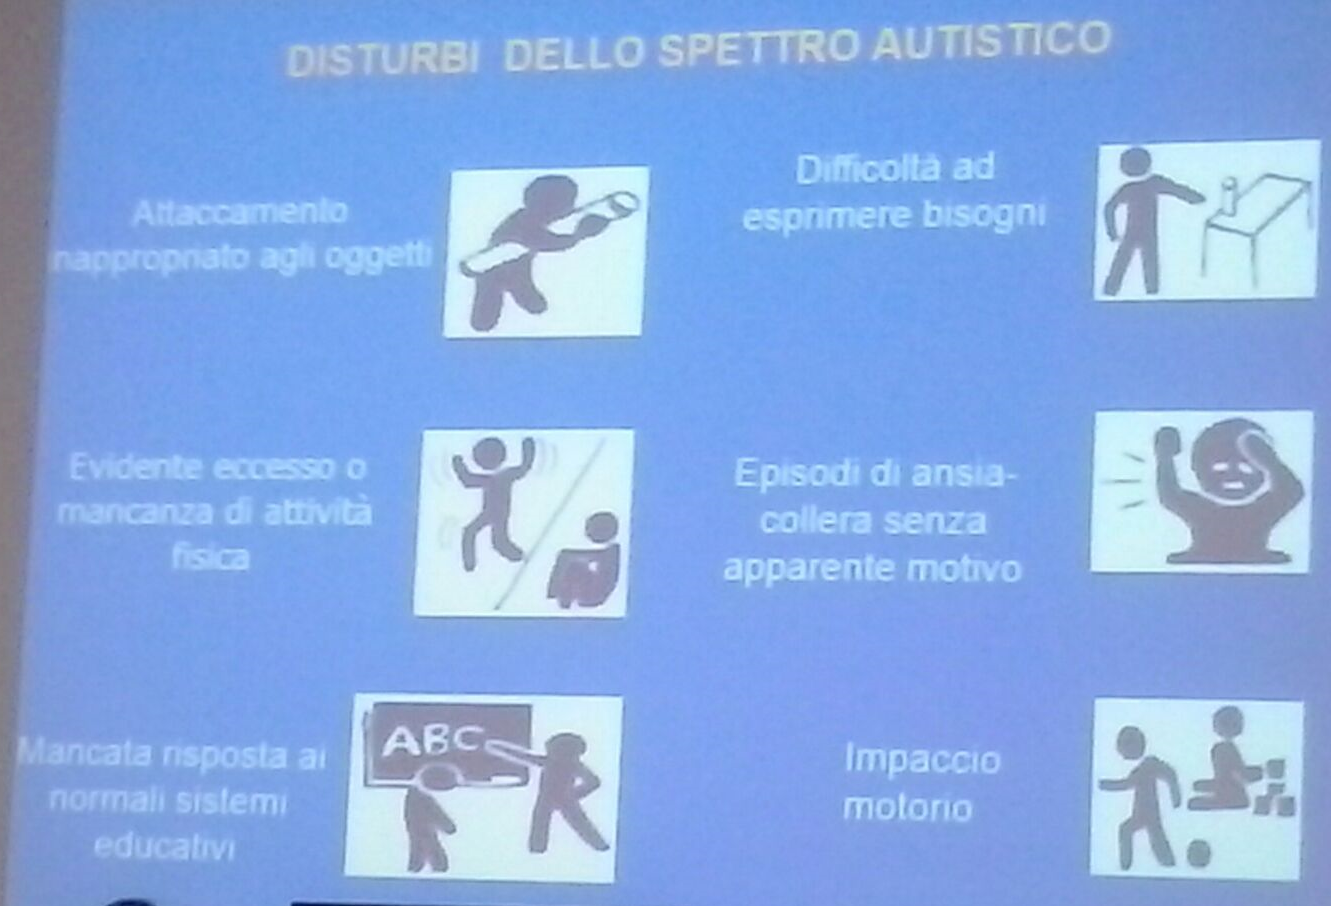
\includegraphics[width=6.67708in,height=4.55208in]{media/image2.png}

\begin{enumerate}
\def\labelenumi{\arabic{enumi}.}
\item
  \textbf{attaccamento inappropriato agli oggetti}: anche perché
  preferiscono di gran lunga gli oggetti alle persone. Ci sono poi degli
  oggetti a cui sono particolarmente legati, il cosiddetto ``oggetto
  autistico'' che può essere qualsiasi cosa, anche un pezzetto di legno.
  Tendono a preferire gli oggetti duri rispetto a quelli morbidi
\item
  \textbf{evidente eccesso o mancanza di attività fisica}: ipoattività o
  iperattività motoria
\item
  \textbf{mancata risposta ai normali sistemi educativi.} Non capiscono
  le richieste, e questo non è legato al livello di intelligenza ma alla
  percezione di quello che sentono e che vedono; probabilmente questo è
  dovuto a una mancata integrazione di questi stimoli a livello del SNC
\item
  \textbf{difficoltà ad esprimere bisogni}
\item
  \textbf{episodi di ansia/collera senza apparente motivo.} Noi non
  capiamo, può essere un cambiamento (esempio di una bambina che a
  scuola verso la fine del pranzo, in mensa, faceva crisi pazzesche, si
  disperava, si buttava per terra; per un anno educatori, insegnanti e
  genitori non hanno capito perché; poi si è scoperto che in quella
  scuola davano solitamente mele gialle, lei invece era abituata, a
  casa, a mangiare mele rosse)
\item
  \textbf{impaccio motorio.} Tipico soprattutto degli Asperger, mentre
  il bambino autistico grave è abilissimo dal punto di vista motorio
\end{enumerate}

\includegraphics[width=6.68750in,height=4.71875in]{media/image3.png}

\begin{enumerate}
\def\labelenumi{\arabic{enumi}.}
\item
  \textbf{apparente insensibilità al dolore, alle temperature}. Se
  cadono non piangono, se si scottano non piangono
\item
  \textbf{preferenza a rimanere solo, isolato}
\item
  \textbf{ruotare gli oggetti in modo ossessivo}. Particolare
  predilezione, probabilmente legato all'auto-sensorialità (è qualche
  cosa che parte da uno stimolo sensoriale e attraverso cui riusciamo a
  produrre/riprodurre delle sensazioni piacevoli ma in maniera
  indiretta: esempio il vezzo di arricciarsi una ciocca di capelli può
  essere legata alla concentrazione, al rilassamento o può anche essere
  banalmente piacevole, ha a che fare con l'auto-sensorialità. Il
  bambino autistico che ha bisogno di proteggersi dal mondo e dai suoi
  stimoli per lui incomprensibili, se ne difende procurandosi delle
  sensazioni -estremamente soggettive- che vedono la percezione
  oggettiva come uno strumento di mediazione: un passaggio che di per sé
  è solo un passaggio obbligato, ma quello che riesce a dare questa
  percezione viene vissuto in modo molto più intenso, e viene ricreata
  più e più volte, e la sensazione che se ne ricava aiuta a escludersi
  completamente dal mondo. Esempio: un bambino che passava intere ore
  con lo sguardo fuori dalla finestra e guardava il cielo con
  espressione di beatitudine: era la sensazione legata alla fonte
  luminosa o al colore, lui si perdeva, lo si chiamava ma non c'era
  verso di distoglierlo da questo guscio autosensoriale.
  L'autosensorialità è qualcosa che serve alla persona autistica a
  difendersi da tutti gli altri stimoli, da tutte le altre percezioni
  che non riesce a capire, che lo disorganizzano, lo destabilizzano,
  addirittura gli danno fastidio. Se mi avvolgo nelle sensazioni che
  provo come conseguenza a questo stimolo sensoriale, tutto mi riesce
  meno difficile, meno doloroso.
\item
  \textbf{Ecolalia}
\item
  \textbf{Mancata reciprocità}
\item
  \textbf{Mancata risposta alle indicazioni verbali}
\end{enumerate}

\emph{\textbf{{[}Breve focus sulla Sindrome di Asperger}}

Il tasso di prevalenza è di circa 5-6/1000.

Si differenzia dall'autismo perché

\begin{itemize}
\item
  non c'è un ritardo mentale
\item
  non c'è ritardo di linguaggio
\item
  c'è goffaggine motoria
\item
  diagnosi differenziale difficile coi disturbi di personalità
  (soprattutto schizoidi e disturbo ossessivo compulsivo)
\item
  orgoglio Aspie (termine da loro coniato): sono molto orgogliosi.
\end{itemize}

Autismo propriamente detto e Sindrome di Asperger sono la stessa entità?
Entità distinte? Non lo sappiamo. Certo prima del DSM 5 venivano tenuti
separati sotto la categoria DSA.{]}

La \textbf{triade di Wing} (studiosa di autismo, negli anni '80 ha dato
importanza agli studi di Asperger) vede le tre caratteristiche peculiari
di compromissioni dei DSA:

\begin{itemize}
\item
  socializzazione
\item
  comunicazione
\item
  interessi ristretti e ripetitivi
\end{itemize}

il DSM 5 ha aggiunto le anomalie sensoriali.

\emph{\textbf{Socializzazione}}: le anomalie della socializzazione
rappresentano il nucleo centrale. L'assenza di cognizione sociale
rappresenta non solo la caratteristica più peculiare, ma anche lo
``zoccolo duro'' dei DSA perché per quanto un bambino cresciuto possa
avere un'evoluzione positiva, quello della cognizione sociale rimane
l'aspetto su cui meno si può incidere; saranno sempre persone strane,
bizzarre. Esempio di un ragazzo, Asperger, laureato in architettura,
aveva 24 anni e non si era mai avvicinato a una ragazza. Ci avevamo
lavorato un po'. Poi un giorno, poco prima della laurea, alla fine della
lezione, aspetta la ragazza che gli piaceva e le dice ``scusi,
signorina, le interessano i miei appunti?'', capite che la ragazza non
lo degnò di uno sguardo e lui ci rimase malissimo, non capiva perché non
avesse accolto la sua proposta! Per lui i suoi appunti erano la cosa più
preziosa che aveva (in generale gli Asperger prendono la scuola, i voti,
molto sul serio).

Isolamento e chiusura sono tipici ma non assoluti, l'interazione e
l'iniziativa sociale possono essere presenti ma in modo inappropriato o
bizzarro (come questo ragazzo). Ci sono persone autistiche davvero
irraggiungibili; altre che si isolano ma se andate a stimolarle in
qualche modo rispondono. Il grado e la qualità di isolamento sono
diversi.

\emph{\textbf{Comunicazione}}:

Il linguaggio può essere

\begin{itemize}
\item
  assente,
\item
  oppure presente, anomalo o inadeguato -- sia per quanto riguarda la
  prosodia, che è sempre alterata, sia per il tono, l'aderenza al
  contesto (parliamo di pere e lui inizia a parlare di treni),
  l'ecolalia (caratteristica nei bambini, ripetono quello che sentono,
  se fate una domanda ripetono la domanda anziché rispondere), a volte
  coniano dei termini, tipica nei bambini è l'inversione pronominale
  (parlano di sé ma in seconda persona).
\end{itemize}

La comprensione è variabile, può essere

\begin{itemize}
\item
  assente,
\item
  apparentemente assente (esempio: un bambino che fino a 8 anni non
  stava in classe per più di 10-15 minuti, un giorno durante un incontro
  con altri bambini era particolarmente inquieto e, trovando una matita
  e un foglio di carta scrisse ``palla'' e noi capimmo che era in grado
  di scrivere anche se come avesse imparato per noi rimane un mistero.
  Nulla nel suo comportamento faceva pensare che trovasse il modo di
  recepire le cose in maniera tale da imparare a scrivere),
\item
  buona, ma con difficoltà nella comprensione di metafore, ironia,
  battute di spirito (non dite mai ``ho un diavolo per capello'', non
  capirebbe). Lo si può abituare, può imparare a riconoscere le
  metafore. Per capire che è un modo per dire un'altra cosa c'è bisogno
  di più passaggi, di più rappresentazioni, e le persone autistiche
  probabilmente non sono in grado di compiere questi passaggi.
\end{itemize}

Alcuni di loro non parlano e non comunicano, altri parlano ma non
comunicano (esempio: un bambino che parlava soltanto attraverso i
numeri. Aveva una prosodia anche molto efficace ``ventiquattro
venticinque sette quarantanove'' come dire ``posso uscire fuori dalla
stanza'', lui utilizzava i numeri. Un altro bambino invece utilizzava le
sillabe. Ci dicono cose per noi assurde, incomprensibili), altri ancora
comunicano ma con scarsa partecipazione emotiva. Certamente quello che
contraddistingue la comunicazione delle persone autistiche è la mancanza
di intenzionalità comunicativa, a loro interessa poco comunicare con gli
altri, perché gli altri sono poco interessanti.

\emph{\textbf{Anomalie sensoriali}}: presente una iperreattività o
iporeattività agli stimoli sensoriali, oppure un interesse insolito
verso aspetti sensoriali dell'ambiente. Per esempio c'è una risposta
spropositata ai \textbf{suoni} (di natura diversa, intensità diversa,
esempio un fischio, il tamburellare delle dita sul tavolo,
l'aspirapolvere), alle \textbf{consistenze} (è difficile che i bambini
autistici partecipino ai ``paciughi'' che fanno al nido o alla materna,
detestano sporcarsi le mani; la consistenza è anche relativa al cibo,
bambini che si nutrono solo di yogurt, altri solo di cose secche, o un
solo tipo di frutta, o ad un solo tipo di temperatura), agli
\textbf{odori} (più facile negli autistici gravi, portano tutto al naso,
esplorano col naso anziché con la bocca come fanno solitamente i
bambini) e \textbf{toccano tutto} (classico vederli camminare col
braccio proteso, sfiorano le pareti, tutto), mangiano la terra perché ne
adorano la consistenza.

La fascinazione visiva di \textbf{luci e movimenti}, luci per quello che
dicevo prima, i movimenti per via dell'autosensorialità (classico il
cestello della lavatrice in centrifuga, le cordine o i lacci che si
portano sempre appresso e fanno girare. Guardare costantemente un
oggetto che si muove alla stessa intensità, nello stesso modo,
ripetutamente da una sensazione che ci fa perdere psichicamente, da una
sensazione di chiusura ed estraneità nei confronti di tutto il resto).

\emph{\textbf{Attività e interess}}i: certamente questo comportamento
strano, bizzarro, ripetitivo che noi definiremmo disadattato (o
disadattivo) più di ogni altra cosa caratterizza il bambino autistico
rendendocelo incomprensibile. Probabilmente questo bisogno che tutto si
ripeta sempre allo stesso modo, il bisogno di compiere movimenti e cose
sempre allo stesso modo per un tempo indefinito, ha a che fare da una
parte con il bisogno di \textbf{immutabilità}, dall'altra li aiuta a
mantenere questa \textbf{chiusura difensiva} nei confronti di una realtà
difficilmente comprensibile da parte loro perché caotica, perché troppo
ricca di variabili -- noi non facciamo caso a quante cose, nel giro di
10 secondi, cambiano intorno a noi; una persona autistica che invece è
legata fortemente a questa immutabilità nota anche i più piccoli
cambiamenti.

Due estratti da persone Asperger:

\emph{``La realtà per una persona autistica è una massa interattiva e
confusa di eventi, persone, luoghi, segnali. Niente sembra avere limiti
netti, ordine o significato. Gran parte della mia vita è stata dedicata
al tentativo di scoprire il disegno nascosto di ogni cosa. La routine,
scadenze predeterminate, percorsi e rituali aiutano a introdurre un
ordine in una situazione inesorabilmente caotica'' }

\emph{Therese Jollife}

\emph{``Sono mal equipaggiato per sopravvivere in questo mondo, come un
extraterrestre che si sia perso senza un manuale per sapere come
orientarsi'' }

\emph{Sinclair}

La persona autistica sembra impossibilitata a filtrare, organizzare e
integrare ciò che percepisce. Quindi tutto diventa difficile da capire:
tutte le richieste dell'ambiente, tra cui anche quelle delle persone, i
causa-effetto, le parole, le regole sociali. Ha poi molta difficoltà a
regolare l'attenzione, non perché manchi, ma perché la loro attenzione
va tutta a dei particolari che noi non riusciamo neanche a vedere; la
difficoltà sta poi nel cogliere l'insieme di tutti questi particolari e
di riorganizzarli in modo da darci un senso. Questo passaggio, loro non
sono in grado di farlo.

\emph{``Quello che è normale per altre persone, non è normale per me.
Quello che io ritengo normale, non lo è per gli altri'' }

\emph{Sinclair}

\emph{\textbf{Autismo e intersoggettività}}

Il paziente autistico sembra non avere accesso all'intersoggettività,
funzione innata da cui dipende l'intero sviluppo mentale del bambino.
L'intersoggettività primaria è una sorta di ``percezione'' dell'altro,
uno spazio mentale che ha al centro due persone: nell'intersoggettività
primaria di un bambino di tre mesi questo spazio è costituito dalla
diade ``lui-la madre'', il mondo è tutto lì.

È presente sin dalla nascita, è appurato, e il bambino è in grado di
imitare sin dalla nascita e non solo percepire l'altro, ma anche le
intenzioni, le modalità di stare con l'altro. Tutto questo serve per
costruire il proprio mondo interpersonale e accedere anche al senso di
sé. Attraverso l'intersoggettività quindi il bambino capisce non solo il
comportamento della madre, ma anche e soprattutto la reciprocità di
questo, rispetto al proprio comportamento: accede così alla condivisione
dell'esperienza, al piacere di stare con l'altro, di fare qualcosa
insieme all'altro.

\emph{Qualcuno dice a Temple Grandin, famosissima Asperger: }

\emph{``non dovresti evitare il contatto con le persone'', }

\emph{e lei risponde: }

\emph{``ma lo sai che mi fanno male''.}

Rende bene l'idea degli altri che creano qualcosa di doloroso. Non si
può accedere al rapporto con l'altro, alla reciprocità,
all'intersoggettività: \textbf{gli altri fanno male}.

\emph{\textbf{Diagnosi}}

Gli elementi cardine sono:

\begin{itemize}
\item
  quadro clinico
\item
  test diagnostici (CARS, ADOS, ADI-R: i primi due fatti al bambino,
  l'ADI-R consta di domande ai genitori)
\item
  anamnesi: fondamentale perché se alcuni particolari segni sono
  comparsi nei primi 3 anni di vita, noi possiamo pensare alla diagnosi
  di DSA, diversamente no; è importante poi sapere che ci sono alcune
  tappe dello sviluppo che il bambino salta.
\end{itemize}

Per la diagnosi differenziale sono dirimenti le seguenti
caratteristiche:

\begin{itemize}
\item
  assenza di intenzionalità comunicativa
\item
  assenza di disponibilità di interazione
\item
  assenza di flessibilità cognitiva
\item
  l'età di comparsa
\end{itemize}

e va posta con:

\begin{itemize}
\item
  il ritardo mentale
\item
  DOC (disturbo ossessivo compulsivo)
\item
  Disturbo schizoide di personalità
\item
  Sindrome da deprivazione (studi in bambini messi in orfanatrofio,
  soprattutto in quelli dell'Est, presentavano un quadro clinico molto
  simile a quello dell'autismo; mutando ambiente, più accogliente e
  improntato ad affettività e reciprocità, nel giro di 2-3 anni
  cambiavano!)
\item
  Gravi deficit sensoriali (un bambino cieco, se non lo si diagnostica,
  può diventare autistico, o meglio ha una reazione autistica -- non si
  tratta di autismo primario. Vale anche per alcuni bambini sordi. Il
  bambino assume tratti autistici)
\item
  Mutismo elettivo (si manifesta solo in alcuni contesti, la persona
  autistica ha questi comportamenti sempre e con chiunque invece)
\item
  Schizofrenia a sintomatologia prevalentemente negativa
\end{itemize}

Conosciamo molte cose, gran parte però (soprattutto il perché e cosa
succeda) non lo sappiamo. Di certo possiamo dire che:

\begin{itemize}
\item
  compare entro i primi tre anni di vita
\item
  le cause sono sconosciute
\item
  la multifattorialità è l'ipotesi più ragionevole, più di un fattore
  incide sulla propensione all'autisticità
\item
  il rapporto maschi:femmine è di 4:1
\item
  ha una durata tendenzialmente lifelong
\item
  ormai per gli interventi più sono precoci e più sono efficaci (c'è un
  25-30\% che o esce dalla diagnosi di DSA o ne mantiene caratteristiche
  molto sfumate).
\end{itemize}

\emph{\textbf{Tipologie di soggetti autistici}}

Ci sono \textbf{autistici distaccati}, che tendono a usare l'altro come
una protesi (un classico è prendere la mano dell'adulto e metterla sulla
maniglia della porta perché l'adulto la apre), \textbf{autistici
passivi}, che però se stimolati rispondono, e ci sono \textbf{autistici
che hanno una certa iniziativa di interazione}, ma lo fanno in maniera
bizzarra e in linea di massima sempre improntata a una scarsa
reciprocità.

\emph{\textbf{Comorbidità}}

\textbf{Neurologica:}

\begin{itemize}
\item
  \textbf{ritardo mentale}, attenzione
\item
  \textbf{epilessia}, compare nel 25-30\% in età adolescenziale,
  talvolta anche prima
\item
  \textbf{anomalie genetiche} (sclerosi tuberosa, fenilchetonuria)
\item
  \textbf{anomalie cromosomiche} (X-fragile)
\end{itemize}

Il ritardo mentale può essere grave (50\% dei casi), medio-lieve (30\%)
o assente (20\%). L'associazione autismo-ritardo mentale è una questione
ancora aperta perché troppo facilmente l'autismo viene confuso con il
ritardo perché è sufficiente vedere una persona rispondere o non
rispondere alle sollecitazioni dell'ambiente per dire che ha ritardo
mentale. No!alla base potrebbe anche esserci un quadro autistico. E
nella diagnosi differenziale la capacità di socializzare, la
disponibilità di interazione, sono mantenute nel ritardo mentale.

\textbf{Psichiatrica:}

spesso presente, tanto che non è facile distinguere quello che è dovuto
all'autismo e quello che è dovuto a disturbi psicopatologici. Non è
facile perché il comportamento autistico può mascherare o prevalere sul
disturbo psichiatrico, dando un quadro difficile da trattare perché la
comorbidità psichiatrica non viene fuori semplicemente come in altri
casi.

\begin{itemize}
\item
  \textbf{disturbi dell'umore}, indipendentemente dal livello di
  funzionamento cognitivo, certo in adolescenza sembra abbiano una
  percezione dolorosa della propria diversità e quindi sono spesso
  soggetti a disturbi dell'umore, che però non manifestano! Non
  aspettatevi che un autistico smetta di mangiare, o abbia disturbi del
  sonno, non si manifesta quindi in maniera classica. Aumenta invece l'
  ``autisticità'', i comportamenti autistici peggiorano. La comorbidità
  psichiatrica risulta quindi mascherata dal comportamento autistico
\item
  \textbf{disturbi d'ansia}
\item
  \textbf{disturbi di personalità}, soprattutto negli Asperger
\end{itemize}

\emph{\textbf{Prognosi}}

\begin{itemize}
\item
  QI: si dice che quanto più è elevato il QI, tanto più è favorevole la
  prognosi.
\item
  Linguaggio comunicativo entro i 5 anni: anche qui prognosi più
  favorevole
\item
  Setback phenomenon: definito come un arresto di sviluppo nel bambino
  di 1-2 anni che fino ad allora ha avuto un accrescimento normale;
  prognosi più sfavorevole rispetto a insorgenze fin dalla nascita
\item
  Comorbidità
\end{itemize}

L'assenza di flessibilità cognitiva, l'assenza di iniziativa agli
scambi, l'assenza di capacità empatica, in sintesi l'assenza di
interesse per l'altro e per tutto ciò che lo circonda, rappresentano
fattori prognostici sfavorevoli.

\emph{\textbf{Eziopatogenesi }}

Moltissime le ipotesi eziopatogenetiche, nessuna esaustiva. I dati a
disposizione sono tanti e incoerenti tra di loro: nel 25-30\% dei casi
di uno studio X abbiamo risultati che poi non vengono riprodotti nello
studio successivo, o vengono addirittura negati. Certamente non abbiamo
prove di alterazione specifiche sia per quanto riguarda la
neurobiologia, sia per quanto riguarda i neurotrasmettitori, né prove di
alterazioni specifiche elettrofisiologiche, né genetiche, né
neuro-anatomiche. Dati che potrebbero essere importanti non vengono però
replicati, oppure hanno percentuali tali da non essere significativi da
un punto di vista statistico.

La \textbf{vulnerabilità genetica} è un fattore ritenuto dai più
indiscutibile. Ci sarebbe una sorta di predisposizione su cui vanno ad
agire molti altri fattori di natura ambientale che possono rendere
questa vulnerabilità qualcosa di clinicamente più importante e forte, o
possono invece smorzarla. Si è visto che nelle famiglie dove c'è un
bambino autistico, gli altri figli e i genitori possono presentare dei
tratti autistici, definiti ``\textbf{fenotipi estesi o allargati}'': ci
sono delle anomalie sottosoglia presenti anche in altri membri della
famiglia dunque.

\textbf{L'ambiente resta comunque determinante}. Tra i fattori
ambientali si annoverano: candidosi intestinale, vaccini, e tanti altri.
C'è maggiore rischio che questa vulnerabilità diventi più forte quando
la mamma del bambino è depressa: essa è presa dalla propria sofferenza
che non riesce a supplire alle esigenze di intersoggettività del
bambino.

Interessante è che forse, alla base dell'autismo, c'è una
\textbf{disabilità intersoggettiva}, sociale, con tutto quello che ne
consegue: la realtà, le persone, gli altri vengono registrati da un
punto di vista sensoriale e basta, senza che l'esperienza degli altri e
della realtà arrivi mai a formare dei contenuti mentali e a depositarli.

È stato ipotizzato che un'alterazione all'interno del circuito dei
\emph{mirrors} (neuroni specchio) renda la persona autistica incapace di
comprendere e condividere intuitivamente, immediatamente, ciò che
l'altro sta facendo e quindi le sue motivazioni ad agire. In questo modo
non abbiamo accesso alla dimensione intersoggettiva e quindi alla
comprensione dell'altro, del mondo, e del sé. Tutto diventa poco chiaro:
l'altro, il funzionamento dell'altro, del mondo, le sue richieste, e
quant'altro.

\emph{\textbf{Terapia}}

Non esistono interventi che curino la compromissione originaria -- anche
perché non la conosciamo.

Non c'è un intervento d'elezione.

Taluni affermano anche che l'andamento dell'autismo sia indipendente dal
trattamento.

Per l'esperienza è fondamentale l'integrazione tra interventi:

\begin{itemize}
\item
  \textbf{abilitativo} (la riabilitazione prevede un'azione che non c'è
  più; nell'autismo invece è da acquisire ex novo)
\item
  \textbf{psico-educativo} (l'educatore media con una
  persona/l'ambiente/le richieste dell'ambiente)
\item
  \textbf{psico-sociale} (l'adattamento alla realtà e l'autonomia
  sociale)
\item
  \textbf{farmacologico}
\end{itemize}

Su quest'ultimo possiamo contare poco perché nessun farmaco, ad oggi, si
è mostrato capace di curare l'autismo.

Interveniamo farmacologicamente quando i disturbi comportamentali sono
di entità tale da compromettere pesantemente la qualità di vita della
persona autistica, tale da rovinare la vita o da impedire l'inizio del
percorso abilitativo e psico-educativo.

Può essere utile un \textbf{neurolettico} da somministrare per breve
periodo e alla minore dose possibile: i neurolettici abbassano infatti
tutto lo psichismo, e se l'intervento più importante è l'abilitativo,
noi non possiamo smorzare lo psichismo. Tra i neurolettici quello che
funziona meglio è l'aloperidolo; altri farmaci sono psicotossici nel
soggetto autistico o inefficaci nel controllare la sintomatologia
comportamentale.

Interveniamo farmacologicamente soprattutto nei disturbi di comorbidità
visti prima, anche se qui la reattività è diversa rispetto ad altri
soggetti: nei DOC o nei disturbi dell'umore, se volessimo intervenire
con SSRI, non sortiremmo gli stessi benefici che nelle persone a
sviluppo normotipico.

Nei soggetti con DSA si hanno poi maggiormente effetti collaterali.

Negli adulti c'è un'efficacia maggiore.

Il rischio è che si abusi di interventi farmacologici in sostituzione di
quelli educativo e abilitativo.

\textbf{Il percorso abilitativo, se ben condotto, da miglioramenti
comportamentali veramente drastici:} nel momento in cui la persona
autistica riesce, attraverso un trattamento individualizzato, ad
esprimere bisogni ed emozioni con linguaggio verbale o con supporti
(immagini solitamente, loro prediligono il canale visivo: comunicazione
aumentativa alternativa), non è più soggetta a scoppi di rabbia (eventi
che rendono l'autismo così spaventoso e che ne determinano talvolta il
ricovero). Prevenire quindi i comportamenti problematici attraverso
l'adattamento ai contesti di vita.

In uno spazio dove deve vivere un ragazzo autistico tutto deve essere
indicato: immagini anche stilizzate dei luoghi e delle cose, di tutta la
realtà, questo basta per iniziare a orientarsi nello spazio.
Fondamentali le agende visive e la scomposizione dei vari atti, ad
esempio se vogliamo educare ad andare in bagno o fare un uovo al
tegamino: basta scomporre le immagini sequenza per sequenza. Si tratta
semplicemente di rendergli comprensibile la realtà, come devono essere
fatte le cose; se parlo non gli arriva nulla, o poco, o in modo caotico.

\end{document}

\section{Suicidio}

Dal punto di vista psichiatrico, il \textbf{\emph{suicidio}} può essere
considerato come la \emph{risposta dell'uomo alla mancanza di
significato del suo vivere}, essendo dettato da diversi moti emotivi
coscienti ed incoscienti, ed esprime una fuga dall'angoscia, ritenuta
intollerabile.
\\\\
Il suicidio è un'\emph{urgenza psichiatrica}, per cui da un punto di
vista medico l'obiettivo consiste nella riduzione o nella rimozione
delle cause e nel creare delle prospettive alternative di fuga, sia
questa reale o psicologica.
\\\\
Il suicidio costituisce quindi la \emph{conclusione di numerosi disturbi
psichiatrici}, ma quello in cui si osserva più comunemente è la
\textbf{depressione}, infatti il paziente depresso si suicida nel
tentativo di liberarsi da una condizione che sente altrimenti di non
poter modificare, cioè è convinto di non poter guarire e nella morte
pensa di trovare l'unica cosa che possa porre fine alla propria
sofferenza. Inoltre, in alcuni casi (soprattutto quando nella
depressione predominano dei forti sensi di colpa), il suicidio può
assumere una connotato di espiazione, come una sorta di
\emph{purificazione e riparazione per le proprie colpe}. Il
\textbf{\emph{tentativo di suicidio}} compare in genere nella \emph{fase
di remissione iniziale}, quando permane ancora una forte angoscia, ma il
paziente recupera un discreto grado di pianificazione ed ideazione, per
cui soprattutto in questa fase non si deve tralasciare il rischio di
suicidio, soprattutto se sono presenti degli elementi predisponenti come
i \emph{sentimenti di colpa}, l'\emph{ipocondria grave}, la
\emph{perdita di controllo} o i \emph{precedenti tentativi di suicidio}.
Altri elementi che possono giocare un ruolo nella predisposizione al
suicidio sono poi le \emph{incomprensioni da parte della famiglia}, la
\emph{presenza di una grave patologia organica} e le \emph{difficoltà
finanziarie e sociali rilevanti}.
\\\\
Negli \textbf{schizofrenici}, invece, il tentativo di suicidio è un
evento di difficile previsione, ed è del tutto \emph{incomprensibile},
attuandosi peraltro con \emph{modalità inconsuete}, manifestandosi
principalmente nella fase iniziale dell'acme dell'esperienza
catastrofica o nella fase di remissione, cioè quando il paziente diventa
in parte consapevole della propria condizione.
\\\\
In caso di tentativo di suicidio, inoltre, si devono stabilire le
\textbf{modalità} \textbf{adottate dal soggetto}, il \textbf{tipo di
eventuali strumenti lesivi usati}, la \textbf{gravità delle lesioni}, la
\textbf{minaccia di un'azione lesiva ritardata}, il \textbf{tipo di
paziente} ed i \textbf{precedenti psicopatologici}.
\\\\
Nella maggior parte dei casi si opta in genere per il \emph{ricovero
tempestivo}, anche se in altri casi si può optare per una \emph{terapia
a domicilio}, comunque con visite frequenti se il paziente è cooperante.
Pazienti molto a rischio sono poi gli \textbf{uomini} \textbf{anziani}
al di sopra dei 75 anni, in cui il suicidio fa spesso seguito ad un
evento di vita traumatico, che il paziente non riesce ad accettare o a
metabolizzare, anche se negli ultimi anni si è assistito ad un aumento
dell'incidenza del suicidio negli adolescenti.
\\\\
Esiste poi una classificazione del suicidio, proposta alla fine dell'800
da Emile Durkheim, in base alla quale si possono distinguere:

\begin{itemize}
\item
  \textbf{\emph{Suicidio Egoistico}}, cioè una condizione in cui
  l'individuo è scarsamente integrato nel contesto sociale, tende
  all'isolamento e quindi all'individuazione, e questo porta ad una
  condizione di egoismo affettivo.
\item
  \textbf{\emph{Suicidio Altruistico}}, che è l'opposto del suicidio
  egoistico, cioè in cui vi è una scarsa individualizzazione che porta
  poi all'identificazione nel gruppo.
\item
  \textbf{\emph{Suicidio Anomico}}, che si caratterizza per un
  cambiamento drastico, drammatico delle condizioni sociali, che può
  portare l'individuo a commettere suicidio, ad esempio a seguito di
  crolli economici e o dissesti finanziari importanti nell'ambito della
  società, e l'individuo si sente praticamente abbandonato dalla
  società.
\end{itemize}

È molto importante, inoltre, distinguere tra \textbf{tentativi di
suicidio completi}, in cui c'è l'intenzionalità a morire, e
\textbf{tentativi incompleti}, in cui si ricerca invece aiuto o
attenzione dagli altri; quest'ultimo tipo è caratteristico dei
\emph{disturbi di personalità di cluster B}, soprattutto il DP
borderline, mentre negli anziani sono più comuni i tentativi indiretti,
come il non assumere più i farmaci, o non seguire in maniera adeguata il
trattamento.

\section{Trattamento Sanitario Obbligatorio (TSO)}

L'articolo 32 della Costituzione Italiana afferma che ``\emph{La
Repubblica tutela la salute come diritto fondamentale dell'individuo ed
interesse della collettività, garantendo le cure anche agli
indigenti}''. Tuttavia, sempre nella Costituzione si afferma che
``\emph{Nessuno può essere obbligato ad un determinato trattamento
sanitario se non per disposizione di legge. La legge non può in nessun
caso violare i limiti imposti dal rispetto della persona umana}.''
\\\\
Il bene della vita, della salute e dell'integrità fisica e psichica sono
dunque oggetto dei diritti della persona, e si tratta di diritti
naturali essenziali ed assoluti, e come tali indisponibili,
irrinunciabili, non trasmissibili e non espropriabili. Da ciò deriva
quindi che gli accertamenti ed i trattamenti sanitari sono di norma
volontari, ovvero basati sul consenso, ed i provvedimenti obbligatori,
disposti secondo la legge, devono comunque rispettare la dignità della
persona, prestando sempre garanzie e diritti ai cittadini. Pertanto, per
poter procedere con un trattamento medico o anche con accertamenti
diagnostici rilevanti è necessario ottenere il \textbf{\emph{consenso}}
del paziente, il quale dev'essere:

\begin{itemize}
\item
  \textbf{Personale};
\item
  \textbf{Libero e Spontaneo};
\item
  \textbf{Consapevole ed Informato};
\item
  \textbf{Attuale};
\item
  \textbf{Gratuito};
\item
  \textbf{Manifesto}.
\end{itemize}

Il consenso non coincide con l'\textbf{assenso}, cioè col semplice
benestare, l'acconsentire passivo a qualcosa; il consenso richiede
infatti un incontro di volontà, di alleanze e di partecipazione attiva.
Il consenso informato è una decisione condivisa all'interno di una
relazione di cura fondata sulla fiducia e la chiarezza comunicativa.
\\\\
In ambito psichiatrico, tuttavia, i disturbi mentali possono determinare
assenza di consapevolezza di malattia e, sulla base di rappresentazioni
e valutazioni gravemente alterate, vengono rifiutati interventi sanitari
necessari ed urgenti, per cui in questi casi si può effettuare un
trattamento sanitario obbligatorio (TSO), il quale costituisce l'estremo
mezzo per rendere effettivo il diritto alla salute di un individuo con
una grave patologia psichica di cui non è consapevole.
\\\\
Il TSO, in ogni caso, è effettuato non come misura di ``difesa
sociale'', ma come recupero dell'individuo alla collettività, inoltre il
TSO deve sempre essere accompagnato dalla ricerca del consenso di chi vi
è obbligato.
\\\\
Per poter effettuare un TSO, devono essere quindi soddisfatte \emph{3
condizioni}:

\begin{itemize}
\item[1.]
  \textbf{Dev'essere presente un'alterazione psichica tale} (cioè
  talmente grave) \textbf{da richiedere interventi terapeutici urgenti,
  ovvero non differibili nel tempo};
\item[2.]
  \textbf{Gli interventi terapeutici non vengono accettati dall'infermo}
  (ed il rifiuto è strettamente legato al disturbo mentale);
\item[3.]
  \textbf{Non sussistono le condizioni e le circostanze per attuare
  idonei e tempestivi interventi in ambito extra-ospedaliero}.
\end{itemize}

\subsection{Procedura del TSO}

\begin{itemize}
\item
  Un medico (qualsiasi medico) visita la persona e, se ritiene che
  sussistano le tre condizioni di legge, prepara una proposta motivata
  di TSO in triplice copia con firma autografa.
\item
  Un secondo medico dell'Unità sanitaria locale visita la persona e
  redige il documento di convalida della proposta, sempre in triplice
  copia con firma autografa.
  
N.B.: In questa fase è necessario anche documentare tutti i tentativi
fatti per assicurare il consenso e la partecipazione da parte di chi vi
è obbligato, anche per far fronte a eventuali contestazioni e ricorsi
all'autorità amministrativa e al tribunale territoriale.

\item
  I documenti di proposta e convalida del TSO vengono recapitati,
  tramite la Polizia Municipale, al Sindaco, il quale emette l'ordinanza
  di TSO, che viene eseguita sempre dalla polizia municipale di concerto
  col personale sanitario fino al ricovero, che può avvenire solo presso
  l'SPDC.
\end{itemize}

Il TSO ha una durata massima di \emph{7 giorni}; se vengono meno le
condizioni, il TSO, può comunque essere revocato prima dal direttore del
SPDC, che lo comunica al sindaco, oppure, se persistono le condizioni,
il direttore del SPDC può chiedere al sindaco che ha emesso l'ordinanza
di TSO la proroga (eventualmente ripetuta più volte) motivate,
indicandone la durata presunta.

\subsection{Garanzie del TSO}

L'ordinanza del TSO va notificata alla persona che vi è sottoposta, la
quale conserva tutti i suoi diritti civili e politici, compreso quello
di comunicare, e deve essere sempre accompagnato dalla ricerca del
consenso e dal rispetto della dignità della persona. Il TSO, inoltre,
non viene annotato in nessun documento, né nel casellario o non comporta
la perdita della patente eccetera. Inoltre, entro 48 ore, il sindaco
deve inviare l'ordinanza al Giudice Tutelare, il quale, entro altre 48
ore, assunte le informazioni e gli eventuali accertamenti, provvede con
decreto motivato a convalidare o non convalidare il provvedimento del
sindaco. Il giudice tutelare può adottare provvedimenti urgenti per
amministrare il patrimonio della persona, e chi è sottoposto a TSO o
chiunque vi abbia interesse, può fare ricorso presso il tribunale
competente, che decide entro 30 giorni dal ricorso.

\subsection{Condizioni che non richiedono il TSO}

Esistono delle condizioni che, presentandosi urgenti e complesse, non
richiedono l'attivazione delle procedure del TSO, in quanto la persona è
incapace di esprimersi rispetto alla proposta di cura, e in questo caso
la priorità è la tutela della salute della persona, interessata da gravi
compromissioni dello stato di coscienza e dall'impossibilità di
esprimere o negare il consenso (ad esempio per traumi, intossicazioni,
delirium e demenze). In questi casi, infatti, si applica l'articolo 54
del codice penale, cioè lo stato di necessità.

\subsection{Limiti del TSO}

Il TSO \emph{non può essere effettuato per obbligare una persona ad
effettuare interventi diagnostici e terapeutici} per altre patologie
internistiche o chirurgiche, anche se indicate o prescritte dai medici o
con un alto rapporto benefici/rischi; in questi casi, molto complessi,
può essere necessario o opportuno coinvolgere il magistrato. Altri
limiti del TSO risiedono nel fatto che \emph{non esistono leggi che
obbligano la persona con disturbi mentali a seguire le cure a
domicilio}, e in questi casi è necessaria la ricerca del consenso, e
\emph{non rientra nelle competenze dei medici e degli psichiatri la
protezione dei familiari rispetto ai conviventi violenti}, e in questi
casi solo un giudice, in base agli articoli 342 bis e ter del codice
civile può disporre l'allontanamento della persona violenta.

\subsection{TSO Extra-Ospedaliero e TSO nei Minori}

Se sussistono le prime due condizioni per il TSO ma non la terza può
essere proposto un TSO extra-ospedaliero, che di solito viene usato solo
per l'effettuazione di terapie depot di pazienti in cura ai CSM.
\\\\
Nei minori, invece, va sempre ricercato il consenso sia del minore che
della famiglia, e in questi casi si possono riscontrare due condizioni:

\begin{itemize}
\item
  \emph{Minore bisognoso di cure urgenti e consenziente al trattamento,
  ma genitori contrari, e in questi casi è necessario ricorrere al TSO};
\item
  \emph{Minore bisognoso di cure urgenti, non consenziente, e genitori
  favorevoli, in questo caso non servirebbe il TSO formale, ma il
  rifiuto del minore dev'essere valutato e documentato}.
\end{itemize}

In entrambi i casi è utile informare il Tribunale per i Minori, in
particolare se l'ambiente familiare non è adeguato (\textbf{articolo 403
del codice civile}).

\subsection{Accertamento Sanitario Obbligatorio (ASO)}

L\textbf{'ASO} è un \emph{accertamento sanitario obbligatorio}
effettuato quando si ha il fondato sospetto sulla prima condizione di
legge prevista per poter intervenire in forma obbligatoria, e in cui
l'approfondimento diagnostico necessario non viene accettato dal
paziente. Si tratta comunque di un intervento eccezionale, che va sempre
preceduto ed accompagnato dalla ricerca del consenso. La proposta di ASO
può essere effettuata dal medico che ha constatato la presenza delle
condizioni sopracitate e previste dalla legge, e in questo caso, ai fini
dell'emissione dell'ordinanza di ASO da parte del sindaco basta la sola
certificazione medica di proposta, in triplice copia, contenente le
motivazioni dettagliate che sostengono la richiesta; a seguito
dell'ordinanza del sindaco la polizia municipale ed il personale
sanitario accompagnano la persona nel luogo stabilito per la visita, e
deve assicurare la sua presenza fino al termine della stessa.
\\\\
La legge, inoltre, prevede che l'ASO non possa avvenire in regime di
ricovero, ma può essere effettuato presso il PS, il CSM o in
ambulatorio, e l'esito può essere notevolmente diverso, ad esempio si
può avere una restituzione al medico di medicina generale, la presa in
cura al CSM, il ricovero volontario o anche un TSO, ma in ogni caso
l'esito dell'ASO va comunicato al Sindaco.





\end{document}
